\documentclass[11pt,a4paper,twoside]{book}
\usepackage[T1]{fontenc}
\usepackage[utf8]{inputenc}
\usepackage{mathpazo}
\usepackage[scaled=0.90]{helvet}
\usepackage{courier}
\usepackage[a4paper,inner=3.0cm,outer=2.4cm,top=2.6cm,bottom=2.8cm]{geometry}
\usepackage{xcolor}
\usepackage{tikz}
\usetikzlibrary{calc,positioning,arrows.meta,decorations.pathmorphing}
\usepackage{booktabs}
\usepackage{array}
\usepackage{longtable}
\usepackage{enumitem}
\usepackage[german=quotes]{csquotes}
\usepackage{fancyhdr}
\usepackage{titlesec}
\usepackage{amsmath,amssymb}
\usepackage{tcolorbox}
\tcbuselibrary{skins,breakable}
\usepackage[hidelinks]{hyperref}

\definecolor{tief}{HTML}{1F3A5F}
\definecolor{mittel}{HTML}{2E5F8A}
\definecolor{akzent}{HTML}{A34A28}
\definecolor{sand}{HTML}{F4F1EA}
\definecolor{grau}{HTML}{5A5A5A}
\definecolor{gruen}{HTML}{2F6B4F}
\definecolor{purpur}{HTML}{5B3A72}

\newcolumntype{P}[1]{>{\raggedright\arraybackslash}p{#1}}

\newcommand{\kursiv}[1]{{\itshape\color{grau}#1}}
\newcommand{\code}[1]{{\ttfamily\small #1}}
\newcommand{\Person}[1]{\textbf{#1}}
\newcommand{\Begriff}[1]{\textbf{#1}}
\newcommand{\zit}[1]{\textsuperscript{[#1]}}
\newcommand{\Oh}{\mathcal{O}}
\newcommand{\boxtitel}[1]{{\bfseries\color{tief}#1}\par\vspace{6pt}}
\newcommand{\boxtitelr}[1]{{\bfseries\color{akzent}#1}\par\vspace{6pt}}
\newcommand{\boxtitelg}[1]{{\bfseries\color{gruen}#1}\par\vspace{6pt}}
\newcommand{\boxtitelp}[1]{{\bfseries\color{purpur}#1}\par\vspace{6pt}}
\newcommand{\boxtitelm}[1]{{\bfseries\color{mittel}#1}\par\vspace{6pt}}
\newcommand{\loesung}{\par\vspace{8pt}{\bfseries\color{mittel}Lösung}\par\vspace{4pt}}
\newcommand{\schritt}[1]{\par\vspace{5pt}{\bfseries\color{grau}#1}\par\vspace{2pt}}

% Graphentheoretische Notation
\newcommand{\Gr}{G}
\newcommand{\Kn}[1]{K_{#1}}
\newcommand{\Kmn}[2]{K_{#1,#2}}
\newcommand{\Grad}{\deg}
\newcommand{\Nb}{N}
\newcommand{\chrom}{\chi}
\newcommand{\Ecken}{V}
\newcommand{\Kanten}{E}

\newtcolorbox{grundbox}[1][tief]{
  breakable, enhanced, colback=sand, colframe=sand,
  boxrule=0pt, leftrule=3pt, borderline west={3pt}{0pt}{#1},
  left=12pt, right=10pt, top=10pt, bottom=10pt,
  sharp corners, before skip=12pt, after skip=12pt}

\newenvironment{merksatz}{\begin{grundbox}[tief]}{\end{grundbox}}
\newenvironment{warnung}{\begin{grundbox}[akzent]}{\end{grundbox}}
\newenvironment{definition}{\begin{grundbox}[mittel]}{\end{grundbox}}
\newenvironment{geschichte}{\begin{grundbox}[gruen]}{\end{grundbox}}
\newenvironment{forschung}{\begin{grundbox}[purpur]}{\end{grundbox}}
\newenvironment{aufgabe}{\begin{grundbox}[grau]}{\end{grundbox}}

\titleformat{\chapter}[display]
  {\normalfont\huge\bfseries\color{tief}}{\Large\color{grau}Kapitel \thechapter}{8pt}{\Huge}
\titleformat{\part}[display]
  {\normalfont\huge\bfseries\color{tief}\filcenter}{\Large\color{grau}Teil \thepart}{10pt}{\Huge}
\titlespacing*{\chapter}{0pt}{10pt}{28pt}

\pagestyle{fancy}
\fancyhf{}
\fancyhead[LE,LO]{\small\itshape\color{grau}\leftmark}
\fancyfoot[LE,LO]{\small\color{grau}\thepage}
\renewcommand{\headrulewidth}{0.4pt}
\renewcommand{\footrulewidth}{0pt}
\renewcommand{\chaptermark}[1]{\markboth{#1}{}}
\setlength{\parindent}{0pt}
\setlength{\parskip}{6pt}
\renewcommand{\arraystretch}{1.3}

\renewcommand{\contentsname}{Inhaltsverzeichnis}
\renewcommand{\chaptername}{Kapitel}
\renewcommand{\partname}{Teil}
\renewcommand{\appendixname}{Anhang}
\renewcommand{\tablename}{Tabelle}
\renewcommand{\figurename}{Abbildung}

\hyphenation{Gra-phen-theo-rie Kno-ten-men-ge Kan-ten-men-ge Nach-bar-schaft
Zu-sam-men-hangs-kom-po-nen-te Zu-sam-men-hangs-kom-po-nen-ten Iso-mor-phie
Ad-ja-zenz-ma-trix In-zi-denz-ma-trix Span-nbaum Span-nbäume Dop-pel-zäh-lung
Hand-schlag-lem-ma Eu-ler-zug Eu-ler-zü-ge Ha-mil-ton-kreis Ha-mil-ton-krei-se
Pla-na-ri-tät Fär-bung Fär-bun-gen Vier-far-ben-satz Fünf-far-ben-satz
chro-ma-tisch chro-ma-ti-sche chro-ma-ti-schen Po-ly-nom Paa-rung Paa-run-gen
Fluss-netz-werk Schnitt-ka-pa-zi-tät ex-tre-mal ex-tre-ma-le Re-gu-la-ri-täts-lem-ma
Zu-falls-graph Zu-falls-gra-phen Ei-gen-wert Ei-gen-wer-te Ex-pan-der
Gra-phen-mi-nor Gra-phen-mi-no-ren Voll-stän-dig-keit Ge-gen-bei-spiel
Kno-ten-grad Kno-ten-gra-de Grad-fol-ge Teil-graph Teil-gra-phen
Kom-ple-ment-graph Mehr-fach-kan-te Mehr-fach-kan-ten}

\tikzset{
  knoten/.style={circle, fill=tief, inner sep=0pt, minimum size=5.5pt},
  knotenb/.style={circle, draw=tief, fill=white, line width=0.9pt, inner sep=1pt, minimum size=15pt, font=\scriptsize},
  knotenr/.style={circle, draw=akzent, fill=akzent!12, line width=0.9pt, inner sep=1pt, minimum size=15pt, font=\scriptsize},
  knoteng/.style={circle, draw=gruen, fill=gruen!12, line width=0.9pt, inner sep=1pt, minimum size=15pt, font=\scriptsize},
  kante/.style={draw=grau, line width=0.9pt},
  kanted/.style={draw=akzent, line width=1.5pt},
}

\begin{document}
\frontmatter
\begin{titlepage}
\centering
\vspace*{1.6cm}
{\footnotesize\scshape\color{grau} Mathematik von Grund auf --- Band 16}\\[1.9cm]
{\Huge\bfseries\color{tief} Punkte und Linien}\\[16pt]
{\Large\color{akzent} Graphentheorie}\\[1.5cm]

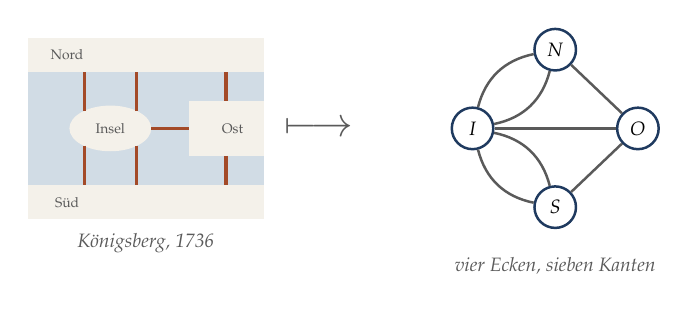
\begin{tikzpicture}[scale=1.0]
% Koenigsberg: schematisch
\begin{scope}[xshift=-3.3cm]
\fill[mittel!22] (-1.5,-1.15) rectangle (1.5,1.15);
\fill[sand] (-1.5,0.72) rectangle (1.5,1.15);
\fill[sand] (-1.5,-1.15) rectangle (1.5,-0.72);
\fill[sand] (0.55,-0.35) rectangle (1.5,0.35);
\fill[sand] (-0.45,0) ellipse (0.52 and 0.29);
\draw[akzent, line width=1.3pt] (-0.78,0.22) -- (-0.78,0.72);
\draw[akzent, line width=1.3pt] (-0.12,0.22) -- (-0.12,0.72);
\draw[akzent, line width=1.3pt] (-0.78,-0.22) -- (-0.78,-0.72);
\draw[akzent, line width=1.3pt] (-0.12,-0.22) -- (-0.12,-0.72);
\draw[akzent, line width=1.3pt] (0.07,0) -- (0.55,0);
\draw[akzent, line width=1.3pt] (1.02,0.35) -- (1.02,0.72);
\draw[akzent, line width=1.3pt] (1.02,-0.35) -- (1.02,-0.72);
\node[font=\tiny, color=grau] at (-1.0,0.94) {Nord};
\node[font=\tiny, color=grau] at (-1.0,-0.94) {Süd};
\node[font=\tiny, color=grau] at (-0.45,0) {Insel};
\node[font=\tiny, color=grau] at (1.1,0.0) {Ost};
\node[font=\scriptsize\itshape, color=grau] at (0,-1.45) {Königsberg, 1736};
\end{scope}

\node[font=\Large, color=grau] at (-1.1,0) {$\longmapsto$};

% Graph
\begin{scope}[xshift=1.9cm]
\node[knotenb] (N) at (0,1.0) {$N$};
\node[knotenb] (S) at (0,-1.0) {$S$};
\node[knotenb] (I) at (-1.05,0) {$I$};
\node[knotenb] (O) at (1.05,0) {$O$};
\draw[kante] (I) to[bend left=32] (N);
\draw[kante] (I) to[bend right=32] (N);
\draw[kante] (I) to[bend left=32] (S);
\draw[kante] (I) to[bend right=32] (S);
\draw[kante] (I) -- (O);
\draw[kante] (N) -- (O);
\draw[kante] (S) -- (O);
\node[font=\scriptsize\itshape, color=grau] at (0,-1.75) {vier Ecken, sieben Kanten};
\end{scope}
\end{tikzpicture}

\vspace{1.5cm}
{\large\color{grau} Von den Königsberger Brücken bis zum Regularitätslemma}\\[6pt]
{\color{grau} Jeder Schritt erklärt. Mit vollständig durchgerechneten Übungsaufgaben.}\\[2.0cm]
{\small\color{grau} Stand der Forschung: August 2026}
\end{titlepage}
\thispagestyle{empty}
\vspace*{\fill}
\begin{flushleft}
{\small\color{grau}
\textbf{\color{tief}Mathematik von Grund auf} --- Band 16\\[2pt]
\textit{Punkte und Linien} $\cdot$ Graphentheorie\\[14pt]

Herausgeber und Urheber: Jürgen Maier\\[2pt]
Entstanden 2026 in Zusammenarbeit mit Claude (Anthropic); Konzeption, Vorgaben, Prüfung und Herausgeberschaft: Jürgen Maier.\\[14pt]

\textbf{Lizenz}\\[2pt]
Dieses Werk ist lizenziert unter einer Creative-Commons-Lizenz \textbf{Namensnennung -- Weitergabe unter gleichen Bedingungen 4.0 International (CC BY-SA 4.0)}. Sie dürfen das Werk vervielfältigen, verbreiten, bearbeiten und auch kommerziell nutzen, sofern Sie den Urheber nennen und Bearbeitungen unter derselben Lizenz weitergeben.\\[2pt]
Lizenztext: \texttt{https://creativecommons.org/licenses/by-sa/4.0/legalcode.de}\\[14pt]

\textbf{Quellen und Fassungen}\\[2pt]
Quelltexte, Simulationen, Fehlermeldungen und aktuelle Fassungen aller Bände:\\
\texttt{https://github.com/juergenmaier2026/mathematik-von-grund-auf}\\[2pt]
Dauerhaft archiviert bei Zenodo: \texttt{https://doi.org/10.5281/zenodo.23698547}\\[14pt]

\textbf{Zitiervorschlag}\\[2pt]
Maier, J. (2026). \textit{Mathematik von Grund auf, Band 16: Punkte und Linien}. Fassung 1.0.1. \texttt{https://doi.org/10.5281/zenodo.23698547}\\[14pt]

Satz: \LaTeX{} mit Palatino. Fassung 1.0.1, Oktober 2026. 270 Seiten.
}
\end{flushleft}
\vspace*{1.5cm}

\tableofcontents
\mainmatter

\chapter*{Vorwort: Was dieser Band will}
\addcontentsline{toc}{chapter}{Vorwort}
\markboth{Vorwort}{Vorwort}

In Band 15 dieser Reihe, \kursiv{Die Kunst des Zählens}, steht die Graphentheorie als Teil~V: drei Kapitel, vierunddreißig Seiten. Das war zu wenig, und zwar nicht aus Platzgründen, sondern aus einem sachlichen: Die Graphentheorie ist kein Anhängsel der Kombinatorik. Sie ist ein eigenes Gebiet mit eigenen Fragen, eigenen Beweismethoden und einer eigenen Geschichte, die 1736 in Königsberg beginnt und heute in der Wahrscheinlichkeitstheorie, der Algebra und der theoretischen Informatik weitergeht.

Dieser Band holt das nach. Er setzt nichts voraus als die Bereitschaft, Definitionen ernst zu nehmen.

\begin{merksatz}
\boxtitel{Was Sie mitbringen müssen}
\begin{center}
\renewcommand{\arraystretch}{1.5}
\begin{tabular}{@{}P{3.2cm}P{5.8cm}@{}}
\toprule
\textbf{Mengen} & Was $\in$, $\subseteq$, $\cup$, $\cap$ bedeuten. Mehr nicht.\\
\textbf{Summenzeichen} & $\sum$ als abkürzende Schreibweise für \enquote{addiere alles auf}.\\
\textbf{Induktion} & Wird in Kapitel~4 noch einmal vollständig vorgeführt, bevor sie gebraucht wird.\\
\textbf{Matrizen} & Erst ab Kapitel~3, und dort wird erklärt, was eine Matrix ist.\\
\bottomrule
\end{tabular}
\end{center}

\begin{center}
\begin{minipage}{0.88\textwidth}
\kursiv{Wer Band 0 (\enquote{Die Kunst des Rechnens}) durchgearbeitet hat, hat alles. Wer das nicht hat, kommt trotzdem durch --- die vier Dinge oben werden im Text nachgereicht, wo sie zum ersten Mal auftreten.}
\end{minipage}
\end{center}
\end{merksatz}

\section*{Warum die Graphentheorie ein guter Einstieg ist}

Es gibt einen Grund, warum Vorlesungen über Graphentheorie oft im ersten Semester liegen, und er ist nicht, dass der Stoff leicht wäre. Er ist dieser: Die Gegenstände sind endlich, anschaulich und trotzdem tief.

Ein Graph ist nichts als eine endliche Menge von Punkten und eine Auswahl von Paaren dieser Punkte. Man kann ihn auf ein Blatt Papier zeichnen. Man kann ihn abzählen. Es gibt keine Grenzwerte, keine unendlichen Prozesse, keine Konvergenzfragen. Und dennoch enthält dieses schlichte Gebilde Probleme, an denen die besten Mathematiker Jahrzehnte gescheitert sind --- der Vierfarbensatz brauchte hundertvierundzwanzig Jahre, und die Hadwigersche Vermutung von 1943 ist bis heute offen.

\begin{merksatz}
\boxtitel{Was das für Sie bedeutet}
\begin{center}
\begin{minipage}{0.9\textwidth}
Sie können in diesem Gebiet \kursiv{jeden einzelnen Beweis vollständig nachvollziehen}, ohne irgendwo auf Vertrauen angewiesen zu sein. Und Sie stehen nach fünfzehn Kapiteln vor offenen Fragen, die Sie verstehen --- nicht vor offenen Fragen, von denen Sie gehört haben.
\end{minipage}
\end{center}
\end{merksatz}

\section*{Drei Warnungen}

\begin{warnung}
\boxtitelr{Erstens: Das Bild ist nicht der Graph}
Graphen werden gezeichnet, und die Zeichnung hilft. Sie führt aber auch in die Irre, weil derselbe Graph auf unendlich viele Weisen gezeichnet werden kann --- als übersichtliches Fünfeck oder als Knäuel, in dem sich Linien kreuzen.

\begin{center}
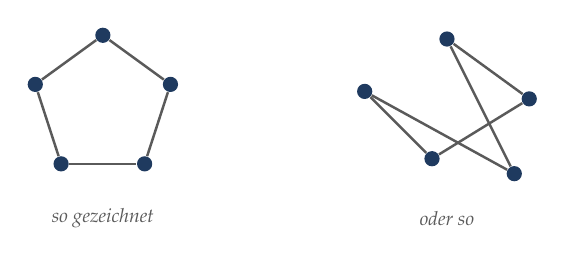
\begin{tikzpicture}[scale=0.95]
\begin{scope}
\foreach \i in {0,...,4} {
  \node[knoten] (a\i) at (90+72*\i:0.95) {};
}
\foreach \i/\j in {0/1,1/2,2/3,3/4,4/0} \draw[kante] (a\i) -- (a\j);
\node[font=\scriptsize\itshape, color=grau] at (0,-1.5) {so gezeichnet};
\end{scope}
\begin{scope}[xshift=4.6cm]
\node[knoten] (b0) at (0,0.9) {};
\node[knoten] (b1) at (1.1,0.1) {};
\node[knoten] (b2) at (-0.2,-0.7) {};
\node[knoten] (b3) at (0.9,-0.9) {};
\node[knoten] (b4) at (-1.1,0.2) {};
\draw[kante] (b0) -- (b1);
\draw[kante] (b1) -- (b2);
\draw[kante] (b2) -- (b4);
\draw[kante] (b4) -- (b3);
\draw[kante] (b3) -- (b0);
\node[font=\scriptsize\itshape, color=grau] at (0,-1.5) {oder so};
\end{scope}
\end{tikzpicture}
\end{center}

Beides ist derselbe Graph: fünf Ecken, jede mit genau zwei Nachbarn, alles in einem Kreis. Rechts kreuzen sich zwei Linien --- das ist eine Eigenschaft der \kursiv{Zeichnung}, nicht des Graphen. Kapitel~8 macht aus diesem Unterschied ein ganzes Thema.
\end{warnung}

\begin{warnung}
\boxtitelr{Zweitens: \enquote{Offensichtlich} ist hier besonders gefährlich}
Weil Graphen anschaulich sind, verleiten sie dazu, ein Bild für einen Beweis zu halten. Das geht sehr oft gut und gelegentlich furchtbar schief.

Ein Beispiel, das Sie in Kapitel~7 wiederfinden: \kursiv{Jeder zusammenhängende Graph, in dem jede Ecke mindestens zwei Nachbarn hat, enthält einen Kreis} --- das ist wahr und wird bewiesen. Und: \kursiv{Jeder zusammenhängende Graph, in dem jede Ecke mindestens zwei Nachbarn hat, enthält einen Kreis durch alle Ecken} --- das ist falsch, sieht aber genauso plausibel aus.

\begin{center}
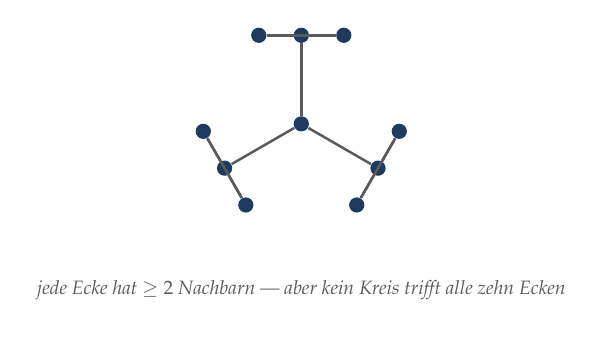
\begin{tikzpicture}[scale=0.9]
\node[knoten] (z) at (0,0) {};
\foreach \a in {90,210,330} {
  \node[knoten] (p\a) at (\a:1.25) {};
  \node[knoten] (q\a) at ($(\a:1.25)+(\a+90:0.6)$) {};
  \node[knoten] (r\a) at ($(\a:1.25)+(\a-90:0.6)$) {};
  \draw[kante] (z) -- (p\a);
  \draw[kante] (p\a) -- (q\a);
  \draw[kante] (p\a) -- (r\a);
  \draw[kante] (q\a) -- (r\a);
}
\node[font=\scriptsize\itshape, color=grau] at (0,-2.35) {jede Ecke hat $\ge 2$ Nachbarn --- aber kein Kreis trifft alle zehn Ecken};
\end{tikzpicture}
\end{center}
\end{warnung}

\begin{warnung}
\boxtitelr{Drittens: Die Bezeichnungen sind uneinheitlich}
Die Graphentheorie ist aus mehreren Quellen zusammengeflossen, und das hört man ihrer Sprache an. Dieselbe Sache heißt je nach Buch anders.

\begin{center}
{\small
\renewcommand{\arraystretch}{1.42}
\begin{tabular}{@{}P{2.6cm}P{3.0cm}P{2.6cm}@{}}
\toprule
\textbf{Hier} & \textbf{Auch üblich} & \textbf{Englisch}\\
\midrule
Ecke & Knoten, Punkt & vertex, node\\
Kante & Verbindung, Linie & edge, line\\
Grad & Valenz, Ordnung & degree, valency\\
Kreis & Zyklus & cycle\\
Weg & Pfad, Kantenzug & path\\
Paarung & Matching & matching\\
\bottomrule
\end{tabular}}
\end{center}

\begin{center}
\begin{minipage}{0.88\textwidth}
\kursiv{Dieser Band sagt durchgehend \enquote{Ecke} und \enquote{Kante}. Wenn Sie in einem anderen Buch \enquote{Knoten} lesen, ist dasselbe gemeint. Besonders heikel ist \enquote{Weg}: Manche Bücher erlauben dabei Wiederholungen von Ecken, andere nicht. Kapitel~2 legt das hier ein für alle Mal fest.}
\end{minipage}
\end{center}
\end{warnung}

\section*{Ein Beispiel gleich zu Beginn}

Damit Sie sehen, wohin die Reise geht, hier eine vollständige mathematische Argumentation --- lesbar, bevor Sie irgendetwas gelernt haben.

\begin{merksatz}
\boxtitel{Auf jeder Feier gibt es zwei Personen mit gleich vielen Bekannten}
\textbf{Die Behauptung.} Auf einer Feier mit $n \ge 2$ Personen gibt es stets zwei Personen, die gleich viele der Anwesenden kennen. (\enquote{Kennen} sei gegenseitig: Wenn $A$ die Person $B$ kennt, dann kennt $B$ auch $A$.)

\schritt{Schritt 1 --- Was kann eine einzelne Person überhaupt an Bekanntenzahlen haben?}
Eine Person kennt mindestens $0$ und höchstens $n-1$ der übrigen Anwesenden (sich selbst zählen wir nicht mit). Es gibt also $n$ mögliche Werte:
\[ 0,\ 1,\ 2,\ \ldots,\ n-1 . \]

\schritt{Schritt 2 --- Der scheinbare Widerspruch}
Wir haben $n$ Personen und $n$ mögliche Werte. Es könnte also sein, dass jede Person einen anderen Wert hat --- die Werte würden dann genau aufgebraucht.

\schritt{Schritt 3 --- Warum das nicht sein kann}
Nehmen wir an, alle $n$ Personen hätten verschiedene Bekanntenzahlen. Dann kommt jeder der $n$ Werte $0, 1, \ldots, n-1$ genau einmal vor. Insbesondere gibt es:
\begin{itemize}[leftmargin=1.4em, itemsep=2pt]
\item eine Person $X$ mit dem Wert $0$ --- sie kennt \kursiv{niemanden} der Anwesenden;
\item eine Person $Y$ mit dem Wert $n-1$ --- sie kennt \kursiv{alle} übrigen $n-1$ Anwesenden.
\end{itemize}

\schritt{Schritt 4 --- Der Widerspruch}
$Y$ kennt alle übrigen Anwesenden. Da $X$ nicht dieselbe Person wie $Y$ ist (sie haben ja verschiedene Werte, und $0 \neq n-1$ wegen $n \ge 2$), gehört $X$ zu diesen übrigen. Also kennt $Y$ die Person $X$.

Weil \enquote{Kennen} gegenseitig ist, kennt dann auch $X$ die Person $Y$. Damit kennt $X$ mindestens eine Person --- im Widerspruch zu $X$'s Wert $0$.

\schritt{Schritt 5 --- Schluss}
Die Annahme aus Schritt~3 führt auf einen Widerspruch. Also war sie falsch: Es können \kursiv{nicht} alle Bekanntenzahlen verschieden sein. Somit gibt es zwei Personen mit gleich vielen Bekannten. $\blacksquare$
\end{merksatz}

\begin{merksatz}
\boxtitel{Was an diesem Beweis bemerkenswert ist}
\begin{center}
\renewcommand{\arraystretch}{1.5}
\begin{tabular}{@{}P{3.0cm}P{6.0cm}@{}}
\toprule
\textbf{Kein Rechnen} & Es kommt keine einzige Rechnung vor --- nur genaues Hinsehen.\\
\textbf{Kein Beispiel} & Der Beweis gilt für \kursiv{jede} Feier, für $n=2$ ebenso wie für $n = 10^{9}$.\\
\textbf{Die Voraussetzung zählt} & Bei $n \ge 2$ ist $0 \neq n-1$. Bei $n=1$ wäre $0 = n-1$, und die Aussage wird sinnlos.\\
\textbf{Es war Graphentheorie} & Personen sind Ecken, Bekanntschaften sind Kanten, Bekanntenzahlen sind Grade.\\
\bottomrule
\end{tabular}
\end{center}

\begin{center}
\begin{minipage}{0.88\textwidth}
\kursiv{Die letzte Zeile ist der Punkt. Sie haben soeben Ihren ersten graphentheoretischen Satz bewiesen, ohne ein einziges Fachwort zu benutzen. In Kapitel~1 lernen Sie die Wörter --- der Gedanke bleibt derselbe.}
\end{minipage}
\end{center}
\end{merksatz}

\section*{Wie dieser Band aufgebaut ist}

\begin{merksatz}
\boxtitel{Sieben Teile, fünfzehn Kapitel}
\begin{center}
{\small
\renewcommand{\arraystretch}{1.42}
\begin{tabular}{@{}P{1.0cm}P{3.4cm}P{4.4cm}@{}}
\toprule
\textbf{Teil} & \textbf{Thema} & \textbf{Die Leitfrage}\\
\midrule
I & Der Begriff (1--3) & Was ist ein Graph, und wie schreibt man ihn auf?\\
II & Bäume (4--5) & Was ist die einfachste zusammenhängende Struktur?\\
III & Durchlaufen (6--7) & Kann man alles genau einmal besuchen?\\
IV & Zeichnen und Färben (8--10) & Wann geht es ohne Kreuzungen, mit wie vielen Farben?\\
V & Paarungen und Flüsse (11--12) & Wie viel passt gleichzeitig hindurch?\\
VI & Grenzen und Zufall (13--14) & Wie viele Kanten erzwingen eine Struktur?\\
VII & Aktueller Stand (15) & Was ist heute offen?\\
\bottomrule
\end{tabular}}
\end{center}
\end{merksatz}

Jedes Kapitel folgt demselben Rhythmus, den Sie aus den anderen Bänden kennen: Motivation, Definition, Begründung, Warnkasten, durchgerechnete Aufgabe mit Probe. Die Kästen sind farbig unterschieden --- blau für Merksätze, rot für Warnungen, grün für Geschichte und Herkunft, violett für den aktuellen Forschungsstand, blaugrau für Definitionen.

Und noch ein Wort zur Herkunft der Beispiele. Wo es sich anbietet, stammen sie aus der Klinik: Dienst\-pläne, Kon\-takt\-nach\-ver\-fol\-gung, Or\-gan\-zu\-tei\-lung, Bet\-ten\-be\-le\-gung. Das ist kein Zierrat. Die Graphentheorie ist in der Medizin an mehr Stellen im Einsatz, als man vermutet, und ein Beispiel, das man kennt, trägt einen Beweis weiter als eines, das man sich erst vorstellen muss.

\vspace{10pt}
\begin{flushright}
\itshape\color{grau}
Nichts ist selbstverständlich.\\
Nichts ist trivial.\\
Jeder Schritt wird erklärt.
\end{flushright}

\part{Der Begriff}

\chapter{Was ein Graph ist}

\section{Drei Fragen, die dieselbe Frage sind}

Beginnen wir mit drei Aufgaben, die nichts miteinander zu tun zu haben scheinen.

\begin{merksatz}
\boxtitel{Erste Frage --- die Brücken von Königsberg}
Die Stadt Königsberg lag im 18. Jahrhundert an beiden Ufern des Flusses Pregel. In der Mitte lag eine Insel, den Kneiphof, und weiter östlich, wo die beiden Flussarme sich vereinigen, ein weiteres Landstück. Sieben Brücken verbanden diese vier Landstücke.

\begin{center}
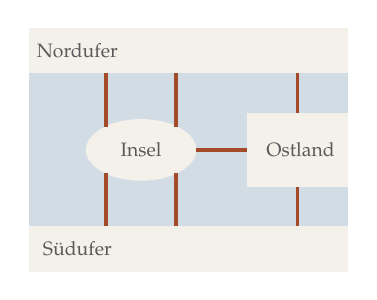
\begin{tikzpicture}[scale=1.35]
\fill[mittel!22] (-1.5,-1.15) rectangle (1.5,1.15);
\fill[sand] (-1.5,0.72) rectangle (1.5,1.15);
\fill[sand] (-1.5,-1.15) rectangle (1.5,-0.72);
\fill[sand] (0.55,-0.35) rectangle (1.5,0.35);
\fill[sand] (-0.45,0) ellipse (0.52 and 0.29);
\draw[akzent, line width=1.3pt] (-0.78,0.22) -- (-0.78,0.72);
\draw[akzent, line width=1.3pt] (-0.12,0.22) -- (-0.12,0.72);
\draw[akzent, line width=1.3pt] (-0.78,-0.22) -- (-0.78,-0.72);
\draw[akzent, line width=1.3pt] (-0.12,-0.22) -- (-0.12,-0.72);
\draw[akzent, line width=1.3pt] (0.07,0) -- (0.55,0);
\draw[akzent, line width=1.3pt] (1.02,0.35) -- (1.02,0.72);
\draw[akzent, line width=1.3pt] (1.02,-0.35) -- (1.02,-0.72);
\node[font=\scriptsize, color=grau] at (-1.05,0.93) {Nordufer};
\node[font=\scriptsize, color=grau] at (-1.05,-0.93) {Südufer};
\node[font=\scriptsize, color=grau] at (-0.45,0) {Insel};
\node[font=\scriptsize, color=grau] at (1.05,0.0) {Ostland};
\end{tikzpicture}
\end{center}

\textbf{Die Frage der Bürger:} Kann man einen Spaziergang machen, bei dem man jede der sieben Brücken \kursiv{genau einmal} überquert?
\end{merksatz}

\begin{merksatz}
\boxtitel{Zweite Frage --- der Dienstplan}
An einer Klinik sollen fünf Ärztinnen --- nennen wir sie $A$, $B$, $C$, $D$, $E$ --- auf Dienste verteilt werden. Manche Paare dürfen nicht dieselbe Schicht bekommen, weil sie sich sonst in der Facharztweiterbildung gegenseitig blockieren:

\begin{center}
{\small
\renewcommand{\arraystretch}{1.42}
\begin{tabular}{@{}P{3.0cm}P{4.4cm}@{}}
\toprule
\textbf{Unverträgliche Paare} & $AB$, $AC$, $BC$,\newline $BD$, $CE$, $DE$\\
\bottomrule
\end{tabular}}
\end{center}

\textbf{Die Frage der Oberärztin:} Wie viele verschiedene Schichten braucht man mindestens?
\end{merksatz}

\begin{merksatz}
\boxtitel{Dritte Frage --- die Kontaktnachverfolgung}
Auf einer Station wird bei einem Patienten ein multiresistenter Keim nachgewiesen. Das Hygieneteam hat notiert, wer in den letzten Tagen mit wem längeren Kontakt hatte.

\textbf{Die Frage des Hygieneteams:} Welche Personen können überhaupt betroffen sein --- und lässt sich die Station so in Gruppen zerlegen, dass zwischen den Gruppen kein einziger Kontakt bestand?
\end{merksatz}

Drei Fragen aus drei Welten. Was sie gemeinsam haben, sieht man erst, wenn man alles wegstreicht, was nicht zur Sache gehört.

\begin{merksatz}
\boxtitel{Was übrig bleibt, wenn man alles Überflüssige streicht}
\begin{center}
{\small
\renewcommand{\arraystretch}{1.5}
\begin{tabular}{@{}P{2.4cm}P{3.0cm}P{3.0cm}@{}}
\toprule
& \textbf{Die Dinge} & \textbf{Die Beziehung}\\
\midrule
Königsberg & Landstücke & \enquote{durch eine Brücke verbunden}\\
Dienstplan & Ärztinnen & \enquote{unverträglich}\\
Hygiene & Personen & \enquote{hatten Kontakt}\\
\bottomrule
\end{tabular}}
\end{center}

\begin{center}
\begin{minipage}{0.88\textwidth}
\kursiv{In allen drei Fällen gibt es eine endliche Menge von Dingen und eine Beziehung, die immer zwischen \kursiv{zwei} Dingen besteht und \kursiv{gegenseitig} ist: Wenn die Insel mit dem Nordufer durch eine Brücke verbunden ist, dann auch das Nordufer mit der Insel.}
\end{minipage}
\end{center}
\end{merksatz}

Genau dieses gemeinsame Skelett ist ein \Begriff{Graph}. Die Mathematik gewinnt ihre Kraft daraus, dass sie das Skelett einmal untersucht und die Ergebnisse dann allen drei Fragen zugleich zugutekommen.

\section{Die Definition --- Zeichen für Zeichen}

Jetzt kommt die Definition. Sie ist kurz, und sie enthält vier Zeichen, die vielleicht nicht selbstverständlich sind. Deshalb steht sie hier zuerst, und danach wird sie Stück für Stück auseinandergenommen.

\begin{definition}
\boxtitelm{Definition 1.1 --- Graph}
Ein \Begriff{Graph} ist ein Paar $G = (V, E)$, wobei
\begin{itemize}[leftmargin=1.4em, itemsep=3pt]
\item $V$ eine endliche, nichtleere Menge ist --- ihre Elemente heißen \Begriff{Ecken};
\item $E$ eine Menge von zweielementigen Teilmengen von $V$ ist --- ihre Elemente heißen \Begriff{Kanten}.
\end{itemize}
In Zeichen:
\[ E \subseteq \bigl\{\, \{u,v\} \;:\; u \in V,\; v \in V,\; u \neq v \,\bigr\}. \]
\end{definition}

Das war die Definition. Nun das Auseinandernehmen.

\begin{merksatz}
\boxtitel{Was jedes Zeichen bedeutet}
\begin{center}
{\small
\renewcommand{\arraystretch}{1.55}
\begin{tabular}{@{}P{1.6cm}P{7.0cm}@{}}
\toprule
$G$ & Der Name des Graphen. Ein Buchstabe, mehr nicht --- so wie eine Funktion \enquote{$f$} heißt.\\
$(V,E)$ & Ein \Begriff{geordnetes Paar}: zwei Dinge in fester Reihenfolge. Erst die Ecken, dann die Kanten. Das Komma trennt sie.\\
$V$ & Von lateinisch \kursiv{vertex}, Scheitelpunkt. Eine Menge, etwa $V = \{A, B, C, D, E\}$.\\
$E$ & Von englisch \kursiv{edge}, Kante. Ebenfalls eine Menge --- aber ihre \kursiv{Elemente} sind selbst wieder Mengen.\\
$\{u,v\}$ & Die Menge, die genau die beiden Ecken $u$ und $v$ enthält. Geschweifte Klammern bedeuten: \enquote{die Menge mit diesen Elementen}.\\
$\subseteq$ & \enquote{ist Teilmenge von}. $E \subseteq M$ heißt: Jedes Element von $E$ ist auch Element von $M$.\\
$u \neq v$ & \enquote{$u$ ist nicht dasselbe wie $v$}. Eine Kante verbindet zwei \kursiv{verschiedene} Ecken.\\
\bottomrule
\end{tabular}}
\end{center}
\end{merksatz}

Der Punkt, der am meisten Verwirrung stiftet, ist dieser: \textbf{Eine Kante ist eine Menge, keine Reihenfolge.} Das hat eine Folge, die wir sofort festhalten.

\begin{merksatz}
\boxtitel{Warum $\{u,v\}$ und $\{v,u\}$ dieselbe Kante sind}
Bei Mengen kommt es nicht auf die Reihenfolge an. Die Menge \enquote{die Zahlen 3 und 7} ist dieselbe, ob man sie als $\{3,7\}$ oder als $\{7,3\}$ aufschreibt. Beide haben genau dieselben Elemente, und mehr sagt eine Menge nicht aus.

Daher gilt
\[ \{u,v\} = \{v,u\}, \]
und deshalb bildet die Definition genau die \kursiv{gegenseitigen} Beziehungen ab, die wir im vorigen Abschnitt gefunden haben. Wäre eine Kante ein geordnetes Paar $(u,v)$, so wären $(u,v)$ und $(v,u)$ verschieden --- und wir hätten Einbahnstraßen statt Brücken.

\begin{center}
\begin{minipage}{0.86\textwidth}
\kursiv{Das ist kein Zufall und keine Schlamperei, sondern eine bewusste Entscheidung: Die Definition wurde so gebaut, dass sie die Beziehung abbildet, die wir untersuchen wollen. Für Einbahnstraßen gibt es einen anderen Begriff, den gerichteten Graphen --- Abschnitt 1.4.}
\end{minipage}
\end{center}
\end{merksatz}

\subsection*{Ein erstes vollständig ausgeschriebenes Beispiel}

\begin{merksatz}
\boxtitel{Der Dienstplan als Graph}
Wir schreiben die zweite Frage aus Abschnitt 1.1 vollständig als Graph auf.

\schritt{Die Eckenmenge}
\[ V = \{A,\, B,\, C,\, D,\, E\} \]
Fünf Ärztinnen, fünf Ecken.

\schritt{Die Kantenmenge}
Die unverträglichen Paare waren $AB$, $AC$, $BC$, $BD$, $CE$ und $DE$. Als Mengen geschrieben:
\[ E = \bigl\{\, \{A,B\},\ \{A,C\},\ \{B,C\},\ \{B,D\},\ \{C,E\},\ \{D,E\} \,\bigr\} \]

\schritt{Kontrolle}
$E$ hat sechs Elemente. Jedes davon ist eine zweielementige Teilmenge von $V$. Keine Kante verbindet eine Ecke mit sich selbst. Die Definition ist erfüllt.

\schritt{Und als Bild}
\begin{center}
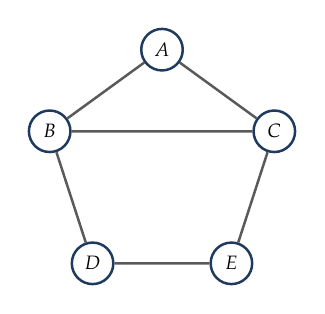
\begin{tikzpicture}[scale=1.25]
\node[knotenb] (A) at (90:1.2) {$A$};
\node[knotenb] (B) at (162:1.2) {$B$};
\node[knotenb] (C) at (18:1.2) {$C$};
\node[knotenb] (D) at (234:1.2) {$D$};
\node[knotenb] (E) at (306:1.2) {$E$};
\draw[kante] (A) -- (B);
\draw[kante] (A) -- (C);
\draw[kante] (B) -- (C);
\draw[kante] (B) -- (D);
\draw[kante] (C) -- (E);
\draw[kante] (D) -- (E);
\end{tikzpicture}
\end{center}

\begin{center}
\begin{minipage}{0.86\textwidth}
\kursiv{Das Bild und die beiden Mengen enthalten genau dieselbe Auskunft. Das Bild ist bequemer zu lesen, die Mengen sind eindeutig. Wo beide sich zu widersprechen scheinen, haben die Mengen recht.}
\end{minipage}
\end{center}
\end{merksatz}

\begin{merksatz}
\boxtitel{Zwei Zahlen, die man einem Graphen sofort ansieht}
\begin{center}
\renewcommand{\arraystretch}{1.5}
\begin{tabular}{@{}P{2.6cm}P{2.0cm}P{3.6cm}@{}}
\toprule
\textbf{Name} & \textbf{Zeichen} & \textbf{Bedeutung}\\
\midrule
Ordnung & $|V|$ oder $n$ & Anzahl der Ecken\\
Größe & $|E|$ oder $m$ & Anzahl der Kanten\\
\bottomrule
\end{tabular}
\end{center}

Die senkrechten Striche $|\cdot|$ bedeuten \enquote{Anzahl der Elemente}. Im Dienstplanbeispiel ist $n = |V| = 5$ und $m = |E| = 6$.

\begin{center}
\begin{minipage}{0.86\textwidth}
\kursiv{Die Wörter sind unglücklich gewählt --- \enquote{Größe} meint die Kantenzahl, nicht die Eckenzahl --- aber sie sind seit hundert Jahren eingebürgert. Merken Sie sich lieber $n$ und $m$; diese beiden Buchstaben werden in der gesamten Literatur so verwendet.}
\end{minipage}
\end{center}
\end{merksatz}

\section{Warum gerade diese Definition?}

Eine Definition ist keine Entdeckung, sondern eine Entscheidung. Man hätte es auch anders machen können, und es lohnt sich zu sehen, was dabei jeweils herauskäme.

\begin{merksatz}
\boxtitel{Drei Dinge, die Definition 1.1 ausschließt}
\begin{center}
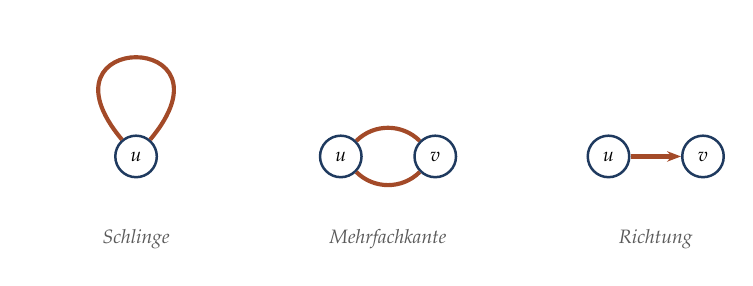
\begin{tikzpicture}[scale=1.0]
\begin{scope}
\node[knotenb] (x) at (0,0) {$u$};
\draw[kanted] (x) to[out=50,in=130,looseness=13] (x);
\node[font=\scriptsize\itshape, color=grau] at (0,-1.05) {Schlinge};
\end{scope}
\begin{scope}[xshift=3.2cm]
\node[knotenb] (p) at (-0.6,0) {$u$};
\node[knotenb] (q) at (0.6,0) {$v$};
\draw[kanted] (p) to[bend left=45] (q);
\draw[kanted] (p) to[bend right=45] (q);
\node[font=\scriptsize\itshape, color=grau] at (0,-1.05) {Mehrfachkante};
\end{scope}
\begin{scope}[xshift=6.6cm]
\node[knotenb] (r) at (-0.6,0) {$u$};
\node[knotenb] (s) at (0.6,0) {$v$};
\draw[kanted, -{Stealth[length=5pt]}] (r) -- (s);
\node[font=\scriptsize\itshape, color=grau] at (0,-1.05) {Richtung};
\end{scope}
\end{tikzpicture}
\end{center}

\begin{center}
{\small
\renewcommand{\arraystretch}{1.5}
\begin{tabular}{@{}P{2.6cm}P{2.6cm}P{3.4cm}@{}}
\toprule
\textbf{Verboten durch} & \textbf{Was fehlt} & \textbf{Wie es sonst heißt}\\
\midrule
$u \neq v$ & Schlingen & Graph \kursiv{mit} Schlingen\\
$E$ ist eine \kursiv{Menge} & Mehrfachkanten & \Begriff{Multigraph}\\
$\{u,v\}$ statt $(u,v)$ & Richtungen & \Begriff{gerichteter Graph}\\
\bottomrule
\end{tabular}}
\end{center}

\begin{center}
\begin{minipage}{0.88\textwidth}
\kursiv{Ein Graph nach Definition 1.1 heißt zur Betonung auch \Begriff{schlichter Graph} oder \Begriff{einfacher Graph}. Wenn in diesem Band ohne Zusatz \enquote{Graph} steht, ist immer Definition 1.1 gemeint.}
\end{minipage}
\end{center}
\end{merksatz}

Warum diese Verbote? Weil sie fast nichts kosten und viel einbringen.

\begin{merksatz}
\boxtitel{Was die Einschränkung einbringt}
\begin{center}
\renewcommand{\arraystretch}{1.5}
\begin{tabular}{@{}P{2.8cm}P{5.8cm}@{}}
\toprule
\textbf{Eindeutigkeit} & Zwischen zwei Ecken gibt es eine Kante oder keine. Man kann also von \enquote{der Kante zwischen $u$ und $v$} sprechen.\\
\textbf{Endliche Schranke} & Es gibt höchstens $\binom{n}{2}$ Kanten. Bei Mehrfachkanten wäre die Kantenzahl unbeschränkt.\\
\textbf{Einfache Sätze} & Fast alle Sätze dieses Bandes wären mit Mehrfachkanten umständlicher zu formulieren, ohne inhaltlich mehr zu sagen.\\
\bottomrule
\end{tabular}
\end{center}
\end{merksatz}

\begin{warnung}
\boxtitelr{Königsberg braucht aber Mehrfachkanten!}
Zwischen der Insel und dem Nordufer gibt es \kursiv{zwei} Brücken, zwischen Insel und Südufer ebenfalls. Der Königsberger Graph ist also kein Graph nach Definition 1.1, sondern ein Multigraph.

Das ist kein Versehen, sondern der Normalfall: Die Grundlagen werden für den einfachsten Begriff entwickelt, und wo ein Satz mehr verträgt, wird das ausdrücklich gesagt. Kapitel~6 --- die Eulerzüge --- ist genau so ein Ort: Der Satz von Euler gilt für Multigraphen, und dort wird der Begriff sauber erweitert.

\begin{center}
\begin{minipage}{0.88\textwidth}
\kursiv{Merken Sie sich das Muster. Es kommt in der Mathematik ständig vor: Man definiert eng, entwickelt die Theorie, und erweitert dort, wo man die Erweiterung wirklich braucht --- nicht vorsorglich.}
\end{minipage}
\end{center}
\end{warnung}

\subsection*{Die größtmögliche Kantenzahl}

\begin{merksatz}
\boxtitel{Wie viele Kanten kann ein Graph mit $n$ Ecken höchstens haben?}
\schritt{Die Frage}
$E$ besteht aus zweielementigen Teilmengen von $V$. Die größtmögliche Kantenmenge ist die, die \kursiv{alle} solchen Teilmengen enthält. Wie viele gibt es?

\schritt{Erste Zählung --- mit Doppelzählung}
Wir zählen zunächst \kursiv{geordnete} Paare $(u,v)$ mit $u \neq v$: Für $u$ gibt es $n$ Möglichkeiten, für $v$ dann noch $n-1$ (alle außer $u$). Das sind
\[ n \cdot (n-1) \quad \text{geordnete Paare.} \]

\schritt{Die Korrektur}
Jede Kante $\{u,v\}$ wurde dabei \kursiv{zweimal} gezählt: einmal als $(u,v)$ und einmal als $(v,u)$. Also teilen wir durch $2$:
\[ \frac{n(n-1)}{2} . \]

\schritt{Die übliche Schreibweise}
Diese Zahl schreibt man als \Begriff{Binomialkoeffizient}
\[ \binom{n}{2} = \frac{n(n-1)}{2}, \]
gelesen \enquote{$n$ über $2$}. Sie ist aus Band 15, Kapitel~2 bekannt und bedeutet dort dasselbe: die Anzahl der Möglichkeiten, aus $n$ Dingen zwei auszuwählen, ohne auf die Reihenfolge zu achten.

\schritt{Probe an kleinen Zahlen}
\begin{center}
\renewcommand{\arraystretch}{1.42}
\begin{tabular}{@{}P{1.2cm}P{2.6cm}P{3.4cm}@{}}
\toprule
$n$ & $\binom{n}{2} = \frac{n(n-1)}{2}$ & \textbf{Nachzählen}\\
\midrule
$2$ & $\frac{2 \cdot 1}{2} = 1$ & $\{A,B\}$ \quad --- stimmt\\
$3$ & $\frac{3 \cdot 2}{2} = 3$ & $AB, AC, BC$ --- stimmt\\
$4$ & $\frac{4 \cdot 3}{2} = 6$ & $AB, AC, AD$,\newline $BC, BD, CD$\\
$5$ & $\frac{5 \cdot 4}{2} = 10$ & \\
\bottomrule
\end{tabular}
\end{center}
\end{merksatz}

\section{Nachbarschaft und Grad}

\begin{definition}
\boxtitelm{Definition 1.2 --- benachbart, Nachbarschaft, Grad}
Sei $G = (V,E)$ ein Graph und $v \in V$ eine Ecke.
\begin{itemize}[leftmargin=1.4em, itemsep=4pt]
\item Zwei Ecken $u$ und $v$ heißen \Begriff{benachbart} (oder \Begriff{adjazent}), wenn $\{u,v\} \in E$ gilt.
\item Die \Begriff{Nachbarschaft} von $v$ ist die Menge aller Nachbarn:
\[ N(v) = \{\, u \in V \;:\; \{u,v\} \in E \,\}. \]
\item Der \Begriff{Grad} von $v$ ist die Anzahl seiner Nachbarn:
\[ \deg(v) = |N(v)| . \]
\end{itemize}
Eine Ecke mit $\deg(v) = 0$ heißt \Begriff{isoliert}.
\end{definition}

\begin{merksatz}
\boxtitel{Am Dienstplanbeispiel nachgerechnet}
Der Graph war
\[ E = \bigl\{ \{A,B\}, \{A,C\}, \{B,C\}, \{B,D\}, \{C,E\}, \{D,E\} \bigr\}. \]

\schritt{Nachbarschaften --- durch systematisches Durchgehen}
Für $A$: Wir gehen alle sechs Kanten durch und notieren die, in denen $A$ vorkommt. Das sind $\{A,B\}$ und $\{A,C\}$. Der jeweils \kursiv{andere} Eintrag ist der Nachbar:
\[ N(A) = \{B, C\}, \qquad \deg(A) = 2 . \]

Ebenso für die übrigen:
\begin{center}
\renewcommand{\arraystretch}{1.45}
\begin{tabular}{@{}P{1.2cm}P{3.2cm}P{2.2cm}P{1.6cm}@{}}
\toprule
\textbf{Ecke} & \textbf{Kanten mit ihr} & $N(v)$ & $\deg(v)$\\
\midrule
$A$ & $AB$, $AC$ & $\{B,C\}$ & $2$\\
$B$ & $AB$, $BC$, $BD$ & $\{A,C,D\}$ & $3$\\
$C$ & $AC$, $BC$, $CE$ & $\{A,B,E\}$ & $3$\\
$D$ & $BD$, $DE$ & $\{B,E\}$ & $2$\\
$E$ & $CE$, $DE$ & $\{C,D\}$ & $2$\\
\bottomrule
\end{tabular}
\end{center}

\schritt{Eine erste Beobachtung}
Die Summe aller Grade ist
\[ 2 + 3 + 3 + 2 + 2 = 12 = 2 \cdot 6 = 2m . \]
Das ist kein Zufall, wie der nächste Abschnitt zeigt.
\end{merksatz}

\begin{warnung}
\boxtitelr{Der Grad zählt Nachbarn, nicht Kanten --- meistens dasselbe}
In einem Graphen nach Definition 1.1 ist die Anzahl der Nachbarn gleich der Anzahl der Kanten, die an $v$ hängen --- denn jede solche Kante liefert genau einen Nachbarn, und verschiedene Kanten liefern verschiedene Nachbarn.

In einem \kursiv{Multigraphen} stimmt das nicht mehr: Bei zwei Brücken zwischen Insel und Nordufer hat die Insel einen Nachbarn, aber zwei Kanten. Dort definiert man den Grad über die \kursiv{Kanten}, weil das für die Sätze die richtige Zahl ist. Eine Schlinge zählt dabei $2$, weil sie an der Ecke zweimal ansetzt.

\begin{center}
\begin{minipage}{0.88\textwidth}
\kursiv{Für Königsberg heißt das: Die Insel hat Grad $5$ (zwei Brücken nach Norden, zwei nach Süden, eine nach Osten), die drei anderen Landstücke haben je Grad $3$. Behalten Sie diese vier Zahlen $5,3,3,3$ im Kopf --- in Kapitel~6 entscheiden sie die Frage der Bürger.}
\end{minipage}
\end{center}
\end{warnung}

\section{Das Handschlaglemma}

Der erste richtige Satz dieses Bandes. Er ist einfach, und er wird bis zum letzten Kapitel gebraucht.

\begin{merksatz}
\boxtitel{Satz 1.3 (Handschlaglemma)}
Für jeden Graphen $G = (V,E)$ gilt
\[ \sum_{v \in V} \deg(v) \;=\; 2 \cdot |E| . \]
In Worten: \kursiv{Die Summe aller Eckengrade ist doppelt so groß wie die Anzahl der Kanten.}
\end{merksatz}

\subsection*{Der Beweis --- und was daran das eigentliche Argument ist}

\begin{merksatz}
\boxtitel{Beweis durch Doppelzählung}
\schritt{Schritt 1 --- Wir erfinden etwas zum Zählen}
Betrachten wir alle Paare der Form
\[ (v, e) \quad \text{mit} \quad v \in V,\ e \in E,\ \text{und } v \text{ liegt auf } e . \]
Ein solches Paar heißt \Begriff{Inzidenz}: eine Ecke zusammen mit einer Kante, die sie berührt. Nennen wir die Anzahl aller Inzidenzen $Z$.

\begin{center}
\begin{minipage}{0.88\textwidth}
\kursiv{Warum tut man das? Weil man dieselbe Menge auf zwei Arten abzählen kann und dabei zwei verschiedene Ausdrücke bekommt --- die dann gleich sein müssen. Das ist die \Begriff{Doppelzählung}, die wichtigste Beweismethode der endlichen Mathematik.}
\end{minipage}
\end{center}

\schritt{Schritt 2 --- Erste Zählung: nach Ecken sortiert}
Wir gehen die Ecken der Reihe nach durch und fragen bei jeder: An wie vielen Inzidenzen ist sie beteiligt?

Eine Ecke $v$ liegt auf genau denjenigen Kanten, die $v$ als Element enthalten. Davon gibt es genau $\deg(v)$ Stück --- das ist die Definition des Grades. Also liefert die Ecke $v$ genau $\deg(v)$ Inzidenzen.

Jede Inzidenz hat genau eine Ecke, wird also bei genau einer Ecke gezählt. Aufsummieren über alle Ecken zählt daher jede Inzidenz genau einmal:
\[ Z = \sum_{v \in V} \deg(v) . \]

\schritt{Schritt 3 --- Zweite Zählung: nach Kanten sortiert}
Jetzt gehen wir die Kanten durch und fragen bei jeder: An wie vielen Inzidenzen ist sie beteiligt?

Eine Kante ist eine zweielementige Menge $e = \{u,v\}$. Auf ihr liegen genau die beiden Ecken $u$ und $v$ --- \kursiv{genau zwei}, weil $|e| = 2$ nach Definition und weil $u \neq v$ gilt. Also liefert jede Kante genau $2$ Inzidenzen.

Jede Inzidenz hat genau eine Kante, wird also bei genau einer Kante gezählt. Aufsummieren über alle Kanten:
\[ Z = \sum_{e \in E} 2 = 2 \cdot |E| . \]

\schritt{Schritt 4 --- Gleichsetzen}
In Schritt 2 und Schritt 3 haben wir dieselbe Zahl $Z$ ermittelt. Also:
\[ \sum_{v \in V} \deg(v) \;=\; Z \;=\; 2 \cdot |E| . \qquad \blacksquare \]
\end{merksatz}

\begin{merksatz}
\boxtitel{Dasselbe als Bild}
Man kann sich die Inzidenzen als \kursiv{Kantenenden} vorstellen. Jede Kante hat zwei Enden. Jedes Ende steckt in genau einer Ecke.

\begin{center}
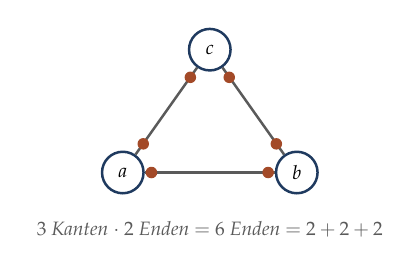
\begin{tikzpicture}[scale=1.3]
\node[knotenb] (a) at (0,0) {$a$};
\node[knotenb] (b) at (1.7,0) {$b$};
\node[knotenb] (c) at (0.85,1.2) {$c$};
\draw[kante] (a) -- (b);
\draw[kante] (a) -- (c);
\draw[kante] (b) -- (c);
\fill[akzent] (0.28,0) circle (1.6pt);
\fill[akzent] (1.42,0) circle (1.6pt);
\fill[akzent] (0.20,0.28) circle (1.6pt);
\fill[akzent] (0.66,0.93) circle (1.6pt);
\fill[akzent] (1.50,0.28) circle (1.6pt);
\fill[akzent] (1.04,0.93) circle (1.6pt);
\node[font=\scriptsize\itshape, color=grau] at (0.85,-0.55) {$3$ Kanten $\cdot$ $2$ Enden $=$ $6$ Enden $=$ $2+2+2$};
\end{tikzpicture}
\end{center}

Zählt man die Enden \kursiv{kantenweise}, bekommt man $2m$. Zählt man sie \kursiv{eckenweise}, bekommt man die Gradsumme. Es sind dieselben Enden.
\end{merksatz}

\begin{merksatz}
\boxtitel{Satz 1.4 --- Die Anzahl der Ecken ungeraden Grades ist gerade}
\textbf{Behauptung.} In jedem Graphen ist die Anzahl der Ecken mit ungeradem Grad eine gerade Zahl.

\schritt{Beweis --- Schritt 1: Die Ecken aufteilen}
Wir teilen $V$ in zwei Gruppen:
\[ V_{\text{g}} = \{\, v \in V : \deg(v) \text{ gerade} \,\}, \qquad
   V_{\text{u}} = \{\, v \in V : \deg(v) \text{ ungerade} \,\} . \]
Jede Ecke gehört zu genau einer der beiden Gruppen, denn jede ganze Zahl ist entweder gerade oder ungerade.

\schritt{Schritt 2 --- Die Gradsumme aufspalten}
\[ \sum_{v \in V} \deg(v) \;=\; \underbrace{\sum_{v \in V_{\text{g}}} \deg(v)}_{=: S_{\text{g}}} \;+\; \underbrace{\sum_{v \in V_{\text{u}}} \deg(v)}_{=: S_{\text{u}}} \]

\schritt{Schritt 3 --- Was wir über die drei Summen wissen}
\begin{center}
\renewcommand{\arraystretch}{1.5}
\begin{tabular}{@{}P{1.6cm}P{6.8cm}@{}}
\toprule
Gesamt & Nach Satz 1.3 ist $\sum_{v} \deg(v) = 2m$, also \textbf{gerade}.\\
$S_{\text{g}}$ & Eine Summe aus lauter geraden Zahlen ist \textbf{gerade}.\\
$S_{\text{u}}$ & Aus $S_{\text{u}} = 2m - S_{\text{g}}$ folgt: gerade minus gerade ist gerade, also ist $S_{\text{u}}$ \textbf{gerade}.\\
\bottomrule
\end{tabular}
\end{center}

\schritt{Schritt 4 --- Der Schluss auf die Anzahl}
$S_{\text{u}}$ ist eine Summe aus lauter \kursiv{ungeraden} Zahlen, und diese Summe ist gerade. Wie viele Summanden hat sie?

Addiert man ungerade Zahlen, so ist die Summe von $k$ ungeraden Zahlen genau dann gerade, wenn $k$ gerade ist. Denn jede ungerade Zahl lässt sich als $2a_i + 1$ schreiben, und
\[ \sum_{i=1}^{k} (2a_i + 1) = 2\Bigl(\sum_{i=1}^{k} a_i\Bigr) + k . \]
Der erste Summand ist gerade. Die Gesamtsumme ist also genau dann gerade, wenn $k$ gerade ist.

Da $S_{\text{u}}$ gerade ist, muss $k = |V_{\text{u}}|$ gerade sein. $\blacksquare$
\end{merksatz}

\begin{merksatz}
\boxtitel{Wofür man das braucht}
\begin{center}
\begin{minipage}{0.9\textwidth}
Satz 1.4 ist ein \kursiv{Unmöglichkeitswerkzeug}. Er beantwortet Fragen der Art \enquote{Kann es einen Graphen geben, bei dem \ldots?} mit einem klaren Nein.

\textbf{Beispiel.} Kann es in einer Gruppe von $15$ Personen sein, dass jede genau $3$ andere kennt? --- Nein. Es gäbe $15$ Ecken vom ungeraden Grad $3$, und $15$ ist ungerade. Nach Satz 1.4 unmöglich.

\textbf{Gegenprobe mit Satz 1.3.} $\sum \deg(v) = 15 \cdot 3 = 45 = 2m$ hieße $m = 22{,}5$ --- keine ganze Zahl. Beide Sätze zeigen dasselbe.
\end{minipage}
\end{center}
\end{merksatz}

\begin{geschichte}
\boxtitelg{Woher der Name \enquote{Handschlaglemma} kommt}
Deutet man die Ecken als Personen und die Kanten als Handschläge, so besagt Satz 1.3: \kursiv{Die Gesamtzahl der geschüttelten Hände ist doppelt so groß wie die Zahl der Handschläge} --- weil an jedem Handschlag zwei Hände beteiligt sind.

Das Wort \Begriff{Lemma} (griechisch \kursiv{lêmma}, \enquote{das Angenommene}) bezeichnet in der Mathematik einen Hilfssatz: ein Ergebnis, das man weniger um seiner selbst willen beweist als deshalb, weil man es später ständig braucht. Diese Einordnung ist eine Frage der Gewohnheit, nicht des Inhalts --- manches \enquote{Lemma} ist berühmter als die Sätze, für die es erfunden wurde. Das Handschlaglemma ist so ein Fall.
\end{geschichte}

\section{Welche Gradfolgen sind möglich?}

\begin{definition}
\boxtitelm{Definition 1.5 --- Gradfolge}
Die \Begriff{Gradfolge} eines Graphen ist die Liste der Grade aller Ecken, üblicherweise absteigend sortiert.
\end{definition}

Der Dienstplangraph hat die Gradfolge $(3,3,2,2,2)$.

Die naheliegende Umkehrfrage ist schwerer, als sie aussieht: Gegeben eine Zahlenfolge --- gibt es dazu einen Graphen?

\begin{merksatz}
\boxtitel{Zwei notwendige Bedingungen, die man sofort prüfen kann}
\begin{center}
\renewcommand{\arraystretch}{1.5}
\begin{tabular}{@{}P{1.2cm}P{7.2cm}@{}}
\toprule
(B1) & Die Summe aller Zahlen muss gerade sein (Satz 1.3).\\
(B2) & Jede Zahl muss zwischen $0$ und $n-1$ liegen, wobei $n$ die Anzahl der Zahlen ist --- mehr Nachbarn als andere Ecken kann keine Ecke haben.\\
\bottomrule
\end{tabular}
\end{center}

\begin{center}
\begin{minipage}{0.88\textwidth}
\kursiv{\textbf{Achtung:} Diese Bedingungen sind \kursiv{notwendig}, aber nicht \kursiv{hinreichend}. Das heißt: Wer sie verletzt, hat sicher keinen Graphen. Wer sie erfüllt, hat noch keinen --- er weiß nur, dass das übliche schnelle Gegenargument nicht greift.}
\end{minipage}
\end{center}
\end{merksatz}

\begin{warnung}
\boxtitelr{Ein Beispiel, das beide Bedingungen erfüllt und trotzdem unmöglich ist}
Betrachten Sie die Folge $(3,3,1,1)$, also $n = 4$ Ecken.

\schritt{Prüfung}
Summe: $3+3+1+1 = 8$, gerade --- (B1) erfüllt. Alle Zahlen liegen zwischen $0$ und $3$ --- (B2) erfüllt.

\schritt{Warum es trotzdem nicht geht}
Nennen wir die Ecken $a, b, c, d$ mit $\deg(a) = \deg(b) = 3$ und $\deg(c) = \deg(d) = 1$.

Ecke $a$ hat Grad $3$ und es gibt nur drei andere Ecken. Also ist $a$ mit \kursiv{allen} übrigen benachbart: mit $b$, mit $c$ und mit $d$.

Ebenso ist $b$ mit allen übrigen benachbart: mit $a$, mit $c$ und mit $d$.

Damit hat aber $c$ mindestens zwei Nachbarn --- nämlich $a$ und $b$ --- im Widerspruch zu $\deg(c) = 1$.

\begin{center}
\begin{minipage}{0.88\textwidth}
\kursiv{Es gibt ein vollständiges Kriterium, das genau entscheidet, welche Folgen möglich sind: den Satz von Erdős und Gallai (1960). Er wird in Aufgabe 1.4 in seiner praktischen Form --- dem Verfahren von Havel und Hakimi --- vorgeführt.}
\end{minipage}
\end{center}
\end{warnung}

\section{Graphen, die einen Namen haben}

Einige Graphen kommen so oft vor, dass sie eigene Bezeichnungen tragen.

\begin{merksatz}
\boxtitel{Die Familien}
\begin{center}
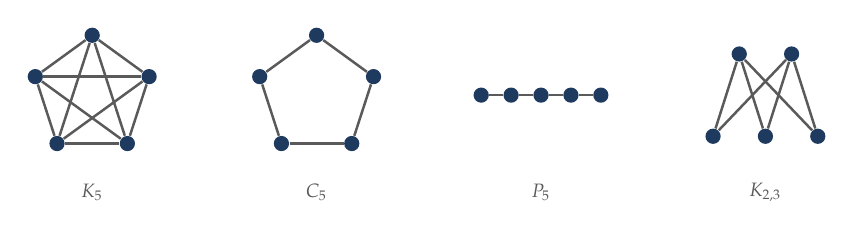
\begin{tikzpicture}[scale=0.95]
\begin{scope}
\foreach \i in {0,...,4} \node[knoten] (k\i) at (90+72*\i:0.8) {};
\foreach \i/\j in {0/1,0/2,0/3,0/4,1/2,1/3,1/4,2/3,2/4,3/4} \draw[kante] (k\i) -- (k\j);
\node[font=\scriptsize, color=grau] at (0,-1.3) {$K_5$};
\end{scope}
\begin{scope}[xshift=3.0cm]
\foreach \i in {0,...,4} \node[knoten] (c\i) at (90+72*\i:0.8) {};
\foreach \i/\j in {0/1,1/2,2/3,3/4,4/0} \draw[kante] (c\i) -- (c\j);
\node[font=\scriptsize, color=grau] at (0,-1.3) {$C_5$};
\end{scope}
\begin{scope}[xshift=6.0cm]
\foreach \i in {0,...,4} \node[knoten] (p\i) at (-0.8+0.4*\i,0) {};
\foreach \i/\j in {0/1,1/2,2/3,3/4} \draw[kante] (p\i) -- (p\j);
\node[font=\scriptsize, color=grau] at (0,-1.3) {$P_5$};
\end{scope}
\begin{scope}[xshift=9.0cm]
\foreach \i in {0,1} \node[knoten] (u\i) at (-0.35+0.7*\i,0.55) {};
\foreach \i in {0,1,2} \node[knoten] (w\i) at (-0.7+0.7*\i,-0.55) {};
\foreach \i in {0,1} \foreach \j in {0,1,2} \draw[kante] (u\i) -- (w\j);
\node[font=\scriptsize, color=grau] at (0,-1.3) {$K_{2,3}$};
\end{scope}
\end{tikzpicture}
\end{center}

\begin{center}
{\small
\renewcommand{\arraystretch}{1.45}
\begin{tabular}{@{}P{1.6cm}P{3.2cm}P{1.5cm}P{2.0cm}@{}}
\toprule
\textbf{Zeichen} & \textbf{Name} & \textbf{Ecken} & \textbf{Kanten}\\
\midrule
$K_n$ & vollständiger Graph & $n$ & $\binom{n}{2}$\\
$P_n$ & Weg & $n$ & $n-1$\\
$C_n$ & Kreis ($n \ge 3$) & $n$ & $n$\\
$K_{r,s}$ & vollständig bipartit & $r+s$ & $r \cdot s$\\
$Q_d$ & Würfelgraph & $2^d$ & $d \cdot 2^{d-1}$\\
\bottomrule
\end{tabular}}
\end{center}

\begin{center}
\begin{minipage}{0.88\textwidth}
\kursiv{Im $K_n$ ist jede Ecke mit jeder anderen verbunden --- er hat die größtmögliche Kantenzahl. Im $K_{r,s}$ zerfallen die Ecken in zwei Gruppen der Größen $r$ und $s$; jede Ecke der einen Gruppe ist mit jeder der anderen verbunden, innerhalb einer Gruppe gibt es keine Kante.}
\end{minipage}
\end{center}
\end{merksatz}

\begin{merksatz}
\boxtitel{Der Petersen-Graph --- der berühmteste Einzelgänger}
\begin{center}
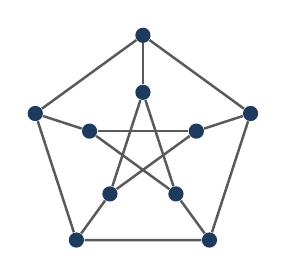
\begin{tikzpicture}[scale=1.15]
\foreach \i in {0,...,4} {
  \node[knoten] (a\i) at (90+72*\i:1.25) {};
  \node[knoten] (b\i) at (90+72*\i:0.62) {};
  \draw[kante] (a\i) -- (b\i);
}
\foreach \i/\j in {0/1,1/2,2/3,3/4,4/0} \draw[kante] (a\i) -- (a\j);
\foreach \i/\j in {0/2,1/3,2/4,3/0,4/1} \draw[kante] (b\i) -- (b\j);
\end{tikzpicture}
\end{center}

Zehn Ecken, fünfzehn Kanten, jede Ecke vom Grad $3$. Dieser Graph ist in der Graphentheorie das, was das Gegenbeispiel in der Analysis ist: Er widerlegt eine erstaunliche Zahl plausibler Vermutungen. Sie werden ihm in den Kapiteln 7, 9 und 13 wiederbegegnen.
\end{merksatz}

\section{Teilgraphen und das Komplement}

\begin{definition}
\boxtitelm{Definition 1.6 --- Teilgraph, induzierter Teilgraph, Komplement}
Sei $G = (V,E)$ ein Graph.
\begin{itemize}[leftmargin=1.4em, itemsep=4pt]
\item Ein \Begriff{Teilgraph} von $G$ ist ein Graph $H = (V', E')$ mit $V' \subseteq V$ und $E' \subseteq E$, wobei jede Kante aus $E'$ beide Endecken in $V'$ haben muss.
\item Für $S \subseteq V$ heißt der Graph mit Eckenmenge $S$ und \kursiv{allen} Kanten aus $E$, die beide Enden in $S$ haben, der von $S$ \Begriff{induzierte Teilgraph}; Zeichen $G[S]$.
\item Das \Begriff{Komplement} $\overline{G}$ hat dieselbe Eckenmenge $V$, und $\{u,v\}$ ist genau dann Kante von $\overline{G}$, wenn $\{u,v\}$ \kursiv{keine} Kante von $G$ ist.
\end{itemize}
\end{definition}

\begin{warnung}
\boxtitelr{Teilgraph und induzierter Teilgraph sind nicht dasselbe}
Beim Teilgraphen \kursiv{darf} man Kanten weglassen. Beim induzierten Teilgraphen \kursiv{muss} man alle nehmen, die zwischen den gewählten Ecken verlaufen.

\begin{center}
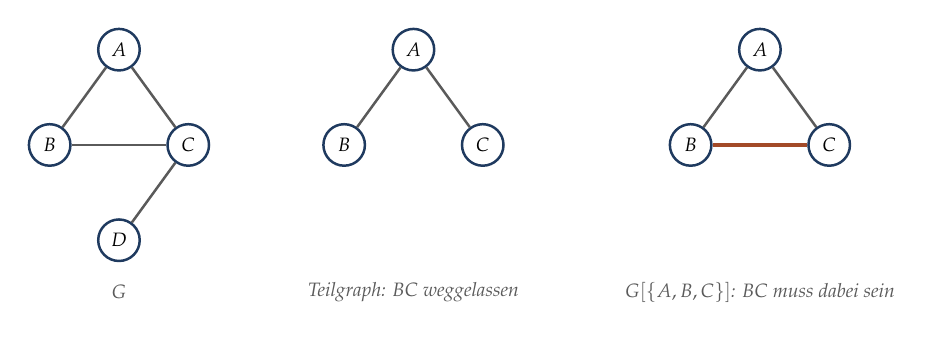
\begin{tikzpicture}[scale=1.1]
\begin{scope}
\node[knotenb] (A) at (0,0.8) {$A$};
\node[knotenb] (B) at (-0.8,-0.3) {$B$};
\node[knotenb] (C) at (0.8,-0.3) {$C$};
\node[knotenb] (D) at (0,-1.4) {$D$};
\draw[kante] (A) -- (B); \draw[kante] (A) -- (C);
\draw[kante] (B) -- (C); \draw[kante] (C) -- (D);
\node[font=\scriptsize\itshape, color=grau] at (0,-2.0) {$G$};
\end{scope}
\begin{scope}[xshift=3.4cm]
\node[knotenb] (A2) at (0,0.8) {$A$};
\node[knotenb] (B2) at (-0.8,-0.3) {$B$};
\node[knotenb] (C2) at (0.8,-0.3) {$C$};
\draw[kante] (A2) -- (B2); \draw[kante] (A2) -- (C2);
\node[font=\scriptsize\itshape, color=grau] at (0,-2.0) {Teilgraph: $BC$ weggelassen};
\end{scope}
\begin{scope}[xshift=7.4cm]
\node[knotenb] (A3) at (0,0.8) {$A$};
\node[knotenb] (B3) at (-0.8,-0.3) {$B$};
\node[knotenb] (C3) at (0.8,-0.3) {$C$};
\draw[kante] (A3) -- (B3); \draw[kante] (A3) -- (C3);
\draw[kanted] (B3) -- (C3);
\node[font=\scriptsize\itshape, color=grau] at (0,-2.0) {$G[\{A,B,C\}]$: $BC$ muss dabei sein};
\end{scope}
\end{tikzpicture}
\end{center}

\begin{center}
\begin{minipage}{0.88\textwidth}
\kursiv{Der Unterschied ist folgenreich. \enquote{$G$ enthält ein Dreieck als Teilgraph} und \enquote{$G$ enthält ein Dreieck als induzierten Teilgraph} sind verschiedene Aussagen --- die zweite verlangt zusätzlich, dass keine weitere Kante zwischen den drei Ecken fehlt. In Kapitel 13 hängt ein ganzer Satz an dieser Unterscheidung.}
\end{minipage}
\end{center}
\end{warnung}

\section{Isomorphie: Wann sind zwei Graphen derselbe?}

Wir kehren zur ersten Warnung des Vorworts zurück. Dieselbe Struktur kann sehr verschieden aussehen. Was heißt dann \enquote{derselbe Graph}?

\begin{merksatz}
\boxtitel{Warum \enquote{sieht gleich aus} keine Definition sein kann}
\begin{center}
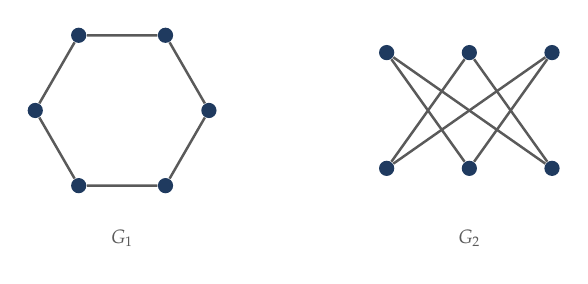
\begin{tikzpicture}[scale=1.05]
\begin{scope}
\foreach \i in {0,...,5} \node[knoten] (x\i) at (60*\i:1.05) {};
\foreach \i/\j in {0/1,1/2,2/3,3/4,4/5,5/0} \draw[kante] (x\i) -- (x\j);
\node[font=\scriptsize\itshape, color=grau] at (0,-1.55) {$G_1$};
\end{scope}
\begin{scope}[xshift=4.2cm]
\node[knoten] (y0) at (-1.0,0.7) {};
\node[knoten] (y1) at (0,0.7) {};
\node[knoten] (y2) at (1.0,0.7) {};
\node[knoten] (y3) at (-1.0,-0.7) {};
\node[knoten] (y4) at (0,-0.7) {};
\node[knoten] (y5) at (1.0,-0.7) {};
\draw[kante] (y0) -- (y4); \draw[kante] (y4) -- (y2);
\draw[kante] (y2) -- (y3); \draw[kante] (y3) -- (y1);
\draw[kante] (y1) -- (y5); \draw[kante] (y5) -- (y0);
\node[font=\scriptsize\itshape, color=grau] at (0,-1.55) {$G_2$};
\end{scope}
\end{tikzpicture}
\end{center}

Diese beiden Bilder sehen verschieden aus. Beide zeigen aber sechs Ecken, die zu einem einzigen geschlossenen Rundgang verbunden sind --- also den $C_6$. Ob Linien sich kreuzen, hängt vom Zeichnen ab, nicht vom Graphen.

Eine Definition, die \enquote{sieht gleich aus} zur Grundlage macht, wäre also unbrauchbar. Wir brauchen etwas, das nur von $V$ und $E$ spricht.
\end{merksatz}

\begin{definition}
\boxtitelm{Definition 1.7 --- Isomorphie}
Zwei Graphen $G = (V,E)$ und $H = (W,F)$ heißen \Begriff{isomorph}, geschrieben $G \cong H$, wenn es eine Abbildung
\[ \varphi : V \longrightarrow W \]
gibt mit den beiden Eigenschaften:
\begin{itemize}[leftmargin=1.4em, itemsep=3pt]
\item $\varphi$ ist \Begriff{bijektiv} --- jede Ecke von $H$ wird von genau einer Ecke von $G$ getroffen;
\item für alle $u, v \in V$ gilt: $\{u,v\} \in E \iff \{\varphi(u), \varphi(v)\} \in F$.
\end{itemize}
Eine solche Abbildung $\varphi$ heißt \Begriff{Isomorphismus}.
\end{definition}

\begin{merksatz}
\boxtitel{Was die zweite Bedingung wirklich verlangt}
Das Zeichen $\iff$ heißt \enquote{genau dann, wenn} und steht für \kursiv{zwei} Forderungen auf einmal:

\begin{center}
\renewcommand{\arraystretch}{1.5}
\begin{tabular}{@{}P{1.8cm}P{6.6cm}@{}}
\toprule
$\Longrightarrow$ & Wo in $G$ eine Kante ist, ist auch in $H$ eine --- \kursiv{keine Kante geht verloren}.\\
$\Longleftarrow$ & Wo in $G$ keine Kante ist, ist auch in $H$ keine --- \kursiv{keine Kante kommt hinzu}.\\
\bottomrule
\end{tabular}
\end{center}

\begin{center}
\begin{minipage}{0.88\textwidth}
\kursiv{Die zweite Richtung wird gern vergessen. Ohne sie könnte man jeden Graphen in den vollständigen $K_n$ \enquote{abbilden}, und der Begriff wäre wertlos.}
\end{minipage}
\end{center}
\end{merksatz}

\begin{merksatz}
\boxtitel{Ein Isomorphismus, vollständig hingeschrieben}
Wir zeigen $G_1 \cong G_2$ für die beiden Bilder oben. Nummerieren wir:

$G_1$: Ecken $1,2,3,4,5,6$ im Kreis, Kanten $12, 23, 34, 45, 56, 61$.

$G_2$: Ecken $y_0, \ldots, y_5$, Kanten $y_0y_4$, $y_4y_2$, $y_2y_3$, $y_3y_1$, $y_1y_5$, $y_5y_0$.

\schritt{Die Idee}
Wir laufen den Rundgang von $G_2$ ab und ordnen ihm die Nummern von $G_1$ der Reihe nach zu.

Der Rundgang von $G_2$ lautet: $y_0 \to y_4 \to y_2 \to y_3 \to y_1 \to y_5 \to y_0$.

\schritt{Die Abbildung}
\[ \varphi(1) = y_0,\quad \varphi(2) = y_4,\quad \varphi(3) = y_2,\quad \varphi(4) = y_3,\quad \varphi(5) = y_1,\quad \varphi(6) = y_5 \]

\schritt{Prüfung der Bijektivität}
Die sechs Bildwerte $y_0, y_4, y_2, y_3, y_1, y_5$ sind paarweise verschieden und erschöpfen alle sechs Ecken von $G_2$. Also bijektiv.

\schritt{Prüfung der Kantenbedingung --- Richtung $\Longrightarrow$}
\begin{center}
{\small
\renewcommand{\arraystretch}{1.35}
\begin{tabular}{@{}P{1.6cm}P{2.4cm}P{2.6cm}@{}}
\toprule
\textbf{Kante in $G_1$} & \textbf{Bild} & \textbf{In $G_2$?}\\
\midrule
$\{1,2\}$ & $\{y_0, y_4\}$ & ja\\
$\{2,3\}$ & $\{y_4, y_2\}$ & ja\\
$\{3,4\}$ & $\{y_2, y_3\}$ & ja\\
$\{4,5\}$ & $\{y_3, y_1\}$ & ja\\
$\{5,6\}$ & $\{y_1, y_5\}$ & ja\\
$\{6,1\}$ & $\{y_5, y_0\}$ & ja\\
\bottomrule
\end{tabular}}
\end{center}

\schritt{Prüfung der Kantenbedingung --- Richtung $\Longleftarrow$}
Hier kann man sich Arbeit sparen. Beide Graphen haben genau sechs Kanten. Die sechs Kanten von $G_1$ wurden auf sechs \kursiv{verschiedene} Kanten von $G_2$ abgebildet (verschieden, weil $\varphi$ bijektiv ist). Also sind damit \kursiv{alle} Kanten von $G_2$ getroffen, und es bleibt keine übrig, die ein Bild eines Nicht-Kanten-Paares sein könnte. $\blacksquare$

\begin{center}
\begin{minipage}{0.86\textwidth}
\kursiv{Dieses Abkürzungsargument funktioniert immer, wenn beide Graphen \kursiv{gleich viele} Kanten haben: Dann genügt die Richtung $\Longrightarrow$. Haben sie verschieden viele, sind sie ohnehin nicht isomorph.}
\end{minipage}
\end{center}
\end{merksatz}

\subsection*{Wie man Nicht-Isomorphie zeigt}

Um $G \cong H$ zu zeigen, gibt man einen Isomorphismus an. Um $G \not\cong H$ zu zeigen, müsste man \kursiv{alle} Abbildungen ausschließen --- bei $n$ Ecken sind das $n!$ Stück. Für $n = 10$ wären das $3\,628\,800$. Das ist kein gangbarer Weg.

\begin{definition}
\boxtitelm{Definition 1.8 --- Invariante}
Eine \Begriff{Invariante} ist eine Eigenschaft oder Kennzahl eines Graphen, die bei isomorphen Graphen übereinstimmt.
\end{definition}

\begin{merksatz}
\boxtitel{Die Standardinvarianten --- in der Reihenfolge, in der man sie prüft}
\begin{center}
{\small
\renewcommand{\arraystretch}{1.45}
\begin{tabular}{@{}P{0.8cm}P{3.4cm}P{4.0cm}@{}}
\toprule
& \textbf{Invariante} & \textbf{Aufwand}\\
\midrule
1 & Eckenzahl $n$ & sofort\\
2 & Kantenzahl $m$ & sofort\\
3 & Gradfolge & schnell\\
4 & Zahl der Dreiecke & mäßig\\
5 & Länge des kürzesten Kreises & mäßig\\
6 & Zusammenhang (Kapitel 2) & schnell\\
7 & Eigenwerte (Kapitel 14) & aufwendig\\
\bottomrule
\end{tabular}}
\end{center}

\begin{center}
\begin{minipage}{0.88\textwidth}
\kursiv{Man prüft von oben nach unten und hört auf, sobald eine Invariante verschieden ausfällt --- dann sind die Graphen nicht isomorph, und man ist fertig.}
\end{minipage}
\end{center}
\end{merksatz}

\begin{warnung}
\boxtitelr{Gleiche Invarianten beweisen gar nichts}
Invarianten können Nicht-Isomorphie beweisen. Sie können Isomorphie \kursiv{nie} beweisen.

\begin{center}
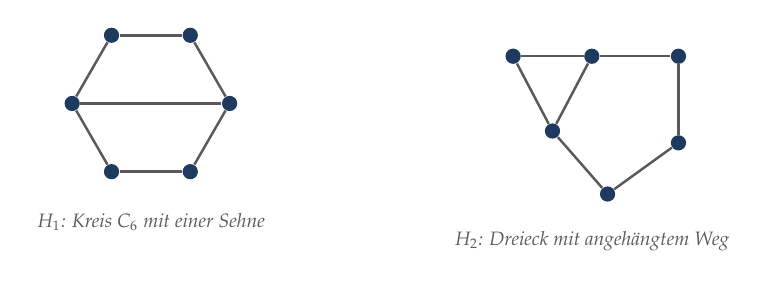
\begin{tikzpicture}[scale=1.0]
\begin{scope}
\foreach \i in {0,...,5} \node[knoten] (u\i) at (60*\i:1.0) {};
\foreach \i/\j in {0/1,1/2,2/3,3/4,4/5,5/0,0/3} \draw[kante] (u\i) -- (u\j);
\node[font=\scriptsize\itshape, color=grau] at (0,-1.5) {$H_1$: Kreis $C_6$ mit einer Sehne};
\end{scope}
\begin{scope}[xshift=5.6cm]
\node[knoten] (v0) at (-1.0,0.6) {};
\node[knoten] (v1) at (0,0.6) {};
\node[knoten] (v2) at (-0.5,-0.35) {};
\node[knoten] (v3) at (1.1,0.6) {};
\node[knoten] (v4) at (1.1,-0.5) {};
\node[knoten] (v5) at (0.2,-1.15) {};
\draw[kante] (v0) -- (v1); \draw[kante] (v1) -- (v2); \draw[kante] (v2) -- (v0);
\draw[kante] (v1) -- (v3); \draw[kante] (v3) -- (v4); \draw[kante] (v4) -- (v5);
\draw[kante] (v5) -- (v2);
\node[font=\scriptsize\itshape, color=grau] at (0,-1.75) {$H_2$: Dreieck mit angehängtem Weg};
\end{scope}
\end{tikzpicture}
\end{center}

Beide haben $n = 6$, $m = 7$ und die Gradfolge $(3,3,2,2,2,2)$ --- drei Invarianten stimmen überein. Trotzdem sind sie nicht isomorph: $H_2$ enthält ein Dreieck (drei paarweise benachbarte Ecken), $H_1$ nicht. Die vierte Invariante entscheidet.

\begin{center}
\begin{minipage}{0.88\textwidth}
\kursiv{Es gibt \kursiv{keine} bekannte Liste von leicht berechenbaren Invarianten, die Isomorphie vollständig entscheidet. Wie schwer das Problem wirklich ist, gehört zu den bemerkenswertesten offenen Fragen des Gebiets --- Kapitel 15 kommt darauf zurück.}
\end{minipage}
\end{center}
\end{warnung}

\section{Übungsaufgaben}

\begin{aufgabe}
\boxtitel{Aufgabe 1.1 --- Grade und Kanten}
Ein Graph hat $12$ Ecken. Sieben davon haben Grad $3$, die übrigen haben Grad $k$. Der Graph hat $30$ Kanten. Bestimmen Sie $k$.

\loesung
\schritt{Schritt 1 --- Was gegeben ist}
$n = 12$, davon $7$ Ecken vom Grad $3$ und $12 - 7 = 5$ Ecken vom Grad $k$. Weiter $m = 30$.

\schritt{Schritt 2 --- Handschlaglemma ansetzen}
Nach Satz 1.3 gilt $\sum_{v} \deg(v) = 2m$. Die linke Seite zerlegen wir nach den beiden Sorten von Ecken:
\[ \underbrace{7 \cdot 3}_{\text{die sieben}} + \underbrace{5 \cdot k}_{\text{die fünf}} = 2 \cdot 30 \]

\schritt{Schritt 3 --- Auflösen}
\begin{align*}
21 + 5k &= 60 \\
5k &= 60 - 21 = 39 \\
k &= \frac{39}{5} = 7{,}8
\end{align*}

\schritt{Schritt 4 --- Das Ergebnis deuten}
$k$ müsste $7{,}8$ sein. Ein Grad ist aber die Anzahl von Nachbarn, also eine \kursiv{ganze} Zahl. Es gibt daher \textbf{keinen} solchen Graphen.

\schritt{Probe}
Gegenrechnung mit $k = 7$: Gradsumme $21 + 35 = 56 = 2m$, also $m = 28$. Mit $k = 8$: $21 + 40 = 61$ --- ungerade, nach Satz 1.4 unmöglich. Die geforderten $30$ Kanten liegen zwischen diesen Fällen und sind nicht erreichbar.

\begin{center}
\begin{minipage}{0.86\textwidth}
\kursiv{Aufgaben, deren Antwort \enquote{gibt es nicht} lautet, sind in der Graphentheorie häufig. Wer die Rechnung durchführt und bei $7{,}8$ stutzt, hat richtig gearbeitet --- wer $k \approx 8$ hinschreibt, hat den Kern verfehlt.}
\end{minipage}
\end{center}
\end{aufgabe}

\begin{aufgabe}
\boxtitel{Aufgabe 1.2 --- Das Komplement}
Sei $G$ ein Graph mit $n = 6$ Ecken und der Gradfolge $(4,3,3,2,2,2)$. Bestimmen Sie die Gradfolge des Komplements $\overline{G}$ und die Kantenzahl beider Graphen.

\loesung
\schritt{Schritt 1 --- Der Grundgedanke}
Im Komplement ist eine Ecke $v$ genau mit den Ecken benachbart, mit denen sie in $G$ \kursiv{nicht} benachbart war. Es gibt $n - 1 = 5$ andere Ecken. Von diesen sind $\deg_G(v)$ Stück Nachbarn in $G$, der Rest ist Nachbar in $\overline{G}$:
\[ \deg_{\overline{G}}(v) = (n-1) - \deg_G(v) = 5 - \deg_G(v) . \]

\schritt{Schritt 2 --- Einsetzen}
\begin{center}
\renewcommand{\arraystretch}{1.4}
\begin{tabular}{@{}P{2.6cm}P{5.2cm}@{}}
\toprule
$\deg_G$ & $4,\ 3,\ 3,\ 2,\ 2,\ 2$\\
$5 - \deg_G$ & $1,\ 2,\ 2,\ 3,\ 3,\ 3$\\
\bottomrule
\end{tabular}
\end{center}
Absteigend sortiert: $\deg_{\overline{G}} = (3,3,3,2,2,1)$.

\schritt{Schritt 3 --- Die Kantenzahlen}
Für $G$ mit Satz 1.3:
\[ m_G = \frac{4+3+3+2+2+2}{2} = \frac{16}{2} = 8 . \]
Für $\overline{G}$:
\[ m_{\overline{G}} = \frac{3+3+3+2+2+1}{2} = \frac{14}{2} = 7 . \]

\schritt{Probe}
Jedes der $\binom{6}{2} = 15$ möglichen Paare ist entweder in $G$ oder in $\overline{G}$ eine Kante, nie in beiden und nie in keinem. Also muss $m_G + m_{\overline{G}} = 15$ gelten:
\[ 8 + 7 = 15 . \quad \checkmark \]
\end{aufgabe}

\begin{aufgabe}
\boxtitel{Aufgabe 1.3 --- Isomorph oder nicht?}
Sind die folgenden beiden Graphen isomorph?

\begin{center}
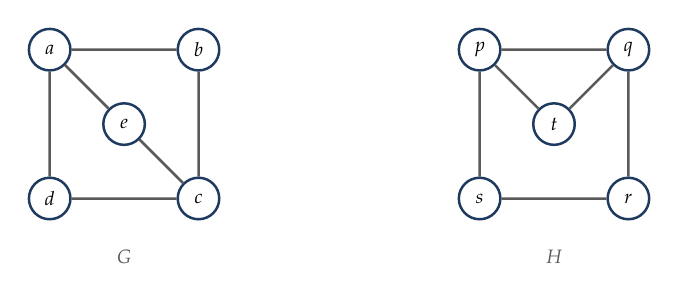
\begin{tikzpicture}[scale=1.05]
\begin{scope}
\node[knotenb] (a1) at (-0.9,0.9) {$a$};
\node[knotenb] (a2) at (0.9,0.9) {$b$};
\node[knotenb] (a3) at (0.9,-0.9) {$c$};
\node[knotenb] (a4) at (-0.9,-0.9) {$d$};
\node[knotenb] (a5) at (0,0) {$e$};
\draw[kante] (a1) -- (a2); \draw[kante] (a2) -- (a3);
\draw[kante] (a3) -- (a4); \draw[kante] (a4) -- (a1);
\draw[kante] (a5) -- (a1); \draw[kante] (a5) -- (a3);
\node[font=\scriptsize\itshape, color=grau] at (0,-1.6) {$G$};
\end{scope}
\begin{scope}[xshift=5.2cm]
\node[knotenb] (b1) at (-0.9,0.9) {$p$};
\node[knotenb] (b2) at (0.9,0.9) {$q$};
\node[knotenb] (b3) at (0.9,-0.9) {$r$};
\node[knotenb] (b4) at (-0.9,-0.9) {$s$};
\node[knotenb] (b5) at (0,0) {$t$};
\draw[kante] (b1) -- (b2); \draw[kante] (b2) -- (b3);
\draw[kante] (b3) -- (b4); \draw[kante] (b4) -- (b1);
\draw[kante] (b5) -- (b1); \draw[kante] (b5) -- (b2);
\node[font=\scriptsize\itshape, color=grau] at (0,-1.6) {$H$};
\end{scope}
\end{tikzpicture}
\end{center}

\loesung
\schritt{Schritt 1 --- Die schnellen Invarianten}
Beide haben $n = 5$ und $m = 6$. Kein Ausschluss.

\schritt{Schritt 2 --- Die Gradfolgen}
In $G$: $\deg(a) = 3$ (Nachbarn $b, d, e$), $\deg(b) = 2$, $\deg(c) = 3$ (Nachbarn $b, d, e$), $\deg(d) = 2$, $\deg(e) = 2$. Gradfolge $(3,3,2,2,2)$.

In $H$: $\deg(p) = 3$ (Nachbarn $q, s, t$), $\deg(q) = 3$ (Nachbarn $p, r, t$), $\deg(r) = 2$, $\deg(s) = 2$, $\deg(t) = 2$. Gradfolge $(3,3,2,2,2)$.

Gleich. Kein Ausschluss.

\schritt{Schritt 3 --- Die nächste Invariante: Sind die Ecken vom Grad 3 benachbart?}
Das ist eine Invariante, denn ein Isomorphismus bildet Ecken vom Grad $3$ auf Ecken vom Grad $3$ ab und erhält Kanten.

In $G$ sind die Ecken vom Grad $3$ gerade $a$ und $c$. Ist $\{a,c\}$ eine Kante? Die Kantenliste von $G$ lautet $ab, bc, cd, da, ea, ec$. Die Kante $ac$ kommt nicht vor --- \textbf{nicht benachbart}.

In $H$ sind die Ecken vom Grad $3$ gerade $p$ und $q$. Die Kantenliste lautet $pq, qr, rs, sp, tp, tq$. Die Kante $pq$ kommt vor --- \textbf{benachbart}.

\schritt{Schritt 4 --- Schluss}
Die Invariante unterscheidet die beiden Graphen. Also gilt $G \not\cong H$.

\schritt{Kontrolle über eine zweite Invariante}
$H$ enthält das Dreieck $p, q, t$ (denn $pq$, $qt$ und $tp$ sind Kanten). Enthält $G$ ein Dreieck? Die Ecke $e$ hat Nachbarn $a$ und $c$, und $ac$ ist keine Kante --- kein Dreieck über $e$. Die Ecke $b$ hat Nachbarn $a$ und $c$, ebenso. Die Ecke $d$ hat Nachbarn $c$ und $a$, ebenso. $G$ ist dreiecksfrei. Beide Wege führen zum selben Ergebnis. $\checkmark$
\end{aufgabe}

\begin{aufgabe}
\boxtitel{Aufgabe 1.4 --- Gibt es einen Graphen zur Gradfolge $(4,4,3,3,2,2)$?}
Entscheiden Sie mit dem Verfahren von Havel und Hakimi, und geben Sie gegebenenfalls einen Graphen an.

\loesung
\schritt{Schritt 0 --- Das Verfahren, zuerst erklärt}
Der Gedanke: Die Ecke mit dem größten Grad $d$ muss $d$ Nachbarn haben. Man darf annehmen, dass sie mit den $d$ Ecken der \kursiv{nächstgrößten} Grade verbunden ist. Dann streicht man diese Ecke und senkt die Grade ihrer $d$ Nachbarn um $1$. Bleibt eine gültige Folge übrig, war die ursprüngliche gültig.

\schritt{Schritt 1 --- Erste Prüfung}
Summe $4+4+3+3+2+2 = 18$, gerade. Alle Werte $\le n-1 = 5$. Beide Bedingungen erfüllt.

\schritt{Schritt 2 --- Erster Durchgang}
Folge: $(4,4,3,3,2,2)$. Wir nehmen die erste $4$ weg und ziehen von den nächsten vier Zahlen je $1$ ab:
\[ \underline{4} \mid 4,\ 3,\ 3,\ 2 \mid 2 \;\longrightarrow\; 3,\ 2,\ 2,\ 1 \mid 2 \]
Neue Folge, sortiert: $(3,2,2,2,1)$.

\schritt{Schritt 3 --- Zweiter Durchgang}
\[ \underline{3} \mid 2,\ 2,\ 2 \mid 1 \;\longrightarrow\; 1,\ 1,\ 1 \mid 1 \]
Neue Folge, sortiert: $(1,1,1,1)$.

\schritt{Schritt 4 --- Dritter Durchgang}
\[ \underline{1} \mid 1 \mid 1,\ 1 \;\longrightarrow\; 0 \mid 1,\ 1 \]
Neue Folge, sortiert: $(1,1,0)$.

\schritt{Schritt 5 --- Vierter Durchgang}
\[ \underline{1} \mid 1 \mid 0 \;\longrightarrow\; 0 \mid 0 \]
Neue Folge: $(0,0)$. Das ist die Gradfolge zweier isolierter Ecken --- offensichtlich möglich. Das Verfahren endet erfolgreich.

\schritt{Schritt 6 --- Den Graphen zurückbauen}
Wir vergeben Namen $v_1, \ldots, v_6$ für die Grade $4,4,3,3,2,2$ und lesen die Durchgänge rückwärts als Kantenliste:
\begin{center}
\renewcommand{\arraystretch}{1.4}
\begin{tabular}{@{}P{2.0cm}P{5.4cm}@{}}
\toprule
Durchgang 1 & $v_1 v_2$, $v_1 v_3$, $v_1 v_4$, $v_1 v_5$\\
Durchgang 2 & $v_2 v_3$, $v_2 v_4$, $v_2 v_6$\\
Durchgang 3 & $v_3 v_4$\\
Durchgang 4 & $v_5 v_6$\\
\bottomrule
\end{tabular}
\end{center}

\schritt{Schritt 7 --- Probe durch Nachzählen der Grade}
\begin{center}
\renewcommand{\arraystretch}{1.4}
\begin{tabular}{@{}P{1.2cm}P{4.0cm}P{1.4cm}P{1.4cm}@{}}
\toprule
\textbf{Ecke} & \textbf{Nachbarn} & \textbf{Grad} & \textbf{Soll}\\
\midrule
$v_1$ & $v_2, v_3, v_4, v_5$ & $4$ & $4$ \checkmark\\
$v_2$ & $v_1, v_3, v_4, v_6$ & $4$ & $4$ \checkmark\\
$v_3$ & $v_1, v_2, v_4$ & $3$ & $3$ \checkmark\\
$v_4$ & $v_1, v_2, v_3$ & $3$ & $3$ \checkmark\\
$v_5$ & $v_1, v_6$ & $2$ & $2$ \checkmark\\
$v_6$ & $v_2, v_5$ & $2$ & $2$ \checkmark\\
\bottomrule
\end{tabular}
\end{center}
Kantenzahl: $4 + 3 + 1 + 1 = 9 = \tfrac{18}{2}$. \checkmark

\schritt{Und als Bild}
\begin{center}
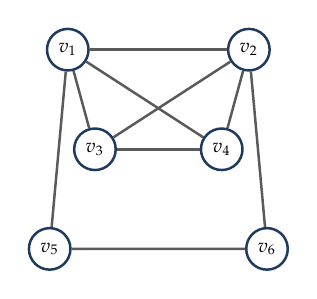
\begin{tikzpicture}[scale=1.15]
\node[knotenb] (v1) at (-1.0,0.9) {$v_1$};
\node[knotenb] (v2) at (1.0,0.9) {$v_2$};
\node[knotenb] (v3) at (-0.7,-0.2) {$v_3$};
\node[knotenb] (v4) at (0.7,-0.2) {$v_4$};
\node[knotenb] (v5) at (-1.2,-1.3) {$v_5$};
\node[knotenb] (v6) at (1.2,-1.3) {$v_6$};
\draw[kante] (v1) -- (v2); \draw[kante] (v1) -- (v3);
\draw[kante] (v1) -- (v4); \draw[kante] (v1) -- (v5);
\draw[kante] (v2) -- (v3); \draw[kante] (v2) -- (v4);
\draw[kante] (v2) -- (v6); \draw[kante] (v3) -- (v4);
\draw[kante] (v5) -- (v6);
\end{tikzpicture}
\end{center}
\end{aufgabe}

\begin{aufgabe}
\boxtitel{Aufgabe 1.5 --- Eine Aussage über alle Graphen}
Zeigen Sie: In jedem Graphen mit mindestens zwei Ecken gibt es zwei Ecken mit demselben Grad.

\loesung
\schritt{Schritt 1 --- Wiedererkennen}
Das ist die Aussage aus dem Vorwort, jetzt in der Fachsprache. Wir führen sie noch einmal, aber mit dem Begriff, der den Beweis kürzer macht.

\schritt{Schritt 2 --- Die möglichen Grade}
In einem Graphen mit $n$ Ecken gilt für jede Ecke $0 \le \deg(v) \le n-1$. Es gibt also $n$ mögliche Werte für $n$ Ecken.

\schritt{Schritt 3 --- Annahme für einen Widerspruchsbeweis}
Angenommen, alle Grade sind verschieden. Dann kommt jeder der Werte $0, 1, \ldots, n-1$ genau einmal vor.

\schritt{Schritt 4 --- Zwei besondere Ecken}
Es gibt eine Ecke $x$ mit $\deg(x) = 0$ und eine Ecke $y$ mit $\deg(y) = n-1$. Wegen $n \ge 2$ ist $0 \neq n-1$, also $x \neq y$.

\schritt{Schritt 5 --- Der Widerspruch}
$\deg(y) = n-1$ bedeutet: $y$ ist mit allen $n-1$ übrigen Ecken benachbart. Da $x \neq y$, gehört $x$ zu diesen übrigen. Also ist $\{x,y\} \in E$.

Damit ist $x \in N(y)$ und ebenso $y \in N(x)$ --- denn $\{x,y\} = \{y,x\}$ ist dieselbe Kante. Also $\deg(x) \ge 1$, im Widerspruch zu $\deg(x) = 0$.

\schritt{Schritt 6 --- Schluss}
Die Annahme ist falsch. Es gibt also zwei Ecken gleichen Grades. $\blacksquare$

\schritt{Nachbemerkung --- wo die Voraussetzung steckt}
Für $n = 1$ ist die Aussage falsch: Ein einzelner Punkt hat genau einen Grad, nämlich $0$, und es gibt keine zwei Ecken. Die Voraussetzung $n \ge 2$ wurde in Schritt 4 gebraucht, um $x \neq y$ zu sichern.
\end{aufgabe}

\begin{geschichte}
\boxtitelg{Wie das Wort \enquote{Graph} in die Mathematik kam}
Euler löste 1736 das Königsberger Problem, ohne das Wort zu benutzen; er sprach von \kursiv{geometria situs}, der Geometrie der Lage. Sein Aufsatz \kursiv{Solutio problematis ad geometriam situs pertinentis} gilt heute als Geburtsurkunde des Gebiets --- und ist zugleich ein Musterbeispiel dafür, wie eine Fragestellung durch Weglassen des Unwesentlichen lösbar wird. Die Längen der Brücken, die Form der Insel, die Breite des Flusses: alles gestrichen.

Das Wort \enquote{Graph} führte \Person{James Joseph Sylvester} 1878 in einer Notiz in \kursiv{Nature} ein. Er entlehnte es der Chemie: Chemiker zeichneten damals Strukturformeln --- Atome als Punkte, Bindungen als Striche --- und nannten diese Bilder \kursiv{graphic notation}. Sylvester bemerkte, dass die Algebra der Invarianten mit diesen Diagrammen zusammenhängt.

Das erste Lehrbuch erschien erst 1936: \kursiv{Theorie der endlichen und unendlichen Graphen} von \Person{Dénes König}. Zwischen Euler und König liegen zweihundert Jahre, in denen das Gebiet aus lauter Einzelproblemen bestand --- dem Vierfarbenproblem, den Bäumen von Cayley, den Schaltkreisen von Kirchhoff. König war der Erste, der daraus ein Fach machte.
\end{geschichte}

\begin{forschung}
\boxtitelp{Wie groß sind die Graphen, über die heute geredet wird?}
Die Definition verlangt nur, dass $V$ endlich ist. In der Praxis reicht die Spanne weit.

\begin{center}
{\small
\renewcommand{\arraystretch}{1.42}
\begin{tabular}{@{}P{3.2cm}P{2.2cm}P{2.6cm}@{}}
\toprule
\textbf{Gegenstand} & \textbf{Ecken} & \textbf{Kanten}\\
\midrule
Petersen-Graph & $10$ & $15$\\
Kontaktnetz einer Station & $\sim 10^2$ & $\sim 10^3$\\
Straßennetz Deutschlands & $\sim 10^7$ & $\sim 10^7$\\
Konnektom der Fruchtfliege & $\sim 1{,}4 \cdot 10^5$ & $\sim 5 \cdot 10^7$\\
Weltweites Netz der Verweise & $> 10^{11}$ & $> 10^{12}$\\
\bottomrule
\end{tabular}}
\end{center}

\begin{center}
\begin{minipage}{0.88\textwidth}
\kursiv{Die vierte Zeile ist neu: Das vollständige Konnektom einer erwachsenen Fruchtfliege wurde 2024 veröffentlicht --- der erste vollständig kartierte Gehirngraph eines Tieres mit komplexem Verhalten. Was man daraus lernt, steht in Band 14 der Informatikreihe; dass man es überhaupt als Graphen aufschreibt, ist die Entscheidung aus Definition 1.1.}
\end{minipage}
\end{center}
\end{forschung}

\begin{merksatz}
\boxtitel{Was Sie jetzt können}
\begin{center}
\renewcommand{\arraystretch}{1.5}
\begin{tabular}{@{}P{3.2cm}P{5.4cm}@{}}
\toprule
\textbf{Begriff} & Graph als Paar $(V,E)$, Ecke, Kante, Ordnung, Größe\\
\textbf{Grad} & Nachbarschaft, Grad, Gradfolge, isolierte Ecke\\
\textbf{Satz 1.3} & Gradsumme $= 2m$, bewiesen durch Doppelzählung\\
\textbf{Satz 1.4} & Gerade Anzahl von Ecken ungeraden Grades\\
\textbf{Familien} & $K_n$, $P_n$, $C_n$, $K_{r,s}$, $Q_d$, Petersen\\
\textbf{Isomorphie} & Definition, Nachweis, Widerlegung durch Invarianten\\
\bottomrule
\end{tabular}
\end{center}

\begin{center}
\begin{minipage}{0.88\textwidth}
\kursiv{Im nächsten Kapitel geht es um die Frage, die im Hygienebeispiel offen blieb: Wann kann man von einer Ecke zu einer anderen gelangen, und wie zerfällt ein Graph in Teile, zwischen denen es keine Verbindung gibt?}
\end{minipage}
\end{center}
\end{merksatz}

\chapter{Wege, Kreise und Zusammenhang}

\section{Die Frage des Hygieneteams}

Aus Kapitel~1 ist eine Frage offengeblieben. Auf einer Station wurde ein Keim nachgewiesen; es liegt eine Liste von Kontakten vor. Gefragt war:

\begin{merksatz}
\boxtitel{Die Frage, aufgeteilt in ihre Bestandteile}
\begin{center}
\renewcommand{\arraystretch}{1.5}
\begin{tabular}{@{}P{1.0cm}P{7.4cm}@{}}
\toprule
(a) & Kann der Keim von Person $u$ überhaupt zu Person $v$ gelangt sein?\\
(b) & Über wie viele Zwischenschritte mindestens?\\
(c) & Zerfällt die Station in Gruppen ohne jeden Kontakt untereinander?\\
(d) & Gibt es eine einzelne Person, deren Isolierung die Station in zwei kontaktlose Hälften teilt?\\
\bottomrule
\end{tabular}
\end{center}
\end{merksatz}

Alle vier Fragen sind graphentheoretisch, und alle vier bekommen in diesem Kapitel eine Antwort. Frage (a) führt auf den Begriff des Zusammenhangs, (b) auf den Abstand, (c) auf die Zusammenhangskomponenten, (d) auf die Schnittecke.

Zuerst brauchen wir jedoch Ordnung in der Sprache. Das Vorwort hat gewarnt, dass gerade das Wort \enquote{Weg} in verschiedenen Büchern Verschiedenes bedeutet. Hier wird es festgelegt.

\section{Kantenzug, Weg, Kreis}

\begin{definition}
\boxtitelm{Definition 2.1 --- Kantenzug}
Sei $G = (V,E)$ ein Graph. Ein \Begriff{Kantenzug} von $u$ nach $v$ ist eine endliche Folge
\[ W = (v_0,\ v_1,\ v_2,\ \ldots,\ v_k) \]
von Ecken mit
\begin{itemize}[leftmargin=1.4em, itemsep=3pt]
\item $v_0 = u$ und $v_k = v$,
\item $\{v_{i-1}, v_i\} \in E$ für alle $i = 1, 2, \ldots, k$.
\end{itemize}
Die Zahl $k$ heißt die \Begriff{Länge} des Kantenzugs. Für $k = 0$ ist $W = (u)$ ein Kantenzug der Länge $0$ von $u$ nach $u$.
\end{definition}

\begin{merksatz}
\boxtitel{Was diese Definition erlaubt --- und was sie nicht sagt}
Die Definition verlangt nur eines: dass je zwei aufeinanderfolgende Ecken benachbart sind. Sie verbietet \kursiv{nicht}, dass eine Ecke mehrfach vorkommt, und sie verbietet nicht, dass eine Kante mehrfach benutzt wird.

\begin{center}
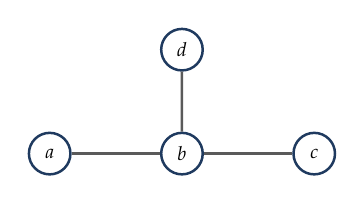
\begin{tikzpicture}[scale=1.2]
\node[knotenb] (a) at (0,0) {$a$};
\node[knotenb] (b) at (1.4,0) {$b$};
\node[knotenb] (c) at (2.8,0) {$c$};
\node[knotenb] (d) at (1.4,1.1) {$d$};
\draw[kante] (a) -- (b); \draw[kante] (b) -- (c);
\draw[kante] (b) -- (d);
\end{tikzpicture}
\end{center}

\begin{center}
{\small
\renewcommand{\arraystretch}{1.45}
\begin{tabular}{@{}P{3.2cm}P{1.4cm}P{3.6cm}@{}}
\toprule
\textbf{Folge} & \textbf{Länge} & \textbf{Zulässiger Kantenzug?}\\
\midrule
$(a,b,c)$ & $2$ & ja\\
$(a,b,d,b,c)$ & $4$ & ja --- $b$ zweimal, Kante $bd$ zweimal\\
$(a,b,a,b,c)$ & $4$ & ja --- Kante $ab$ dreimal\\
$(a,c)$ & --- & \textcolor{akzent}{\textbf{nein}} --- $\{a,c\} \notin E$\\
$(a)$ & $0$ & ja\\
\bottomrule
\end{tabular}}
\end{center}

\begin{center}
\begin{minipage}{0.88\textwidth}
\kursiv{Die Länge zählt \kursiv{Schritte}, nicht Ecken. Ein Kantenzug mit $k+1$ Eckeneinträgen hat Länge $k$. Diese Verschiebung um eins ist eine der häufigsten Fehlerquellen bei Rechnungen mit Kantenzügen.}
\end{minipage}
\end{center}
\end{merksatz}

\begin{definition}
\boxtitelm{Definition 2.2 --- Weg und Kreis}
Sei $W = (v_0, \ldots, v_k)$ ein Kantenzug.
\begin{itemize}[leftmargin=1.4em, itemsep=4pt]
\item $W$ heißt \Begriff{Weg}, wenn alle Ecken $v_0, v_1, \ldots, v_k$ paarweise verschieden sind.
\item $W$ heißt \Begriff{Kreis}, wenn $k \ge 3$ gilt, $v_0 = v_k$ ist und die Ecken $v_0, v_1, \ldots, v_{k-1}$ paarweise verschieden sind.
\end{itemize}
\end{definition}

\begin{warnung}
\boxtitelr{Warum beim Kreis $k \ge 3$ gefordert wird}
Ohne diese Bedingung wären zwei Gebilde \enquote{Kreise}, die keine sein sollen:

\begin{center}
\renewcommand{\arraystretch}{1.5}
\begin{tabular}{@{}P{1.5cm}P{2.6cm}P{4.2cm}@{}}
\toprule
$k = 1$ & $(v_0, v_0)$ & bräuchte die Kante $\{v_0,v_0\}$ --- gibt es nach Definition 1.1 nicht\\
$k = 2$ & $(u, v, u)$ & benutzt die Kante $\{u,v\}$ zweimal --- hin und zurück\\
\bottomrule
\end{tabular}
\end{center}

Der zweite Fall ist der eigentliche Grund für die Bedingung. Ein Hin und Zurück über dieselbe Kante ist kein Rundgang; nähme man ihn zu, so enthielte \kursiv{jeder} Graph mit mindestens einer Kante einen Kreis, und der Begriff wäre wertlos.

\begin{center}
\begin{minipage}{0.88\textwidth}
\kursiv{Der kürzestmögliche Kreis hat also Länge $3$ und heißt \Begriff{Dreieck}. Ein Graph ohne Kreise heißt \Begriff{kreisfrei} --- daraus wird in Kapitel~4 der Begriff des Baumes.}
\end{minipage}
\end{center}
\end{warnung}

\subsection*{Vom Kantenzug zum Weg}

Der folgende Hilfssatz sieht harmlos aus und wird in diesem Band ein Dutzend Mal gebraucht. Er erlaubt es, in Beweisen bequem mit Kantenzügen zu arbeiten und am Ende dennoch einen Weg zu haben.

\begin{merksatz}
\boxtitel{Lemma 2.3}
Gibt es in $G$ einen Kantenzug von $u$ nach $v$, so gibt es auch einen \kursiv{Weg} von $u$ nach $v$.
\end{merksatz}

\begin{merksatz}
\boxtitel{Beweis --- durch Verkürzen}
\schritt{Schritt 1 --- Die richtige Auswahl treffen}
Es gibt nach Voraussetzung mindestens einen Kantenzug von $u$ nach $v$. Unter allen Kantenzügen von $u$ nach $v$ wählen wir einen von \kursiv{kleinstmöglicher Länge} und nennen ihn
\[ W = (v_0, v_1, \ldots, v_k), \qquad v_0 = u,\ v_k = v . \]

Dass es einen kürzesten gibt, ist keine Selbstverständlichkeit, sondern folgt aus einer Grundtatsache über die natürlichen Zahlen: Jede nichtleere Menge natürlicher Zahlen besitzt ein kleinstes Element. Die Menge der vorkommenden Längen ist nichtleer (es gibt ja einen Kantenzug), also hat sie ein Minimum.

\schritt{Schritt 2 --- Behauptung: $W$ ist bereits ein Weg}
Wir zeigen, dass in $W$ keine Ecke doppelt vorkommt. Angenommen doch --- es gäbe Indizes $i < j$ mit
\[ v_i = v_j . \]

\schritt{Schritt 3 --- Das Stück dazwischen herausschneiden}
Betrachten wir die verkürzte Folge
\[ W' = (v_0, \ldots, v_{i-1}, v_i, v_{j+1}, v_{j+2}, \ldots, v_k) . \]
Wir haben also den Abschnitt zwischen $v_i$ und $v_j$ weggelassen und sind von $v_i$ direkt zu $v_{j+1}$ übergegangen.

\begin{center}
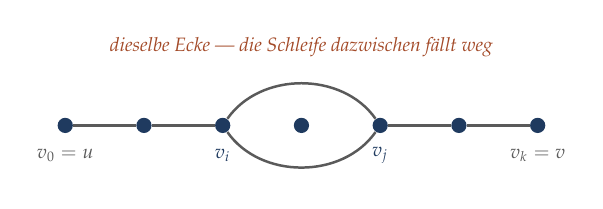
\begin{tikzpicture}[scale=1.0]
\foreach \i/\x in {0/0, 1/1.0, 2/2.0, 3/3.0, 4/4.0, 5/5.0, 6/6.0}
  \node[knoten] (w\i) at (\x,0) {};
\foreach \i/\j in {0/1,1/2,4/5,5/6} \draw[kante] (w\i) -- (w\j);
\draw[kante] (w2) to[bend left=55] (w4);
\draw[kante] (w2) to[bend right=55] (w4);
\node[font=\scriptsize, color=grau] at (0,-0.38) {$v_0=u$};
\node[font=\scriptsize, color=tief] at (2.0,-0.38) {$v_i$};
\node[font=\scriptsize, color=tief] at (4.0,-0.38) {$v_j$};
\node[font=\scriptsize, color=grau] at (6.0,-0.38) {$v_k=v$};
\node[font=\scriptsize\itshape, color=akzent] at (3.0,1.0) {dieselbe Ecke --- die Schleife dazwischen fällt weg};
\end{tikzpicture}
\end{center}

\schritt{Schritt 4 --- Ist $W'$ ein zulässiger Kantenzug?}
Wir müssen prüfen, dass je zwei aufeinanderfolgende Einträge von $W'$ benachbart sind.

Innerhalb des Anfangsstücks $(v_0, \ldots, v_i)$ und innerhalb des Endstücks $(v_{j+1}, \ldots, v_k)$ ist das klar --- diese Paare kamen schon in $W$ vor.

Die einzige neue Nachbarschaft ist die Nahtstelle $v_i \to v_{j+1}$. Nun ist aber $v_i = v_j$ nach Annahme, und $\{v_j, v_{j+1}\}$ war eine Kante von $W$. Also ist
\[ \{v_i, v_{j+1}\} = \{v_j, v_{j+1}\} \in E . \]
$W'$ ist damit ein Kantenzug von $u$ nach $v$.

\schritt{Schritt 5 --- Der Widerspruch}
Die Länge von $W'$ ist $k - (j - i)$. Wegen $i < j$ ist $j - i \ge 1$, also
\[ \text{Länge}(W') \;\le\; k - 1 \;<\; k . \]
Damit gäbe es einen kürzeren Kantenzug von $u$ nach $v$ als $W$ --- im Widerspruch zur Wahl von $W$ in Schritt~1.

\schritt{Schritt 6 --- Schluss}
Die Annahme aus Schritt~2 ist falsch. Also sind alle Ecken von $W$ verschieden, und $W$ ist ein Weg. $\blacksquare$
\end{merksatz}

\begin{merksatz}
\boxtitel{Die Beweisfigur, die hier zum ersten Mal auftritt}
\begin{center}
\begin{minipage}{0.9\textwidth}
\textbf{\enquote{Wähle ein kleinstes Gegenbeispiel und verkleinere es.}}

Man nimmt ein Objekt mit einer Minimalitätseigenschaft, konstruiert daraus ein kleineres mit derselben Eigenschaft und erhält einen Widerspruch. Diese Figur --- das \Begriff{Extremalprinzip} --- kommt in diesem Band noch in den Kapiteln 4, 7, 11 und 13 vor. Sie ersetzt in vielen Fällen eine vollständige Induktion und ist meist kürzer.
\end{minipage}
\end{center}
\end{merksatz}

\section{Zusammenhang und Komponenten}

\begin{definition}
\boxtitelm{Definition 2.4 --- Zusammenhang}
Ein Graph $G$ heißt \Begriff{zusammenhängend}, wenn es zu je zwei Ecken $u, v \in V$ einen Weg von $u$ nach $v$ gibt. Andernfalls heißt $G$ \Begriff{unzusammenhängend}.
\end{definition}

Für die Zerlegung in Gruppen --- Frage (c) --- brauchen wir etwas mehr. Wir definieren eine Beziehung auf der Eckenmenge und zeigen, dass sie die Eckenmenge sauber zerlegt.

\begin{definition}
\boxtitelm{Definition 2.5 --- die Beziehung \enquote{erreichbar}}
Für $u, v \in V$ schreiben wir
\[ u \sim v \quad :\Longleftrightarrow \quad \text{es gibt einen Weg von } u \text{ nach } v \text{ in } G . \]
\end{definition}

\begin{merksatz}
\boxtitel{Satz 2.6 --- $\sim$ ist eine Äquivalenzrelation}
Die Beziehung $\sim$ ist reflexiv, symmetrisch und transitiv.
\end{merksatz}

\begin{merksatz}
\boxtitel{Beweis, alle drei Eigenschaften einzeln}
\schritt{Reflexivität: $u \sim u$ für jede Ecke $u$}
Die Folge $(u)$ ist ein Kantenzug der Länge $0$ von $u$ nach $u$ (Definition 2.1 lässt $k=0$ ausdrücklich zu). Sie besteht aus einer einzigen Ecke, also sind trivialerweise alle Ecken darin verschieden --- es ist ein Weg. Somit $u \sim u$.

\begin{center}
\begin{minipage}{0.88\textwidth}
\kursiv{Hier zahlt sich aus, dass die Definition den Fall $k=0$ zugelassen hat. Hätte man Kantenzüge erst ab Länge $1$ definiert, so wäre eine isolierte Ecke nicht mit sich selbst verbunden --- und der Zusammenhangsbegriff würde absurd.}
\end{minipage}
\end{center}

\schritt{Symmetrie: aus $u \sim v$ folgt $v \sim u$}
Sei $(v_0, v_1, \ldots, v_k)$ ein Weg von $u$ nach $v$. Betrachte die umgekehrte Folge
\[ (v_k, v_{k-1}, \ldots, v_1, v_0) . \]
Sie beginnt bei $v_k = v$ und endet bei $v_0 = u$. Je zwei aufeinanderfolgende Einträge sind benachbart, denn für die Rückwärtsfolge ist das Paar an der Stelle $i$ gerade $\{v_{k-i+1}, v_{k-i}\}$ --- und das ist als Menge dieselbe Kante wie $\{v_{k-i}, v_{k-i+1}\}$, die im ursprünglichen Weg vorkam.

Die Ecken sind dieselben wie vorher, also weiterhin paarweise verschieden. Es ist ein Weg von $v$ nach $u$.

\begin{center}
\begin{minipage}{0.88\textwidth}
\kursiv{An genau dieser Stelle wird gebraucht, dass Kanten \kursiv{Mengen} sind. Bei gerichteten Graphen gilt die Symmetrie nicht --- und dort ist Zusammenhang deshalb ein deutlich komplizierterer Begriff.}
\end{minipage}
\end{center}

\schritt{Transitivität: aus $u \sim v$ und $v \sim w$ folgt $u \sim w$}
Sei $(u = a_0, \ldots, a_r = v)$ ein Weg von $u$ nach $v$ und $(v = b_0, \ldots, b_s = w)$ ein Weg von $v$ nach $w$. Wir hängen sie aneinander:
\[ (a_0, a_1, \ldots, a_{r-1},\ v,\ b_1, b_2, \ldots, b_s) . \]
Das ist ein Kantenzug von $u$ nach $w$: Alle Nachbarschaften stammen aus einem der beiden Wege, und an der Nahtstelle stimmt es, weil $a_r = v = b_0$ ist.

Ein \kursiv{Weg} ist das im Allgemeinen nicht --- die beiden Wege können sich mehrfach kreuzen, und dann käme eine Ecke doppelt vor. Aber nach Lemma 2.3 gibt es dann trotzdem einen Weg von $u$ nach $w$. Also $u \sim w$. $\blacksquare$

\begin{center}
\begin{minipage}{0.88\textwidth}
\kursiv{Das ist der angekündigte Nutzen von Lemma 2.3: Man darf sorglos aneinanderhängen und muss sich nicht darum kümmern, ob dabei Ecken doppelt auftreten.}
\end{minipage}
\end{center}
\end{merksatz}

\begin{merksatz}
\boxtitel{Was eine Äquivalenzrelation liefert --- kurz wiederholt}
Aus Band 10, Kapitel~3 ist bekannt: Eine Äquivalenzrelation auf einer Menge $V$ zerlegt $V$ in \Begriff{Klassen} so, dass
\begin{itemize}[leftmargin=1.4em, itemsep=2pt]
\item jede Ecke in genau einer Klasse liegt,
\item zwei Ecken genau dann in derselben Klasse liegen, wenn sie in Beziehung stehen.
\end{itemize}
Man nennt so etwas eine \Begriff{Partition}: keine Klasse ist leer, die Klassen überschneiden sich nicht, und zusammen ergeben sie ganz $V$.
\end{merksatz}

\begin{definition}
\boxtitelm{Definition 2.7 --- Zusammenhangskomponente}
Die Äquivalenzklassen von $\sim$ heißen \Begriff{Zusammenhangskomponenten} von $G$. Genauer versteht man unter einer Komponente den von einer solchen Klasse $S$ induzierten Teilgraphen $G[S]$.
\end{definition}

\begin{merksatz}
\boxtitel{Die Antwort auf Frage (c)}
\begin{center}
\begin{minipage}{0.9\textwidth}
Satz 2.6 beantwortet die Frage des Hygieneteams vollständig und, wie sich zeigt, mit einer stärkeren Aussage als erhofft: Die Station zerfällt \kursiv{immer} in Gruppen ohne Kontakt untereinander --- die Frage ist nur, in wie viele. Bei einer Gruppe ist der Graph zusammenhängend und alle sind betroffen; bei mehreren ist jede Gruppe für sich zu betrachten.
\end{minipage}
\end{center}

\begin{center}
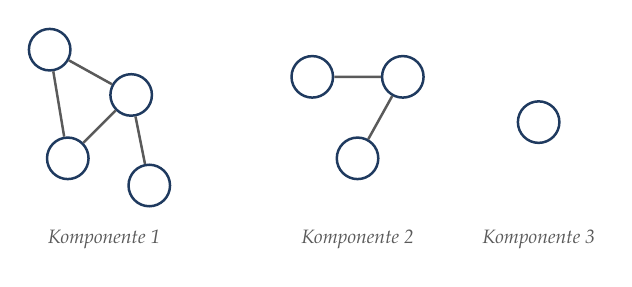
\begin{tikzpicture}[scale=1.15]
\node[knotenb] (a) at (0,0.7) {};
\node[knotenb] (b) at (0.9,0.2) {};
\node[knotenb] (c) at (0.2,-0.5) {};
\node[knotenb] (d) at (1.1,-0.8) {};
\draw[kante] (a)--(b); \draw[kante] (b)--(c); \draw[kante] (c)--(a); \draw[kante] (b)--(d);
\node[knotenb] (e) at (2.9,0.4) {};
\node[knotenb] (f) at (3.9,0.4) {};
\node[knotenb] (g) at (3.4,-0.5) {};
\draw[kante] (e)--(f); \draw[kante] (f)--(g);
\node[knotenb] (h) at (5.4,-0.1) {};
\node[font=\scriptsize\itshape, color=grau] at (0.6,-1.4) {Komponente 1};
\node[font=\scriptsize\itshape, color=grau] at (3.4,-1.4) {Komponente 2};
\node[font=\scriptsize\itshape, color=grau] at (5.4,-1.4) {Komponente 3};
\end{tikzpicture}
\end{center}

Ein Graph ist genau dann zusammenhängend, wenn er \kursiv{genau eine} Komponente hat. Die einzelne Ecke rechts bildet eine eigene Komponente --- sie ist nur mit sich selbst verbunden, und zwar über den Weg der Länge $0$.
\end{merksatz}

\subsection*{Wie viele Kanten braucht Zusammenhang mindestens?}

\begin{merksatz}
\boxtitel{Satz 2.8}
Ein zusammenhängender Graph mit $n$ Ecken hat mindestens $n-1$ Kanten.
\end{merksatz}

\begin{merksatz}
\boxtitel{Beweis durch vollständige Induktion über $n$}
\schritt{Vorbemerkung --- was vollständige Induktion ist}
Um eine Aussage $A(n)$ für alle natürlichen Zahlen $n \ge n_0$ zu zeigen, genügt es:
\begin{itemize}[leftmargin=1.4em, itemsep=2pt]
\item \Begriff{Induktionsanfang}: $A(n_0)$ ist wahr.
\item \Begriff{Induktionsschritt}: Aus der Annahme, dass $A(k)$ für alle $k < n$ gilt, folgt $A(n)$.
\end{itemize}
Der Gedanke: $A(n_0)$ steht fest; damit folgt $A(n_0+1)$; damit $A(n_0+2)$; und so weiter --- jede einzelne Zahl wird nach endlich vielen Schritten erreicht.

\schritt{Induktionsanfang: $n = 1$}
Ein Graph mit einer Ecke ist zusammenhängend (der Weg der Länge $0$ verbindet die Ecke mit sich selbst) und hat $0$ Kanten. Behauptet werden $n - 1 = 0$ Kanten. Erfüllt.

\schritt{Induktionsschritt --- die Vorbereitung}
Sei $n \ge 2$ und $G$ zusammenhängend mit $n$ Ecken. Wir nehmen an, die Behauptung gelte für alle zusammenhängenden Graphen mit weniger als $n$ Ecken.

Zunächst eine Feststellung: In $G$ hat jede Ecke mindestens Grad $1$. Denn wäre $\deg(v) = 0$, so gäbe es von $v$ zu einer anderen Ecke $w$ (die wegen $n \ge 2$ existiert) keinen Weg --- jeder Weg müsste im ersten Schritt eine Kante an $v$ benutzen, und es gibt keine.

\schritt{Fall 1 --- es gibt eine Ecke $v$ mit $\deg(v) = 1$}
Wir entfernen $v$ samt seiner einen Kante und nennen den Rest $G' = G - v$. Er hat $n-1$ Ecken und $|E| - 1$ Kanten.

\kursiv{$G'$ ist zusammenhängend:} Seien $x, y$ zwei Ecken von $G'$. In $G$ gibt es einen Weg von $x$ nach $y$. Könnte dieser Weg über $v$ laufen? Dann käme $v$ als Zwischenecke vor, hätte im Weg also einen Vorgänger \kursiv{und} einen Nachfolger --- das sind zwei verschiedene Nachbarn, im Widerspruch zu $\deg(v) = 1$. Also meidet der Weg die Ecke $v$ und verläuft ganz in $G'$.

Nach Induktionsannahme hat $G'$ mindestens $(n-1) - 1 = n-2$ Kanten. Also
\[ |E| = |E(G')| + 1 \;\ge\; (n-2) + 1 \;=\; n-1 . \]

\schritt{Fall 2 --- jede Ecke hat Grad $\ge 2$}
Dann liefert das Handschlaglemma (Satz 1.3) unmittelbar
\[ 2|E| = \sum_{v \in V} \deg(v) \;\ge\; \sum_{v \in V} 2 \;=\; 2n, \]
also $|E| \ge n \ge n-1$.

\schritt{Schluss}
In beiden Fällen gilt $|E| \ge n-1$. Die beiden Fälle decken alles ab, denn der Minimalgrad ist entweder $1$ (Fall 1, da er nach der Vorbereitung mindestens $1$ ist) oder mindestens $2$ (Fall 2). $\blacksquare$
\end{merksatz}

\begin{merksatz}
\boxtitel{Die Schranke ist scharf}
\enquote{Scharf} heißt: Sie kann nicht verbessert werden, weil es Graphen gibt, die sie mit Gleichheit erfüllen.

Der Weg $P_n$ ist zusammenhängend, hat $n$ Ecken und genau $n-1$ Kanten. Also ist $n-1$ die bestmögliche untere Schranke.

\begin{center}
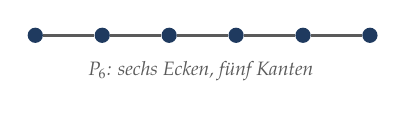
\begin{tikzpicture}[scale=1.0]
\foreach \i in {0,...,5} \node[knoten] (p\i) at (\i*0.85,0) {};
\foreach \i/\j in {0/1,1/2,2/3,3/4,4/5} \draw[kante] (p\i) -- (p\j);
\node[font=\scriptsize\itshape, color=grau] at (2.1,-0.45) {$P_6$: sechs Ecken, fünf Kanten};
\end{tikzpicture}
\end{center}

\begin{center}
\begin{minipage}{0.88\textwidth}
\kursiv{Zu jeder Schranke gehört die Frage, ob sie scharf ist. Eine Schranke ohne dieses Beiwerk sagt wenig: \enquote{mindestens $0$ Kanten} wäre auch wahr und völlig nutzlos. Graphen mit genau $n-1$ Kanten sind der Gegenstand von Kapitel~4.}
\end{minipage}
\end{center}
\end{merksatz}

\section{Abstand}

\begin{definition}
\boxtitelm{Definition 2.9 --- Abstand, Durchmesser, Taille}
Sei $G$ ein Graph und $u,v \in V$.
\begin{itemize}[leftmargin=1.4em, itemsep=4pt]
\item Der \Begriff{Abstand} $d(u,v)$ ist die Länge eines kürzesten Weges von $u$ nach $v$. Gibt es keinen, setzt man $d(u,v) = \infty$.
\item Der \Begriff{Durchmesser} ist $\operatorname{diam}(G) = \max_{u,v \in V} d(u,v)$.
\item Die \Begriff{Taille} $g(G)$ ist die Länge eines kürzesten Kreises in $G$; ist $G$ kreisfrei, setzt man $g(G) = \infty$.
\end{itemize}
\end{definition}

\begin{merksatz}
\boxtitel{Satz 2.10 --- der Abstand ist eine Metrik}
Für alle $u,v,w$ in einer Zusammenhangskomponente gilt:
\begin{center}
\renewcommand{\arraystretch}{1.5}
\begin{tabular}{@{}P{1.2cm}P{3.4cm}P{3.8cm}@{}}
\toprule
(M1) & $d(u,v) \ge 0$, und $d(u,v) = 0 \iff u = v$ & Definitheit\\
(M2) & $d(u,v) = d(v,u)$ & Symmetrie\\
(M3) & $d(u,w) \le d(u,v) + d(v,w)$ & Dreiecksungleichung\\
\bottomrule
\end{tabular}
\end{center}
\end{merksatz}

\begin{merksatz}
\boxtitel{Beweis}
\schritt{(M1)}
Längen sind Anzahlen von Schritten, also $\ge 0$. Ist $u = v$, so ist $(u)$ ein Weg der Länge $0$, also $d(u,v) = 0$. Ist umgekehrt $d(u,v) = 0$, so gibt es einen Weg der Länge $0$; ein solcher besteht aus einem einzigen Eintrag, der zugleich Anfang und Ende ist --- also $u = v$.

\schritt{(M2)}
Im Beweis von Satz 2.6 (Symmetrie) wurde gezeigt: Zu jedem Weg von $u$ nach $v$ der Länge $k$ gibt es einen Weg von $v$ nach $u$ derselben Länge $k$ --- nämlich den umgekehrten. Also haben die Mengen der vorkommenden Weglängen in beiden Richtungen dieselben Elemente und damit dasselbe Minimum.

\schritt{(M3) --- Schritt 1: die beiden kürzesten Wege}
Sei $P$ ein kürzester Weg von $u$ nach $v$ der Länge $a = d(u,v)$ und $Q$ ein kürzester Weg von $v$ nach $w$ der Länge $b = d(v,w)$.

\schritt{(M3) --- Schritt 2: aneinanderhängen}
Wie im Transitivitätsbeweis liefert das Aneinanderhängen einen Kantenzug von $u$ nach $w$ der Länge $a + b$.

\schritt{(M3) --- Schritt 3: der entscheidende Schluss}
Nach Lemma 2.3 gibt es dann einen \kursiv{Weg} von $u$ nach $w$, und aus dem Beweis von Lemma 2.3 sieht man mehr: Der dort konstruierte Weg entsteht durch Weglassen von Stücken, ist also \kursiv{höchstens so lang} wie der Kantenzug. Es gibt somit einen Weg von $u$ nach $w$ der Länge $\le a+b$.

Der kürzeste Weg von $u$ nach $w$ ist erst recht höchstens so lang:
\[ d(u,w) \;\le\; a + b \;=\; d(u,v) + d(v,w) . \qquad \blacksquare \]
\end{merksatz}

\begin{warnung}
\boxtitelr{Warum die Gleichheit in (M3) oft nicht gilt}
Die Dreiecksungleichung ist eine \kursiv{Un}gleichung. Der Umweg über $v$ kann echt länger sein als der direkte Weg.

\begin{center}
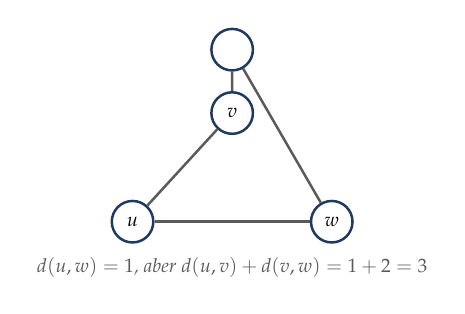
\begin{tikzpicture}[scale=1.15]
\node[knotenb] (u) at (0,0) {$u$};
\node[knotenb] (w) at (2.2,0) {$w$};
\node[knotenb] (v) at (1.1,1.2) {$v$};
\node[knotenb] (x) at (1.1,1.9) {};
\draw[kante] (u) -- (w);
\draw[kante] (u) -- (v); \draw[kante] (v) -- (x); \draw[kante] (x) -- (w);
\node[font=\scriptsize\itshape, color=grau] at (1.1,-0.5) {$d(u,w) = 1$, aber $d(u,v) + d(v,w) = 1 + 2 = 3$};
\end{tikzpicture}
\end{center}
\end{warnung}

\section{Bipartite Graphen}

\begin{definition}
\boxtitelm{Definition 2.11 --- bipartit}
Ein Graph $G = (V,E)$ heißt \Begriff{bipartit}, wenn sich $V$ so in zwei Mengen $A$ und $B$ zerlegen lässt, dass
\[ V = A \cup B, \qquad A \cap B = \varnothing, \]
und \kursiv{jede} Kante von $G$ eine Ecke aus $A$ mit einer Ecke aus $B$ verbindet. Das Paar $(A,B)$ heißt eine \Begriff{Bipartition}.
\end{definition}

In der Sprache des Dienstplans: Bipartit heißt, dass zwei Schichten genügen. Das führt auf die zweite Frage aus Kapitel~1 zurück und ist zugleich der einfachste Fall des Färbungsproblems aus Kapitel~9.

Wie erkennt man Bipartitheit? Der folgende Satz gibt ein Kriterium, das man auch bei großen Graphen prüfen kann.

\begin{merksatz}
\boxtitel{Satz 2.12 (Kőnig 1916)}
Ein Graph ist genau dann bipartit, wenn er keinen Kreis ungerader Länge enthält.
\end{merksatz}

\begin{merksatz}
\boxtitel{Beweis, Richtung 1: bipartit $\Longrightarrow$ kein ungerader Kreis}
\schritt{Schritt 1 --- Aufstellung}
Sei $(A,B)$ eine Bipartition und sei $(v_0, v_1, \ldots, v_k)$ mit $v_k = v_0$ ein Kreis in $G$.

\schritt{Schritt 2 --- die Seiten wechseln sich ab}
Jede Kante verbindet eine Ecke aus $A$ mit einer aus $B$. Da $\{v_{i-1},v_i\}$ für jedes $i$ eine Kante ist, liegen $v_{i-1}$ und $v_i$ stets auf \kursiv{verschiedenen} Seiten. Mit jedem Schritt wechselt man also die Seite.

\schritt{Schritt 3 --- die Buchführung}
Nehmen wir ohne Einschränkung $v_0 \in A$ an (sonst vertauscht man die Rollen von $A$ und $B$). Dann gilt:
\begin{center}
\renewcommand{\arraystretch}{1.4}
\begin{tabular}{@{}P{2.4cm}P{2.4cm}@{}}
\toprule
$v_0 \in A$ & $0$ ist gerade\\
$v_1 \in B$ & $1$ ist ungerade\\
$v_2 \in A$ & $2$ ist gerade\\
\multicolumn{2}{@{}l}{\quad allgemein: $v_i \in A \iff i$ gerade}\\
\bottomrule
\end{tabular}
\end{center}

\schritt{Schritt 4 --- Schluss}
Am Ende ist $v_k = v_0 \in A$. Nach der Regel aus Schritt~3 muss dann $k$ gerade sein. Ein ungerader Kreis kann also nicht vorkommen.
\end{merksatz}

\begin{merksatz}
\boxtitel{Beweis, Richtung 2: kein ungerader Kreis $\Longrightarrow$ bipartit}
\schritt{Schritt 1 --- Reduktion auf den zusammenhängenden Fall}
Wenn jede Komponente für sich bipartit ist, so ist es der ganze Graph: Man vereinigt einfach die $A$-Seiten aller Komponenten zu einem $A$ und die $B$-Seiten zu einem $B$. Da zwischen Komponenten keine Kanten verlaufen, entsteht kein Konflikt. Wir dürfen also $G$ als zusammenhängend annehmen.

\schritt{Schritt 2 --- die Konstruktion}
Wir wählen eine feste Ecke $r \in V$ (die \Begriff{Wurzel}) und setzen
\[ A = \{\, v \in V : d(r,v) \text{ ist gerade} \,\}, \qquad
   B = \{\, v \in V : d(r,v) \text{ ist ungerade} \,\} . \]
Da $G$ zusammenhängend ist, ist $d(r,v)$ für jede Ecke eine endliche Zahl. Jede Ecke landet in genau einer der beiden Mengen, denn jede natürliche Zahl ist entweder gerade oder ungerade. Also ist $V = A \cup B$ und $A \cap B = \varnothing$. Beachte $r \in A$ wegen $d(r,r) = 0$.

\schritt{Schritt 3 --- was noch zu zeigen ist}
Es bleibt: \kursiv{Keine Kante verläuft innerhalb von $A$ oder innerhalb von $B$.} Angenommen doch --- es gäbe eine Kante $\{x,y\} \in E$ mit $x, y$ auf derselben Seite. Das heißt: $d(r,x)$ und $d(r,y)$ sind beide gerade oder beide ungerade. In jedem Fall ist die Differenz gerade:
\[ d(r,x) - d(r,y) \ \text{ist eine gerade Zahl.} \]

\schritt{Schritt 4 --- zwei kürzeste Wege betrachten}
Sei $P$ ein kürzester Weg von $r$ nach $x$ (Länge $p = d(r,x)$) und $Q$ ein kürzester Weg von $r$ nach $y$ (Länge $q = d(r,y)$).

Die beiden Wege beginnen beide bei $r$. Sie können sich ein Stück weit decken und trennen sich dann. Sei $z$ die \kursiv{letzte} Ecke, die auf beiden Wegen vorkommt --- sie existiert, weil zumindest $r$ auf beiden liegt, und es gibt nur endlich viele Kandidaten.

\begin{center}
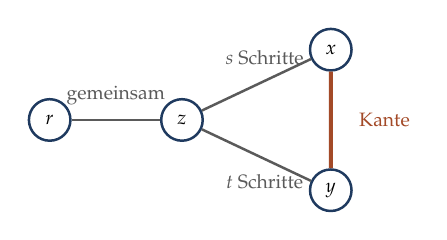
\begin{tikzpicture}[scale=1.05]
\node[knotenb] (r) at (0,0) {$r$};
\node[knotenb] (z) at (1.6,0) {$z$};
\node[knotenb] (x) at (3.4,0.85) {$x$};
\node[knotenb] (y) at (3.4,-0.85) {$y$};
\draw[kante] (r) -- (z);
\draw[kante] (z) -- (x);
\draw[kante] (z) -- (y);
\draw[kanted] (x) -- (y);
\node[font=\scriptsize, color=grau] at (0.8,0.3) {gemeinsam};
\node[font=\scriptsize, color=grau] at (2.6,0.75) {$s$ Schritte};
\node[font=\scriptsize, color=grau] at (2.6,-0.75) {$t$ Schritte};
\node[font=\scriptsize, color=akzent] at (4.05,0) {Kante};
\end{tikzpicture}
\end{center}

\schritt{Schritt 5 --- die Längen}
Ein Teilstück eines kürzesten Weges ist selbst ein kürzester Weg. Denn gäbe es zwischen zwei seiner Ecken eine kürzere Verbindung, so könnte man sie einsetzen und den Gesamtweg verkürzen --- im Widerspruch zur Kürze. Also ist der Abschnitt von $r$ nach $z$ auf $P$ ein kürzester Weg, und dasselbe gilt auf $Q$. Beide Abschnitte haben daher dieselbe Länge, nämlich $d(r,z)$; nennen wir sie $c$.

Damit hat der Abschnitt von $z$ nach $x$ die Länge $s = p - c$ und der von $z$ nach $y$ die Länge $t = q - c$.

\schritt{Schritt 6 --- der Kreis}
Wir setzen zusammen: von $z$ nach $x$ ($s$ Schritte), die Kante $\{x,y\}$ ($1$ Schritt), von $y$ zurück nach $z$ ($t$ Schritte). Das ergibt einen geschlossenen Kantenzug der Länge
\[ s + 1 + t = (p - c) + 1 + (q - c) = p + q + 1 - 2c . \]

Dieser geschlossene Kantenzug ist sogar ein Kreis: Die Ecken der beiden Abschnitte sind jeweils untereinander verschieden (Teilstücke von Wegen), und sie haben nach Wahl von $z$ außer $z$ selbst keine gemeinsame Ecke.

\schritt{Schritt 7 --- die Parität}
Nach Schritt~3 ist $p - q$ gerade, also haben $p$ und $q$ dieselbe Parität, also ist $p+q$ gerade. Ferner ist $2c$ gerade. Somit ist
\[ s + 1 + t = \underbrace{p+q}_{\text{gerade}} + 1 - \underbrace{2c}_{\text{gerade}} \quad \text{ungerade.} \]

Wir haben einen Kreis ungerader Länge gefunden --- im Widerspruch zur Voraussetzung.

\schritt{Schritt 8 --- Schluss}
Die Annahme aus Schritt~3 war falsch. Jede Kante verläuft also zwischen $A$ und $B$, und $(A,B)$ ist eine Bipartition. $\blacksquare$
\end{merksatz}

\begin{merksatz}
\boxtitel{Wie man das praktisch anwendet}
Der Beweis von Richtung 2 ist nicht nur ein Beweis, sondern ein \kursiv{Verfahren}: Man wählt eine Wurzel, berechnet alle Abstände, färbt nach gerade/ungerade und prüft zum Schluss jede Kante. Findet man eine Kante innerhalb einer Seite, liefert Schritt~6 sogar den ungeraden Kreis, der die Bipartitheit verhindert --- man bekommt also nicht nur ein Nein, sondern die Begründung dazu.

\begin{center}
\begin{minipage}{0.88\textwidth}
\kursiv{Beweise, die zugleich Verfahren sind, heißen \Begriff{konstruktiv}. Sie sind in der Graphentheorie die Regel und der Grund, warum das Gebiet und die Informatik so eng beieinander liegen.}
\end{minipage}
\end{center}
\end{merksatz}

\section{Brücken und Schnittecken}

Bleibt Frage (d): Gibt es eine einzelne Person, deren Isolierung die Station teilt?

\begin{definition}
\boxtitelm{Definition 2.13 --- Brücke, Schnittecke}
Sei $G$ ein Graph.
\begin{itemize}[leftmargin=1.4em, itemsep=4pt]
\item Eine Kante $e \in E$ heißt \Begriff{Brücke}, wenn $G - e$ mehr Komponenten hat als $G$.
\item Eine Ecke $v \in V$ heißt \Begriff{Schnittecke}, wenn $G - v$ mehr Komponenten hat als $G$.
\end{itemize}
Dabei entsteht $G-e$ durch Weglassen der Kante $e$, und $G-v$ durch Weglassen der Ecke $v$ \kursiv{samt aller Kanten}, die $v$ berühren.
\end{definition}

\begin{merksatz}
\boxtitel{Satz 2.14}
Eine Kante $e$ ist genau dann eine Brücke, wenn sie auf keinem Kreis von $G$ liegt.
\end{merksatz}

\begin{merksatz}
\boxtitel{Beweis}
Sei $e = \{x,y\}$.

\schritt{Richtung 1 --- liegt $e$ auf einem Kreis, so ist $e$ keine Brücke}
Sei $C = (x, y, w_1, w_2, \ldots, w_r, x)$ ein Kreis durch $e$. Dann ist
\[ R = (x, w_r, w_{r-1}, \ldots, w_1, y) \]
ein Weg von $x$ nach $y$, der die Kante $e$ nicht benutzt --- er läuft ja auf der anderen Seite des Kreises herum.

Nun sei $u,v$ ein beliebiges Eckenpaar, das in $G$ durch einen Weg verbunden ist. Benutzt dieser Weg die Kante $e$ nicht, so besteht er auch in $G - e$. Benutzt er sie, so ersetzen wir das Kantenstück $x \to y$ durch den Umweg $R$ und erhalten einen Kantenzug in $G-e$; nach Lemma 2.3 gibt es dann auch dort einen Weg. In beiden Fällen bleibt $u \sim v$ erhalten. Die Komponentenzahl ändert sich also nicht.

\schritt{Richtung 2 --- ist $e$ keine Brücke, so liegt $e$ auf einem Kreis}
Ist $e$ keine Brücke, so hat $G-e$ dieselbe Komponentenzahl wie $G$. Insbesondere liegen $x$ und $y$ auch in $G-e$ in derselben Komponente --- denn in $G$ tun sie es (die Kante $e$ verbindet sie), und die Komponenten können durch Entfernen einer Kante nur zerfallen, nicht verschmelzen; bliebe $x$ von $y$ getrennt, wären es mehr Komponenten.

Es gibt also einen Weg $P$ von $x$ nach $y$ in $G - e$. Seine Länge ist mindestens $2$, denn die einzige Kante der Länge $1$ zwischen $x$ und $y$ wäre $e$, und die fehlt.

Hängen wir an $P$ die Kante $e$ an, so entsteht ein geschlossener Kantenzug der Länge $\ge 3$, in dem alle Ecken bis auf Anfang und Ende verschieden sind --- also ein Kreis durch $e$. $\blacksquare$
\end{merksatz}

\begin{warnung}
\boxtitelr{Kein entsprechender Satz für Schnittecken}
Es liegt nahe zu vermuten: \enquote{Eine Ecke ist genau dann Schnittecke, wenn sie auf keinem Kreis liegt.} Das ist falsch.

\begin{center}
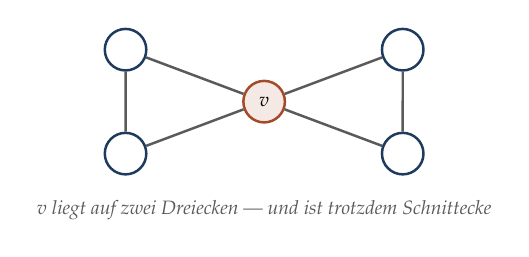
\begin{tikzpicture}[scale=1.1]
\node[knotenb] (a) at (-1.6,0.6) {};
\node[knotenb] (b) at (-1.6,-0.6) {};
\node[knotenr] (v) at (0,0) {$v$};
\node[knotenb] (c) at (1.6,0.6) {};
\node[knotenb] (d) at (1.6,-0.6) {};
\draw[kante] (a)--(b); \draw[kante] (a)--(v); \draw[kante] (b)--(v);
\draw[kante] (c)--(d); \draw[kante] (c)--(v); \draw[kante] (d)--(v);
\node[font=\scriptsize\itshape, color=grau] at (0,-1.25) {$v$ liegt auf zwei Dreiecken --- und ist trotzdem Schnittecke};
\end{tikzpicture}
\end{center}

Entfernt man $v$, zerfällt der Graph in zwei Dreieckshälften. Die Ecke liegt auf Kreisen, ist aber der einzige Übergang zwischen den beiden Teilen.

\begin{center}
\begin{minipage}{0.88\textwidth}
\kursiv{Das ist ein gutes Beispiel dafür, wie unzuverlässig Analogieschlüsse in der Graphentheorie sind. Der richtige Begriff für \enquote{es gibt keine Schnittecke} heißt \Begriff{zweifach zusammenhängend} und wird in Kapitel~12 im Zusammenhang mit dem Satz von Menger behandelt.}
\end{minipage}
\end{center}
\end{warnung}

\section{Übungsaufgaben}

\begin{aufgabe}
\boxtitel{Aufgabe 2.1 --- Komponenten und Kantenzahl}
Ein Graph hat $10$ Ecken und $3$ Zusammenhangskomponenten. Wie viele Kanten hat er mindestens?

\loesung
\schritt{Schritt 1 --- Die Komponenten einzeln betrachten}
Seien die Komponenten $n_1$, $n_2$, $n_3$ Ecken groß mit $n_1 + n_2 + n_3 = 10$ und $n_i \ge 1$.

Jede Komponente ist für sich ein zusammenhängender Graph. Nach Satz 2.8 hat die $i$-te also mindestens $n_i - 1$ Kanten.

\schritt{Schritt 2 --- Aufsummieren}
Da Kanten nie zwischen Komponenten verlaufen, ist die Gesamtkantenzahl die Summe:
\[ |E| \;\ge\; (n_1 - 1) + (n_2 - 1) + (n_3 - 1) = (n_1+n_2+n_3) - 3 = 10 - 3 = 7 . \]

\schritt{Schritt 3 --- Ist die Schranke erreichbar?}
Ja. Man nehme drei Wege, etwa $P_8$, $P_1$, $P_1$: Der erste hat $7$ Kanten, die beiden einzelnen Ecken keine. Zusammen $8+1+1 = 10$ Ecken, $3$ Komponenten, $7$ Kanten.

\schritt{Antwort}
Mindestens $\mathbf{7}$ Kanten. Allgemein gilt: Ein Graph mit $n$ Ecken und $c$ Komponenten hat mindestens $n - c$ Kanten.
\end{aufgabe}

\begin{aufgabe}
\boxtitel{Aufgabe 2.2 --- Abstände im Petersen-Graphen}
Bestimmen Sie Durchmesser und Taille des Petersen-Graphen.

\loesung
\schritt{Schritt 1 --- Aufbau in Erinnerung rufen}
Fünf äußere Ecken $a_0, \ldots, a_4$ bilden einen Fünfeckskreis. Fünf innere Ecken $b_0, \ldots, b_4$ sind so verbunden, dass $b_i$ mit $b_{i+2}$ benachbart ist (Indizes stets modulo $5$ gerechnet). Jede Speiche verbindet $a_i$ mit $b_i$.

\schritt{Schritt 2 --- Die Taille: gibt es ein Dreieck?}
Wir prüfen die drei möglichen Sorten von Dreiecken.
\begin{center}
{\small
\renewcommand{\arraystretch}{1.42}
\begin{tabular}{@{}P{2.6cm}P{5.4cm}@{}}
\toprule
Drei äußere & Der äußere Kreis hat Länge $5$; er enthält keine Sehne, denn $a_i$ ist nur mit $a_{i\pm1}$ und $b_i$ benachbart. Kein Dreieck.\\
Drei innere & $b_i$ ist mit $b_{i\pm 2}$ benachbart. Wären $b_i, b_j, b_k$ ein Dreieck, so müssten die drei Differenzen alle $\pm 2$ sein --- aber $2+2+2 = 6 \not\equiv 0$ und $2+2-2 = 2 \not\equiv 0$ modulo $5$. Kein Dreieck.\\
Gemischt & Jede Ecke hat genau eine Speiche. Ein Dreieck mit zwei äußeren und einer inneren Ecke bräuchte zwei Speichen zu derselben inneren Ecke --- gibt es nicht. Ebenso umgekehrt.\\
\bottomrule
\end{tabular}}
\end{center}

\schritt{Schritt 3 --- Gibt es einen Vierkreis?}
Ein Vierkreis müsste eine gerade Anzahl von Speichen benutzen, also $0$, $2$ oder $4$.

\kursiv{Null Speichen:} ganz außen (der äußere Kreis hat Länge $5$, ohne Sehnen --- unmöglich) oder ganz innen (der innere Fünfstern hat ebenfalls Länge $5$ als Kreis, ohne kürzere --- unmöglich).

\kursiv{Zwei Speichen:} Der Kreis hätte die Form $a_i \to a_j \to b_j \to b_i \to a_i$. Dann müsste $a_i a_j$ eine Kante sein, also $j = i \pm 1$, \kursiv{und} $b_i b_j$ eine Kante, also $j = i \pm 2$. Beides zugleich ist unmöglich.

\kursiv{Vier Speichen:} Dann wechselten sich vier Speichen ab, ohne dazwischen andere Kanten --- der Kreis hätte Länge $8$, nicht $4$.

\schritt{Schritt 4 --- Ein Fünfkreis existiert}
Der äußere Kreis $a_0 a_1 a_2 a_3 a_4 a_0$ hat Länge $5$. Also
\[ g(\text{Petersen}) = \mathbf{5} . \]

\schritt{Schritt 5 --- Der Durchmesser}
Wir bestimmen die Abstände von $a_0$ aus.
\begin{center}
\renewcommand{\arraystretch}{1.42}
\begin{tabular}{@{}P{1.8cm}P{4.2cm}P{1.4cm}@{}}
\toprule
\textbf{Abstand} & \textbf{Ecken} & \textbf{Anzahl}\\
\midrule
$0$ & $a_0$ & $1$\\
$1$ & $a_1$, $a_4$, $b_0$ & $3$\\
$2$ & $a_2$, $a_3$, $b_1$, $b_4$, $b_2$, $b_3$ & $6$\\
\bottomrule
\end{tabular}
\end{center}
Zur Kontrolle der dritten Zeile: $a_2$ über $a_1$; $a_3$ über $a_4$; $b_1$ über $a_1$; $b_4$ über $a_4$; $b_2$ über $b_0$ (denn $b_0 b_2$ ist eine Kante); $b_3$ über $b_0$ (denn $b_0 b_3 = b_0 b_{0-2}$ ist eine Kante).

$1 + 3 + 6 = 10$ --- alle Ecken erfasst. Der größte Abstand von $a_0$ aus ist $2$.

\schritt{Schritt 6 --- Warum das für alle Ecken gilt}
Der Petersen-Graph ist \Begriff{eckentransitiv}: Zu je zwei Ecken gibt es einen Isomorphismus des Graphen auf sich selbst, der die eine in die andere überführt. Deshalb sieht der Graph von jeder Ecke aus gleich aus, und die Rechnung von $a_0$ aus gilt überall.
\[ \operatorname{diam}(\text{Petersen}) = \mathbf{2} . \]

\schritt{Probe}
Bei Grad $3$ und Durchmesser $2$ erreicht man von einer Ecke aus höchstens $1 + 3 + 3\cdot 2 = 10$ Ecken. Der Petersen-Graph erreicht genau $10$ --- er ist ein sogenannter Moore-Graph, der diese Schranke mit Gleichheit erfüllt. Das erklärt seinen Sonderstatus. \checkmark
\end{aufgabe}

\begin{aufgabe}
\boxtitel{Aufgabe 2.3 --- Bipartit oder nicht?}
Ist der abgebildete Graph bipartit? Geben Sie eine Bipartition an oder einen ungeraden Kreis.

\begin{center}
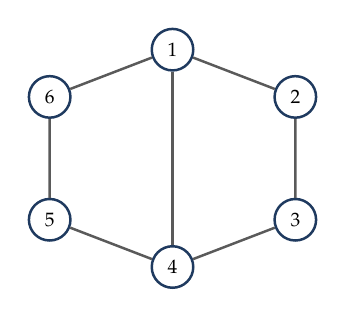
\begin{tikzpicture}[scale=1.2]
\node[knotenb] (1) at (0,1.1) {$1$};
\node[knotenb] (2) at (1.3,0.6) {$2$};
\node[knotenb] (3) at (1.3,-0.7) {$3$};
\node[knotenb] (4) at (0,-1.2) {$4$};
\node[knotenb] (5) at (-1.3,-0.7) {$5$};
\node[knotenb] (6) at (-1.3,0.6) {$6$};
\draw[kante] (1)--(2); \draw[kante] (2)--(3); \draw[kante] (3)--(4);
\draw[kante] (4)--(5); \draw[kante] (5)--(6); \draw[kante] (6)--(1);
\draw[kante] (1)--(4);
\end{tikzpicture}
\end{center}

\loesung
\schritt{Schritt 1 --- Das Verfahren aus dem Beweis anwenden}
Wurzel: $r = 1$. Wir bestimmen die Abstände.

\begin{center}
\renewcommand{\arraystretch}{1.42}
\begin{tabular}{@{}P{1.4cm}P{3.4cm}P{1.4cm}P{1.4cm}@{}}
\toprule
\textbf{Ecke} & \textbf{Kürzester Weg} & $d(1,v)$ & \textbf{Seite}\\
\midrule
$1$ & --- & $0$ & $A$\\
$2$ & $1\!-\!2$ & $1$ & $B$\\
$6$ & $1\!-\!6$ & $1$ & $B$\\
$4$ & $1\!-\!4$ & $1$ & $B$\\
$3$ & $1\!-\!2\!-\!3$ & $2$ & $A$\\
$5$ & $1\!-\!6\!-\!5$ & $2$ & $A$\\
\bottomrule
\end{tabular}
\end{center}

Also $A = \{1, 3, 5\}$ und $B = \{2, 4, 6\}$.

\schritt{Schritt 2 --- Jede Kante prüfen}
\begin{center}
\renewcommand{\arraystretch}{1.4}
\begin{tabular}{@{}P{1.6cm}P{2.6cm}P{2.4cm}@{}}
\toprule
\textbf{Kante} & \textbf{Seiten} & \textbf{In Ordnung?}\\
\midrule
$\{1,2\}$ & $A$--$B$ & ja\\
$\{2,3\}$ & $B$--$A$ & ja\\
$\{3,4\}$ & $A$--$B$ & ja\\
$\{4,5\}$ & $B$--$A$ & ja\\
$\{5,6\}$ & $A$--$B$ & ja\\
$\{6,1\}$ & $B$--$A$ & ja\\
$\{1,4\}$ & $A$--$B$ & ja\\
\bottomrule
\end{tabular}
\end{center}

Alle sieben Kanten verlaufen zwischen den Seiten.

\schritt{Antwort}
Der Graph ist bipartit mit der Bipartition $A = \{1,3,5\}$, $B = \{2,4,6\}$.

\schritt{Gegenprobe über Satz 2.12}
Der Graph enthält die Kreise $1\!-\!2\!-\!3\!-\!4\!-\!1$ (Länge $4$), $1\!-\!4\!-\!5\!-\!6\!-\!1$ (Länge $4$) und den äußeren Sechskreis (Länge $6$). Alle gerade --- passt zum Ergebnis. \checkmark

\schritt{Was passiert, wenn man eine Kante hinzufügt}
Fügt man $\{1,3\}$ hinzu, so entsteht das Dreieck $1\!-\!2\!-\!3\!-\!1$: ein ungerader Kreis. Der Graph wäre dann nicht mehr bipartit, und es bräuchte drei Schichten statt zwei.
\end{aufgabe}

\begin{aufgabe}
\boxtitel{Aufgabe 2.4 --- Ein Satz über den Durchmesser}
Zeigen Sie: Ist $G$ zusammenhängend mit $\operatorname{diam}(G) \ge 3$, so ist das Komplement $\overline{G}$ zusammenhängend mit $\operatorname{diam}(\overline{G}) \le 3$.

\loesung
\schritt{Schritt 1 --- Was zu zeigen ist}
Für je zwei verschiedene Ecken $u,v$ ist ein Weg in $\overline{G}$ der Länge höchstens $3$ anzugeben.

\schritt{Schritt 2 --- Die Voraussetzung ausnutzen}
Wegen $\operatorname{diam}(G) \ge 3$ gibt es Ecken $x, y$ mit $d_G(x,y) \ge 3$.

Daraus folgt zweierlei:
\begin{itemize}[leftmargin=1.4em, itemsep=2pt]
\item $\{x,y\} \notin E$, sonst wäre $d_G(x,y) = 1$;
\item $N_G(x) \cap N_G(y) = \varnothing$, denn ein gemeinsamer Nachbar $z$ ergäbe den Weg $x\!-\!z\!-\!y$ und damit $d_G(x,y) \le 2$.
\end{itemize}
Insbesondere ist in $\overline{G}$ jede Ecke mit $x$ oder mit $y$ benachbart: Eine Ecke $w \notin \{x,y\}$ kann in $G$ nicht zugleich Nachbar von $x$ und von $y$ sein, ist also in $\overline{G}$ Nachbar von mindestens einem der beiden.

\schritt{Schritt 3 --- Fallunterscheidung für zwei Ecken $u,v$}

\textbf{Fall A: $\{u,v\} \notin E$.} Dann ist $\{u,v\}$ eine Kante von $\overline{G}$, also $d_{\overline{G}}(u,v) = 1$.

\textbf{Fall B: $\{u,v\} \in E$.} Dann ist $\{u,v\}$ keine Kante von $\overline{G}$, und wir brauchen einen Umweg.

Nach Schritt~2 ist $u$ in $\overline{G}$ mit $x$ oder $y$ benachbart; dasselbe gilt für $v$.

\kursiv{Fall B1 --- beide mit derselben dieser Ecken, sagen wir $x$.} Falls $u = x$ oder $v = x$, ist einer der beiden schon $x$ und der Weg hat Länge $1$; andernfalls ist $u\!-\!x\!-\!v$ ein Weg in $\overline{G}$ der Länge $2$.

\kursiv{Fall B2 --- $u$ mit $x$, $v$ mit $y$ (oder umgekehrt).} Da $\{x,y\} \notin E$, ist $\{x,y\}$ eine Kante von $\overline{G}$. Also ist
\[ u \;-\; x \;-\; y \;-\; v \]
ein Kantenzug in $\overline{G}$ der Länge $3$. Nach Lemma 2.3 gibt es einen Weg von $u$ nach $v$ der Länge höchstens $3$.

\schritt{Schritt 4 --- Schluss}
In allen Fällen ist $d_{\overline{G}}(u,v) \le 3$. Also ist $\overline{G}$ zusammenhängend, und sein Durchmesser ist höchstens $3$. $\blacksquare$

\schritt{Probe an einem Beispiel}
$G = P_4$ (Weg auf $1,2,3,4$) hat $\operatorname{diam} = 3$. Das Komplement hat die Kanten $\{1,3\}, \{1,4\}, \{2,4\}$ --- das ist wieder ein $P_4$, nämlich $3\!-\!1\!-\!4\!-\!2$, mit Durchmesser $3$. Die Schranke ist also scharf. \checkmark
\end{aufgabe}

\begin{geschichte}
\boxtitelg{Dénes Kőnig und der Satz über bipartite Graphen}
\Person{Dénes Kőnig} (1884--1944) bewies den Satz 2.12 im Jahr 1916, in derselben Arbeit, die auch den nach ihm benannten Satz über Paarungen enthält (Kapitel~11). Er lehrte in Budapest und schrieb 1936 das erste Lehrbuch des Gebiets --- deutschsprachig, im Leipziger Verlag Akademische Verlagsgesellschaft erschienen.

Sein Vater \Person{Gyula Kőnig} war ebenfalls Mathematiker und in der Mengenlehre bekannt geworden. Dénes Kőnig nahm sich 1944 das Leben, wenige Tage nach der deutschen Besetzung Ungarns.

\begin{center}
\begin{minipage}{0.9\textwidth}
\kursiv{Sein Buch ist der Grund, warum ein großer Teil der Grundbegriffe --- \enquote{Ecke}, \enquote{Kante}, \enquote{Grad}, \enquote{Baum} --- deutsche Ursprünge hat. Die englische Terminologie entstand erst nach 1945, teils als Übersetzung, teils als Neuschöpfung.}
\end{minipage}
\end{center}
\end{geschichte}

\begin{forschung}
\boxtitelp{Kleine Durchmesser in großen Netzen}
Der Durchmesser wirklicher Netzwerke ist erstaunlich klein. Das Weltnetz der Verweise hat bei über $10^{11}$ Ecken einen mittleren Abstand von etwa $19$; im Netz der Koautorenschaften in der Mathematik liegt er bei ungefähr $7{,}6$.

Die theoretische Erklärung liefern Zufallsgraphmodelle: Bereits ein Zufallsgraph, in dem jede Ecke im Mittel $c > 1$ Nachbarn hat, hat mit hoher Wahrscheinlichkeit einen Durchmesser der Größenordnung $\log n / \log c$. Wächst $n$ um den Faktor $1000$, wächst der Durchmesser nur um etwa $3$. Kapitel~14 rechnet das nach.

\begin{center}
\begin{minipage}{0.9\textwidth}
\kursiv{Vorsicht ist geboten bei der populären Formulierung \enquote{jeder kennt jeden über sechs Ecken}. Sie geht auf ein Experiment von Stanley Milgram (1967) zurück, das methodisch schwach war: Die Rücklaufquote lag unter einem Drittel, und gescheiterte Ketten wurden nicht gezählt. Die Größenordnung hat sich später bestätigt, das berühmte Ergebnis selbst trug sie nicht.}
\end{minipage}
\end{center}
\end{forschung}

\begin{merksatz}
\boxtitel{Was Sie jetzt können}
\begin{center}
\renewcommand{\arraystretch}{1.5}
\begin{tabular}{@{}P{3.0cm}P{5.6cm}@{}}
\toprule
\textbf{Sprache} & Kantenzug, Weg, Kreis --- und der Unterschied\\
\textbf{Lemma 2.3} & Jeder Kantenzug enthält einen Weg\\
\textbf{Satz 2.6} & Erreichbarkeit ist eine Äquivalenzrelation; daher zerfällt jeder Graph in Komponenten\\
\textbf{Satz 2.8} & Zusammenhang kostet mindestens $n-1$ Kanten\\
\textbf{Satz 2.10} & Der Abstand ist eine Metrik\\
\textbf{Satz 2.12} & Bipartit $\iff$ kein ungerader Kreis --- mit Verfahren\\
\textbf{Satz 2.14} & Brücke $\iff$ auf keinem Kreis\\
\bottomrule
\end{tabular}
\end{center}
\end{merksatz}

\chapter{Wie man Graphen aufschreibt}

\section{Warum Bilder nicht genügen}

Ein Graph mit zwölf Ecken lässt sich zeichnen. Einer mit tausend nicht mehr sinnvoll, und einer mit einer Million schon gar nicht. Spätestens dann braucht man eine Schreibweise, die

\begin{center}
\renewcommand{\arraystretch}{1.5}
\begin{tabular}{@{}P{1.0cm}P{7.4cm}@{}}
\toprule
(a) & eindeutig ist --- zwei Menschen lesen dasselbe heraus,\\
(b) & sich rechnen lässt --- man kann Eigenschaften ausrechnen, statt sie abzulesen,\\
(c) & sparsam ist --- der Platzbedarf soll zum Graphen passen.\\
\bottomrule
\end{tabular}
\end{center}

Es gibt drei gebräuchliche Antworten. Die dritte ist die sparsamste, die erste die rechenfreundlichste --- und die erste liefert überraschenderweise einen Satz, der die Zahl aller Wege einer gegebenen Länge angibt.

\section{Was eine Matrix ist}

Bevor wir die erste Darstellung angeben, klären wir den Begriff. Wer Band 2 der Reihe kennt, kann diesen Abschnitt überspringen.

\begin{definition}
\boxtitelm{Definition 3.1 --- Matrix}
Eine \Begriff{Matrix} mit $n$ Zeilen und $n$ Spalten ist eine rechteckige Anordnung von Zahlen. Man schreibt
\[ A = \begin{pmatrix}
a_{11} & a_{12} & \cdots & a_{1n} \\
a_{21} & a_{22} & \cdots & a_{2n} \\
\vdots & \vdots & \ddots & \vdots \\
a_{n1} & a_{n2} & \cdots & a_{nn}
\end{pmatrix} \]
und bezeichnet mit $a_{ij}$ die Zahl in der $i$-ten Zeile und der $j$-ten Spalte.
\end{definition}

\begin{warnung}
\boxtitelr{Zeile zuerst, Spalte zweitens}
Bei $a_{ij}$ ist $i$ die \kursiv{Zeile} und $j$ die \kursiv{Spalte} --- immer in dieser Reihenfolge. Das Verwechseln dieser beiden Indizes ist die häufigste Fehlerquelle beim Rechnen mit Matrizen.

Eine Eselsbrücke: \enquote{Zeilen zuerst, Spalten später} --- alphabetisch und im Alphabet steht Z vor S nicht; die Merkhilfe funktioniert stattdessen über die Form: Man liest wie einen Text erst \kursiv{nach unten} bis zur richtigen Zeile, dann \kursiv{nach rechts} bis zur richtigen Spalte.
\end{warnung}

\section{Die Adjazenzmatrix}

\begin{definition}
\boxtitelm{Definition 3.2 --- Adjazenzmatrix}
Sei $G$ ein Graph, dessen Ecken in einer festen Reihenfolge $v_1, v_2, \ldots, v_n$ durchnummeriert sind. Die \Begriff{Adjazenzmatrix} $A = A(G)$ ist die $n \times n$-Matrix mit
\[ a_{ij} = \begin{cases} 1, & \text{falls } \{v_i, v_j\} \in E, \\[2pt] 0, & \text{sonst.} \end{cases} \]
\end{definition}

\begin{merksatz}
\boxtitel{Ein Beispiel, vollständig ausgeschrieben}
Wir nehmen den Dienstplangraphen aus Kapitel~1 mit der Nummerierung $v_1 = A$, $v_2 = B$, $v_3 = C$, $v_4 = D$, $v_5 = E$ und den Kanten $AB$, $AC$, $BC$, $BD$, $CE$, $DE$.

\schritt{Feld für Feld}
Wir gehen die erste Zeile durch. Sie gehört zur Ecke $A$.
\begin{center}
{\small
\renewcommand{\arraystretch}{1.4}
\begin{tabular}{@{}P{1.4cm}P{3.6cm}P{1.4cm}@{}}
\toprule
\textbf{Feld} & \textbf{Frage} & \textbf{Wert}\\
\midrule
$a_{11}$ & Ist $\{A,A\}$ eine Kante? & $0$\\
$a_{12}$ & Ist $\{A,B\}$ eine Kante? & $1$\\
$a_{13}$ & Ist $\{A,C\}$ eine Kante? & $1$\\
$a_{14}$ & Ist $\{A,D\}$ eine Kante? & $0$\\
$a_{15}$ & Ist $\{A,E\}$ eine Kante? & $0$\\
\bottomrule
\end{tabular}}
\end{center}

\schritt{Die vollständige Matrix}
\[ A = \begin{pmatrix}
0 & 1 & 1 & 0 & 0 \\
1 & 0 & 1 & 1 & 0 \\
1 & 1 & 0 & 0 & 1 \\
0 & 1 & 0 & 0 & 1 \\
0 & 0 & 1 & 1 & 0
\end{pmatrix} \]

\schritt{Drei Proben}
\begin{center}
\renewcommand{\arraystretch}{1.45}
\begin{tabular}{@{}P{2.8cm}P{5.6cm}@{}}
\toprule
\textbf{Diagonale} & Alle Einträge $a_{ii}$ sind $0$, denn Schlingen gibt es nicht.\\
\textbf{Symmetrie} & $a_{ij} = a_{ji}$ für alle $i,j$, denn $\{v_i,v_j\} = \{v_j,v_i\}$.\\
\textbf{Zeilensumme} & Die $i$-te Zeilensumme ist $\deg(v_i)$: Zeile 1 ergibt $2$, Zeile 2 ergibt $3$, Zeile 3 ergibt $3$, Zeile 4 ergibt $2$, Zeile 5 ergibt $2$ --- genau die Grade aus Kapitel~1.\\
\bottomrule
\end{tabular}
\end{center}

\schritt{Und die Gesamtsumme}
Alle Einträge zusammen ergeben $2+3+3+2+2 = 12 = 2 \cdot 6 = 2m$. Das ist das Handschlaglemma, aus der Matrix abgelesen: Jede Kante erzeugt genau zwei Einsen.
\end{merksatz}

\begin{warnung}
\boxtitelr{Die Matrix hängt von der Nummerierung ab --- der Graph nicht}
Vertauscht man zwei Ecken in der Nummerierung, so vertauschen sich die entsprechenden Zeilen \kursiv{und} Spalten. Es entsteht eine andere Matrix, aber derselbe Graph.

Zwei Graphen sind daher genau dann isomorph, wenn ihre Adjazenzmatrizen durch \kursiv{gleichzeitiges} Vertauschen von Zeilen und Spalten ineinander übergehen. Das ist eine exakte Umformulierung von Definition 1.7 --- und leider keine Vereinfachung: Man müsste weiterhin alle $n!$ Nummerierungen durchprobieren.

\begin{center}
\begin{minipage}{0.88\textwidth}
\kursiv{Wer die Matrix nur hinschreibt, hat also nichts gewonnen. Der Gewinn kommt erst, wenn man mit ihr \kursiv{rechnet} --- und dabei Größen bekommt, die von der Nummerierung unabhängig sind. Genau das leistet der nächste Abschnitt.}
\end{minipage}
\end{center}
\end{warnung}

\section{Matrizen multiplizieren}

\begin{definition}
\boxtitelm{Definition 3.3 --- Matrixprodukt}
Seien $A$ und $B$ zwei $n \times n$-Matrizen. Ihr \Begriff{Produkt} $C = A \cdot B$ ist die $n \times n$-Matrix mit den Einträgen
\[ c_{ij} \;=\; \sum_{k=1}^{n} a_{ik} \, b_{kj} \;=\; a_{i1}b_{1j} + a_{i2}b_{2j} + \cdots + a_{in}b_{nj} . \]
\end{definition}

\begin{merksatz}
\boxtitel{Was diese Formel anweist zu tun}
Um den Eintrag an der Stelle $(i,j)$ des Produkts zu bekommen:

\begin{center}
\renewcommand{\arraystretch}{1.5}
\begin{tabular}{@{}P{1.2cm}P{7.2cm}@{}}
\toprule
1. & Nimm die $i$-te \kursiv{Zeile} von $A$: das sind die Zahlen $a_{i1}, a_{i2}, \ldots, a_{in}$.\\
2. & Nimm die $j$-te \kursiv{Spalte} von $B$: das sind $b_{1j}, b_{2j}, \ldots, b_{nj}$.\\
3. & Multipliziere sie paarweise: erstes mal erstes, zweites mal zweites, und so fort.\\
4. & Addiere alle $n$ Produkte.\\
\bottomrule
\end{tabular}
\end{center}

\begin{center}
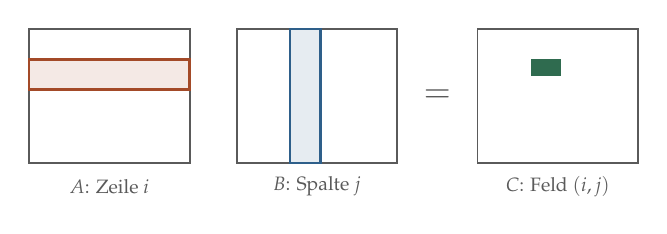
\begin{tikzpicture}[scale=0.85]
\draw[grau, line width=0.7pt] (-3.4,-1.0) rectangle (-1.0,1.0);
\draw[akzent, fill=akzent!12, line width=1pt] (-3.4,0.1) rectangle (-1.0,0.55);
\node[font=\scriptsize, color=grau] at (-2.2,-1.35) {$A$: Zeile $i$};
\draw[grau, line width=0.7pt] (-0.3,-1.0) rectangle (2.1,1.0);
\draw[mittel, fill=mittel!12, line width=1pt] (0.5,-1.0) rectangle (0.95,1.0);
\node[font=\scriptsize, color=grau] at (0.9,-1.35) {$B$: Spalte $j$};
\node[font=\large, color=grau] at (2.7,0) {$=$};
\draw[grau, line width=0.7pt] (3.3,-1.0) rectangle (5.7,1.0);
\fill[gruen] (4.1,0.3) rectangle (4.55,0.55);
\node[font=\scriptsize, color=grau] at (4.5,-1.35) {$C$: Feld $(i,j)$};
\end{tikzpicture}
\end{center}

\begin{center}
\begin{minipage}{0.88\textwidth}
\kursiv{Ein einzelnes Feld des Produkts entsteht also aus einer ganzen Zeile und einer ganzen Spalte. Für die vollständige Matrix braucht man $n^2$ solche Rechnungen mit je $n$ Multiplikationen --- insgesamt $n^3$. Dass es auch schneller geht, ist eine eigene Geschichte; Band 1 der Informatikreihe erzählt sie.}
\end{minipage}
\end{center}
\end{merksatz}

\begin{merksatz}
\boxtitel{$A^2$ für unser Beispiel --- ein Feld vorgerechnet}
Wir berechnen $A^2 = A \cdot A$ für die Matrix von oben.

\schritt{Das Feld $(1,1)$}
Erste Zeile von $A$: $(0,1,1,0,0)$. Erste Spalte von $A$: $(0,1,1,0,0)^{\!\top}$.
\[ 0\cdot 0 + 1\cdot 1 + 1\cdot 1 + 0\cdot 0 + 0\cdot 0 = 0 + 1 + 1 + 0 + 0 = 2 \]

\schritt{Das Feld $(1,4)$}
Erste Zeile von $A$: $(0,1,1,0,0)$. Vierte Spalte von $A$: $(0,1,0,0,1)^{\!\top}$.
\[ 0\cdot 0 + 1\cdot 1 + 1\cdot 0 + 0\cdot 0 + 0\cdot 1 = 1 \]

\schritt{Die vollständige Matrix}
\[ A^2 = \begin{pmatrix}
2 & 1 & 1 & 1 & 1 \\
1 & 3 & 1 & 0 & 2 \\
1 & 1 & 3 & 2 & 0 \\
1 & 0 & 2 & 2 & 0 \\
1 & 2 & 0 & 0 & 2
\end{pmatrix} \]

\schritt{Was fällt auf?}
Der Eintrag $(1,1)$ ist $2$ --- und $\deg(A) = 2$. Der Eintrag $(2,2)$ ist $3$ --- und $\deg(B) = 3$. Auf der Diagonalen stehen die Grade.

Der Eintrag $(1,4)$ ist $1$. Zwischen $A$ und $D$ gibt es keine Kante, aber genau einen Weg der Länge $2$: $A - B - D$.

Der Eintrag $(2,4)$ ist $0$. Zwischen $B$ und $D$ gibt es eine Kante, aber keinen Kantenzug der Länge genau $2$: Man müsste über einen gemeinsamen Nachbarn gehen, und $N(B) = \{A,C,D\}$, $N(D) = \{B,E\}$ haben keinen gemeinsamen Eintrag.
\end{merksatz}

\begin{merksatz}
\boxtitel{Satz 3.4 --- Potenzen der Adjazenzmatrix zählen Kantenzüge}
Sei $A$ die Adjazenzmatrix von $G$ und $k \ge 0$. Dann ist der Eintrag $(A^k)_{ij}$ gleich der Anzahl der Kantenzüge der Länge $k$ von $v_i$ nach $v_j$.
\end{merksatz}

\begin{merksatz}
\boxtitel{Beweis durch Induktion über $k$}
\schritt{Induktionsanfang I: $k = 0$}
$A^0$ ist definitionsgemäß die \Begriff{Einheitsmatrix} $I$ --- Einsen auf der Diagonalen, sonst Nullen.

Wie viele Kantenzüge der Länge $0$ gibt es von $v_i$ nach $v_j$? Ein Kantenzug der Länge $0$ ist eine Folge mit einem einzigen Eintrag, also $(v_i)$; er führt von $v_i$ nach $v_i$. Für $i = j$ gibt es also genau einen, für $i \neq j$ keinen. Das ist genau die Einheitsmatrix.

\schritt{Induktionsanfang II: $k = 1$}
$A^1 = A$. Kantenzüge der Länge $1$ von $v_i$ nach $v_j$ sind genau die Folgen $(v_i, v_j)$ mit $\{v_i,v_j\} \in E$. Davon gibt es einen, wenn die Kante existiert, sonst keinen --- also $a_{ij}$.

\schritt{Induktionsschritt --- die Annahme}
Sei $k \ge 1$ und die Behauptung für $k$ bereits bewiesen. Zu zeigen ist sie für $k+1$.

\schritt{Der entscheidende Gedanke: nach der vorletzten Ecke sortieren}
Jeder Kantenzug der Länge $k+1$ von $v_i$ nach $v_j$ hat die Gestalt
\[ (v_i, \ \ldots \ , v_\ell, \ v_j) \]
für eine Ecke $v_\ell$ --- nämlich die vorletzte. Er zerfällt damit eindeutig in zwei Teile:
\begin{itemize}[leftmargin=1.4em, itemsep=2pt]
\item ein Kantenzug der Länge $k$ von $v_i$ nach $v_\ell$;
\item ein letzter Schritt von $v_\ell$ nach $v_j$, der die Kante $\{v_\ell, v_j\}$ benutzt.
\end{itemize}

\schritt{Die Zählung}
Wir zählen die Kantenzüge der Länge $k+1$, indem wir nach der vorletzten Ecke $v_\ell$ sortieren und die Fälle addieren.

Für ein festes $v_\ell$: Es gibt $(A^k)_{i\ell}$ Möglichkeiten für den ersten Teil (Induktionsannahme). Der letzte Schritt ist möglich, wenn $\{v_\ell,v_j\} \in E$, also in $a_{\ell j}$ Fällen --- das ist $1$ oder $0$. Jede Kombination aus erstem Teil und letztem Schritt ergibt genau einen Kantenzug der Länge $k+1$, und jeder entsteht so genau einmal. Also gibt es für dieses feste $v_\ell$ genau
\[ (A^k)_{i\ell} \cdot a_{\ell j} \]
Kantenzüge.

\schritt{Aufsummieren}
Jeder Kantenzug hat genau eine vorletzte Ecke, wird also bei genau einem $\ell$ gezählt. Summieren über alle $\ell$:
\[ \#\{\text{Kantenzüge der Länge } k+1 \text{ von } v_i \text{ nach } v_j\} \;=\; \sum_{\ell=1}^{n} (A^k)_{i\ell}\, a_{\ell j} . \]

\schritt{Und das ist genau das Matrixprodukt}
Die rechte Seite ist nach Definition 3.3 der Eintrag $(i,j)$ des Produkts $A^k \cdot A = A^{k+1}$. $\blacksquare$
\end{merksatz}

\begin{warnung}
\boxtitelr{Der Satz zählt Kantenzüge, nicht Wege}
Das ist keine Kleinigkeit. Im Beispiel ist $(A^2)_{22} = 3$. Es gibt aber keinen \kursiv{Weg} der Länge $2$ von $B$ nach $B$ --- Wege haben lauter verschiedene Ecken. Was gezählt wird, sind die drei Kantenzüge
\[ (B,A,B), \quad (B,C,B), \quad (B,D,B) . \]
Sie laufen jeweils hin und zurück.

\begin{center}
\begin{minipage}{0.88\textwidth}
\kursiv{Es gibt keine ähnlich einfache Formel für die Anzahl der \kursiv{Wege} einer gegebenen Länge. Die Rechnung mit Matrixpotenzen funktioniert nur deshalb so glatt, weil Kantenzüge sich beliebig zerlegen und zusammensetzen lassen --- bei Wegen muss man dabei prüfen, ob sich Ecken wiederholen, und genau das lässt sich nicht in ein Produkt fassen.}
\end{minipage}
\end{center}
\end{warnung}

\begin{merksatz}
\boxtitel{Folgerung 3.5 --- Dreiecke zählen}
Die Anzahl der Dreiecke in $G$ ist
\[ \frac{1}{6} \operatorname{spur}(A^3), \]
wobei $\operatorname{spur}$ die Summe der Diagonaleinträge bezeichnet.

\schritt{Warum}
$(A^3)_{ii}$ zählt die geschlossenen Kantenzüge der Länge $3$ von $v_i$ nach $v_i$. Ein solcher Kantenzug $(v_i, x, y, v_i)$ verlangt drei Kanten $\{v_i,x\}$, $\{x,y\}$, $\{y,v_i\}$. Wegen $x \neq v_i$ (keine Schlingen) und $y \neq x$ und $y \neq v_i$ sind alle drei Ecken verschieden --- es ist stets ein Dreieck.

\schritt{Warum $\frac{1}{6}$}
Jedes Dreieck mit den Ecken $p,q,r$ wird gezählt: bei $i = p$, bei $i = q$ und bei $i = r$ --- das sind $3$ Startpunkte. Und von jedem Startpunkt aus in zwei Richtungen --- also $3 \cdot 2 = 6$ Mal insgesamt.

\schritt{Probe am Beispiel}
Unser Dienstplangraph enthält genau ein Dreieck, nämlich $A,B,C$. Es müsste also $\operatorname{spur}(A^3) = 6$ sein.

Wir brauchen nur die Diagonale von $A^3 = A^2 \cdot A$. Für $(A^3)_{11}$: erste Zeile von $A^2$ ist $(2,1,1,1,1)$, erste Spalte von $A$ ist $(0,1,1,0,0)^{\!\top}$:
\[ 2\cdot 0 + 1\cdot 1 + 1\cdot 1 + 1\cdot 0 + 1\cdot 0 = 2 . \]
Ebenso $(A^3)_{22}$: Zeile $(1,3,1,0,2)$ mal Spalte $(1,0,1,1,0)^{\!\top}$ ergibt $1 + 0 + 1 + 0 + 0 = 2$.
Und $(A^3)_{33}$: Zeile $(1,1,3,2,0)$ mal Spalte $(1,1,0,0,1)^{\!\top}$ ergibt $1+1+0+0+0 = 2$.
Für $(A^3)_{44}$: Zeile $(1,0,2,2,0)$ mal Spalte $(0,1,0,0,1)^{\!\top}$ ergibt $0+0+0+0+0 = 0$.
Für $(A^3)_{55}$: Zeile $(1,2,0,0,2)$ mal Spalte $(0,0,1,1,0)^{\!\top}$ ergibt $0+0+0+0+0 = 0$.

\[ \operatorname{spur}(A^3) = 2+2+2+0+0 = 6, \qquad \frac{6}{6} = 1 . \quad \checkmark \]

Die Nullen bei $D$ und $E$ sagen genau das Richtige: Diese beiden Ecken liegen auf keinem Dreieck.
\end{merksatz}

\section{Inzidenzmatrix und Adjazenzliste}

\begin{definition}
\boxtitelm{Definition 3.6 --- Inzidenzmatrix}
Sind die Ecken als $v_1, \ldots, v_n$ und die Kanten als $e_1, \ldots, e_m$ nummeriert, so ist die \Begriff{Inzidenzmatrix} $B$ die $n \times m$-Matrix mit
\[ b_{ij} = \begin{cases} 1, & \text{falls } v_i \text{ auf } e_j \text{ liegt}, \\ 0, & \text{sonst.} \end{cases} \]
\end{definition}

\begin{merksatz}
\boxtitel{Ihre auffälligste Eigenschaft}
In jeder \kursiv{Spalte} stehen genau zwei Einsen --- eine Kante hat zwei Enden. In jeder \kursiv{Zeile} stehen $\deg(v_i)$ Einsen.

Zählt man alle Einsen einmal spaltenweise und einmal zeilenweise, so erhält man
\[ 2m \quad \text{beziehungsweise} \quad \sum_i \deg(v_i) . \]
Das ist wieder das Handschlaglemma --- diesmal so unmittelbar, dass der Beweis in einem Satz steht. Die Inzidenzmatrix \kursiv{ist} die Tabelle der Inzidenzen, die in Kapitel~1 gezählt wurden.
\end{merksatz}

\begin{definition}
\boxtitelm{Definition 3.7 --- Adjazenzliste}
Die \Begriff{Adjazenzliste} von $G$ ist die Zuordnung, die jeder Ecke $v$ die Liste ihrer Nachbarn $N(v)$ zuordnet.
\end{definition}

\begin{merksatz}
\boxtitel{Der Vergleich}
\begin{center}
{\small
\renewcommand{\arraystretch}{1.5}
\begin{tabular}{@{}P{2.4cm}P{2.0cm}P{2.2cm}P{2.0cm}@{}}
\toprule
& \textbf{Adjazenz\-matrix} & \textbf{Inzidenz\-matrix} & \textbf{Adjazenz\-liste}\\
\midrule
Platzbedarf & $n^2$ & $n \cdot m$ & $2m$\\
\enquote{Sind $u,v$ benachbart?} & \textcolor{gruen}{sofort} & \textcolor{akzent}{langsam} & $\deg(u)$ Schritte\\
\enquote{Alle Nachbarn von $u$?} & $n$ Schritte & \textcolor{akzent}{$m$ Schritte} & \textcolor{gruen}{sofort}\\
Rechnen & \textcolor{gruen}{Satz 3.4} & Sätze über Flüsse & \textcolor{akzent}{kaum}\\
\bottomrule
\end{tabular}}
\end{center}

\begin{center}
\begin{minipage}{0.88\textwidth}
\kursiv{Für einen Graphen mit $n = 10^6$ Ecken und $m = 5 \cdot 10^6$ Kanten bräuchte die Adjazenzmatrix $10^{12}$ Felder --- unmöglich. Die Adjazenzliste kommt mit $10^7$ Einträgen aus. Solche Graphen heißen \Begriff{dünn}: Sie haben viel weniger Kanten, als möglich wären.}
\end{minipage}
\end{center}
\end{merksatz}

\section{Übungsaufgaben}

\begin{aufgabe}
\boxtitel{Aufgabe 3.1 --- Vom Bild zur Matrix und zurück}
Gegeben sei die Matrix
\[ A = \begin{pmatrix}
0 & 1 & 0 & 1 \\
1 & 0 & 1 & 1 \\
0 & 1 & 0 & 1 \\
1 & 1 & 1 & 0
\end{pmatrix} . \]
Bestimmen Sie Kantenzahl, Gradfolge und die Anzahl der Dreiecke.

\loesung
\schritt{Schritt 1 --- Prüfung, ob es überhaupt eine Adjazenzmatrix sein kann}
Diagonale: alle Einträge $0$ --- keine Schlingen. \checkmark\\
Symmetrie: $a_{12} = a_{21} = 1$, $a_{13} = a_{31} = 0$, $a_{14} = a_{41} = 1$, $a_{23} = a_{32} = 1$, $a_{24} = a_{42} = 1$, $a_{34} = a_{43} = 1$. \checkmark

\schritt{Schritt 2 --- Grade als Zeilensummen}
\begin{center}
\renewcommand{\arraystretch}{1.4}
\begin{tabular}{@{}P{1.4cm}P{2.6cm}P{1.4cm}@{}}
\toprule
\textbf{Zeile} & \textbf{Einträge} & $\deg$\\
\midrule
$1$ & $0+1+0+1$ & $2$\\
$2$ & $1+0+1+1$ & $3$\\
$3$ & $0+1+0+1$ & $2$\\
$4$ & $1+1+1+0$ & $3$\\
\bottomrule
\end{tabular}
\end{center}
Gradfolge: $(3,3,2,2)$.

\schritt{Schritt 3 --- Kantenzahl}
Nach Satz 1.3: $m = \frac{2+3+2+3}{2} = \frac{10}{2} = 5$.

\schritt{Schritt 4 --- Die Kanten benennen}
Aus den Einsen oberhalb der Diagonalen: $\{1,2\}$, $\{1,4\}$, $\{2,3\}$, $\{2,4\}$, $\{3,4\}$. Das sind fünf. \checkmark

\schritt{Schritt 5 --- Das Bild}
\begin{center}
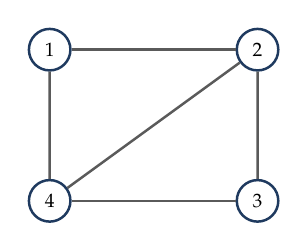
\begin{tikzpicture}[scale=1.2]
\node[knotenb] (1) at (-1.1,0.8) {$1$};
\node[knotenb] (2) at (1.1,0.8) {$2$};
\node[knotenb] (3) at (1.1,-0.8) {$3$};
\node[knotenb] (4) at (-1.1,-0.8) {$4$};
\draw[kante] (1)--(2); \draw[kante] (1)--(4); \draw[kante] (2)--(3);
\draw[kante] (2)--(4); \draw[kante] (3)--(4);
\end{tikzpicture}
\end{center}

\schritt{Schritt 6 --- Dreiecke}
Direkt abgelesen: $\{1,2,4\}$ ist ein Dreieck (die Kanten $12$, $24$, $41$ sind alle da). $\{2,3,4\}$ ebenfalls. $\{1,2,3\}$ nicht, denn $13$ fehlt. $\{1,3,4\}$ nicht, denn $13$ fehlt. Also \textbf{zwei} Dreiecke.

\schritt{Probe über Folgerung 3.5}
Wir brauchen $\operatorname{spur}(A^3)$, das sollte $6 \cdot 2 = 12$ sein.

Zunächst $A^2$. Zeile $1$ von $A$ ist $(0,1,0,1)$.
\begin{align*}
(A^2)_{11} &= (0,1,0,1)\cdot(0,1,0,1) = 0+1+0+1 = 2\\
(A^2)_{12} &= (0,1,0,1)\cdot(1,0,1,1) = 0+0+0+1 = 1\\
(A^2)_{13} &= (0,1,0,1)\cdot(0,1,0,1) = 0+1+0+1 = 2\\
(A^2)_{14} &= (0,1,0,1)\cdot(1,1,1,0) = 0+1+0+0 = 1
\end{align*}
Auf dieselbe Weise erhält man
\[ A^2 = \begin{pmatrix} 2 & 1 & 2 & 1 \\ 1 & 3 & 1 & 2 \\ 2 & 1 & 2 & 1 \\ 1 & 2 & 1 & 3 \end{pmatrix}. \]

Nun die Diagonale von $A^3$:
\begin{align*}
(A^3)_{11} &= (2,1,2,1)\cdot(0,1,0,1) = 0+1+0+1 = 2\\
(A^3)_{22} &= (1,3,1,2)\cdot(1,0,1,1) = 1+0+1+2 = 4\\
(A^3)_{33} &= (2,1,2,1)\cdot(0,1,0,1) = 0+1+0+1 = 2\\
(A^3)_{44} &= (1,2,1,3)\cdot(1,1,1,0) = 1+2+1+0 = 4
\end{align*}
\[ \operatorname{spur}(A^3) = 2+4+2+4 = 12, \qquad \frac{12}{6} = 2 . \quad \checkmark \]

Die Zahlen sagen sogar mehr: Die Ecken $2$ und $4$ liegen auf je zwei Dreiecken ($4/2 = 2$), die Ecken $1$ und $3$ auf je einem.
\end{aufgabe}

\begin{aufgabe}
\boxtitel{Aufgabe 3.2 --- Kantenzüge zählen}
Wie viele Kantenzüge der Länge $4$ gibt es im Kreis $C_4$ von einer Ecke zu sich selbst?

\loesung
\schritt{Schritt 1 --- Die Matrix}
$C_4$ mit den Ecken $1,2,3,4$ im Kreis hat die Kanten $12$, $23$, $34$, $41$:
\[ A = \begin{pmatrix} 0&1&0&1 \\ 1&0&1&0 \\ 0&1&0&1 \\ 1&0&1&0 \end{pmatrix} \]

\schritt{Schritt 2 --- $A^2$}
Zeile $1$ ist $(0,1,0,1)$.
\[ (A^2)_{11} = (0,1,0,1)\cdot(0,1,0,1) = 2, \quad (A^2)_{12} = (0,1,0,1)\cdot(1,0,1,0) = 0, \]
\[ (A^2)_{13} = (0,1,0,1)\cdot(0,1,0,1) = 2, \quad (A^2)_{14} = (0,1,0,1)\cdot(1,0,1,0) = 0 . \]
Aus Symmetriegründen ergibt sich
\[ A^2 = \begin{pmatrix} 2&0&2&0 \\ 0&2&0&2 \\ 2&0&2&0 \\ 0&2&0&2 \end{pmatrix} = 2 \begin{pmatrix} 1&0&1&0 \\ 0&1&0&1 \\ 1&0&1&0 \\ 0&1&0&1 \end{pmatrix}. \]

\schritt{Schritt 3 --- $A^4 = (A^2)^2$}
Statt zweimal weiterzumultiplizieren, quadrieren wir $A^2$. Nennen wir $M$ die Matrix in der Klammer, also $A^2 = 2M$. Dann ist
\[ A^4 = (2M)^2 = 4 M^2 . \]
Für $M^2$: Zeile $1$ von $M$ ist $(1,0,1,0)$.
\[ (M^2)_{11} = (1,0,1,0)\cdot(1,0,1,0) = 2, \qquad (M^2)_{12} = (1,0,1,0)\cdot(0,1,0,1) = 0 . \]
Also $M^2 = 2M$ und damit
\[ A^4 = 4 \cdot 2M = 8M, \qquad (A^4)_{11} = 8 . \]

\schritt{Antwort}
Es gibt $\mathbf{8}$ geschlossene Kantenzüge der Länge $4$ von einer Ecke zu sich selbst.

\schritt{Probe durch Aufzählen}
Wir starten in Ecke $1$; die Nachbarn sind $2$ und $4$. Wir schreiben alle Möglichkeiten auf, wobei nach vier Schritten wieder $1$ erreicht sein muss:
\begin{center}
{\small
\renewcommand{\arraystretch}{1.35}
\begin{tabular}{@{}P{2.6cm}P{2.6cm}@{}}
\toprule
$1,2,1,2,1$ & $1,4,1,4,1$\\
$1,2,1,4,1$ & $1,4,1,2,1$\\
$1,2,3,2,1$ & $1,4,3,4,1$\\
$1,2,3,4,1$ & $1,4,3,2,1$\\
\bottomrule
\end{tabular}}
\end{center}
Acht Stück. \checkmark

\begin{center}
\begin{minipage}{0.86\textwidth}
\kursiv{Nur die beiden letzten in der Liste --- $1,2,3,4,1$ und $1,4,3,2,1$ --- sind Kreise. Die übrigen sechs enthalten ein Hin und Zurück. Das ist der Unterschied zwischen Kantenzug und Kreis, an einem Beispiel abgezählt.}
\end{minipage}
\end{center}
\end{aufgabe}

\begin{aufgabe}
\boxtitel{Aufgabe 3.3 --- Zusammenhang aus der Matrix ablesen}
Zeigen Sie: Ein Graph mit $n$ Ecken ist genau dann zusammenhängend, wenn in der Matrix
\[ S = I + A + A^2 + \cdots + A^{n-1} \]
kein Eintrag gleich $0$ ist.

\loesung
\schritt{Schritt 1 --- Was $S_{ij}$ bedeutet}
Nach Satz 3.4 ist $(A^k)_{ij}$ die Anzahl der Kantenzüge der Länge $k$ von $v_i$ nach $v_j$. Also ist
\[ S_{ij} = \sum_{k=0}^{n-1} (A^k)_{ij} \]
die Anzahl aller Kantenzüge von $v_i$ nach $v_j$ mit Länge \kursiv{höchstens} $n-1$.

Da alle Summanden $\ge 0$ sind, gilt:
\[ S_{ij} > 0 \iff \text{es gibt einen Kantenzug von } v_i \text{ nach } v_j \text{ der Länge} \le n-1 . \]

\schritt{Schritt 2 --- Richtung 1: alle Einträge positiv $\Longrightarrow$ zusammenhängend}
Sind alle $S_{ij} > 0$, so gibt es zwischen je zwei Ecken einen Kantenzug, nach Lemma 2.3 also einen Weg. Das ist Definition 2.4.

\schritt{Schritt 3 --- Richtung 2: zusammenhängend $\Longrightarrow$ alle Einträge positiv}
Sei $G$ zusammenhängend und $v_i, v_j$ beliebig. Es gibt einen Weg von $v_i$ nach $v_j$.

Entscheidend ist nun die Längenschranke. Ein Weg hat lauter verschiedene Ecken. Es gibt nur $n$ Ecken, also hat ein Weg höchstens $n$ Eckeneinträge und damit höchstens $n-1$ Schritte. Seine Länge $k$ erfüllt somit $0 \le k \le n-1$.

Damit trägt dieser Weg zum Summanden $A^k$ mit $k \le n-1$ bei, und $S_{ij} \ge 1 > 0$. $\blacksquare$

\schritt{Warum die Schranke $n-1$ genau richtig ist}
Sie kann nicht kleiner gewählt werden: Im Weg $P_n$ ist der Abstand der beiden Endecken genau $n-1$. Mit $S = I + A + \cdots + A^{n-2}$ bliebe dieser Eintrag $0$, und das Kriterium würde einen zusammenhängenden Graphen fälschlich ablehnen.
\end{aufgabe}

\begin{geschichte}
\boxtitelg{Kirchhoff und die erste Rechnung mit Graphen}
\Person{Gustav Robert Kirchhoff} veröffentlichte 1847 eine Arbeit über die Verteilung elektrischer Ströme in verzweigten Leitern. Um die Gleichungen aufzustellen, brauchte er eine Buchführung darüber, welcher Leiter welche Knoten verbindet --- und schrieb damit die erste Inzidenzmatrix der Geschichte hin, achtzig Jahre bevor jemand das Wort \enquote{Matrix} in diesem Zusammenhang benutzte.

Kirchhoff ging weiter: Er zeigte, dass die unabhängigen Gleichungen den Kreisen des Netzwerks entsprechen und dass ihre Anzahl $m - n + 1$ beträgt. Diese Zahl heißt heute die \Begriff{zyklomatische Zahl} des Graphen. Sie wird in Kapitel~4 wieder auftauchen, wo sie als \enquote{Anzahl der Kanten, die man über einen Spannbaum hinaus hat} eine anschauliche Bedeutung bekommt.

\begin{center}
\begin{minipage}{0.9\textwidth}
\kursiv{Bemerkenswert ist, dass Kirchhoff die Graphentheorie nicht suchte. Er brauchte sie, um ein physikalisches Problem zu lösen. Das ist der Regelfall in der Geschichte dieses Gebiets: Fast jeder Grundbegriff wurde von jemandem eingeführt, der etwas ganz anderes vorhatte.}
\end{minipage}
\end{center}
\end{geschichte}

\begin{merksatz}
\boxtitel{Was Sie jetzt können}
\begin{center}
\renewcommand{\arraystretch}{1.5}
\begin{tabular}{@{}P{3.0cm}P{5.6cm}@{}}
\toprule
\textbf{Drei Darstellungen} & Adjazenzmatrix, Inzidenzmatrix, Adjazenzliste --- und wann welche\\
\textbf{Satz 3.4} & $(A^k)_{ij}$ zählt Kantenzüge der Länge $k$\\
\textbf{Folgerung 3.5} & Dreiecke über $\frac{1}{6}\operatorname{spur}(A^3)$\\
\textbf{Zusammenhang} & aus $I + A + \cdots + A^{n-1}$ ablesbar\\
\bottomrule
\end{tabular}
\end{center}

\begin{center}
\begin{minipage}{0.88\textwidth}
\kursiv{Damit ist Teil~I abgeschlossen. Ab Kapitel~4 geht es nicht mehr um Begriffe, sondern um Struktur: Wie sehen die Graphen aus, die mit möglichst wenigen Kanten zusammenhängend sind?}
\end{minipage}
\end{center}
\end{merksatz}

\part{Bäume}

\chapter{Bäume und Wälder}

\section{Die sparsamste Verbindung}

Satz 2.8 hat gezeigt: Ein zusammenhängender Graph mit $n$ Ecken braucht mindestens $n-1$ Kanten. Und der Weg $P_n$ zeigt, dass $n-1$ auch genügen kann.

Damit stellt sich die Frage nach den Graphen, die diese Schranke genau erreichen: den sparsamsten unter allen, die noch zusammenhängen. Sie heißen Bäume, sie sind der wichtigste Einzelbegriff dieses Bandes, und sie kommen an mehr Stellen vor, als man erwartet.

\begin{merksatz}
\boxtitel{Wo Bäume auftreten}
\begin{center}
{\small
\renewcommand{\arraystretch}{1.45}
\begin{tabular}{@{}P{3.0cm}P{5.4cm}@{}}
\toprule
\textbf{Alarmierungs\-kette} & Jede Person ruft zwei weitere an. Niemand wird doppelt angerufen, niemand vergessen.\\
\textbf{Organigramm} & Jede Stelle hat genau eine vorgesetzte Stelle, die Klinikleitung keine.\\
\textbf{Diagnose\-algorithmus} & Jede Frage verzweigt; von der Eingangsfrage zu jeder Diagnose führt genau ein Weg.\\
\textbf{Stammbaum} & Abstammungsverhältnisse ohne Rückverbindungen.\\
\textbf{Datei\-verzeichnis} & Jede Datei liegt in genau einem Ordner.\\
\bottomrule
\end{tabular}}
\end{center}

\begin{center}
\begin{minipage}{0.88\textwidth}
\kursiv{Das Gemeinsame steht in der dritten Zeile: \enquote{genau ein Weg}. Das ist keine Zufallseigenschaft, sondern eine der fünf gleichwertigen Beschreibungen, die Satz 4.2 aufstellt.}
\end{minipage}
\end{center}
\end{merksatz}

\begin{definition}
\boxtitelm{Definition 4.1 --- Baum, Wald, Blatt}
\begin{itemize}[leftmargin=1.4em, itemsep=4pt]
\item Ein \Begriff{Baum} ist ein Graph, der zusammenhängend und kreisfrei ist.
\item Ein \Begriff{Wald} ist ein Graph, der kreisfrei ist. (Er darf also in mehrere Komponenten zerfallen; jede davon ist dann ein Baum --- daher der Name.)
\item Eine Ecke vom Grad $1$ heißt \Begriff{Blatt}.
\end{itemize}
\end{definition}

\begin{merksatz}
\boxtitel{Alle Bäume mit bis zu fünf Ecken}
\begin{center}
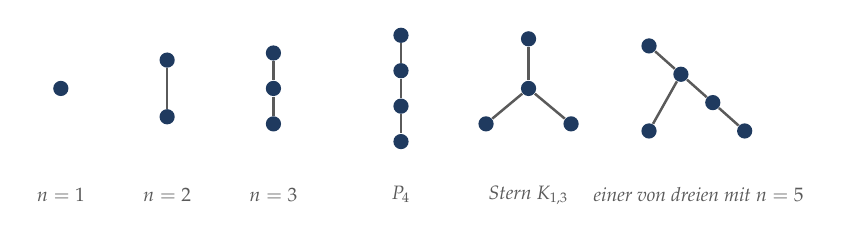
\begin{tikzpicture}[scale=0.9]
\begin{scope}
\node[knoten] (a) at (0,0) {};
\node[font=\scriptsize\itshape, color=grau] at (0,-1.5) {$n=1$};
\end{scope}
\begin{scope}[xshift=1.5cm]
\node[knoten] (b1) at (0,0.4) {};
\node[knoten] (b2) at (0,-0.4) {};
\draw[kante] (b1)--(b2);
\node[font=\scriptsize\itshape, color=grau] at (0,-1.5) {$n=2$};
\end{scope}
\begin{scope}[xshift=3.0cm]
\node[knoten] (c1) at (0,0.5) {};
\node[knoten] (c2) at (0,0) {};
\node[knoten] (c3) at (0,-0.5) {};
\draw[kante] (c1)--(c2); \draw[kante] (c2)--(c3);
\node[font=\scriptsize\itshape, color=grau] at (0,-1.5) {$n=3$};
\end{scope}
\begin{scope}[xshift=4.8cm]
\node[knoten] (d1) at (0,0.75) {};
\node[knoten] (d2) at (0,0.25) {};
\node[knoten] (d3) at (0,-0.25) {};
\node[knoten] (d4) at (0,-0.75) {};
\draw[kante] (d1)--(d2); \draw[kante] (d2)--(d3); \draw[kante] (d3)--(d4);
\node[font=\scriptsize\itshape, color=grau] at (0,-1.5) {$P_4$};
\end{scope}
\begin{scope}[xshift=6.6cm]
\node[knoten] (e0) at (0,0) {};
\node[knoten] (e1) at (0,0.7) {};
\node[knoten] (e2) at (-0.6,-0.5) {};
\node[knoten] (e3) at (0.6,-0.5) {};
\draw[kante] (e0)--(e1); \draw[kante] (e0)--(e2); \draw[kante] (e0)--(e3);
\node[font=\scriptsize\itshape, color=grau] at (0,-1.5) {Stern $K_{1,3}$};
\end{scope}
\begin{scope}[xshift=9.0cm]
\node[knoten] (f1) at (-0.7,0.6) {};
\node[knoten] (f2) at (-0.25,0.2) {};
\node[knoten] (f3) at (0.2,-0.2) {};
\node[knoten] (f4) at (0.65,-0.6) {};
\node[knoten] (f5) at (-0.7,-0.6) {};
\draw[kante] (f1)--(f2); \draw[kante] (f2)--(f3); \draw[kante] (f3)--(f4); \draw[kante] (f2)--(f5);
\node[font=\scriptsize\itshape, color=grau] at (0,-1.5) {einer von dreien mit $n=5$};
\end{scope}
\end{tikzpicture}
\end{center}

Für $n = 1,2,3,4,5$ gibt es genau $1, 1, 1, 2, 3$ verschiedene Bäume (bis auf Isomorphie). Die Zahlen wachsen danach schnell: $6, 11, 23, 47, 106$ für $n = 6, \ldots, 10$. Eine geschlossene Formel dafür ist nicht bekannt --- Abschnitt 5.4 kommt darauf zurück.
\end{merksatz}

\section{Fünf Beschreibungen, die dasselbe bedeuten}

\begin{merksatz}
\boxtitel{Satz 4.2 --- Charakterisierung der Bäume}
Für einen Graphen $T$ mit $n$ Ecken und $m$ Kanten sind die folgenden fünf Aussagen gleichwertig:
\begin{center}
\renewcommand{\arraystretch}{1.55}
\begin{tabular}{@{}P{1.0cm}P{7.4cm}@{}}
\toprule
(i) & $T$ ist ein Baum --- also zusammenhängend und kreisfrei.\\
(ii) & Je zwei Ecken sind durch \kursiv{genau einen} Weg verbunden.\\
(iii) & $T$ ist zusammenhängend und $m = n-1$.\\
(iv) & $T$ ist kreisfrei und $m = n-1$.\\
(v) & $T$ ist zusammenhängend, und jede Kante ist eine Brücke.\\
\bottomrule
\end{tabular}
\end{center}
\end{merksatz}

\begin{merksatz}
\boxtitel{Wie man fünf Aussagen als gleichwertig nachweist}
\enquote{Gleichwertig} heißt: Gilt eine von ihnen, so gelten alle. Streng genommen wären $5 \cdot 4 = 20$ Folgerungen zu zeigen --- von jeder zu jeder anderen.

Es geht sparsamer. Man zeigt einen \Begriff{Ringschluss}:
\[ \text{(i)} \Rightarrow \text{(ii)} \Rightarrow \text{(iii)} \Rightarrow \text{(iv)} \Rightarrow \text{(v)} \Rightarrow \text{(i)} \]
Das sind fünf Beweise statt zwanzig. Warum genügt das? Weil man von jeder Aussage zu jeder anderen gelangt, indem man im Ring weiterläuft --- notfalls einmal ganz herum.

\begin{center}
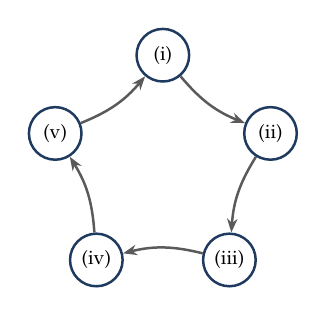
\begin{tikzpicture}[scale=1.15]
\foreach \i/\lab in {0/{(i)}, 1/{(ii)}, 2/{(iii)}, 3/{(iv)}, 4/{(v)}} {
  \node[knotenb, minimum size=19pt] (r\i) at (90-72*\i:1.25) {\lab};
}
\foreach \i/\j in {0/1,1/2,2/3,3/4,4/0}
  \draw[kante, -{Stealth[length=5pt]}] (r\i) to[bend right=14] (r\j);
\end{tikzpicture}
\end{center}
\end{merksatz}

\begin{merksatz}
\boxtitel{Beweis, Teil 1: (i) $\Rightarrow$ (ii)}
Sei $T$ zusammenhängend und kreisfrei, seien $u,v$ Ecken.

\schritt{Es gibt mindestens einen Weg}
Das ist genau die Definition des Zusammenhangs (Definition 2.4).

\schritt{Es gibt höchstens einen --- Annahme}
Angenommen, es gäbe zwei \kursiv{verschiedene} Wege $P$ und $Q$ von $u$ nach $v$.

\schritt{Die erste Abweichung finden}
Beide beginnen bei $u$. Wir laufen sie gleichzeitig ab. Da sie verschieden sind, gibt es eine erste Stelle, an der sie sich unterscheiden. Sei $x$ die letzte Ecke, bis zu der beide übereinstimmen; danach benutzt $P$ eine Kante $\{x, p\}$ und $Q$ eine Kante $\{x, q\}$ mit $p \neq q$.

\schritt{Die erste Wiedervereinigung finden}
Beide Wege enden bei $v$, treffen sich also wieder. Wir laufen $P$ ab $x$ weiter und schauen, welche Ecke von $P$ als erste wieder auf $Q$ liegt; sei $y$ diese Ecke. Sie existiert, weil spätestens $v$ auf beiden liegt. Und es ist $y \neq x$, denn $y$ liegt hinter $x$ auf $P$ und $P$ hat lauter verschiedene Ecken.

\begin{center}
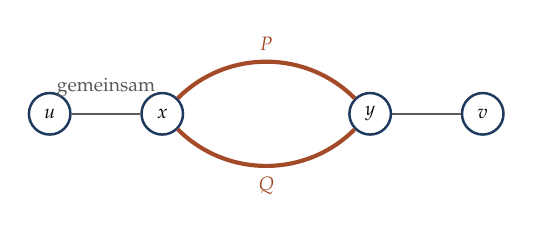
\begin{tikzpicture}[scale=1.1]
\node[knotenb] (u) at (-2.2,0) {$u$};
\node[knotenb] (x) at (-0.9,0) {$x$};
\node[knotenb] (y) at (1.5,0) {$y$};
\node[knotenb] (v) at (2.8,0) {$v$};
\draw[kante] (u) -- (x);
\draw[kante] (y) -- (v);
\draw[kanted] (x) to[bend left=45] node[above, font=\scriptsize, color=akzent] {$P$} (y);
\draw[kanted] (x) to[bend right=45] node[below, font=\scriptsize, color=akzent] {$Q$} (y);
\node[font=\scriptsize, color=grau] at (-1.55,0.3) {gemeinsam};
\end{tikzpicture}
\end{center}

\schritt{Der Kreis}
Der Abschnitt von $x$ nach $y$ auf $P$ und der Abschnitt von $x$ nach $y$ auf $Q$ haben --- nach Wahl von $x$ und $y$ --- außer $x$ und $y$ selbst keine gemeinsame Ecke. Beide haben Länge $\ge 1$, und mindestens einer hat Länge $\ge 2$: Hätten beide die Länge $1$, so wären es dieselbe Kante $\{x,y\}$, und dann wäre $p = y = q$ im Widerspruch zu $p \neq q$.

Setzt man beide Abschnitte zusammen --- den einen hin, den anderen zurück ---, so entsteht ein geschlossener Kantenzug der Länge $\ge 3$, dessen Ecken bis auf Anfang und Ende verschieden sind. Das ist ein Kreis.

\schritt{Widerspruch}
$T$ war kreisfrei. Also war die Annahme falsch, und es gibt höchstens einen Weg.
\end{merksatz}

\begin{merksatz}
\boxtitel{Beweis, Teil 2: (ii) $\Rightarrow$ (iii)}
\schritt{Zusammenhang}
Aus (ii) folgt sofort: Zwischen je zwei Ecken gibt es einen Weg. Also ist $T$ zusammenhängend.

\schritt{Die Kantenzahl --- Induktion über $n$}
\textbf{Anfang $n=1$:} Ein Graph mit einer Ecke hat keine Kanten, und $n - 1 = 0$. \checkmark

\textbf{Schritt.} Sei $n \ge 2$ und die Behauptung für alle kleineren Eckenzahlen bewiesen. Da $T$ zusammenhängend ist und $n \ge 2$, gibt es mindestens eine Kante; wähle eine, etwa $e = \{x,y\}$.

\schritt{$e$ ist eine Brücke}
Die Kante $e$ selbst ist ein Weg der Länge $1$ von $x$ nach $y$. Nach (ii) ist er der einzige. Läge $e$ auf einem Kreis, so gäbe es nach dem Beweis von Satz 2.14 einen zweiten Weg von $x$ nach $y$ --- den Rest des Kreises. Also liegt $e$ auf keinem Kreis und ist nach Satz 2.14 eine Brücke.

\schritt{$T - e$ hat genau zwei Komponenten}
Mindestens zwei, weil $e$ eine Brücke ist. Höchstens zwei, denn: Sei $w$ eine beliebige Ecke. In $T$ gibt es einen Weg von $w$ nach $x$. Benutzt er $e$ nicht, so liegt $w$ in derselben Komponente von $T-e$ wie $x$. Benutzt er $e$, so muss $e$ der letzte Schritt sein (der Weg endet ja in $x$, und $e$ kommt höchstens einmal vor) --- der Weg läuft also von $w$ nach $y$ ohne $e$ und dann über $e$ nach $x$. Dann liegt $w$ in der Komponente von $y$.

Jede Ecke liegt somit in der Komponente von $x$ oder in der von $y$. Genau zwei.

\schritt{Die Induktionsannahme anwenden}
Seien $T_1$ und $T_2$ diese Komponenten, mit $n_1$ bzw.\ $n_2$ Ecken und $m_1$ bzw.\ $m_2$ Kanten. Es ist $n_1 + n_2 = n$ und $m_1 + m_2 = m - 1$.

Beide erfüllen (ii): Ein Weg zwischen zwei Ecken einer Komponente von $T-e$ ist auch ein Weg in $T$, und ein zweiter dort gäbe einen zweiten in $T$. Beide haben weniger als $n$ Ecken (denn beide sind nichtleer). Nach Induktionsannahme ist $m_1 = n_1 - 1$ und $m_2 = n_2 - 1$.

\schritt{Zusammenrechnen}
\[ m = m_1 + m_2 + 1 = (n_1 - 1) + (n_2 - 1) + 1 = n_1 + n_2 - 1 = n - 1 . \]
\end{merksatz}

\begin{merksatz}
\boxtitel{Beweis, Teil 3: (iii) $\Rightarrow$ (iv)}
Zu zeigen ist nur die Kreisfreiheit; die Kantenzahl ist gegeben.

\schritt{Annahme}
Angenommen, $T$ enthielte einen Kreis $C$. Sei $e$ eine Kante von $C$.

\schritt{Entfernen}
Nach Satz 2.14 ist $e$ keine Brücke, denn $e$ liegt auf einem Kreis. Also hat $T - e$ dieselbe Komponentenzahl wie $T$, ist also weiterhin zusammenhängend.

\schritt{Der Widerspruch}
$T-e$ ist zusammenhängend mit $n$ Ecken und $m - 1 = n - 2$ Kanten. Nach Satz 2.8 braucht ein zusammenhängender Graph mit $n$ Ecken aber mindestens $n-1$ Kanten. Aus $n-2 \ge n-1$ folgt $-2 \ge -1$ --- falsch.

Also gibt es keinen Kreis.
\end{merksatz}

\begin{merksatz}
\boxtitel{Beweis, Teil 4: (iv) $\Rightarrow$ (v)}
\schritt{Schritt 1 --- die Komponenten sind Bäume}
$T$ ist kreisfrei. Jede Zusammenhangskomponente von $T$ ist zusammenhängend (nach Definition) und kreisfrei (ein Kreis in einer Komponente wäre einer in $T$). Also ist jede Komponente ein Baum, erfüllt also (i).

\schritt{Schritt 2 --- ihre Kantenzahlen}
Die Folgerungen (i) $\Rightarrow$ (ii) $\Rightarrow$ (iii) sind bereits bewiesen. Also gilt für jede Komponente $T_i$ mit $n_i$ Ecken und $m_i$ Kanten
\[ m_i = n_i - 1 . \]

\schritt{Schritt 3 --- aufsummieren}
Hat $T$ genau $c$ Komponenten, so ist
\[ m = \sum_{i=1}^{c} m_i = \sum_{i=1}^{c} (n_i - 1) = \Bigl(\sum_{i=1}^{c} n_i\Bigr) - c = n - c . \]

\schritt{Schritt 4 --- $c$ bestimmen}
Nach Voraussetzung ist $m = n-1$. Aus $n - c = n - 1$ folgt $c = 1$. Also ist $T$ zusammenhängend.

\schritt{Schritt 5 --- jede Kante ist Brücke}
$T$ ist kreisfrei, also liegt keine Kante auf einem Kreis. Nach Satz 2.14 ist damit jede Kante eine Brücke.
\end{merksatz}

\begin{merksatz}
\boxtitel{Beweis, Teil 5: (v) $\Rightarrow$ (i)}
$T$ ist nach Voraussetzung zusammenhängend. Zu zeigen bleibt die Kreisfreiheit.

Läge eine Kante $e$ auf einem Kreis, so wäre $e$ nach Satz 2.14 keine Brücke --- im Widerspruch zu (v), wonach \kursiv{jede} Kante eine Brücke ist.

Also gibt es keinen Kreis, und $T$ ist ein Baum. $\blacksquare$

\begin{center}
\begin{minipage}{0.88\textwidth}
\kursiv{Der Ring ist geschlossen. Bemerkenswert an diesem Beweis ist, wie viel Arbeit Satz 2.14 abnimmt: Drei der fünf Teile berufen sich auf ihn. Das ist der Sinn eines Lemmas.}
\end{minipage}
\end{center}
\end{merksatz}

\begin{warnung}
\boxtitelr{Die Bedingung $m = n-1$ allein genügt nicht}
In (iii) und (iv) steht $m = n-1$ jeweils \kursiv{zusammen} mit einer weiteren Bedingung. Lässt man diese weg, wird die Aussage falsch.

\begin{center}
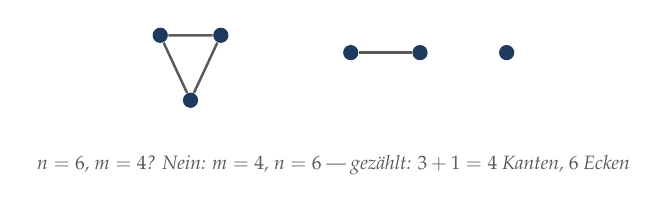
\begin{tikzpicture}[scale=1.1]
\node[knoten] (a) at (-1.6,0.5) {};
\node[knoten] (b) at (-0.9,0.5) {};
\node[knoten] (c) at (-1.25,-0.25) {};
\draw[kante] (a)--(b); \draw[kante] (b)--(c); \draw[kante] (c)--(a);
\node[knoten] (d) at (0.6,0.3) {};
\node[knoten] (e) at (1.4,0.3) {};
\draw[kante] (d)--(e);
\node[knoten] (f) at (2.4,0.3) {};
\node[font=\scriptsize\itshape, color=grau] at (0.4,-1.0) {$n = 6$, $m = 4$? Nein: $m=4$, $n=6$ --- gezählt: $3+1 = 4$ Kanten, $6$ Ecken};
\end{tikzpicture}
\end{center}

Ein sauberes Gegenbeispiel: Nehmen Sie ein Dreieck und eine isolierte Ecke. Dann ist $n = 4$ und $m = 3 = n-1$. Der Graph ist weder zusammenhängend noch kreisfrei --- und damit kein Baum. Die Zahlengleichung stimmt trotzdem.

\begin{center}
\begin{minipage}{0.88\textwidth}
\kursiv{Was hier passiert, sieht man an der Formel $m = n - c$ aus Teil 4: Ein zusätzlicher Kreis erhöht $m$ um eins, eine zusätzliche Komponente senkt es um eins. Beides zusammen hebt sich auf.}
\end{minipage}
\end{center}
\end{warnung}

\section{Blätter}

\begin{merksatz}
\boxtitel{Satz 4.3 --- Jeder Baum mit $n \ge 2$ Ecken hat mindestens zwei Blätter}
\schritt{Beweis --- Schritt 1: einen längsten Weg wählen}
$T$ hat mindestens eine Kante, also gibt es Wege der Länge $\ge 1$. Unter allen Wegen in $T$ wählen wir einen von größtmöglicher Länge:
\[ P = (u_0, u_1, \ldots, u_k), \qquad k \ge 1 . \]
Ein längster existiert, weil ein Weg höchstens $n$ Ecken hat, die Längen also nach oben beschränkt sind.

\schritt{Schritt 2 --- Behauptung: $u_0$ ist ein Blatt}
Angenommen nicht, also $\deg(u_0) \ge 2$. Dann hat $u_0$ außer $u_1$ noch einen weiteren Nachbarn $w$ mit $w \neq u_1$.

\schritt{Schritt 3 --- Fall A: $w$ liegt nicht auf $P$}
Dann ist
\[ (w, u_0, u_1, \ldots, u_k) \]
ein Weg --- alle Ecken sind verschieden, denn $w$ kam auf $P$ nicht vor. Seine Länge ist $k+1 > k$, im Widerspruch zur Wahl von $P$ als längstem Weg.

\schritt{Schritt 4 --- Fall B: $w$ liegt auf $P$}
Dann ist $w = u_j$ für ein $j$. Wegen $w \neq u_1$ und $w \neq u_0$ ist $j \ge 2$. Betrachten wir
\[ (u_0, u_1, \ldots, u_j, u_0) . \]
Das ist ein geschlossener Kantenzug: Die Schritte $u_0 \to u_1 \to \cdots \to u_j$ stammen aus $P$, und der letzte Schritt $u_j \to u_0$ benutzt die Kante $\{u_0, w\} = \{u_0, u_j\}$.

Seine Länge ist $j + 1 \ge 3$, und die Ecken $u_0, \ldots, u_j$ sind paarweise verschieden. Es ist also ein Kreis --- im Widerspruch zur Kreisfreiheit von $T$.

\schritt{Schritt 5 --- Schluss}
Beide Fälle sind unmöglich, also ist $\deg(u_0) = 1$. Dasselbe Argument, angewandt auf das andere Ende, zeigt $\deg(u_k) = 1$. Wegen $k \ge 1$ ist $u_0 \neq u_k$: zwei verschiedene Blätter. $\blacksquare$
\end{merksatz}

\begin{merksatz}
\boxtitel{Folgerung 4.4 --- die mittlere Gradzahl}
In einem Baum mit $n \ge 2$ Ecken ist die Summe aller Grade
\[ \sum_{v} \deg(v) = 2m = 2(n-1) = 2n - 2 . \]
Der Durchschnittsgrad ist also
\[ \frac{2n-2}{n} = 2 - \frac{2}{n} \;<\; 2 . \]

\begin{center}
\begin{minipage}{0.88\textwidth}
\kursiv{Bäume sind knapp unterhalb von Durchschnittsgrad $2$. Da jede Ecke mindestens Grad $1$ hat und der Durchschnitt unter $2$ liegt, muss es Ecken vom Grad $1$ geben --- eine zweite, kürzere Begründung für Satz 4.3, die allerdings nur \kursiv{eine} Ecke liefert. Für \kursiv{zwei} Blätter braucht man das Argument mit dem längsten Weg.}
\end{minipage}
\end{center}
\end{merksatz}

\begin{merksatz}
\boxtitel{Satz 4.5 --- Kante hinzufügen, Kante wegnehmen}
Sei $T$ ein Baum.
\begin{center}
\renewcommand{\arraystretch}{1.55}
\begin{tabular}{@{}P{3.0cm}P{5.6cm}@{}}
\toprule
\textbf{Hinzufügen} & Fügt man zu $T$ eine Kante $\{u,v\} \notin E$ hinzu, so entsteht \kursiv{genau ein} Kreis.\\
\textbf{Wegnehmen} & Entfernt man aus $T$ eine Kante, so zerfällt $T$ in genau zwei Komponenten.\\
\bottomrule
\end{tabular}
\end{center}

\schritt{Beweis, Hinzufügen}
Nach (ii) gibt es in $T$ genau einen Weg $P$ von $u$ nach $v$; seine Länge ist $\ge 2$, weil $\{u,v\}$ keine Kante war. Zusammen mit der neuen Kante ergibt $P$ einen Kreis.

Gäbe es einen zweiten Kreis $C'$ durch die neue Kante, so wäre $C'$ ohne diese Kante ein zweiter Weg von $u$ nach $v$ in $T$ --- Widerspruch zu (ii). Und ein Kreis, der die neue Kante \kursiv{nicht} benutzt, läge ganz in $T$ und widerspräche der Kreisfreiheit.

\schritt{Beweis, Wegnehmen}
Das wurde im Beweis von Teil 2 bereits gezeigt: Jede Kante eines Baumes ist eine Brücke, und $T - e$ hat genau zwei Komponenten. $\blacksquare$
\end{merksatz}

\section{Wurzelbäume}

In den Beispielen des ersten Abschnitts --- Organigramm, Diagnosealgorithmus, Dateiverzeichnis --- gibt es eine ausgezeichnete Ecke: die Klinikleitung, die Eingangsfrage, das oberste Verzeichnis. Das ist eine \kursiv{Zusatzstruktur}, die der Baum selbst nicht mitbringt.

\begin{definition}
\boxtitelm{Definition 4.6 --- Wurzelbaum}
Ein \Begriff{Wurzelbaum} ist ein Paar $(T, r)$ aus einem Baum $T$ und einer ausgezeichneten Ecke $r$, der \Begriff{Wurzel}. Für eine Ecke $v \neq r$ sei $P_v$ der eindeutige Weg von $r$ nach $v$. Dann heißt
\begin{itemize}[leftmargin=1.4em, itemsep=3pt]
\item die vorletzte Ecke auf $P_v$ der \Begriff{Vorgänger} von $v$;
\item $v$ ein \Begriff{Nachfolger} seines Vorgängers;
\item die Länge von $P_v$ die \Begriff{Tiefe} von $v$;
\item die größte vorkommende Tiefe die \Begriff{Höhe} von $(T,r)$.
\end{itemize}
\end{definition}

\begin{merksatz}
\boxtitel{Warum das wohldefiniert ist}
Die Definition beruft sich auf \enquote{den eindeutigen Weg}. Dass es ihn gibt und dass er eindeutig ist, ist genau Aussage (ii) aus Satz 4.2 --- eine Eigenschaft, die wir bewiesen haben und nicht voraussetzen müssen.

\begin{center}
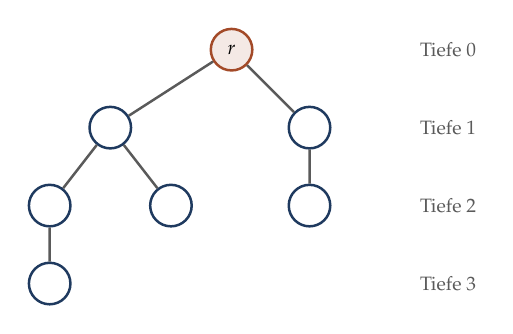
\begin{tikzpicture}[scale=1.1]
\node[knotenr] (r) at (0,1.5) {$r$};
\node[knotenb] (a) at (-1.4,0.6) {};
\node[knotenb] (b) at (0.9,0.6) {};
\node[knotenb] (c) at (-2.1,-0.3) {};
\node[knotenb] (d) at (-0.7,-0.3) {};
\node[knotenb] (e) at (0.9,-0.3) {};
\node[knotenb] (f) at (-2.1,-1.2) {};
\draw[kante] (r)--(a); \draw[kante] (r)--(b);
\draw[kante] (a)--(c); \draw[kante] (a)--(d); \draw[kante] (b)--(e);
\draw[kante] (c)--(f);
\node[font=\scriptsize, color=grau] at (2.5,1.5) {Tiefe $0$};
\node[font=\scriptsize, color=grau] at (2.5,0.6) {Tiefe $1$};
\node[font=\scriptsize, color=grau] at (2.5,-0.3) {Tiefe $2$};
\node[font=\scriptsize, color=grau] at (2.5,-1.2) {Tiefe $3$};
\end{tikzpicture}
\end{center}

Die Höhe dieses Wurzelbaums ist $3$.
\end{merksatz}

\begin{warnung}
\boxtitelr{Wurzel und Höhe sind keine Eigenschaften des Baumes}
Derselbe Baum bekommt je nach Wahl der Wurzel eine andere Höhe.

\begin{center}
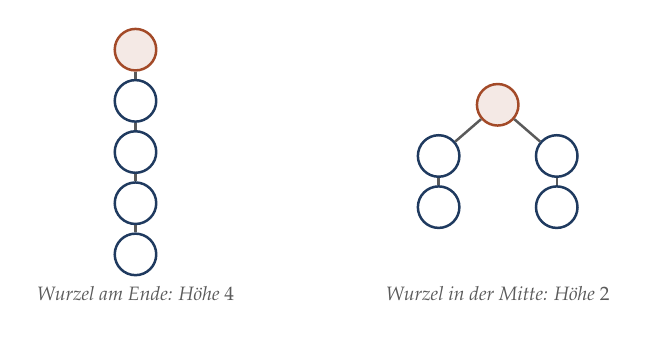
\begin{tikzpicture}[scale=1.0]
\begin{scope}
\node[knotenr] (p0) at (0,1.0) {};
\node[knotenb] (p1) at (0,0.35) {};
\node[knotenb] (p2) at (0,-0.3) {};
\node[knotenb] (p3) at (0,-0.95) {};
\node[knotenb] (p4) at (0,-1.6) {};
\draw[kante] (p0)--(p1);\draw[kante] (p1)--(p2);\draw[kante] (p2)--(p3);\draw[kante] (p3)--(p4);
\node[font=\scriptsize\itshape, color=grau] at (0,-2.1) {Wurzel am Ende: Höhe $4$};
\end{scope}
\begin{scope}[xshift=4.6cm]
\node[knotenr] (q0) at (0,0.3) {};
\node[knotenb] (q1) at (-0.75,-0.35) {};
\node[knotenb] (q2) at (0.75,-0.35) {};
\node[knotenb] (q3) at (-0.75,-1.0) {};
\node[knotenb] (q4) at (0.75,-1.0) {};
\draw[kante] (q0)--(q1);\draw[kante] (q1)--(q3);
\draw[kante] (q0)--(q2);\draw[kante] (q2)--(q4);
\node[font=\scriptsize\itshape, color=grau] at (0,-2.1) {Wurzel in der Mitte: Höhe $2$};
\end{scope}
\end{tikzpicture}
\end{center}

Beide Bilder zeigen denselben Baum $P_5$ --- nur die Wurzel ist verschieden gewählt. Aussagen über \enquote{die Höhe eines Baumes} sind daher unvollständig, solange die Wurzel nicht genannt ist.
\end{warnung}

\section{Übungsaufgaben}

\begin{aufgabe}
\boxtitel{Aufgabe 4.1 --- Ein Baum aus seiner Gradfolge}
Ein Baum hat $12$ Ecken. Genau eine Ecke hat Grad $5$, genau zwei haben Grad $3$, und keine Ecke hat Grad $4$ oder mehr als $5$. Wie viele Blätter hat er, und wie viele Ecken vom Grad $2$?

\loesung
\schritt{Schritt 1 --- Die Unbekannten benennen}
Sei $b$ die Anzahl der Blätter (Grad $1$) und $z$ die Anzahl der Ecken vom Grad $2$. Es gibt keine Ecken vom Grad $0$: Ein Baum mit $n \ge 2$ Ecken ist zusammenhängend, also hat jede Ecke mindestens Grad $1$.

\schritt{Schritt 2 --- Erste Gleichung: die Eckenzahl}
\[ b + z + 2 + 1 = 12 \quad\Longrightarrow\quad b + z = 9 \]
(die $2$ steht für die beiden Ecken vom Grad $3$, die $1$ für die vom Grad $5$).

\schritt{Schritt 3 --- Zweite Gleichung: die Gradsumme}
Nach Folgerung 4.4 ist die Gradsumme $2n - 2 = 2 \cdot 12 - 2 = 22$. Also
\[ 1 \cdot b + 2 \cdot z + 3 \cdot 2 + 5 \cdot 1 = 22 \quad\Longrightarrow\quad b + 2z + 11 = 22 \quad\Longrightarrow\quad b + 2z = 11 . \]

\schritt{Schritt 4 --- Das Gleichungssystem lösen}
Wir ziehen die erste Gleichung von der zweiten ab:
\begin{align*}
(b + 2z) - (b + z) &= 11 - 9\\
z &= 2
\end{align*}
Einsetzen in $b + z = 9$ ergibt $b = 7$.

\schritt{Antwort}
$\mathbf{7}$ Blätter und $\mathbf{2}$ Ecken vom Grad $2$.

\schritt{Probe}
Eckenzahl: $7 + 2 + 2 + 1 = 12$ \checkmark\\
Gradsumme: $7\cdot 1 + 2\cdot 2 + 2\cdot 3 + 1 \cdot 5 = 7 + 4 + 6 + 5 = 22 = 2 \cdot 11 = 2(n-1)$ \checkmark

\schritt{Ein solcher Baum, hingezeichnet}
\begin{center}
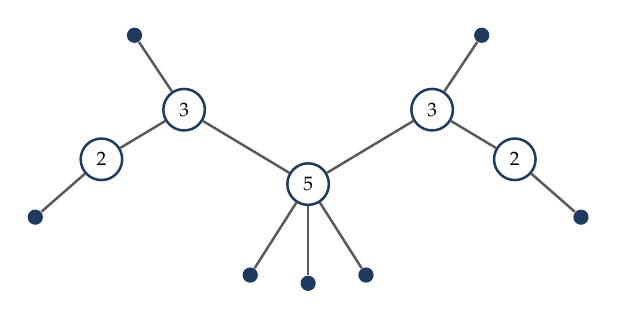
\begin{tikzpicture}[scale=1.05]
\node[knotenb] (z) at (0,0) {$5$};
\node[knotenb] (a) at (-1.5,0.9) {$3$};
\node[knotenb] (b) at (1.5,0.9) {$3$};
\node[knoten] (l1) at (-0.7,-1.1) {};
\node[knoten] (l2) at (0.0,-1.2) {};
\node[knoten] (l3) at (0.7,-1.1) {};
\node[knotenb] (m1) at (-2.5,0.3) {$2$};
\node[knoten] (l4) at (-3.3,-0.4) {};
\node[knoten] (l5) at (-2.1,1.8) {};
\node[knotenb] (m2) at (2.5,0.3) {$2$};
\node[knoten] (l6) at (3.3,-0.4) {};
\node[knoten] (l7) at (2.1,1.8) {};
\draw[kante] (z)--(a); \draw[kante] (z)--(b);
\draw[kante] (z)--(l1); \draw[kante] (z)--(l2); \draw[kante] (z)--(l3);
\draw[kante] (a)--(m1); \draw[kante] (a)--(l5); \draw[kante] (m1)--(l4);
\draw[kante] (b)--(m2); \draw[kante] (b)--(l7); \draw[kante] (m2)--(l6);
\end{tikzpicture}
\end{center}
Nachzählen: $11$ Kanten, $12$ Ecken. \checkmark
\end{aufgabe}

\begin{aufgabe}
\boxtitel{Aufgabe 4.2 --- Eine Ungleichung für Wurzelbäume}
Sei $(T,r)$ ein Wurzelbaum der Höhe $h$, in dem jede Ecke höchstens $k$ Nachfolger hat. Zeigen Sie
\[ n \;\le\; 1 + k + k^2 + \cdots + k^h . \]
Welche Höhe braucht ein solcher Baum mindestens, wenn $n = 1000$ und $k = 2$?

\loesung
\schritt{Schritt 1 --- Nach Tiefen sortieren}
Jede Ecke hat genau eine Tiefe. Sei $a_t$ die Anzahl der Ecken der Tiefe $t$. Dann ist
\[ n = a_0 + a_1 + \cdots + a_h . \]

\schritt{Schritt 2 --- $a_0 = 1$}
Nur die Wurzel hat Tiefe $0$, denn für $v \neq r$ hat der Weg von $r$ nach $v$ Länge $\ge 1$.

\schritt{Schritt 3 --- Der Zusammenhang zwischen den Ebenen}
Jede Ecke $v$ der Tiefe $t+1$ hat einen Vorgänger. Behauptung: Dieser hat Tiefe $t$.

Begründung: Sei $P_v = (r, \ldots, u, v)$ der eindeutige Weg zu $v$, mit Vorgänger $u$. Dann ist $(r, \ldots, u)$ ein Weg von $r$ nach $u$ --- und wegen der Eindeutigkeit \kursiv{der} Weg. Seine Länge ist um $1$ kleiner als die von $P_v$, also hat $u$ die Tiefe $t$.

\schritt{Schritt 4 --- Abschätzen}
Jede Ecke der Tiefe $t+1$ ist Nachfolger einer Ecke der Tiefe $t$, und verschiedene Ecken der Tiefe $t+1$ haben verschiedene\ldots{} nein: Sie können denselben Vorgänger haben. Aber jede Ecke der Tiefe $t$ hat höchstens $k$ Nachfolger. Also
\[ a_{t+1} \;\le\; k \cdot a_t . \]

\schritt{Schritt 5 --- Auflösen}
Aus $a_0 = 1$ folgt der Reihe nach $a_1 \le k$, $a_2 \le k \cdot a_1 \le k^2$, allgemein $a_t \le k^t$. Also
\[ n = \sum_{t=0}^{h} a_t \;\le\; \sum_{t=0}^{h} k^t = 1 + k + \cdots + k^h . \]

\schritt{Schritt 6 --- Der Zahlenwert}
Für $k = 2$ ist die geometrische Summe (Band 3, Kapitel 2)
\[ 1 + 2 + 4 + \cdots + 2^h = 2^{h+1} - 1 . \]
Gefordert ist $2^{h+1} - 1 \ge 1000$, also $2^{h+1} \ge 1001$.

\begin{center}
\renewcommand{\arraystretch}{1.4}
\begin{tabular}{@{}P{1.6cm}P{2.4cm}P{2.6cm}@{}}
\toprule
$h$ & $2^{h+1}-1$ & \textbf{reicht?}\\
\midrule
$8$ & $511$ & nein\\
$\mathbf{9}$ & $\mathbf{1023}$ & \textcolor{gruen}{ja}\\
\bottomrule
\end{tabular}
\end{center}

\schritt{Antwort}
Mindestens Höhe $\mathbf{9}$.

\begin{center}
\begin{minipage}{0.86\textwidth}
\kursiv{Das ist die Rechnung hinter der Bemerkung, dass man in einem Suchbaum mit tausend Einträgen etwa zehn Fragen braucht. Sie ist zugleich der Grund, warum Diagnosealgorithmen mit Ja-Nein-Fragen erstaunlich flach bleiben: Verdoppelt sich die Zahl der Diagnosen, wächst die Höhe nur um eins.}
\end{minipage}
\end{center}
\end{aufgabe}

\begin{aufgabe}
\boxtitel{Aufgabe 4.3 --- Wälder}
Ein Wald hat $n$ Ecken, $m$ Kanten und $c$ Komponenten. Zeigen Sie $m = n - c$, und bestimmen Sie die Anzahl der Komponenten eines Waldes mit $20$ Ecken und $14$ Kanten.

\loesung
\schritt{Schritt 1 --- Die Komponenten sind Bäume}
Jede Komponente eines Waldes ist zusammenhängend (das ist die Definition der Komponente) und kreisfrei (ein Kreis darin wäre einer im Wald). Also ist jede ein Baum.

\schritt{Schritt 2 --- Kantenzahl je Komponente}
Nach Satz 4.2, Aussage (iii), hat die $i$-te Komponente $m_i = n_i - 1$ Kanten.

\schritt{Schritt 3 --- Summieren}
Da jede Kante in genau einer Komponente liegt:
\[ m = \sum_{i=1}^{c} m_i = \sum_{i=1}^{c}(n_i - 1) = n - c . \]

\schritt{Schritt 4 --- Der Zahlenwert}
$14 = 20 - c$, also $c = \mathbf{6}$ Komponenten.

\schritt{Probe an einem Beispiel}
Sechs Bäume mit zusammen $20$ Ecken: etwa fünf Wege $P_3$ ($5 \cdot 3 = 15$ Ecken, $5 \cdot 2 = 10$ Kanten) und ein $P_5$ ($5$ Ecken, $4$ Kanten). Zusammen $20$ Ecken, $14$ Kanten, $6$ Komponenten. \checkmark
\end{aufgabe}

\begin{aufgabe}
\boxtitel{Aufgabe 4.4 --- Zwei Bäume mit gleicher Gradfolge}
Geben Sie zwei nicht isomorphe Bäume mit derselben Gradfolge an. Was folgt daraus für die Invariantenliste aus Kapitel~1?

\loesung
\schritt{Schritt 1 --- Wonach man sucht}
Gesucht sind zwei Bäume mit gleicher Eckenzahl (dann automatisch gleicher Kantenzahl, denn $m = n-1$) und gleicher Gradfolge, die sich dennoch unterscheiden.

\schritt{Schritt 2 --- Die kleinsten Beispiele durchprobieren}
Für $n \le 5$ ist die Gradfolge eines Baumes bereits eindeutig bestimmend --- man kann alle Fälle durchgehen. Bei $n = 6$ wird man fündig.

Wir suchen eine Gradfolge mit Summe $2n-2 = 10$ bei sechs Einträgen. Nehmen wir $(3,2,2,1,1,1)$: Summe $= 3+2+2+1+1+1 = 10$. \checkmark

\schritt{Schritt 3 --- Zwei Bäume dazu}
\begin{center}
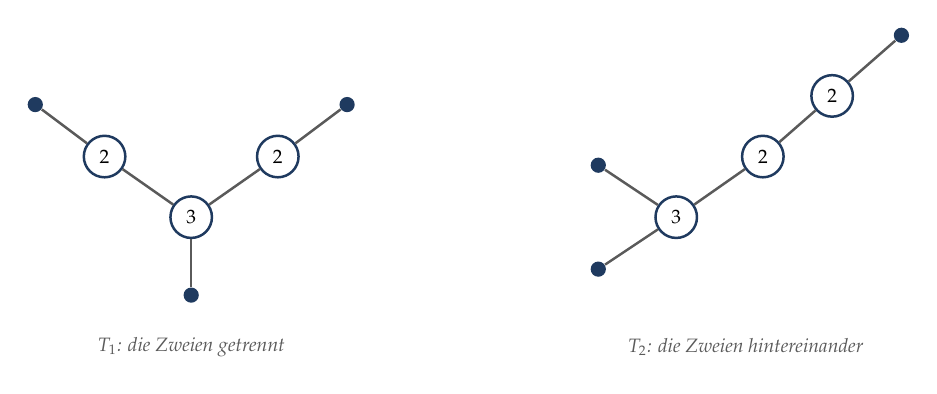
\begin{tikzpicture}[scale=1.1]
\begin{scope}
\node[knotenb] (a) at (0,0) {$3$};
\node[knotenb] (b) at (-1.0,0.7) {$2$};
\node[knotenb] (c) at (1.0,0.7) {$2$};
\node[knoten] (d) at (0,-0.9) {};
\node[knoten] (e) at (-1.8,1.3) {};
\node[knoten] (f) at (1.8,1.3) {};
\draw[kante] (a)--(b); \draw[kante] (a)--(c); \draw[kante] (a)--(d);
\draw[kante] (b)--(e); \draw[kante] (c)--(f);
\node[font=\scriptsize\itshape, color=grau] at (0,-1.5) {$T_1$: die Zweien getrennt};
\end{scope}
\begin{scope}[xshift=5.6cm]
\node[knotenb] (p) at (0,0) {$3$};
\node[knotenb] (q) at (1.0,0.7) {$2$};
\node[knotenb] (s) at (1.8,1.4) {$2$};
\node[knoten] (t) at (2.6,2.1) {};
\node[knoten] (u) at (-0.9,0.6) {};
\node[knoten] (w) at (-0.9,-0.6) {};
\draw[kante] (p)--(q); \draw[kante] (q)--(s); \draw[kante] (s)--(t);
\draw[kante] (p)--(u); \draw[kante] (p)--(w);
\node[font=\scriptsize\itshape, color=grau] at (0.8,-1.5) {$T_2$: die Zweien hintereinander};
\end{scope}
\end{tikzpicture}
\end{center}

\schritt{Schritt 4 --- Nachweis, dass sie nicht isomorph sind}
Wir brauchen eine Invariante, die sie unterscheidet.

\kursiv{Erster Versuch --- die Nachbarn der Ecke vom Grad 3.} In $T_1$ hat die Ecke vom Grad $3$ die Nachbargrade $2, 2, 1$. In $T_2$ hat sie die Nachbargrade $2, 1, 1$. Die Liste der Nachbargrade ist eine Invariante, denn ein Isomorphismus erhält Grade und Nachbarschaften.

Also $T_1 \not\cong T_2$.

\kursiv{Zweiter Versuch zur Kontrolle --- der Durchmesser.} In $T_1$ ist der längste Weg $e - b - a - c - f$, Länge $4$. In $T_2$ ist der längste Weg $u - p - q - s - t$, Länge $4$. Diese Invariante unterscheidet \kursiv{nicht} --- ein gutes Beispiel dafür, dass man mehrere braucht.

\schritt{Schritt 5 --- Was daraus folgt}
Die Gradfolge steht in der Invariantenliste aus Kapitel~1 an dritter Stelle. Sie ist also auch bei Bäumen nicht ausreichend, obwohl Bäume die einfachsten zusammenhängenden Graphen sind.

\begin{center}
\begin{minipage}{0.86\textwidth}
\kursiv{Dass sogar Bäume nicht durch ihre Gradfolge bestimmt sind, macht deutlich, wie weit man von einem praktikablen Isomorphie\-kriterium entfernt ist. Für Bäume gibt es allerdings --- anders als für Graphen allgemein --- ein schnelles Verfahren, das Isomorphie sicher entscheidet; Kapitel~15 nennt es.}
\end{minipage}
\end{center}
\end{aufgabe}

\begin{geschichte}
\boxtitelg{Cayley, die Chemie und die Bäume}
\Person{Arthur Cayley} (1821--1895) führte den Begriff des Baumes 1857 ein, um Differentialoperatoren zu ordnen. Zwanzig Jahre später kam er auf ein ganz anderes Problem zurück: die Zahl der \kursiv{Isomere} gesättigter Kohlenwasserstoffe.

Ein Alkan $\mathrm{C}_k\mathrm{H}_{2k+2}$ lässt sich als Graph auffassen: Kohlenstoffatome sind Ecken vom Grad $4$, Wasserstoffatome Ecken vom Grad $1$. Lässt man die Wasserstoffatome weg, bleibt ein Baum, in dem jede Ecke höchstens vier Nachbarn hat. Die Zahl der Isomere ist die Zahl solcher Bäume bis auf Isomorphie.

Cayley zählte sie 1875 für $k$ bis $13$. Seine Zahlen stimmten mit den damals bekannten Isomeren überein --- ein bemerkenswerter Fall, in dem reine Kombinatorik eine chemische Vorhersage machte.

\begin{center}
{\small
\renewcommand{\arraystretch}{1.4}
\begin{tabular}{@{}P{2.2cm}P{1.6cm}P{1.6cm}P{1.6cm}@{}}
\toprule
\textbf{$k$ Kohlenstoffe} & $4$ & $5$ & $6$\\
\midrule
\textbf{Isomere} & $2$ & $3$ & $5$\\
\bottomrule
\end{tabular}}
\end{center}

\begin{center}
\begin{minipage}{0.9\textwidth}
\kursiv{Die Zählung unbewurzelter Bäume ist schwer, weil man Symmetrien herausrechnen muss. Cayley machte dabei für $k = 13$ einen Fehler; er wurde erst 1931 bemerkt. Das Verfahren, das solche Zählungen zuverlässig macht, stammt von \Person{George Pólya} (1937) und steht in Band 15, Kapitel~9.}
\end{minipage}
\end{center}
\end{geschichte}

\begin{merksatz}
\boxtitel{Was Sie jetzt können}
\begin{center}
\renewcommand{\arraystretch}{1.5}
\begin{tabular}{@{}P{3.0cm}P{5.6cm}@{}}
\toprule
\textbf{Satz 4.2} & Fünf gleichwertige Beschreibungen eines Baumes, im Ringschluss bewiesen\\
\textbf{Satz 4.3} & Jeder Baum mit $n \ge 2$ hat mindestens zwei Blätter\\
\textbf{Satz 4.5} & Kante hinzufügen erzeugt genau einen Kreis; Kante wegnehmen trennt in zwei Teile\\
\textbf{Formel} & $m = n - c$ für jeden Wald\\
\textbf{Wurzelbaum} & Tiefe, Höhe --- und dass beides von der Wurzelwahl abhängt\\
\bottomrule
\end{tabular}
\end{center}

\begin{center}
\begin{minipage}{0.88\textwidth}
\kursiv{Im nächsten Kapitel geht es um Bäume \kursiv{innerhalb} eines Graphen: Wie findet man einen sparsamsten Teilgraphen, der noch alle Ecken verbindet --- und wie viele davon gibt es?}
\end{minipage}
\end{center}
\end{merksatz}

\chapter{Spannbäume und wie man sie zählt}

\section{Das Notrufnetz}

Eine Klinik betreibt an acht Standorten Netzknoten. Zwischen manchen Paaren lässt sich eine Leitung legen; jede kostet eine bestimmte Summe. Verlangt wird: Jeder Standort muss jeden anderen erreichen können --- notfalls über Zwischenknoten. Die Gesamtkosten sollen möglichst klein sein.

\begin{merksatz}
\boxtitel{Was die Aufgabe verlangt --- übersetzt}
\begin{center}
\renewcommand{\arraystretch}{1.5}
\begin{tabular}{@{}P{3.0cm}P{5.6cm}@{}}
\toprule
Standorte & Ecken\\
Mögliche Leitungen & Kanten\\
Kosten & eine Zahl an jeder Kante\\
\enquote{jeder erreicht jeden} & der gewählte Teilgraph ist zusammenhängend und enthält alle Ecken\\
\bottomrule
\end{tabular}
\end{center}

\begin{center}
\begin{minipage}{0.88\textwidth}
\kursiv{Ein Kreis in der Lösung wäre Verschwendung: Nach Satz 2.14 ist jede Kante auf einem Kreis keine Brücke, ließe sich also weglassen, ohne den Zusammenhang zu verlieren. Die Lösung ist somit kreisfrei und zusammenhängend --- ein Baum, der alle Ecken enthält.}
\end{minipage}
\end{center}
\end{merksatz}

\begin{definition}
\boxtitelm{Definition 5.1 --- Spannbaum}
Sei $G = (V,E)$ ein Graph. Ein \Begriff{Spannbaum} von $G$ ist ein Teilgraph $T = (V, E')$ mit $E' \subseteq E$, der \kursiv{alle} Ecken von $G$ enthält und ein Baum ist.
\end{definition}

\begin{merksatz}
\boxtitel{Satz 5.2 --- Jeder zusammenhängende Graph hat einen Spannbaum}
\schritt{Beweis durch Abbauen}
Sei $G$ zusammenhängend. Wir betrachten alle zusammenhängenden Teilgraphen von $G$, die \kursiv{alle} Ecken enthalten. Diese Menge ist nicht leer --- $G$ selbst gehört dazu. Unter ihnen wählen wir einen mit \kursiv{kleinstmöglicher} Kantenzahl und nennen ihn $T$.

\schritt{Behauptung: $T$ ist kreisfrei}
Angenommen, $T$ enthielte einen Kreis, und sei $e$ eine Kante dieses Kreises. Nach Satz 2.14 ist $e$ in $T$ keine Brücke. Also ist $T - e$ noch zusammenhängend, enthält weiterhin alle Ecken (das Weglassen einer Kante entfernt keine Ecke) und hat eine Kante weniger --- im Widerspruch zur Wahl von $T$.

\schritt{Schluss}
$T$ ist zusammenhängend, kreisfrei und enthält alle Ecken. Also ein Spannbaum. $\blacksquare$

\begin{center}
\begin{minipage}{0.88\textwidth}
\kursiv{Nach Satz 4.2 (iii) hat jeder Spannbaum eines Graphen mit $n$ Ecken genau $n-1$ Kanten --- unabhängig davon, welchen man nimmt. Ein Graph mit $m$ Kanten hat also stets $m - n + 1$ Kanten \kursiv{übrig}. Das ist Kirchhoffs zyklomatische Zahl aus Kapitel~3.}
\end{minipage}
\end{center}
\end{merksatz}

\section{Der günstigste Spannbaum}

\begin{definition}
\boxtitelm{Definition 5.3 --- Kantengewichte, minimaler Spannbaum}
Eine \Begriff{Gewichtung} von $G$ ist eine Abbildung $w : E \to \mathbb{R}$, die jeder Kante eine Zahl zuordnet. Das \Begriff{Gewicht} eines Teilgraphen ist die Summe der Gewichte seiner Kanten. Ein \Begriff{minimaler Spannbaum} ist ein Spannbaum kleinstmöglichen Gewichts.
\end{definition}

\begin{merksatz}
\boxtitel{Das Verfahren von Kruskal}
\begin{center}
\renewcommand{\arraystretch}{1.55}
\begin{tabular}{@{}P{1.2cm}P{7.2cm}@{}}
\toprule
1. & Sortiere alle Kanten aufsteigend nach Gewicht.\\
2. & Beginne mit der leeren Kantenmenge $F = \varnothing$.\\
3. & Gehe die Kanten in dieser Reihenfolge durch. Nimm die aktuelle Kante $e$ in $F$ auf, \kursiv{falls} dadurch kein Kreis entsteht; andernfalls überspringe sie.\\
4. & Höre auf, wenn $F$ genau $n-1$ Kanten hat.\\
\bottomrule
\end{tabular}
\end{center}

\begin{center}
\begin{minipage}{0.88\textwidth}
\kursiv{Das Verfahren ist \Begriff{gierig}: Es nimmt in jedem Schritt die billigste noch zulässige Kante und schaut nie zurück. Bei den meisten Optimierungsaufgaben führt so ein Vorgehen in die Irre. Hier nicht --- und der folgende Satz sagt, warum.}
\end{minipage}
\end{center}
\end{merksatz}

\begin{merksatz}
\boxtitel{Satz 5.4 --- Kruskal liefert einen minimalen Spannbaum}
\schritt{Schritt 1 --- Das Ergebnis ist überhaupt ein Spannbaum}
$F$ ist während des ganzen Verfahrens kreisfrei --- das ist die Regel in Zeile 3. Also ist $F$ am Ende ein Wald mit $n-1$ Kanten, und nach der Formel $m = n - c$ aus Aufgabe 4.3 hat er $c = n - (n-1) = 1$ Komponente. Ein zusammenhängender kreisfreier Graph auf allen $n$ Ecken ist ein Spannbaum.

Dass man tatsächlich $n-1$ Kanten zusammenbekommt, sieht man so: Bliebe $F$ mit weniger als $n-1$ Kanten stehen, so hätte $F$ mindestens zwei Komponenten $C_1$, $C_2$. Da $G$ zusammenhängend ist, gibt es in $G$ eine Kante zwischen zwei verschiedenen Komponenten von $F$; diese hätte kein Kreis geschlossen und wäre aufgenommen worden.

\schritt{Schritt 2 --- Die Bezeichnungen für den Kern des Beweises}
Sei $F = \{f_1, f_2, \ldots, f_{n-1}\}$ das Ergebnis, in der Reihenfolge der Aufnahme, also
\[ w(f_1) \le w(f_2) \le \cdots \le w(f_{n-1}) . \]
Sei $T^{*}$ ein minimaler Spannbaum. Zu zeigen: $w(F) \le w(T^{*})$.

\schritt{Schritt 3 --- Den minimalen Spannbaum an $F$ heranschieben}
Wir wählen unter allen minimalen Spannbäumen einen, der mit $F$ \kursiv{möglichst viele} Kanten gemeinsam hat, und nennen ihn wieder $T^{*}$.

Angenommen, $T^{*} \neq F$. Dann gibt es einen kleinsten Index $k$ mit $f_k \notin T^{*}$ --- die ersten $k-1$ Kruskal-Kanten liegen also in $T^{*}$, die $k$-te nicht.

\schritt{Schritt 4 --- Die Kante $f_k$ einfügen}
Nach Satz 4.5 entsteht in $T^{*} + f_k$ genau ein Kreis $C$. Dieser Kreis enthält $f_k$.

\schritt{Schritt 5 --- Eine passende Kante zum Herausnehmen finden}
Behauptung: $C$ enthält eine Kante $g$, die nicht zu $F$ gehört.

Angenommen doch --- alle Kanten von $C$ lägen in $F$. Dann enthielte $F$ einen Kreis, im Widerspruch zur Kreisfreiheit von $F$.

Also gibt es $g \in C$ mit $g \notin F$, und wegen $f_k \in F$ ist $g \neq f_k$.

\schritt{Schritt 6 --- Der Gewichtsvergleich}
Behauptung: $w(f_k) \le w(g)$.

Warum? Betrachten wir den Zeitpunkt, zu dem Kruskal die Kante $f_k$ aufnahm. Zu diesem Zeitpunkt bestand $F$ aus $f_1, \ldots, f_{k-1}$. Hätte $g$ ein kleineres Gewicht als $f_k$, so wäre $g$ vorher an der Reihe gewesen. Kruskal hätte sie geprüft und --- da sie nicht in $F$ landete --- verworfen, weil sie mit $f_1, \ldots, f_{j}$ für ein $j < k$ einen Kreis geschlossen hätte.

Nun liegen aber $f_1, \ldots, f_{k-1}$ alle in $T^{*}$ (Wahl von $k$ in Schritt 3), und $g$ liegt in $T^{*}$ (denn $g \in C \subseteq T^{*} + f_k$ und $g \neq f_k$). Ein Kreis aus $g$ und einigen der $f_1, \ldots, f_{k-1}$ läge damit ganz in $T^{*}$ --- Widerspruch zur Kreisfreiheit von $T^{*}$.

Also war $g$ nicht vor $f_k$ an der Reihe, das heißt $w(g) \ge w(f_k)$.

\schritt{Schritt 7 --- Der Austausch}
Wir setzen
\[ T' = T^{*} + f_k - g . \]
Das ist wieder ein Spannbaum: Die Kante $g$ liegt auf dem Kreis $C$ von $T^{*} + f_k$, ist dort also keine Brücke (Satz 2.14); $T'$ bleibt zusammenhängend, hat $n-1$ Kanten und ist damit nach Satz 4.2 (iii) ein Baum.

Sein Gewicht ist
\[ w(T') = w(T^{*}) + w(f_k) - w(g) \;\le\; w(T^{*}), \]
denn $w(f_k) - w(g) \le 0$ nach Schritt 6.

\schritt{Schritt 8 --- Der Widerspruch}
$T^{*}$ war minimal, also ist $w(T') \ge w(T^{*})$ und damit $w(T') = w(T^{*})$: auch $T'$ ist ein minimaler Spannbaum.

Aber $T'$ hat mit $F$ eine Kante mehr gemeinsam als $T^{*}$ --- es kam $f_k \in F$ hinzu und es fiel $g \notin F$ weg. Das widerspricht der Wahl von $T^{*}$ in Schritt 3.

\schritt{Schritt 9 --- Schluss}
Die Annahme $T^{*} \neq F$ ist falsch. Also ist $F$ selbst ein minimaler Spannbaum. $\blacksquare$
\end{merksatz}

\begin{merksatz}
\boxtitel{Das Notrufnetz, durchgerechnet}
Acht Standorte, mögliche Leitungen mit Kosten in Tausend Euro:

\begin{center}
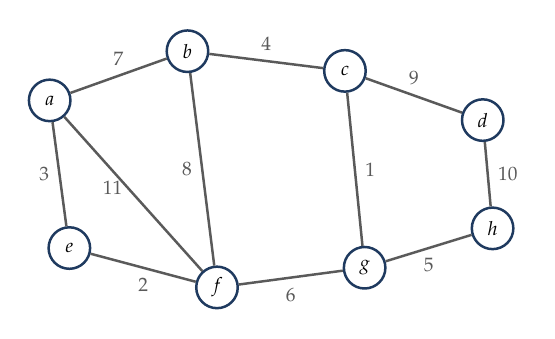
\begin{tikzpicture}[scale=1.25]
\node[knotenb] (a) at (-2.2,1.0) {$a$};
\node[knotenb] (b) at (-0.8,1.5) {$b$};
\node[knotenb] (c) at (0.8,1.3) {$c$};
\node[knotenb] (d) at (2.2,0.8) {$d$};
\node[knotenb] (e) at (-2.0,-0.5) {$e$};
\node[knotenb] (f) at (-0.5,-0.9) {$f$};
\node[knotenb] (g) at (1.0,-0.7) {$g$};
\node[knotenb] (h) at (2.3,-0.3) {$h$};
\draw[kante] (a)--(b) node[midway,above,font=\scriptsize,color=grau] {$7$};
\draw[kante] (b)--(c) node[midway,above,font=\scriptsize,color=grau] {$4$};
\draw[kante] (c)--(d) node[midway,above,font=\scriptsize,color=grau] {$9$};
\draw[kante] (a)--(e) node[midway,left,font=\scriptsize,color=grau] {$3$};
\draw[kante] (e)--(f) node[midway,below,font=\scriptsize,color=grau] {$2$};
\draw[kante] (f)--(g) node[midway,below,font=\scriptsize,color=grau] {$6$};
\draw[kante] (g)--(h) node[midway,below,font=\scriptsize,color=grau] {$5$};
\draw[kante] (b)--(f) node[midway,left,font=\scriptsize,color=grau] {$8$};
\draw[kante] (c)--(g) node[midway,right,font=\scriptsize,color=grau] {$1$};
\draw[kante] (d)--(h) node[midway,right,font=\scriptsize,color=grau] {$10$};
\draw[kante] (a)--(f) node[pos=0.35,below,font=\scriptsize,color=grau] {$11$};
\end{tikzpicture}
\end{center}

\schritt{Schritt 1 --- Sortieren}
\begin{center}
{\small
\renewcommand{\arraystretch}{1.35}
\begin{tabular}{@{}P{1.4cm}P{1.2cm}P{1.4cm}P{1.2cm}P{1.4cm}P{1.2cm}@{}}
\toprule
\textbf{Kante} & \textbf{$w$} & \textbf{Kante} & \textbf{$w$} & \textbf{Kante} & \textbf{$w$}\\
\midrule
$cg$ & $1$ & $bc$ & $4$ & $ab$ & $7$\\
$ef$ & $2$ & $gh$ & $5$ & $bf$ & $8$\\
$ae$ & $3$ & $fg$ & $6$ & $cd$ & $9$\\
& & & & $dh$ & $10$\\
& & & & $af$ & $11$\\
\bottomrule
\end{tabular}}
\end{center}

\schritt{Schritt 2 --- Durchgehen}
\begin{center}
{\small
\renewcommand{\arraystretch}{1.38}
\begin{tabular}{@{}P{1.3cm}P{0.9cm}P{2.2cm}P{3.2cm}@{}}
\toprule
\textbf{Kante} & \textbf{$w$} & \textbf{Aufnehmen?} & \textbf{Begründung}\\
\midrule
$cg$ & $1$ & \textcolor{gruen}{ja} & erste Kante\\
$ef$ & $2$ & \textcolor{gruen}{ja} & kein Kreis\\
$ae$ & $3$ & \textcolor{gruen}{ja} & kein Kreis\\
$bc$ & $4$ & \textcolor{gruen}{ja} & kein Kreis\\
$gh$ & $5$ & \textcolor{gruen}{ja} & kein Kreis\\
$fg$ & $6$ & \textcolor{gruen}{ja} & verbindet $\{a,e,f\}$ mit $\{b,c,g,h\}$\\
$ab$ & $7$ & \textcolor{akzent}{nein} & Kreis $a\!-\!b\!-\!c\!-\!g\!-\!f\!-\!e\!-\!a$\\
$bf$ & $8$ & \textcolor{akzent}{nein} & Kreis $b\!-\!f\!-\!g\!-\!c\!-\!b$\\
$cd$ & $9$ & \textcolor{gruen}{ja} & $d$ war noch nicht dabei\\
\bottomrule
\end{tabular}}
\end{center}

Nach der siebten Aufnahme hat $F$ genau $n-1 = 7$ Kanten. Das Verfahren endet; $dh$ und $af$ werden nicht mehr betrachtet.

\schritt{Schritt 3 --- Das Ergebnis}
\[ F = \{cg,\ ef,\ ae,\ bc,\ gh,\ fg,\ cd\}, \qquad w(F) = 1+2+3+4+5+6+9 = 30 . \]

\schritt{Probe}
Sieben Kanten bei acht Ecken. \checkmark\quad Kreisfrei --- jede aufgenommene Kante verband zwei zuvor getrennte Teile. \checkmark\quad Alle acht Ecken kommen vor: $a$ (in $ae$), $b$ ($bc$), $c$ ($cg$), $d$ ($cd$), $e$ ($ef$), $f$ ($fg$), $g$ ($cg$), $h$ ($gh$). \checkmark

\schritt{Gegenprobe}
Die teuerste weggelassene Kante war $af$ mit $11$. Nähme man sie statt $cd$ mit $9$, wäre $d$ unerreichbar --- das Ergebnis wäre kein Spannbaum. Nähme man $ab$ mit $7$ zusätzlich auf und ließe dafür $fg$ mit $6$ weg, so entstünde ein Gewicht von $31 > 30$.
\end{merksatz}

\section{Wie viele Spannbäume hat der vollständige Graph?}

Die Frage lautet: Wie viele Bäume gibt es auf einer festen Ecken\-menge $\{1, \ldots, n\}$?

\begin{warnung}
\boxtitelr{\enquote{Verschieden} heißt hier etwas anderes als in Kapitel 1}
In Kapitel~1 galten zwei Graphen als gleich, wenn sie isomorph waren. Jetzt sind die Ecken \kursiv{beschriftet}, und zwei Bäume gelten als verschieden, sobald ihre Kantenmengen verschieden sind.

\begin{center}
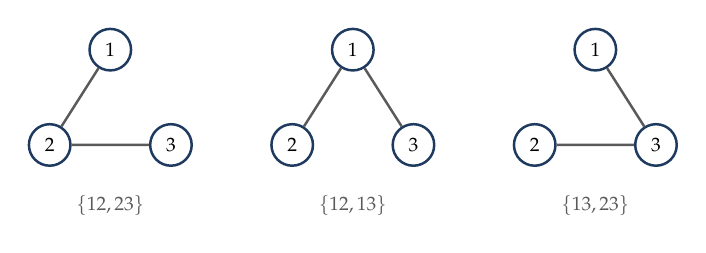
\begin{tikzpicture}[scale=1.1]
\begin{scope}
\node[knotenb] (a1) at (0,0.7) {$1$};
\node[knotenb] (a2) at (-0.7,-0.4) {$2$};
\node[knotenb] (a3) at (0.7,-0.4) {$3$};
\draw[kante] (a1)--(a2); \draw[kante] (a2)--(a3);
\node[font=\scriptsize\itshape, color=grau] at (0,-1.1) {$\{12,23\}$};
\end{scope}
\begin{scope}[xshift=2.8cm]
\node[knotenb] (b1) at (0,0.7) {$1$};
\node[knotenb] (b2) at (-0.7,-0.4) {$2$};
\node[knotenb] (b3) at (0.7,-0.4) {$3$};
\draw[kante] (b1)--(b2); \draw[kante] (b1)--(b3);
\node[font=\scriptsize\itshape, color=grau] at (0,-1.1) {$\{12,13\}$};
\end{scope}
\begin{scope}[xshift=5.6cm]
\node[knotenb] (c1) at (0,0.7) {$1$};
\node[knotenb] (c2) at (-0.7,-0.4) {$2$};
\node[knotenb] (c3) at (0.7,-0.4) {$3$};
\draw[kante] (c1)--(c3); \draw[kante] (c2)--(c3);
\node[font=\scriptsize\itshape, color=grau] at (0,-1.1) {$\{13,23\}$};
\end{scope}
\end{tikzpicture}
\end{center}

Als \kursiv{unbeschriftete} Graphen sind alle drei derselbe Baum $P_3$. Als \kursiv{beschriftete} sind es drei verschiedene. Kapitel~4 zählte die erste Sorte (dort: ein Baum für $n=3$), dieser Abschnitt zählt die zweite.
\end{warnung}

\begin{merksatz}
\boxtitel{Satz 5.5 (Cayley 1889)}
Die Anzahl der Bäume auf der Eckenmenge $\{1, \ldots, n\}$ beträgt für $n \ge 2$ genau
\[ n^{\,n-2} . \]
\end{merksatz}

\begin{merksatz}
\boxtitel{Die Zahlen für kleine $n$}
\begin{center}
\renewcommand{\arraystretch}{1.42}
\begin{tabular}{@{}P{1.2cm}P{1.8cm}P{4.4cm}@{}}
\toprule
$n$ & $n^{n-2}$ & \textbf{Kontrolle}\\
\midrule
$2$ & $2^0 = 1$ & nur die Kante $12$\\
$3$ & $3^1 = 3$ & die drei Bilder oben\\
$4$ & $4^2 = 16$ & $12$ Wege $+$ $4$ Sterne\\
$5$ & $5^3 = 125$ & \\
$6$ & $6^4 = 1296$ & \\
\bottomrule
\end{tabular}
\end{center}

\schritt{Die Kontrolle für $n=4$ nachgerechnet}
Ein Baum auf vier Ecken ist entweder ein Weg $P_4$ oder ein Stern $K_{1,3}$ (Kapitel~4).

\kursiv{Sterne:} Ein Stern ist durch seine Mitte festgelegt. Vier Wahlmöglichkeiten, also $4$ Sterne.

\kursiv{Wege:} Ein Weg auf vier beschrifteten Ecken ist durch die Reihenfolge festgelegt, in der die Ecken durchlaufen werden. Es gibt $4! = 24$ Anordnungen; jeder Weg wird dabei zweimal gezählt (vorwärts und rückwärts). Also $24/2 = 12$ Wege.

Zusammen $12 + 4 = 16 = 4^2$. \checkmark
\end{merksatz}

\subsection*{Der Beweis: das Verfahren von Prüfer}

Der Beweis beruht auf einer Idee von \Person{Heinz Prüfer} (1918): Man ordnet jedem Baum eine Zahlenfolge zu und zeigt, dass diese Zuordnung umkehrbar ist. Da man die Folgen leicht zählen kann, hat man damit auch die Bäume gezählt.

\begin{merksatz}
\boxtitel{Vom Baum zur Folge}
Sei $T$ ein Baum auf $\{1, \ldots, n\}$ mit $n \ge 2$.

\begin{center}
\renewcommand{\arraystretch}{1.55}
\begin{tabular}{@{}P{1.2cm}P{7.2cm}@{}}
\toprule
1. & Suche unter allen Blättern das mit der \kursiv{kleinsten} Beschriftung.\\
2. & Notiere seinen (einzigen) Nachbarn.\\
3. & Entferne das Blatt aus dem Baum.\\
4. & Wiederhole, bis nur noch \kursiv{zwei} Ecken übrig sind.\\
\bottomrule
\end{tabular}
\end{center}

Man führt also $n-2$ Schritte aus und erhält eine Folge $(p_1, \ldots, p_{n-2})$ von Zahlen aus $\{1,\ldots,n\}$. Sie heißt der \Begriff{Prüfer-Code} von $T$.

\schritt{Warum das immer geht}
Nach Satz 4.3 hat jeder Baum mit mindestens zwei Ecken ein Blatt --- Schritt 1 findet also stets eines. Und das Entfernen eines Blattes aus einem Baum liefert wieder einen Baum: Der Rest bleibt zusammenhängend (kein Weg zwischen anderen Ecken lief über ein Blatt, denn ein Blatt hat nur einen Nachbarn und kann keine Durchgangsecke sein) und kreisfrei (Kanten wurden nur weggenommen).
\end{merksatz}

\begin{merksatz}
\boxtitel{Ein Beispiel, vollständig durchgeführt}
\begin{center}
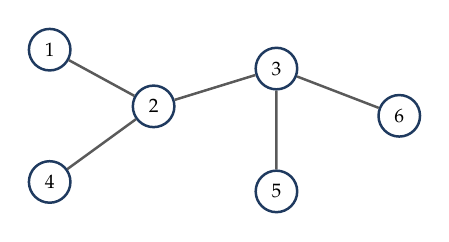
\begin{tikzpicture}[scale=1.2]
\node[knotenb] (1) at (-1.6,0.9) {$1$};
\node[knotenb] (2) at (-0.5,0.3) {$2$};
\node[knotenb] (3) at (0.8,0.7) {$3$};
\node[knotenb] (4) at (-1.6,-0.5) {$4$};
\node[knotenb] (5) at (0.8,-0.6) {$5$};
\node[knotenb] (6) at (2.1,0.2) {$6$};
\draw[kante] (1)--(2); \draw[kante] (4)--(2); \draw[kante] (2)--(3);
\draw[kante] (3)--(5); \draw[kante] (3)--(6);
\end{tikzpicture}
\end{center}

\schritt{Die Durchgänge}
\begin{center}
{\small
\renewcommand{\arraystretch}{1.4}
\begin{tabular}{@{}P{1.2cm}P{2.8cm}P{1.8cm}P{1.6cm}@{}}
\toprule
\textbf{Nr.} & \textbf{Blätter} & \textbf{Kleinstes} & \textbf{Nachbar}\\
\midrule
$1$ & $1, 4, 5, 6$ & $1$ & $\mathbf{2}$\\
$2$ & $4, 5, 6$ & $4$ & $\mathbf{2}$\\
$3$ & $2, 5, 6$ & $2$ & $\mathbf{3}$\\
$4$ & $5, 6$ & $5$ & $\mathbf{3}$\\
\bottomrule
\end{tabular}}
\end{center}

Nach vier Schritten sind noch die Ecken $3$ und $6$ übrig --- das sind zwei, also wird abgebrochen. Der Prüfer-Code lautet
\[ (2,\ 2,\ 3,\ 3) . \]

\schritt{Beobachtung}
Ecke $2$ hatte im Baum Grad $3$ und kommt zweimal im Code vor. Ecke $3$ hatte Grad $3$ und kommt zweimal vor. Die Blätter $1, 4, 5, 6$ kommen gar nicht vor. Das ist kein Zufall:
\[ \deg_T(v) = (\text{Anzahl der Vorkommen von } v \text{ im Code}) + 1 . \]
\end{merksatz}

\begin{merksatz}
\boxtitel{Warum diese Gradformel gilt}
Wir zählen, wie oft die Ecke $v$ im Code auftaucht.

Jedes Mal, wenn ein Nachbar von $v$ als Blatt entfernt wird, wird $v$ notiert. Umgekehrt wird $v$ nur bei solchen Gelegenheiten notiert. Also:
\[ \#\{\text{Vorkommen von } v\} \;=\; \#\{\text{Nachbarn von } v, \text{ die entfernt werden}\} . \]

Nun endet das Verfahren, wenn zwei Ecken übrig sind. Für die Ecke $v$ gibt es zwei Fälle.

\kursiv{Fall 1: $v$ wird selbst irgendwann entfernt.} Zu diesem Zeitpunkt ist $v$ ein Blatt, hat also genau einen verbliebenen Nachbarn. Alle übrigen $\deg_T(v) - 1$ Nachbarn wurden vorher entfernt. Also $\deg_T(v) - 1$ Vorkommen.

\kursiv{Fall 2: $v$ bleibt bis zum Schluss übrig.} Dann ist $v$ eine der beiden Endecken. Von seinen $\deg_T(v)$ Nachbarn ist genau einer ebenfalls übrig --- nämlich der andere Überlebende, denn die beiden Übriggebliebenen bilden einen Baum auf zwei Ecken und sind somit benachbart. Die übrigen $\deg_T(v) - 1$ wurden entfernt. Wieder $\deg_T(v) - 1$ Vorkommen.

In beiden Fällen: Vorkommen $= \deg_T(v) - 1$. $\blacksquare$

\begin{center}
\begin{minipage}{0.88\textwidth}
\kursiv{Insbesondere sind die Blätter genau die Ecken, die im Code \kursiv{nicht} vorkommen. Das ist der Schlüssel zur Umkehrung.}
\end{minipage}
\end{center}
\end{merksatz}

\begin{merksatz}
\boxtitel{Von der Folge zurück zum Baum}
Gegeben sei eine beliebige Folge $(p_1, \ldots, p_{n-2})$ mit Einträgen aus $\{1,\ldots,n\}$.

\begin{center}
\renewcommand{\arraystretch}{1.55}
\begin{tabular}{@{}P{1.2cm}P{7.2cm}@{}}
\toprule
1. & Führe eine Liste $L = \{1,\ldots,n\}$ der noch verfügbaren Ecken.\\
2. & Für $i = 1, \ldots, n-2$: Sei $\ell$ die kleinste Zahl in $L$, die in $(p_i, p_{i+1}, \ldots, p_{n-2})$ \kursiv{nicht} vorkommt. Füge die Kante $\{\ell, p_i\}$ ein und streiche $\ell$ aus $L$.\\
3. & Am Ende sind zwei Zahlen in $L$; verbinde sie durch eine Kante.\\
\bottomrule
\end{tabular}
\end{center}

\schritt{Warum Schritt 2 stets ausführbar ist}
Zu Beginn des $i$-ten Durchgangs enthält $L$ genau $n - i + 1$ Zahlen. Der Restcode $(p_i, \ldots, p_{n-2})$ hat $n-1-i$ Einträge, kann also höchstens $n-1-i$ verschiedene Zahlen enthalten. Wegen
\[ (n-i+1) - (n-1-i) = 2 > 0 \]
bleibt mindestens eine Zahl in $L$ übrig, die nicht im Restcode steht.
\end{merksatz}

\begin{merksatz}
\boxtitel{Die Rückrechnung am Beispiel}
Code $(2,2,3,3)$, also $n = 6$.

\begin{center}
{\small
\renewcommand{\arraystretch}{1.4}
\begin{tabular}{@{}P{0.8cm}P{2.4cm}P{2.0cm}P{1.4cm}P{1.4cm}@{}}
\toprule
$i$ & $L$ & \textbf{Restcode} & $\ell$ & \textbf{Kante}\\
\midrule
$1$ & $1,2,3,4,5,6$ & $2,2,3,3$ & $1$ & $\{1,2\}$\\
$2$ & $2,3,4,5,6$ & $2,3,3$ & $4$ & $\{4,2\}$\\
$3$ & $2,3,5,6$ & $3,3$ & $2$ & $\{2,3\}$\\
$4$ & $3,5,6$ & $3$ & $5$ & $\{5,3\}$\\
\midrule
--- & $3,6$ & --- & --- & $\{3,6\}$\\
\bottomrule
\end{tabular}}
\end{center}

\schritt{Erläuterung der dritten Zeile}
$L = \{2,3,5,6\}$, Restcode $(3,3)$ enthält nur die $3$. Die kleinste Zahl aus $L$, die nicht $3$ ist, lautet $2$. Also Kante $\{2, p_3\} = \{2,3\}$.

\schritt{Ergebnis}
Kanten $\{1,2\}, \{2,4\}, \{2,3\}, \{3,5\}, \{3,6\}$ --- das ist genau der Ausgangsbaum. \checkmark
\end{merksatz}

\begin{merksatz}
\boxtitel{Beweis von Satz 5.5}
\schritt{Schritt 1 --- Die beiden Mengen}
Sei $\mathcal{T}$ die Menge der Bäume auf $\{1,\ldots,n\}$ und $\mathcal{P} = \{1,\ldots,n\}^{n-2}$ die Menge aller Folgen der Länge $n-2$ mit Einträgen aus $\{1,\ldots,n\}$.

\schritt{Schritt 2 --- Die Anzahl der Folgen}
Für jede der $n-2$ Stellen gibt es $n$ Möglichkeiten, unabhängig voneinander. Nach der Produktregel (Band 15, Kapitel 1) ist
\[ |\mathcal{P}| = \underbrace{n \cdot n \cdots n}_{n-2 \text{ Faktoren}} = n^{\,n-2} . \]

\schritt{Schritt 3 --- Die beiden Zuordnungen}
Das erste Verfahren liefert eine Abbildung $\Phi : \mathcal{T} \to \mathcal{P}$, das zweite eine Abbildung $\Psi : \mathcal{P} \to \mathcal{T}$.

Dass $\Psi$ tatsächlich in $\mathcal{T}$ landet --- also einen Baum liefert --- sieht man so: Es werden $(n-2) + 1 = n-1$ Kanten erzeugt. Bei jeder Kante $\{\ell, p_i\}$ wird $\ell$ danach aus $L$ gestrichen und kommt in keiner späteren Kante mehr als $\ell$ vor; als $p_j$ kann es ebenfalls nicht mehr vorkommen, denn $\ell$ wurde ja gerade so gewählt, dass es im Restcode fehlt. Jede erzeugte Kante verbindet also eine \kursiv{endgültig ausscheidende} Ecke mit einer noch aktiven. Damit entsteht nie ein Kreis: Ein Kreis bräuchte an jeder Ecke zwei Kanten, aber $\ell$ bekommt genau eine und verschwindet. Ein kreisfreier Graph auf $n$ Ecken mit $n-1$ Kanten ist nach Satz 4.2 (iv) ein Baum.

\schritt{Schritt 4 --- $\Psi \circ \Phi = \mathrm{id}$}
Sei $T$ ein Baum mit Code $\Phi(T) = (p_1,\ldots,p_{n-2})$. Wir zeigen, dass $\Psi$ im $i$-ten Durchgang dasselbe Blatt wählt, das $\Phi$ im $i$-ten Durchgang entfernt hat.

Betrachte den Zeitpunkt vor dem $i$-ten Durchgang von $\Phi$. Der Restbaum $T_i$ besteht aus den Ecken von $L$. Nach der Gradformel, angewandt auf $T_i$ und den Restcode $(p_i,\ldots,p_{n-2})$, sind die Blätter von $T_i$ genau die Ecken von $L$, die im Restcode nicht vorkommen --- mit einer Feinheit: Die Gradformel gilt für den Restcode einschließlich der abschließenden zwei Ecken, und genau das ist die Situation.

$\Phi$ wählt das kleinste Blatt von $T_i$. $\Psi$ wählt die kleinste Zahl aus $L$, die im Restcode fehlt. Nach dem eben Gesagten sind das dieselben Kandidaten, also dieselbe Wahl. Und die eingetragene Kante ist beide Male $\{\ell, p_i\}$.

Induktiv folgt: Alle $n-2$ Kanten stimmen überein, und die Schlusskante verbindet in beiden Fällen die zwei übriggebliebenen Ecken. Also $\Psi(\Phi(T)) = T$.

\schritt{Schritt 5 --- $\Phi \circ \Psi = \mathrm{id}$}
Dasselbe Argument rückwärts gelesen: Wendet man $\Phi$ auf den von $\Psi$ gebauten Baum an, so wird im $i$-ten Schritt dasselbe Blatt $\ell$ erkannt und derselbe Nachbar $p_i$ notiert.

\schritt{Schritt 6 --- Schluss}
$\Phi$ und $\Psi$ sind zueinander invers, also ist $\Phi$ eine Bijektion. Zwei Mengen, zwischen denen eine Bijektion besteht, haben gleich viele Elemente:
\[ |\mathcal{T}| = |\mathcal{P}| = n^{\,n-2} . \qquad \blacksquare \]
\end{merksatz}

\begin{merksatz}
\boxtitel{Folgerung 5.6 --- Bäume mit vorgeschriebenen Graden}
Die Anzahl der Bäume auf $\{1,\ldots,n\}$, in denen die Ecke $i$ den Grad $d_i$ hat, beträgt
\[ \binom{n-2}{d_1 - 1,\ d_2 - 1,\ \ldots,\ d_n - 1} = \frac{(n-2)!}{(d_1-1)!\,(d_2-1)!\cdots(d_n-1)!} . \]

\schritt{Warum}
Nach der Gradformel ist ein Baum mit diesen Graden dasselbe wie ein Code, in dem die Zahl $i$ genau $d_i - 1$ Mal vorkommt. Die Anzahl solcher Folgen ist der Multinomialkoeffizient aus Band 15, Kapitel~2.

\schritt{Probe}
Für $n=4$ und die Gradfolge $d = (3,1,1,1)$ --- also den Stern mit Mitte $1$ --- ergibt sich
\[ \frac{2!}{2!\,0!\,0!\,0!} = 1 . \]
Es gibt genau einen solchen Baum. \checkmark
\end{merksatz}

\section{Der Matrix-Baum-Satz}

Cayleys Formel zählt die Spannbäume des \kursiv{vollständigen} Graphen. Für beliebige Graphen gibt es eine Formel, die noch überraschender ist: Sie führt die Zählung auf eine Determinante zurück.

\begin{definition}
\boxtitelm{Definition 5.7 --- Laplace-Matrix}
Sei $G$ ein Graph mit Adjazenzmatrix $A$ und sei $D$ die Diagonalmatrix mit den Graden auf der Diagonalen, also $d_{ii} = \deg(v_i)$ und $d_{ij} = 0$ für $i \neq j$. Dann heißt
\[ L = D - A \]
die \Begriff{Laplace-Matrix} von $G$.
\end{definition}

\begin{merksatz}
\boxtitel{Wie $L$ aussieht}
\[ \ell_{ij} = \begin{cases}
\deg(v_i), & i = j,\\
-1, & i \neq j \text{ und } \{v_i,v_j\} \in E,\\
0, & \text{sonst.}
\end{cases} \]

\schritt{Die auffälligste Eigenschaft}
Jede Zeilensumme ist $0$. Denn in Zeile $i$ steht einmal $\deg(v_i)$ und $\deg(v_i)$ Mal die Zahl $-1$:
\[ \deg(v_i) + \deg(v_i)\cdot(-1) = 0 . \]

\begin{center}
\begin{minipage}{0.88\textwidth}
\kursiv{Daraus folgt sofort $\det L = 0$: Addiert man alle Spalten zur ersten, so entsteht eine Nullspalte. Die Determinante der ganzen Matrix ist also nutzlos --- und genau deshalb streicht der folgende Satz eine Zeile und eine Spalte.}
\end{minipage}
\end{center}
\end{merksatz}

\begin{merksatz}
\boxtitel{Satz 5.8 (Kirchhoff 1847, Matrix-Baum-Satz)}
Sei $G$ ein Graph mit $n \ge 2$ Ecken und Laplace-Matrix $L$. Streicht man aus $L$ eine beliebige Zeile $i$ und die zugehörige Spalte $i$, so ist die Determinante der verbleibenden $(n-1)\times(n-1)$-Matrix $L_i$ gleich der Anzahl der Spannbäume von $G$:
\[ \det L_i \;=\; \#\{\text{Spannbäume von } G\} . \]
Das Ergebnis hängt nicht davon ab, welche Zeile gestrichen wird.
\end{merksatz}

\begin{merksatz}
\boxtitel{Ein Beispiel, bevor der Beweis kommt}
Wir nehmen den Kreis $C_4$ mit den Ecken $1,2,3,4$.

\schritt{Die Laplace-Matrix}
Jede Ecke hat Grad $2$; die Kanten sind $12$, $23$, $34$, $41$.
\[ L = \begin{pmatrix}
2 & -1 & 0 & -1\\
-1 & 2 & -1 & 0\\
0 & -1 & 2 & -1\\
-1 & 0 & -1 & 2
\end{pmatrix} \]
Zeilensummen: $2-1+0-1 = 0$ \checkmark

\schritt{Zeile und Spalte 4 streichen}
\[ L_4 = \begin{pmatrix} 2 & -1 & 0\\ -1 & 2 & -1\\ 0 & -1 & 2 \end{pmatrix} \]

\schritt{Determinante ausrechnen --- Entwicklung nach der ersten Zeile}
\[ \det L_4 = 2 \cdot \det\!\begin{pmatrix} 2 & -1\\ -1 & 2\end{pmatrix} - (-1)\cdot \det\!\begin{pmatrix} -1 & -1\\ 0 & 2\end{pmatrix} + 0 \]
\begin{align*}
\det\!\begin{pmatrix} 2 & -1\\ -1 & 2\end{pmatrix} &= 2\cdot 2 - (-1)(-1) = 4 - 1 = 3\\
\det\!\begin{pmatrix} -1 & -1\\ 0 & 2\end{pmatrix} &= (-1)\cdot 2 - (-1)\cdot 0 = -2
\end{align*}
\[ \det L_4 = 2 \cdot 3 + 1 \cdot (-2) = 6 - 2 = 4 \]

\schritt{Probe durch Abzählen}
Ein Spannbaum von $C_4$ entsteht durch Weglassen genau einer Kante ($4$ Kanten, $n-1 = 3$ sollen bleiben). Jede der vier Möglichkeiten liefert einen Weg $P_4$, also einen Baum. Vier Spannbäume. \checkmark

\schritt{Gegenprobe mit einer anderen Zeile}
Streichen wir stattdessen Zeile und Spalte $1$:
\[ L_1 = \begin{pmatrix} 2 & -1 & 0\\ -1 & 2 & -1\\ 0 & -1 & 2\end{pmatrix} \]
Dieselbe Matrix, also wieder $4$. \checkmark
\end{merksatz}

\subsection*{Der Beweis}

\begin{merksatz}
\boxtitel{Schritt 1 --- Kanten eine Richtung geben}
Wir wählen für jede Kante willkürlich eine der beiden Ecken als \enquote{Anfang} und die andere als \enquote{Ende}. Welche, ist gleichgültig --- das Ergebnis wird davon nicht abhängen.

Sei $M$ die $n \times m$-Matrix mit
\[ m_{ie} = \begin{cases}
+1, & \text{falls } v_i \text{ Anfang von } e \text{ ist},\\
-1, & \text{falls } v_i \text{ Ende von } e \text{ ist},\\
0, & \text{falls } v_i \text{ nicht auf } e \text{ liegt.}
\end{cases} \]
Das ist die \Begriff{gerichtete Inzidenzmatrix}. In jeder Spalte steht genau eine $+1$ und genau eine $-1$.
\end{merksatz}

\begin{merksatz}
\boxtitel{Schritt 2 --- Die Schlüsselgleichung $L = M M^{\!\top}$}
Dabei ist $M^{\!\top}$ die \Begriff{Transponierte}: die Matrix, die entsteht, wenn man Zeilen und Spalten vertauscht, also $(M^{\!\top})_{ei} = m_{ie}$.

\schritt{Nachrechnen}
Nach Definition 3.3 ist
\[ (M M^{\!\top})_{ij} = \sum_{e \in E} m_{ie}\, m_{je} . \]

\kursiv{Fall $i = j$.} Dann ist $m_{ie}m_{ie} = m_{ie}^2$. Dieser Wert ist $1$, wenn $v_i$ auf $e$ liegt (denn $(+1)^2 = (-1)^2 = 1$), sonst $0$. Die Summe zählt also die Kanten an $v_i$:
\[ (MM^{\!\top})_{ii} = \deg(v_i) . \]

\kursiv{Fall $i \neq j$.} Der Summand ist nur dann von Null verschieden, wenn \kursiv{beide} Ecken auf $e$ liegen --- also wenn $e = \{v_i, v_j\}$. Da eine Ecke Anfang und die andere Ende ist, ist das Produkt $(+1)\cdot(-1) = -1$. Es gibt höchstens eine solche Kante. Also
\[ (MM^{\!\top})_{ij} = \begin{cases} -1, & \{v_i,v_j\} \in E,\\ 0, & \text{sonst.}\end{cases} \]

Das ist genau die Laplace-Matrix. $\checkmark$

\begin{center}
\begin{minipage}{0.88\textwidth}
\kursiv{Hier zeigt sich, wozu die Vorzeichen gut waren: Ohne sie stünde in der Nebendiagonale $+1$, und die Zeilensummen wären nicht $0$. Die Richtungen sind ein Kunstgriff, der die Buchführung stimmig macht.}
\end{minipage}
\end{center}
\end{merksatz}

\begin{merksatz}
\boxtitel{Schritt 3 --- Der Satz von Cauchy und Binet}
Aus Band 2, Teil IV: Ist $M_i$ eine $(n-1) \times m$-Matrix mit $m \ge n-1$, so gilt
\[ \det\bigl(M_i M_i^{\!\top}\bigr) \;=\; \sum_{S} \bigl(\det M_i[S]\bigr)^2 , \]
wobei über alle Auswahlen $S$ von $n-1$ Spalten summiert wird und $M_i[S]$ die quadratische Matrix aus diesen Spalten bezeichnet.

Streicht man aus $M$ die $i$-te Zeile, so erhält man $M_i$, und aus $L = MM^{\!\top}$ wird
\[ L_i = M_i M_i^{\!\top} . \]
Also
\[ \det L_i = \sum_{S \subseteq E,\ |S| = n-1} \bigl(\det M_i[S]\bigr)^2 . \]

\begin{center}
\begin{minipage}{0.88\textwidth}
\kursiv{Die Summe läuft über alle Auswahlen von $n-1$ Kanten. Es bleibt zu zeigen, dass der Summand genau dann $1$ ist, wenn diese $n-1$ Kanten einen Spannbaum bilden, und sonst $0$. Dann steht rechts genau die Anzahl der Spannbäume.}
\end{minipage}
\end{center}
\end{merksatz}

\begin{merksatz}
\boxtitel{Schritt 4 --- Das Kernlemma}
Sei $S \subseteq E$ mit $|S| = n-1$. Dann gilt
\[ \det M_i[S] = \begin{cases} \pm 1, & \text{falls } S \text{ ein Spannbaum ist},\\ 0, & \text{sonst.}\end{cases} \]

\schritt{Fall A: $S$ ist kein Spannbaum}
Ein Graph auf $n$ Ecken mit $n-1$ Kanten, der kein Spannbaum ist, ist nach Satz 4.2 (iv) nicht kreisfrei --- er enthält also einen Kreis $C$.

Wir behaupten: Die Spalten von $M[S]$, die zu den Kanten von $C$ gehören, sind linear abhängig. Laufen wir den Kreis in einer festen Richtung ab und setzen für jede Kante $\varepsilon_e = +1$, falls wir sie in Richtung Anfang-nach-Ende durchlaufen, sonst $\varepsilon_e = -1$. Dann ist
\[ \sum_{e \in C} \varepsilon_e \cdot (\text{Spalte } e) = 0 . \]
Denn an jeder Ecke des Kreises kommt man einmal an und geht einmal weg; die beiden Beiträge in dieser Zeile sind $+1$ und $-1$ und heben sich auf. An Ecken außerhalb des Kreises stehen ohnehin Nullen.

Diese Abhängigkeit bleibt bestehen, wenn man eine Zeile streicht. Eine quadratische Matrix mit linear abhängigen Spalten hat Determinante $0$ (Band 2, Teil IV).

\schritt{Fall B: $S$ ist ein Spannbaum --- Beweis durch Induktion über $n$}
\textbf{Anfang $n = 2$:} $M_i[S]$ ist eine $1\times 1$-Matrix mit Eintrag $\pm 1$, Determinante $\pm 1$. \checkmark

\textbf{Schritt.} Sei $n \ge 3$. Der Baum $S$ hat nach Satz 4.3 mindestens zwei Blätter; da nur eine Ecke ($v_i$) gestrichen wurde, gibt es ein Blatt $u \neq v_i$. Sei $f$ die einzige Kante an $u$.

In der Matrix $M_i[S]$ steht in der Zeile von $u$ genau ein von Null verschiedener Eintrag, nämlich $\pm 1$ in der Spalte von $f$. Wir entwickeln die Determinante nach dieser Zeile (Band 2, Teil IV):
\[ \det M_i[S] = \pm 1 \cdot \det N, \]
wobei $N$ aus $M_i[S]$ durch Streichen der Zeile von $u$ und der Spalte von $f$ entsteht.

Nun ist $N$ genau die entsprechende Matrix für den Baum $S - u$ im Graphen $G - u$, wieder ohne die Zeile von $v_i$. Der Baum $S-u$ hat $n-1$ Ecken. Nach Induktionsannahme ist $\det N = \pm 1$, also $\det M_i[S] = \pm 1$. $\blacksquare$
\end{merksatz}

\begin{merksatz}
\boxtitel{Schritt 5 --- Zusammensetzen}
Nach dem Kernlemma ist $(\det M_i[S])^2$ gleich $1$ für Spannbäume und $0$ sonst --- das Quadrat beseitigt die Unbestimmtheit des Vorzeichens. Also
\[ \det L_i = \sum_{|S| = n-1} \bigl(\det M_i[S]\bigr)^2 = \#\{\text{Spannbäume}\} . \]
Die rechte Seite hängt offensichtlich nicht von $i$ ab; also auch die linke. $\blacksquare$
\end{merksatz}

\begin{merksatz}
\boxtitel{Cayley als Sonderfall}
Für $G = K_n$ ist $\deg(v) = n-1$ für alle $v$, und alle Nebeneinträge sind $-1$. Also
\[ L = n I - J, \]
wobei $J$ die Matrix aus lauter Einsen ist. Streicht man Zeile und Spalte $n$, so bleibt eine $(n-1)\times(n-1)$-Matrix mit $n-1$ auf der Diagonalen und $-1$ sonst. Ihre Determinante lässt sich mit den Mitteln aus Band 2, Teil IV zu $n^{\,n-2}$ berechnen --- ein zweiter Beweis für Satz 5.5, ganz ohne Kombinatorik.

\begin{center}
\begin{minipage}{0.88\textwidth}
\kursiv{Zwei völlig verschiedene Beweise für dieselbe Formel: einer durch Abzählen von Folgen, einer durch Determinantenrechnung. Der erste erklärt, \kursiv{warum} die Zahl so aussieht; der zweite verallgemeinert auf beliebige Graphen. Beide sind es wert, gekannt zu werden.}
\end{minipage}
\end{center}
\end{merksatz}

\section{Übungsaufgaben}

\begin{aufgabe}
\boxtitel{Aufgabe 5.1 --- Spannbäume abzählen}
Bestimmen Sie die Anzahl der Spannbäume des abgebildeten Graphen auf zwei Wegen: durch Abzählen und mit dem Matrix-Baum-Satz.

\begin{center}
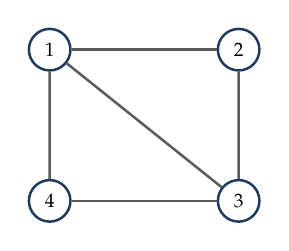
\begin{tikzpicture}[scale=1.2]
\node[knotenb] (1) at (-1.0,0.8) {$1$};
\node[knotenb] (2) at (1.0,0.8) {$2$};
\node[knotenb] (3) at (1.0,-0.8) {$3$};
\node[knotenb] (4) at (-1.0,-0.8) {$4$};
\draw[kante] (1)--(2); \draw[kante] (2)--(3); \draw[kante] (3)--(4);
\draw[kante] (4)--(1); \draw[kante] (1)--(3);
\end{tikzpicture}
\end{center}

\loesung
\schritt{Weg 1 --- Abzählen}
Der Graph hat $n = 4$ Ecken und $m = 5$ Kanten. Ein Spannbaum hat $3$ Kanten, wir lassen also $2$ der $5$ Kanten weg. Es gibt $\binom{5}{2} = 10$ Möglichkeiten.

Wir prüfen jede. Kanten: $a = 12$, $b = 23$, $c = 34$, $d = 41$, $e = 13$.

\begin{center}
{\small
\renewcommand{\arraystretch}{1.32}
\begin{tabular}{@{}P{1.8cm}P{2.4cm}P{3.0cm}@{}}
\toprule
\textbf{Weglassen} & \textbf{Rest} & \textbf{Baum?}\\
\midrule
$a,b$ & $c,d,e$ & \textcolor{akzent}{nein} --- Dreieck $1,3,4$; Ecke $2$ isoliert\\
$a,c$ & $b,d,e$ & \textcolor{gruen}{ja}\\
$a,d$ & $b,c,e$ & \textcolor{gruen}{ja}\\
$a,e$ & $b,c,d$ & \textcolor{gruen}{ja}\\
$b,c$ & $a,d,e$ & \textcolor{gruen}{ja}\\
$b,d$ & $a,c,e$ & \textcolor{gruen}{ja}\\
$b,e$ & $a,c,d$ & \textcolor{gruen}{ja}\\
$c,d$ & $a,b,e$ & \textcolor{akzent}{nein} --- Dreieck $1,2,3$; Ecke $4$ isoliert\\
$c,e$ & $a,b,d$ & \textcolor{gruen}{ja}\\
$d,e$ & $a,b,c$ & \textcolor{gruen}{ja}\\
\bottomrule
\end{tabular}}
\end{center}

Zwei Fälle scheiden aus, es bleiben $\mathbf{8}$ Spannbäume.

\schritt{Weg 2 --- Matrix-Baum-Satz}
Grade: $\deg(1) = 3$ (Nachbarn $2,4,3$), $\deg(2) = 2$, $\deg(3) = 3$, $\deg(4) = 2$.
\[ L = \begin{pmatrix} 3 & -1 & -1 & -1\\ -1 & 2 & -1 & 0\\ -1 & -1 & 3 & -1\\ -1 & 0 & -1 & 2 \end{pmatrix} \]
Zeilensummen alle $0$. \checkmark

Zeile und Spalte $4$ streichen:
\[ L_4 = \begin{pmatrix} 3 & -1 & -1\\ -1 & 2 & -1\\ -1 & -1 & 3 \end{pmatrix} \]

Entwicklung nach der ersten Zeile:
\begin{align*}
\det L_4 &= 3\cdot\det\!\begin{pmatrix}2 & -1\\ -1 & 3\end{pmatrix} - (-1)\cdot\det\!\begin{pmatrix}-1 & -1\\ -1 & 3\end{pmatrix} + (-1)\cdot\det\!\begin{pmatrix}-1 & 2\\ -1 & -1\end{pmatrix}\\[3pt]
&= 3\cdot(6 - 1) + 1\cdot(-3 - 1) - 1\cdot(1 + 2)\\
&= 15 - 4 - 3 = 8
\end{align*}

\schritt{Beide Wege stimmen überein: $\mathbf{8}$ Spannbäume.} \checkmark
\end{aufgabe}

\begin{aufgabe}
\boxtitel{Aufgabe 5.2 --- Prüfer-Code in beide Richtungen}
(a) Bestimmen Sie den Prüfer-Code des Baumes mit den Kanten $\{1,3\}, \{2,3\}, \{3,4\}, \{4,5\}, \{4,6\}, \{6,7\}$.\\
(b) Welcher Baum gehört zum Code $(4,4,1,1,5)$?

\loesung
\schritt{(a) --- Der Baum}
\begin{center}
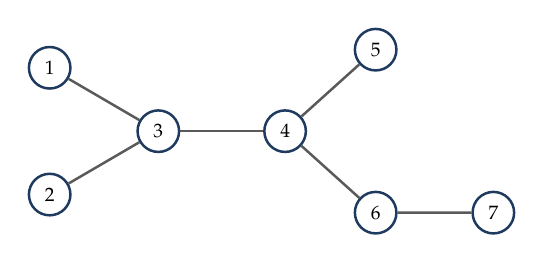
\begin{tikzpicture}[scale=1.15]
\node[knotenb] (1) at (-2.0,0.7) {$1$};
\node[knotenb] (2) at (-2.0,-0.7) {$2$};
\node[knotenb] (3) at (-0.8,0) {$3$};
\node[knotenb] (4) at (0.6,0) {$4$};
\node[knotenb] (5) at (1.6,0.9) {$5$};
\node[knotenb] (6) at (1.6,-0.9) {$6$};
\node[knotenb] (7) at (2.9,-0.9) {$7$};
\draw[kante] (1)--(3);\draw[kante] (2)--(3);\draw[kante] (3)--(4);
\draw[kante] (4)--(5);\draw[kante] (4)--(6);\draw[kante] (6)--(7);
\end{tikzpicture}
\end{center}

$n = 7$, also hat der Code $5$ Einträge.

\begin{center}
{\small
\renewcommand{\arraystretch}{1.4}
\begin{tabular}{@{}P{1.0cm}P{2.6cm}P{1.6cm}P{1.6cm}@{}}
\toprule
\textbf{Nr.} & \textbf{Blätter} & \textbf{Kleinstes} & \textbf{Nachbar}\\
\midrule
$1$ & $1,2,5,7$ & $1$ & $\mathbf{3}$\\
$2$ & $2,5,7$ & $2$ & $\mathbf{3}$\\
$3$ & $3,5,7$ & $3$ & $\mathbf{4}$\\
$4$ & $5,7$ & $5$ & $\mathbf{4}$\\
$5$ & $4,7$ & $4$ & $\mathbf{6}$\\
\bottomrule
\end{tabular}}
\end{center}
Übrig bleiben $6$ und $7$. Code: $(3,3,4,4,6)$.

\schritt{Kontrolle über die Gradformel}
Vorkommen: $3$ zweimal, $4$ zweimal, $6$ einmal. Also $\deg(3) = 3$, $\deg(4) = 3$, $\deg(6) = 2$, alle übrigen $1$.
Im Bild: $\deg(3) = 3$ (Nachbarn $1,2,4$) \checkmark, $\deg(4) = 3$ (Nachbarn $3,5,6$) \checkmark, $\deg(6) = 2$ \checkmark.
Gradsumme $3+3+2+1+1+1+1 = 12 = 2 \cdot 6 = 2(n-1)$ \checkmark

\schritt{(b) --- Rückrechnung für $(4,4,1,1,5)$}
Der Code hat $5$ Einträge, also $n = 7$.

\begin{center}
{\small
\renewcommand{\arraystretch}{1.4}
\begin{tabular}{@{}P{0.8cm}P{2.4cm}P{1.8cm}P{1.2cm}P{1.4cm}@{}}
\toprule
$i$ & $L$ & \textbf{Restcode} & $\ell$ & \textbf{Kante}\\
\midrule
$1$ & $1..7$ & $4,4,1,1,5$ & $2$ & $\{2,4\}$\\
$2$ & $1,3,4,5,6,7$ & $4,1,1,5$ & $3$ & $\{3,4\}$\\
$3$ & $1,4,5,6,7$ & $1,1,5$ & $4$ & $\{4,1\}$\\
$4$ & $1,5,6,7$ & $1,5$ & $6$ & $\{6,1\}$\\
$5$ & $1,5,7$ & $5$ & $1$ & $\{1,5\}$\\
\midrule
--- & $5,7$ & --- & --- & $\{5,7\}$\\
\bottomrule
\end{tabular}}
\end{center}

\schritt{Erläuterung der ersten Zeile}
$L = \{1,\ldots,7\}$, im Restcode kommen $1,4,5$ vor. Die kleinste fehlende Zahl ist $2$.

\schritt{Ergebnis}
Kanten: $\{2,4\}, \{3,4\}, \{1,4\}, \{1,6\}, \{1,5\}, \{5,7\}$.

\begin{center}
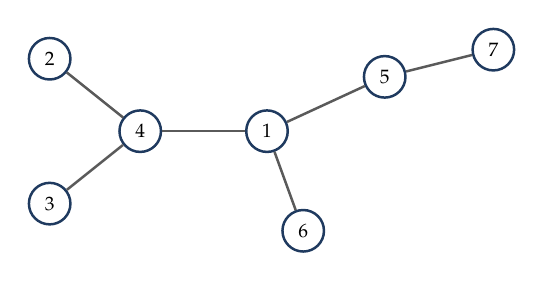
\begin{tikzpicture}[scale=1.15]
\node[knotenb] (4) at (-1.2,0) {$4$};
\node[knotenb] (2) at (-2.2,0.8) {$2$};
\node[knotenb] (3) at (-2.2,-0.8) {$3$};
\node[knotenb] (1) at (0.2,0) {$1$};
\node[knotenb] (6) at (0.6,-1.1) {$6$};
\node[knotenb] (5) at (1.5,0.6) {$5$};
\node[knotenb] (7) at (2.7,0.9) {$7$};
\draw[kante] (4)--(2);\draw[kante] (4)--(3);\draw[kante] (4)--(1);
\draw[kante] (1)--(6);\draw[kante] (1)--(5);\draw[kante] (5)--(7);
\end{tikzpicture}
\end{center}

\schritt{Probe über die Gradformel}
Vorkommen im Code $(4,4,1,1,5)$: $4$ zweimal, $1$ zweimal, $5$ einmal. Erwartete Grade: $\deg(4) = 3$, $\deg(1) = 3$, $\deg(5) = 2$, Rest $1$.
Im Bild: $\deg(4) = 3$ (Nachbarn $2,3,1$) \checkmark, $\deg(1) = 3$ (Nachbarn $4,6,5$) \checkmark, $\deg(5) = 2$ (Nachbarn $1,7$) \checkmark. Sechs Kanten bei sieben Ecken. \checkmark
\end{aufgabe}

\begin{aufgabe}
\boxtitel{Aufgabe 5.3 --- Spannbäume des vollständig bipartiten Graphen}
Der vollständig bipartite Graph $K_{2,3}$ hat wie viele Spannbäume?

\loesung
\schritt{Schritt 1 --- Aufbau}
Ecken $u_1, u_2$ auf der einen Seite, $w_1, w_2, w_3$ auf der anderen; jede Ecke der einen Seite ist mit jeder der anderen verbunden. $n = 5$, $m = 6$.

\schritt{Schritt 2 --- Die Laplace-Matrix}
Grade: $\deg(u_j) = 3$, $\deg(w_k) = 2$. Wir nummerieren $u_1, u_2, w_1, w_2, w_3$.
\[ L = \begin{pmatrix}
3 & 0 & -1 & -1 & -1\\
0 & 3 & -1 & -1 & -1\\
-1 & -1 & 2 & 0 & 0\\
-1 & -1 & 0 & 2 & 0\\
-1 & -1 & 0 & 0 & 2
\end{pmatrix} \]
Zeilensummen: $3+0-1-1-1 = 0$ \checkmark und $-1-1+2+0+0 = 0$ \checkmark

\schritt{Schritt 3 --- Letzte Zeile und Spalte streichen}
\[ L_5 = \begin{pmatrix}
3 & 0 & -1 & -1\\
0 & 3 & -1 & -1\\
-1 & -1 & 2 & 0\\
-1 & -1 & 0 & 2
\end{pmatrix} \]

\schritt{Schritt 4 --- Vereinfachen vor dem Rechnen}
Wir ziehen Zeile 2 von Zeile 1 ab. Das ändert die Determinante nicht (Band 2, Teil IV):
\[ \begin{pmatrix}
3 & -3 & 0 & 0\\
0 & 3 & -1 & -1\\
-1 & -1 & 2 & 0\\
-1 & -1 & 0 & 2
\end{pmatrix} \]
Ebenso Zeile 4 von Zeile 3:
\[ \begin{pmatrix}
3 & -3 & 0 & 0\\
0 & 3 & -1 & -1\\
0 & 0 & 2 & -2\\
-1 & -1 & 0 & 2
\end{pmatrix} \]

\schritt{Schritt 5 --- Entwicklung nach der ersten Spalte}
Einträge der ersten Spalte: $3$ (Zeile 1) und $-1$ (Zeile 4).
\begin{align*}
\det L_5 \;=\;& 3 \cdot \det\!\begin{pmatrix} 3 & -1 & -1\\ 0 & 2 & -2\\ -1 & 0 & 2\end{pmatrix}\\[3pt]
&+\; (-1)\cdot(-1)^{4+1}\det\!\begin{pmatrix} -3 & 0 & 0\\ 3 & -1 & -1\\ 0 & 2 & -2 \end{pmatrix}
\end{align*}

Erste Unterdeterminante, Entwicklung nach der ersten Spalte:
\begin{align*}
&3\cdot\bigl(2\cdot 2 - (-2)\cdot 0\bigr) + (-1)\cdot(-1)^{3+1}\bigl((-1)(-2) - (-1)\cdot 2\bigr)\\
&\qquad = 3\cdot 4 - (2 + 2) = 12 - 4 = 8
\end{align*}

Zweite Unterdeterminante, Entwicklung nach der ersten Zeile:
\[ -3 \cdot \bigl((-1)(-2) - (-1)\cdot 2\bigr) = -3 \cdot (2+2) = -12 \]

Also
\[ \det L_5 = 3 \cdot 8 + (-1)\cdot(-1)\cdot(-12) = 24 - 12 = 12 . \]

\schritt{Antwort}
$K_{2,3}$ hat $\mathbf{12}$ Spannbäume.

\schritt{Probe durch Abzählen}
Ein Spannbaum hat $4$ Kanten von $6$ möglichen, es sind also $2$ wegzulassen: $\binom{6}{2} = 15$ Fälle. Nicht zulässig sind genau die Fälle, in denen eine Ecke $w_k$ beide ihrer Kanten verliert --- dann wäre $w_k$ isoliert. Für jedes der drei $w_k$ gibt es genau einen solchen Fall, und diese drei Fälle sind verschieden. Also $15 - 3 = 12$. \checkmark

\begin{center}
\begin{minipage}{0.86\textwidth}
\kursiv{Allgemein gilt die Formel $r^{s-1} s^{r-1}$ für die Spannbäume von $K_{r,s}$. Für $r=2$, $s=3$: $2^2 \cdot 3^1 = 4 \cdot 3 = 12$. \checkmark}
\end{minipage}
\end{center}
\end{aufgabe}

\begin{geschichte}
\boxtitelg{Borůvka, ein Elektrizitätswerk und drei Wiederentdeckungen}
Das Problem des minimalen Spannbaums wurde 1926 von \Person{Otakar Borůvka} gelöst --- nicht aus mathematischem Interesse, sondern im Auftrag der westmährischen Elektrizitätswerke, die das Stromnetz in Südmähren möglichst günstig aufbauen wollten. Borůvkas Arbeit erschien auf Tschechisch und blieb weitgehend unbeachtet.

\begin{center}
{\small
\renewcommand{\arraystretch}{1.42}
\begin{tabular}{@{}P{2.0cm}P{2.4cm}P{3.8cm}@{}}
\toprule
\textbf{Jahr} & \textbf{Person} & \textbf{Verfahren}\\
\midrule
$1926$ & Borůvka & alle Komponenten gleichzeitig\\
$1930$ & Jarník & von einer Ecke aus wachsen\\
$1956$ & Kruskal & Kanten sortieren\\
$1957$ & Prim & wie Jarník, unabhängig\\
\bottomrule
\end{tabular}}
\end{center}

Das Verfahren aus Zeile 2 heißt heute meist \enquote{Algorithmus von Prim}, obwohl \Person{Vojtěch Jarník} es siebenundzwanzig Jahre früher veröffentlicht hatte --- auf Tschechisch, in einer Antwort auf Borůvkas Arbeit.

\begin{center}
\begin{minipage}{0.9\textwidth}
\kursiv{Die Geschichte ist lehrreich über die Rolle der Sprache in der Wissenschaft. Sie ist auch ein Beispiel dafür, dass dasselbe mathematische Problem viermal unabhängig gelöst werden kann, ohne dass jemand es merkt.}
\end{minipage}
\end{center}
\end{geschichte}

\begin{forschung}
\boxtitelp{Wie schnell findet man einen minimalen Spannbaum?}
Kruskal braucht im Wesentlichen die Zeit zum Sortieren der Kanten, also etwa $m \log m$ Rechenschritte. Das war jahrzehntelang der Stand.

\begin{center}
{\small
\renewcommand{\arraystretch}{1.42}
\begin{tabular}{@{}P{1.6cm}P{2.4cm}P{4.0cm}@{}}
\toprule
\textbf{Jahr} & \textbf{Autoren} & \textbf{Schranke}\\
\midrule
$1956$ & Kruskal & $\Oh(m \log m)$\\
$1975$ & Yao & $\Oh(m \log\log n)$\\
$1995$ & Karger u.\,a. & $\Oh(m)$ mit Zufall\\
$2002$ & Pettie, Ramachandran & optimal --- Schranke unbekannt\\
\bottomrule
\end{tabular}}
\end{center}

Die letzte Zeile beschreibt einen ungewöhnlichen Zustand: Es gibt ein Verfahren, von dem man \kursiv{beweisen} kann, dass es bestmöglich ist --- ohne zu wissen, wie viele Schritte es braucht. Ob ein deterministisches Verfahren mit $\Oh(m)$ Schritten existiert, ist bis heute offen.

\begin{center}
\begin{minipage}{0.9\textwidth}
\kursiv{Der Matrix-Baum-Satz hat inzwischen eine Nebenrolle in der Statistik bekommen: Er liefert die Normierungskonstante für Wahrscheinlichkeitsverteilungen über Spannbäume, wie sie beim Erzeugen zufälliger Netzwerke gebraucht werden.}
\end{minipage}
\end{center}
\end{forschung}

\begin{merksatz}
\boxtitel{Was Sie jetzt können}
\begin{center}
\renewcommand{\arraystretch}{1.5}
\begin{tabular}{@{}P{3.0cm}P{5.6cm}@{}}
\toprule
\textbf{Satz 5.2} & Jeder zusammenhängende Graph hat einen Spannbaum\\
\textbf{Satz 5.4} & Kruskal ist korrekt --- bewiesen durch Austauschargument\\
\textbf{Satz 5.5} & $n^{n-2}$ Bäume auf $n$ beschrifteten Ecken\\
\textbf{Prüfer-Code} & Bijektion zwischen Bäumen und Folgen, in beide Richtungen\\
\textbf{Satz 5.8} & Matrix-Baum-Satz: Spannbäume als Determinante\\
\bottomrule
\end{tabular}
\end{center}

\begin{center}
\begin{minipage}{0.88\textwidth}
\kursiv{Damit ist Teil~II abgeschlossen. Ab Kapitel~6 kehren wir nach Königsberg zurück: Es geht darum, einen Graphen \kursiv{abzulaufen} --- jede Kante genau einmal oder jede Ecke genau einmal.}
\end{minipage}
\end{center}
\end{merksatz}

\part{Durchlaufen}

\chapter{Eulerzüge}

\section{Zurück nach Königsberg}

Die Frage der Bürger lautete: Gibt es einen Spaziergang, der jede der sieben Brücken genau einmal überquert?

Aus Kapitel~1 wissen wir schon, wie der zugehörige Graph aussieht --- und dass er kein Graph im Sinne von Definition 1.1 ist, weil zwischen Insel und Nordufer zwei Brücken verlaufen. Bevor wir die Frage beantworten können, müssen wir den Begriff also erweitern. Das war in Kapitel~1 angekündigt, und hier ist die Stelle.

\begin{definition}
\boxtitelm{Definition 6.1 --- Multigraph}
Ein \Begriff{Multigraph} ist ein Tripel $G = (V, E, \varphi)$ aus
\begin{itemize}[leftmargin=1.4em, itemsep=3pt]
\item einer endlichen, nichtleeren Menge $V$ von Ecken,
\item einer endlichen Menge $E$ von Kanten,
\item einer Abbildung $\varphi$, die jeder Kante $e \in E$ ein Paar $\{u,v\}$ von Ecken zuordnet.
\end{itemize}
Ist $\varphi(e) = \{u,u\}$, so heißt $e$ eine \Begriff{Schlinge}. Zwei verschiedene Kanten mit demselben Bild heißen \Begriff{parallel}.

Der \Begriff{Grad} $\deg(v)$ ist die Anzahl der Kantenenden an $v$; eine Schlinge an $v$ zählt dabei zweimal.
\end{definition}

\begin{merksatz}
\boxtitel{Warum die Kanten jetzt einen eigenen Namen brauchen}
Bei Definition 1.1 \kursiv{war} eine Kante die Menge ihrer beiden Endecken. Zwei Kanten mit denselben Enden wären dann dieselbe Kante --- Parallelen sind unmöglich.

Deshalb trennt Definition 6.1 zwei Dinge, die vorher zusammenfielen: die Kante als eigenständiges Ding (ein Element von $E$) und ihre Lage (das Bild unter $\varphi$). Zwei Brücken zwischen Insel und Nordufer sind zwei verschiedene Elemente von $E$ mit demselben Bild.

\begin{center}
\begin{minipage}{0.88\textwidth}
\kursiv{Das ist ein Muster, das in der Mathematik oft vorkommt: Ein Begriff wird erweitert, indem man eine Identifizierung aufgibt. Alles Bisherige bleibt gültig --- ein Graph nach Definition 1.1 ist ein Multigraph ohne Schlingen und ohne Parallelen.}
\end{minipage}
\end{center}
\end{merksatz}

\begin{merksatz}
\boxtitel{Das Handschlaglemma gilt weiter}
Satz 1.3 bleibt in der Fassung
\[ \sum_{v \in V} \deg(v) = 2\,|E| \]
richtig, und der Beweis ändert sich kaum: Jede Kante hat zwei Enden, jedes Ende liegt an genau einer Ecke.

Die Schlingenregel \enquote{zählt doppelt} ist genau das, was diesen Beweis funktionieren lässt: Eine Schlinge hat zwei Enden, und beide liegen an derselben Ecke. Hätte man Schlingen einfach gezählt, wäre die Formel falsch.
\end{merksatz}

\begin{merksatz}
\boxtitel{Der Königsberger Multigraph}
\begin{center}
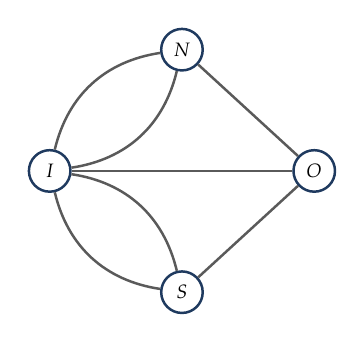
\begin{tikzpicture}[scale=1.4]
\node[knotenb] (N) at (0,1.1) {$N$};
\node[knotenb] (S) at (0,-1.1) {$S$};
\node[knotenb] (I) at (-1.2,0) {$I$};
\node[knotenb] (O) at (1.2,0) {$O$};
\draw[kante] (I) to[bend left=34] (N);
\draw[kante] (I) to[bend right=34] (N);
\draw[kante] (I) to[bend left=34] (S);
\draw[kante] (I) to[bend right=34] (S);
\draw[kante] (I) -- (O);
\draw[kante] (N) -- (O);
\draw[kante] (S) -- (O);
\end{tikzpicture}
\end{center}

\begin{center}
\renewcommand{\arraystretch}{1.45}
\begin{tabular}{@{}P{2.4cm}P{3.6cm}P{1.6cm}@{}}
\toprule
\textbf{Ecke} & \textbf{Kanten} & $\deg$\\
\midrule
Insel $I$ & $2$ nach $N$, $2$ nach $S$, $1$ nach $O$ & $\mathbf{5}$\\
Nordufer $N$ & $2$ nach $I$, $1$ nach $O$ & $\mathbf{3}$\\
Südufer $S$ & $2$ nach $I$, $1$ nach $O$ & $\mathbf{3}$\\
Ostland $O$ & je $1$ nach $I$, $N$, $S$ & $\mathbf{3}$\\
\bottomrule
\end{tabular}
\end{center}

Probe: $5+3+3+3 = 14 = 2 \cdot 7$. \checkmark
\end{merksatz}

\section{Die Begriffe}

\begin{definition}
\boxtitelm{Definition 6.2 --- Eulerzug, Eulerkreis}
Sei $G$ ein Multigraph.
\begin{itemize}[leftmargin=1.4em, itemsep=4pt]
\item Ein \Begriff{Eulerzug} ist ein Kantenzug, der \kursiv{jede Kante von $G$ genau einmal} benutzt.
\item Ein \Begriff{Eulerkreis} ist ein Eulerzug, der an derselben Ecke endet, an der er begann.
\item $G$ heißt \Begriff{eulersch}, wenn er einen Eulerkreis besitzt.
\end{itemize}
\end{definition}

\begin{warnung}
\boxtitelr{Was hier \kursiv{nicht} gefordert wird}
Ein Eulerzug darf Ecken beliebig oft besuchen. Nur die \kursiv{Kanten} dürfen sich nicht wiederholen.

Das ist der Unterschied zum Weg (Definition 2.2), bei dem die Ecken verschieden sein müssen. Und es ist der Unterschied zum Hamiltonkreis des nächsten Kapitels, bei dem umgekehrt jede Ecke genau einmal besucht wird und Kanten übrig bleiben dürfen.

\begin{center}
\renewcommand{\arraystretch}{1.5}
\begin{tabular}{@{}P{2.6cm}P{2.6cm}P{2.6cm}@{}}
\toprule
& \textbf{Jede Kante} & \textbf{Jede Ecke}\\
\midrule
Eulerkreis & \textcolor{gruen}{genau einmal} & beliebig oft\\
Hamiltonkreis & darf fehlen & \textcolor{gruen}{genau einmal}\\
\bottomrule
\end{tabular}
\end{center}

\begin{center}
\begin{minipage}{0.88\textwidth}
\kursiv{Die beiden Begriffe sehen einander zum Verwechseln ähnlich. Sie sind es nicht. Für den einen gibt es ein einfaches, vollständiges Kriterium --- Satz 6.4. Für den anderen kennt niemand eines, und es gibt gute Gründe zu glauben, dass es keines gibt.}
\end{minipage}
\end{center}
\end{warnung}

\section{Die notwendige Bedingung}

\begin{merksatz}
\boxtitel{Satz 6.3 --- Was ein Eulerkreis erzwingt}
Besitzt ein Multigraph $G$ einen Eulerkreis und hat er mindestens eine Kante, so gilt:
\begin{itemize}[leftmargin=1.4em, itemsep=2pt]
\item alle Ecken mit Grad $\ge 1$ liegen in einer einzigen Zusammenhangskomponente,
\item jede Ecke hat geraden Grad.
\end{itemize}
\end{merksatz}

\begin{merksatz}
\boxtitel{Beweis}
\schritt{Erster Teil --- der Zusammenhang}
Der Eulerkreis benutzt jede Kante. Also berührt er jede Ecke, an der eine Kante hängt. Ein Kantenzug verläuft aber innerhalb einer Komponente --- er kann nie von einer Komponente in eine andere springen, weil jeder Schritt eine Kante benutzt. Also liegen alle Ecken mit Grad $\ge 1$ in derselben Komponente.

\schritt{Zweiter Teil --- die Parität}
Sei $v$ eine beliebige Ecke und $Z$ der Eulerkreis. Wir zählen die Kantenenden an $v$ auf zwei Weisen.

\kursiv{Erste Zählung.} Es sind $\deg(v)$ Stück --- das ist die Definition.

\kursiv{Zweite Zählung.} Wir verfolgen $Z$ und zählen, wie oft er die Ecke $v$ berührt.

Jedes Mal, wenn $Z$ die Ecke $v$ als \kursiv{Zwischenecke} durchläuft, kommt er über eine Kante an und geht über eine andere weg. Das verbraucht zwei Kantenenden an $v$.

Bleibt der Start. Der Eulerkreis beginnt an einer Ecke $r$ und endet dort. Ist $v \neq r$, so gibt es keinen weiteren Beitrag: Alle Berührungen sind Durchläufe, also ist $\deg(v)$ das Doppelte der Anzahl der Durchläufe --- gerade.

Ist $v = r$, so kommt zusätzlich das allererste Kantenende (beim Aufbruch) und das allerletzte (bei der Rückkehr) hinzu. Das sind zwei weitere Enden. Also ist auch $\deg(r)$ gerade.

\schritt{Warum jedes Kantenende genau einmal gezählt wird}
Jede Kante an $v$ wird von $Z$ genau einmal benutzt --- das ist die Eulereigenschaft. Bei dieser Benutzung wird genau ein Ende an $v$ verbraucht (oder bei einer Schlinge beide). Es bleibt also kein Ende ungezählt und keines wird doppelt gezählt. $\blacksquare$

\begin{center}
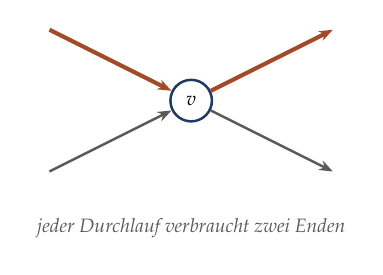
\begin{tikzpicture}[scale=1.2]
\node[knotenb] (v) at (0,0) {$v$};
\draw[kanted, -{Stealth[length=5pt]}] (-1.5,0.75) -- (v);
\draw[kanted, -{Stealth[length=5pt]}] (v) -- (1.5,0.75);
\draw[kante, -{Stealth[length=5pt]}] (-1.5,-0.75) -- (v);
\draw[kante, -{Stealth[length=5pt]}] (v) -- (1.5,-0.75);
\node[font=\scriptsize\itshape, color=grau] at (0,-1.35) {jeder Durchlauf verbraucht zwei Enden};
\end{tikzpicture}
\end{center}
\end{merksatz}

\begin{merksatz}
\boxtitel{Die Antwort für Königsberg}
Der Königsberger Multigraph hat vier Ecken mit den Graden $5, 3, 3, 3$ --- \kursiv{alle vier ungerade}.

Nach Satz 6.3 kann er keinen Eulerkreis besitzen. Und auch keinen offenen Eulerzug, wie Satz 6.5 gleich zeigen wird: Dafür dürfte es höchstens zwei ungerade Ecken geben.

\begin{center}
\begin{minipage}{0.9\textwidth}
\textbf{Der gesuchte Spaziergang existiert nicht.} Nicht, weil man ihn noch nicht gefunden hätte --- sondern weil er nicht existieren kann.
\end{minipage}
\end{center}

\begin{center}
\begin{minipage}{0.88\textwidth}
\kursiv{Beachten Sie, worin die Leistung besteht. Die Bürger konnten beliebig lange probieren, ohne je sicher zu sein, ob sie nur den richtigen Weg noch nicht gefunden hatten. Der Beweis beendet das Probieren. Das ist der Unterschied zwischen \enquote{noch keine Lösung gefunden} und \enquote{es gibt keine}.}
\end{minipage}
\end{center}
\end{merksatz}

\section{Die Bedingung genügt auch}

Satz 6.3 sagt, was ein Eulerkreis erzwingt. Der folgende Satz sagt, dass mehr nicht nötig ist --- und das ist die eigentliche Überraschung.

\begin{merksatz}
\boxtitel{Satz 6.4 (Euler 1736, Hierholzer 1873)}
Ein Multigraph $G$ mit mindestens einer Kante besitzt genau dann einen Eulerkreis, wenn
\begin{itemize}[leftmargin=1.4em, itemsep=2pt]
\item alle Ecken mit Grad $\ge 1$ in einer Komponente liegen und
\item jede Ecke geraden Grad hat.
\end{itemize}
\end{merksatz}

\begin{merksatz}
\boxtitel{Beweis der schwierigen Richtung --- Vorbereitung}
Wir dürfen isolierte Ecken weglassen; sie spielen für Kantenzüge keine Rolle. Sei also $G$ zusammenhängend mit lauter geraden Graden.

\schritt{Hilfssatz --- ein Kreis existiert}
Behauptung: Hat jede Ecke von $G$ geraden Grad und gibt es mindestens eine Kante, so enthält $G$ einen Kreis.

Ist eine Schlinge oder ein Paar paralleler Kanten vorhanden, so hat man bereits einen geschlossenen Kantenzug, der keine Kante wiederholt --- das genügt uns. Andernfalls ist $G$ ein gewöhnlicher Graph, in dem jede Ecke mit Grad $\ge 1$ sogar Grad $\ge 2$ hat (gerade und positiv). Nach dem Beweisverfahren aus Satz 4.3 hat ein kreisfreier Graph mit mindestens einer Kante ein Blatt, also eine Ecke vom Grad $1$ --- Widerspruch. Also gibt es einen Kreis.
\end{merksatz}

\begin{merksatz}
\boxtitel{Beweis --- das Verfahren von Hierholzer}
\schritt{Schritt 1 --- einen ersten geschlossenen Zug bauen}
Wir starten an einer beliebigen Ecke $r$ und laufen los, wobei wir keine Kante zweimal benutzen. Wir laufen so lange, bis es nicht mehr weitergeht.

\kursiv{Behauptung: Wir bleiben in $r$ stecken.} Angenommen, wir bleiben in einer Ecke $v \neq r$ stecken. Bis dahin haben wir $v$ einige Male durchlaufen --- jedes Mal zwei Kantenenden verbraucht --- und sind zuletzt angekommen, ohne weitergehen zu können. Das verbraucht eine ungerade Zahl von Enden an $v$. Da $\deg(v)$ gerade ist, bleibt mindestens ein unbenutztes Ende übrig, über das wir weitergehen könnten. Widerspruch.

Also endet der Zug in $r$: Wir haben einen geschlossenen Kantenzug $Z_1$ ohne Kantenwiederholung.

\schritt{Schritt 2 --- Sind schon alle Kanten dabei?}
Wenn ja, ist $Z_1$ ein Eulerkreis, und wir sind fertig.

Wenn nein, sei $H$ der Multigraph, der aus $G$ durch Entfernen aller Kanten von $Z_1$ entsteht (die Ecken bleiben).

\schritt{Schritt 3 --- $H$ hat wieder lauter gerade Grade}
$Z_1$ ist ein geschlossener Kantenzug. Nach demselben Argument wie im Beweis von Satz 6.3 verbraucht er an jeder Ecke eine \kursiv{gerade} Anzahl von Kantenenden.

Gerade minus gerade ist gerade. Also hat in $H$ jede Ecke geraden Grad.

\schritt{Schritt 4 --- $Z_1$ und der Rest berühren sich}
Behauptung: Es gibt eine Ecke $x$, die auf $Z_1$ liegt und in $H$ noch Grad $\ge 1$ hat.

Angenommen nicht. Dann hätte jede Ecke von $Z_1$ in $H$ den Grad $0$. Da $H$ nach Annahme noch Kanten besitzt, gibt es eine Ecke $y$ mit $\deg_H(y) \ge 1$; sie liegt nicht auf $Z_1$.

$G$ ist aber zusammenhängend, es gibt also einen Weg von $r$ nach $y$ in $G$. Auf diesem Weg gibt es eine erste Ecke, die nicht mehr auf $Z_1$ liegt; die Kante, über die man sie erreicht, geht von einer Ecke von $Z_1$ aus und gehört nicht zu $Z_1$ (denn alle Kanten von $Z_1$ verbinden Ecken von $Z_1$, und diese Kante endet außerhalb). Also liegt sie in $H$ --- und ihre Startecke liegt auf $Z_1$ und hat in $H$ Grad $\ge 1$. Widerspruch.

\schritt{Schritt 5 --- Einen zweiten Zug bauen und einsetzen}
Wir wenden Schritt 1 auf $H$ mit Startecke $x$ an und erhalten einen geschlossenen Kantenzug $Z_2$ durch $x$, der nur Kanten aus $H$ benutzt.

Nun setzen wir zusammen: Wir laufen $Z_1$ ab; sobald wir zum ersten Mal bei $x$ ankommen, schieben wir den ganzen Zug $Z_2$ ein und laufen danach $Z_1$ zu Ende.

\begin{center}
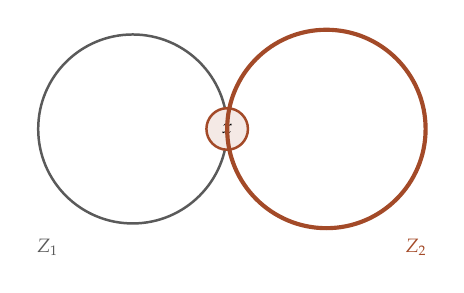
\begin{tikzpicture}[scale=1.2]
\draw[kante] (0,0) circle (1.0);
\node[knotenr] (x) at (1.0,0) {$x$};
\draw[kanted] (2.05,0) circle (1.05);
\node[font=\scriptsize\itshape, color=grau] at (-0.9,-1.25) {$Z_1$};
\node[font=\scriptsize\itshape, color=akzent] at (3.0,-1.25) {$Z_2$};
\end{tikzpicture}
\end{center}

Das Ergebnis ist wieder ein geschlossener Kantenzug ohne Kantenwiederholung --- $Z_1$ und $Z_2$ haben ja keine gemeinsame Kante --- und er ist echt länger als $Z_1$.

\schritt{Schritt 6 --- Warum das Verfahren endet}
Bei jeder Wiederholung von Schritt 2 bis 5 wächst die Zahl der benutzten Kanten um mindestens $1$. Da $G$ nur endlich viele Kanten hat, endet das Verfahren nach höchstens $|E|$ Durchgängen. Es endet aber nur im Fall \enquote{alle Kanten dabei} aus Schritt 2 --- also mit einem Eulerkreis. $\blacksquare$
\end{merksatz}

\begin{merksatz}
\boxtitel{Satz 6.5 --- der offene Eulerzug}
Ein zusammenhängender Multigraph besitzt genau dann einen Eulerzug, der nicht geschlossen ist, wenn er \kursiv{genau zwei} Ecken ungeraden Grades hat. Der Zug beginnt dann in der einen und endet in der anderen.

\schritt{Beweis, Richtung 1}
Sei $Z$ ein offener Eulerzug von $a$ nach $b$ mit $a \neq b$. Dieselbe Zählung wie in Satz 6.3 ergibt: Für $v \notin \{a,b\}$ ist $\deg(v)$ gerade. Bei $a$ kommt das Startende hinzu, bei $b$ das Endende --- je eines, also sind $\deg(a)$ und $\deg(b)$ ungerade.

Nach Satz 1.4 ist die Anzahl ungerader Ecken ohnehin gerade; hier sind es genau zwei.

\schritt{Beweis, Richtung 2 --- der Kunstgriff}
Habe $G$ genau zwei ungerade Ecken $a$ und $b$. Wir fügen eine \kursiv{neue} Kante $e^{*}$ zwischen $a$ und $b$ hinzu und nennen den entstandenen Multigraphen $G^{*}$.

In $G^{*}$ sind $\deg(a)$ und $\deg(b)$ um $1$ gewachsen, also gerade; alle übrigen Grade sind unverändert gerade. $G^{*}$ ist zusammenhängend. Nach Satz 6.4 gibt es einen Eulerkreis $Z^{*}$.

Nun lassen wir aus $Z^{*}$ die Kante $e^{*}$ weg. Da ein Eulerkreis geschlossen ist, darf man ihn an jeder Stelle aufschneiden; wir schneiden ihn so auf, dass $e^{*}$ der letzte Schritt ist. Übrig bleibt ein Kantenzug, der alle Kanten von $G$ genau einmal benutzt und von $b$ nach $a$ läuft. $\blacksquare$

\begin{center}
\begin{minipage}{0.88\textwidth}
\kursiv{Der Kunstgriff --- ein Problem durch \kursiv{Hinzufügen} lösen --- ist typisch. Man macht die Aufgabe scheinbar größer und dafür einfacher, löst sie mit einem bereits bewiesenen Satz und nimmt die Zutat am Schluss wieder heraus.}
\end{minipage}
\end{center}
\end{merksatz}

\section{Wie viele Brücken hätten gefehlt?}

\begin{merksatz}
\boxtitel{Königsberg nachgebessert}
Königsberg hat vier ungerade Ecken. Für einen offenen Eulerzug dürften es zwei sein, für einen Eulerkreis null.

\schritt{Eine zusätzliche Brücke genügt für den offenen Zug}
Baut man eine achte Brücke zwischen zwei der ungeraden Ecken --- etwa zwischen Nordufer und Südufer ---, so werden beide gerade. Übrig bleiben die zwei ungeraden Ecken $I$ und $O$, und nach Satz 6.5 gibt es einen Eulerzug von $I$ nach $O$.

\schritt{Zwei zusätzliche Brücken für den Rundgang}
Für einen Eulerkreis müssen alle vier ungeraden Ecken gerade werden. Zwei Brücken genügen: eine zwischen $N$ und $S$, eine zwischen $I$ und $O$. Weniger geht nicht, denn jede Brücke ändert die Parität von höchstens zwei Ecken.

\schritt{Was tatsächlich geschah}
Von den sieben Brücken wurden im Zweiten Weltkrieg fünf zerstört; zwei wurden nicht wieder aufgebaut, und später kam eine Schnellstraßenbrücke hinzu. Der heutige Graph von Kaliningrad hat genau zwei ungerade Ecken --- ein Eulerzug ist möglich, ein Rundgang nicht.
\end{merksatz}

\begin{merksatz}
\boxtitel{Das Problem des Briefträgers}
Muss ein Briefträger jede Straße mindestens einmal begehen und zum Ausgangspunkt zurückkehren, so sucht er einen kürzesten geschlossenen Kantenzug, der jede Kante mindestens einmal enthält.

\begin{center}
\renewcommand{\arraystretch}{1.5}
\begin{tabular}{@{}P{2.8cm}P{5.8cm}@{}}
\toprule
\textbf{Alle Grade gerade} & Ein Eulerkreis existiert; er ist die Lösung, jede Straße genau einmal.\\
\textbf{$2k$ ungerade Ecken} & Man muss $k$ Wege doppelt gehen --- und zwar so, dass die Gesamtlänge der Doppelungen minimal wird.\\
\bottomrule
\end{tabular}
\end{center}

Die zweite Zeile führt auf eine Aufgabe, die wir erst in Kapitel~11 lösen können: Man muss die ungeraden Ecken paarweise so zuordnen, dass die Summe der Abstände kleinstmöglich ist --- eine \kursiv{Paarung} minimalen Gewichts.

\begin{center}
\begin{minipage}{0.88\textwidth}
\kursiv{Das Problem wurde 1962 von \Person{Mei-Ko Kwan} formuliert und heißt deshalb im Englischen \enquote{Chinese Postman Problem}. Es ist eines der wenigen Rundreiseprobleme, für die ein schnelles Lösungsverfahren bekannt ist --- der scheinbar ähnliche Fall des nächsten Kapitels ist es nicht.}
\end{minipage}
\end{center}
\end{merksatz}

\section{Übungsaufgaben}

\begin{aufgabe}
\boxtitel{Aufgabe 6.1 --- Das Haus vom Nikolaus}
Das bekannte Zeichenspiel verlangt, die abgebildete Figur in einem Zug zu zeichnen, ohne abzusetzen und ohne eine Linie doppelt zu ziehen. Zeigen Sie, dass es geht, und bestimmen Sie alle möglichen Startpunkte.

\begin{center}
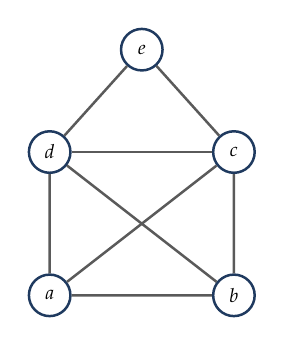
\begin{tikzpicture}[scale=1.3]
\node[knotenb] (a) at (-0.9,-0.9) {$a$};
\node[knotenb] (b) at (0.9,-0.9) {$b$};
\node[knotenb] (c) at (0.9,0.5) {$c$};
\node[knotenb] (d) at (-0.9,0.5) {$d$};
\node[knotenb] (e) at (0,1.5) {$e$};
\draw[kante] (a)--(b);\draw[kante] (b)--(c);\draw[kante] (c)--(d);\draw[kante] (d)--(a);
\draw[kante] (a)--(c);\draw[kante] (b)--(d);\draw[kante] (d)--(e);\draw[kante] (e)--(c);
\end{tikzpicture}
\end{center}

\loesung
\schritt{Schritt 1 --- Grade bestimmen}
\begin{center}
\renewcommand{\arraystretch}{1.42}
\begin{tabular}{@{}P{1.2cm}P{3.4cm}P{1.4cm}P{1.6cm}@{}}
\toprule
\textbf{Ecke} & \textbf{Nachbarn} & $\deg$ & \textbf{Parität}\\
\midrule
$a$ & $b, d, c$ & $3$ & \textcolor{akzent}{ungerade}\\
$b$ & $a, c, d$ & $3$ & \textcolor{akzent}{ungerade}\\
$c$ & $b, d, a, e$ & $4$ & gerade\\
$d$ & $c, a, b, e$ & $4$ & gerade\\
$e$ & $d, c$ & $2$ & gerade\\
\bottomrule
\end{tabular}
\end{center}
Probe: $3+3+4+4+2 = 16 = 2 \cdot 8$. \checkmark

\schritt{Schritt 2 --- Das Kriterium anwenden}
Der Graph ist zusammenhängend und hat \kursiv{genau zwei} Ecken ungeraden Grades, nämlich $a$ und $b$. Nach Satz 6.5 gibt es einen offenen Eulerzug, und er muss in einer der beiden ungeraden Ecken beginnen und in der anderen enden.

\schritt{Schritt 3 --- Antwort auf die Frage nach den Startpunkten}
Die möglichen Startpunkte sind genau $\mathbf{a}$ und $\mathbf{b}$ --- die beiden unteren Ecken. Von $c$, $d$ oder $e$ aus ist es unmöglich.

\schritt{Schritt 4 --- Ein konkreter Zug}
Wir starten in $a$:
\[ a \to b \to c \to a \to d \to b \quad ? \]
Halt: Nach $b$ wären die Kanten $ab$, $bc$, $ca$, $ad$, $db$ verbraucht --- das sind fünf. An $b$ hängen $ab$, $bc$, $bd$, alle drei sind benutzt. Wir stecken fest, obwohl $de$, $ec$, $cd$ übrig sind. Der Zug war zulässig, aber ungeschickt.

Zweiter Versuch:
\[ a \to b \to c \to e \to d \to c \to a \to d \to b \]
Kanten der Reihe nach: $ab$, $bc$, $ce$, $ed$, $dc$, $ca$, $ad$, $db$. Das sind acht verschiedene --- alle. \checkmark\ Der Zug endet in $b$, wie vorhergesagt.

\begin{center}
\begin{minipage}{0.86\textwidth}
\kursiv{Der erste Versuch zeigt etwas Wichtiges: Satz 6.5 garantiert die \kursiv{Existenz}, nicht dass jedes Vorgehen zum Ziel führt. Wer sich verläuft, muss zurück. Das Verfahren von Hierholzer aus dem Beweis vermeidet das systematisch --- es baut Teilkreise und setzt sie ineinander, statt vorwärts zu raten.}
\end{minipage}
\end{center}
\end{aufgabe}

\begin{aufgabe}
\boxtitel{Aufgabe 6.2 --- Wann ist $K_n$ eulersch?}
Für welche $n$ besitzt der vollständige Graph $K_n$ einen Eulerkreis? Für welche einen offenen Eulerzug?

\loesung
\schritt{Schritt 1 --- Die Grade}
In $K_n$ ist jede Ecke mit allen $n-1$ übrigen benachbart, also $\deg(v) = n-1$ für alle $v$.

\schritt{Schritt 2 --- Eulerkreis}
Verlangt sind lauter gerade Grade, also muss $n-1$ gerade sein, also $n$ ungerade. Zusätzlich muss $K_n$ zusammenhängend sein und mindestens eine Kante haben --- das ist für $n \ge 2$ erfüllt.

\textbf{Antwort:} $K_n$ ist eulersch genau für ungerade $n \ge 3$, also $n = 3, 5, 7, 9, \ldots$

\schritt{Schritt 3 --- Offener Eulerzug}
Verlangt sind genau zwei ungerade Ecken. In $K_n$ haben aber \kursiv{alle} $n$ Ecken denselben Grad $n-1$. Sind alle ungerade, so sind es $n$ Stück, und $n = 2$ ist die einzige Möglichkeit.

Für $n = 2$: zwei Ecken vom Grad $1$, eine Kante. Der Zug ist $1 \to 2$. \checkmark

\textbf{Antwort:} Nur $K_2$.

\schritt{Probe an Beispielen}
\begin{center}
\renewcommand{\arraystretch}{1.42}
\begin{tabular}{@{}P{1.2cm}P{1.6cm}P{1.6cm}P{3.0cm}@{}}
\toprule
$n$ & $\deg$ & $m$ & \textbf{Befund}\\
\midrule
$3$ & $2$ & $3$ & Eulerkreis: das Dreieck\\
$4$ & $3$ & $6$ & vier ungerade Ecken --- nichts\\
$5$ & $4$ & $10$ & Eulerkreis mit $10$ Kanten\\
$6$ & $5$ & $15$ & sechs ungerade Ecken --- nichts\\
\bottomrule
\end{tabular}
\end{center}
\end{aufgabe}

\begin{aufgabe}
\boxtitel{Aufgabe 6.3 --- Ein Zerlegungssatz}
Zeigen Sie: Ein Graph, in dem jede Ecke geraden Grad hat, lässt sich in kantendisjunkte Kreise zerlegen --- das heißt, die Kantenmenge lässt sich so in Gruppen aufteilen, dass jede Gruppe ein Kreis ist.

\loesung
\schritt{Schritt 1 --- Induktion über die Kantenzahl}
\textbf{Anfang $m = 0$:} Die leere Zerlegung leistet das Verlangte.

\schritt{Schritt 2 --- Induktionsschritt}
Sei $m \ge 1$ und die Behauptung für alle Graphen mit weniger Kanten und lauter geraden Graden bewiesen.

\schritt{Schritt 3 --- Einen Kreis finden}
Da $m \ge 1$ gibt es eine Ecke mit Grad $\ge 1$, wegen der Parität also mit Grad $\ge 2$. Nach dem Hilfssatz aus dem Beweis von Satz 6.4 enthält $G$ einen Kreis $C$.

\schritt{Schritt 4 --- Ihn herausnehmen}
Sei $G' = G - E(C)$, also $G$ ohne die Kanten von $C$ (die Ecken bleiben).

Ein Kreis berührt jede Ecke entweder gar nicht oder genau zweimal --- er kommt an und geht weg. Also senkt das Entfernen von $C$ jeden Grad um $0$ oder $2$. Gerade minus gerade ist gerade: In $G'$ sind alle Grade weiterhin gerade.

\schritt{Schritt 5 --- Induktionsannahme}
$G'$ hat $m - |C| < m$ Kanten und lauter gerade Grade. Nach Induktionsannahme zerfällt $E(G')$ in kantendisjunkte Kreise.

\schritt{Schritt 6 --- Zusammensetzen}
Fügt man $C$ zu dieser Zerlegung hinzu, so erhält man eine Zerlegung von $E(G)$: Jede Kante liegt entweder in $C$ oder in $G'$, nie in beiden. $\blacksquare$

\schritt{Nachbemerkung --- der Zusammenhang zu Satz 6.4}
Der Satz gilt \kursiv{ohne} Zusammenhangsvoraussetzung. Für einen Eulerkreis braucht man zusätzlich, dass alles in einer Komponente liegt --- erst dann lassen sich die Kreise zu einem einzigen Zug verschmelzen. Das ist genau Schritt 4 des Hierholzer-Beweises.
\end{aufgabe}

\begin{geschichte}
\boxtitelg{Was Euler wirklich bewies --- und was Hierholzer nachtrug}
Eulers Aufsatz von 1736 enthält den notwendigen Teil vollständig: Er zeigt, dass ungerade Grade den Zug verhindern, und beantwortet damit die Königsberger Frage.

Den umgekehrten Teil --- dass gerade Grade genügen --- behauptete er, ohne ihn auszuführen. Er hielt ihn offenbar für offensichtlich. Er ist es nicht: Der Beweis braucht das Verschmelzungsargument aus Schritt 5, und das ist alles andere als selbstverständlich.

Den vollständigen Beweis lieferte \Person{Carl Hierholzer} erst 1873, hundertsiebenunddreißig Jahre später --- und auch das nur beinahe: Hierholzer starb 1871 im Alter von neunundzwanzig Jahren, bevor er die Arbeit niederschreiben konnte. Zwei Kollegen rekonstruierten sie aus seinen Vorträgen und veröffentlichten sie posthum.

\begin{center}
\begin{minipage}{0.9\textwidth}
\kursiv{Der Fall ist ein Musterbeispiel für die Warnung aus dem Vorwort: Ein Bild kann so überzeugend sein, dass selbst Euler den fehlenden Schritt nicht bemerkt. Wer heute schreibt \enquote{die Umkehrung ist klar}, steht in dieser Tradition --- und liegt womöglich ebenso daneben.}
\end{minipage}
\end{center}
\end{geschichte}

\begin{forschung}
\boxtitelp{Eulerzüge in der Sequenzierung des Erbguts}
Beim Zusammensetzen eines Genoms aus kurzen Leseabschnitten wird ein Graph gebaut, in dem die Ecken kurze Zeichenketten fester Länge sind und eine Kante zwei überlappende Ketten verbindet --- der \Begriff{De-Bruijn-Graph}. Die gesuchte Gesamtsequenz entspricht dann einem Eulerzug.

Dass man hier den Euler- und nicht den Hamiltonweg sucht, ist der entscheidende Kunstgriff. Der naheliegende Ansatz --- jede Lesung als Ecke, gesucht ein Weg durch alle Ecken --- führt auf ein Hamiltonproblem und ist praktisch unlösbar. Die Umstellung auf Kanten macht dieselbe Aufgabe schnell lösbar.

\begin{center}
{\small
\renewcommand{\arraystretch}{1.42}
\begin{tabular}{@{}P{3.0cm}P{2.2cm}P{2.8cm}@{}}
\toprule
\textbf{Ansatz} & \textbf{Gesucht} & \textbf{Aufwand}\\
\midrule
Überlappungs\-graph & Hamiltonweg & \textcolor{akzent}{praktisch unlösbar}\\
De-Bruijn-Graph & Eulerzug & \textcolor{gruen}{$\Oh(m)$}\\
\bottomrule
\end{tabular}}
\end{center}

\begin{center}
\begin{minipage}{0.88\textwidth}
\kursiv{Der Ansatz geht auf Pevzner, Tang und Waterman (2001) zurück und ist heute die Grundlage der meisten Zusammensetzungsverfahren. In der Praxis stören Lesefehler und Wiederholungen im Erbgut die Eindeutigkeit erheblich --- ein Genom hat typischerweise sehr viele Eulerzüge, und die Auswahl des richtigen ist der eigentlich schwierige Teil.}
\end{minipage}
\end{center}
\end{forschung}

\begin{merksatz}
\boxtitel{Was Sie jetzt können}
\begin{center}
\renewcommand{\arraystretch}{1.5}
\begin{tabular}{@{}P{3.0cm}P{5.6cm}@{}}
\toprule
\textbf{Multigraph} & Die Erweiterung von Definition 1.1, mit Schlingen und Parallelen\\
\textbf{Satz 6.4} & Eulerkreis $\iff$ zusammenhängend und alle Grade gerade\\
\textbf{Satz 6.5} & Offener Eulerzug $\iff$ genau zwei ungerade Ecken\\
\textbf{Hierholzer} & Ein Verfahren, das den Zug wirklich baut\\
\textbf{Königsberg} & Vier ungerade Ecken --- der Spaziergang existiert nicht\\
\bottomrule
\end{tabular}
\end{center}

\begin{center}
\begin{minipage}{0.88\textwidth}
\kursiv{Das nächste Kapitel stellt dieselbe Frage für Ecken statt Kanten --- und kommt zu einem völlig anderen Ergebnis.}
\end{minipage}
\end{center}
\end{merksatz}

\chapter{Hamiltonkreise}

\section{Dieselbe Frage, anderes Objekt}

Kapitel 6 fragte: Kann man jede \kursiv{Kante} genau einmal durchlaufen? Jetzt fragen wir: Kann man jede \kursiv{Ecke} genau einmal besuchen?

Die beiden Fragen sehen einander so ähnlich, dass man erwartet, die Antworten würden einander ähneln. Sie tun es nicht. Der Unterschied ist einer der lehrreichsten der ganzen Mathematik.

\begin{definition}
\boxtitelm{Definition 7.1 --- Hamiltonweg, Hamiltonkreis}
Sei $G$ ein Graph.
\begin{itemize}[leftmargin=1.4em, itemsep=4pt]
\item Ein \Begriff{Hamiltonweg} ist ein Weg, der jede Ecke von $G$ enthält.
\item Ein \Begriff{Hamiltonkreis} ist ein Kreis, der jede Ecke von $G$ enthält.
\item $G$ heißt \Begriff{hamiltonsch}, wenn er einen Hamiltonkreis besitzt.
\end{itemize}
\end{definition}

\begin{merksatz}
\boxtitel{Ein erster Vergleich}
\begin{center}
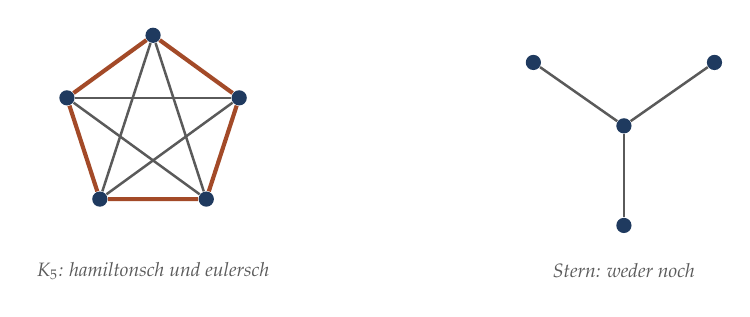
\begin{tikzpicture}[scale=1.15]
\begin{scope}
\foreach \i in {0,...,4} \node[knoten] (a\i) at (90+72*\i:1.0) {};
\foreach \i/\j in {0/1,1/2,2/3,3/4,4/0} \draw[kanted] (a\i) -- (a\j);
\foreach \i/\j in {0/2,1/3,2/4,3/0,4/1} \draw[kante] (a\i) -- (a\j);
\node[font=\scriptsize\itshape, color=grau] at (0,-1.6) {$K_5$: hamiltonsch \kursiv{und} eulersch};
\end{scope}
\begin{scope}[xshift=5.2cm]
\node[knoten] (z) at (0,0) {};
\node[knoten] (p1) at (-1.0,0.7) {};
\node[knoten] (p2) at (1.0,0.7) {};
\node[knoten] (p3) at (0,-1.1) {};
\draw[kante] (z)--(p1); \draw[kante] (z)--(p2); \draw[kante] (z)--(p3);
\node[font=\scriptsize\itshape, color=grau] at (0,-1.6) {Stern: weder noch};
\end{scope}
\end{tikzpicture}
\end{center}

\begin{center}
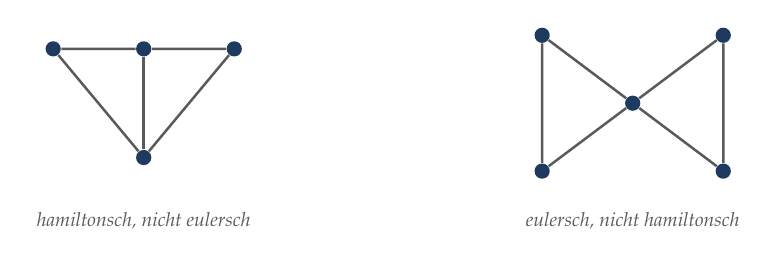
\begin{tikzpicture}[scale=1.15]
\begin{scope}
\node[knoten] (c1) at (-1.0,0.6) {};
\node[knoten] (c2) at (0,0.6) {};
\node[knoten] (c3) at (1.0,0.6) {};
\node[knoten] (c4) at (0,-0.6) {};
\draw[kante] (c1)--(c2); \draw[kante] (c2)--(c3);
\draw[kante] (c1)--(c4); \draw[kante] (c3)--(c4);
\draw[kante] (c2)--(c4);
\node[font=\scriptsize\itshape, color=grau] at (0,-1.3) {hamiltonsch, nicht eulersch};
\end{scope}
\begin{scope}[xshift=5.4cm]
\node[knoten] (m) at (0,0) {};
\node[knoten] (u1) at (-1.0,0.75) {};
\node[knoten] (u2) at (-1.0,-0.75) {};
\node[knoten] (v1) at (1.0,0.75) {};
\node[knoten] (v2) at (1.0,-0.75) {};
\draw[kante] (m)--(u1); \draw[kante] (m)--(u2); \draw[kante] (u1)--(u2);
\draw[kante] (m)--(v1); \draw[kante] (m)--(v2); \draw[kante] (v1)--(v2);
\node[font=\scriptsize\itshape, color=grau] at (0,-1.3) {eulersch, nicht hamiltonsch};
\end{scope}
\end{tikzpicture}
\end{center}

Alle vier Kombinationen kommen vor. Die beiden Begriffe sind also voneinander unabhängig --- keiner folgt aus dem anderen.
\end{merksatz}

\begin{warnung}
\boxtitelr{Der entscheidende Unterschied --- und warum er so groß ist}
\begin{center}
{\small
\renewcommand{\arraystretch}{1.5}
\begin{tabular}{@{}P{2.4cm}P{2.9cm}P{2.9cm}@{}}
\toprule
& \textbf{Eulerkreis} & \textbf{Hamiltonkreis}\\
\midrule
Kriterium & \textcolor{gruen}{Satz 6.4, vollständig} & \textcolor{akzent}{\textbf{keines bekannt}}\\
Prüfaufwand & \textcolor{gruen}{Grade zählen} & \textcolor{akzent}{im Wesentlichen Probieren}\\
Bei $n = 100$ & \textcolor{gruen}{Sekundenbruchteil} & \textcolor{akzent}{unlösbar im Allgemeinen}\\
\bottomrule
\end{tabular}}
\end{center}

Woher der Unterschied? Eine Antwort gibt der Beweis von Satz 6.4. Er funktioniert, weil sich Teilkreise \kursiv{verschmelzen} lassen: Zwei kantendisjunkte geschlossene Züge mit gemeinsamer Ecke ergeben zusammen wieder einen. Man kann also lokal arbeiten und die Stücke zusammensetzen.

Bei Hamiltonkreisen geht das nicht. Zwei Kreise mit gemeinsamer Ecke ergeben keinen Kreis, sondern eine Acht. Es gibt kein Verschmelzungsargument, und deshalb hilft lokales Arbeiten nicht.

\begin{center}
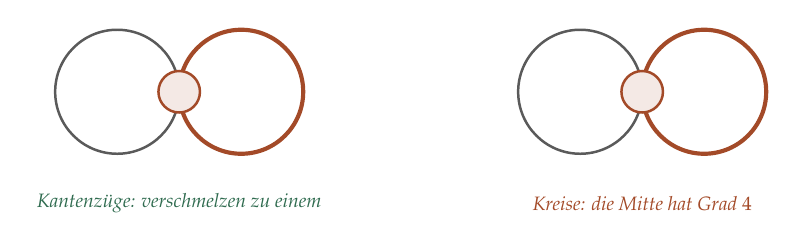
\begin{tikzpicture}[scale=1.05]
\begin{scope}
\draw[kante] (-0.75,0) circle (0.75);
\draw[kanted] (0.75,0) circle (0.75);
\node[knotenr] (x) at (0,0) {};
\node[font=\scriptsize\itshape, color=gruen] at (0,-1.35) {Kantenzüge: verschmelzen zu einem};
\end{scope}
\begin{scope}[xshift=5.6cm]
\draw[kante] (-0.75,0) circle (0.75);
\draw[kanted] (0.75,0) circle (0.75);
\node[knotenr] (y) at (0,0) {};
\node[font=\scriptsize\itshape, color=akzent] at (0,-1.35) {Kreise: die Mitte hat Grad $4$};
\end{scope}
\end{tikzpicture}
\end{center}

\begin{center}
\begin{minipage}{0.88\textwidth}
\kursiv{Dass kein einfaches Kriterium bekannt ist, ist nicht bloß ein Wissenslücke. Kapitel~15 erklärt, warum es aus tiefen Gründen unwahrscheinlich ist, dass eines existiert.}
\end{minipage}
\end{center}
\end{warnung}

\section{Ein Werkzeug zum Widerlegen}

Wenn es kein Kriterium gibt, wie zeigt man dann, dass ein Graph \kursiv{nicht} hamiltonsch ist? Der folgende Satz liefert die meistgenutzte Antwort.

\begin{merksatz}
\boxtitel{Satz 7.2 --- die Komponentenbedingung}
Sei $G$ hamiltonsch. Dann gilt für jede nichtleere Teilmenge $S \subseteq V$:
\[ c(G - S) \;\le\; |S| , \]
wobei $c(\cdot)$ die Anzahl der Zusammenhangskomponenten bezeichnet.
\end{merksatz}

\begin{merksatz}
\boxtitel{Beweis}
\schritt{Schritt 1 --- Den Hamiltonkreis zerschneiden}
Sei $H$ ein Hamiltonkreis von $G$ und $S \subseteq V$ nichtleer mit $|S| = k$.

Wir entfernen die $k$ Ecken von $S$ aus $H$. Ein Kreis, aus dem man $k$ Ecken entfernt, zerfällt in höchstens $k$ Wegstücke.

\schritt{Warum höchstens $k$}
Denken Sie an einen Ring aus Perlen. Nimmt man eine Perle heraus, wird der Ring zu einer Kette --- ein Stück. Nimmt man eine zweite heraus, zerfällt die Kette in zwei Stücke. Jede weitere entfernte Perle erhöht die Stückzahl um höchstens eins.

Genauer: Nach dem Entfernen der ersten Ecke haben wir $1$ Stück. Jede weitere entfernte Ecke liegt in genau einem Stück und teilt dieses in höchstens $2$ Teile --- weniger, wenn sie am Rand liegt. Also nach $k$ Entfernungen höchstens $k$ Stücke.

\begin{center}
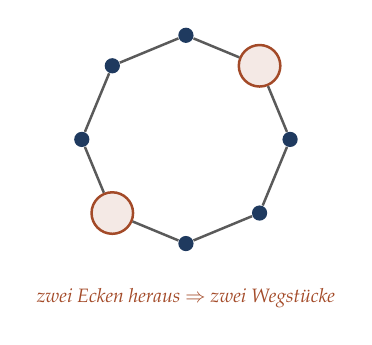
\begin{tikzpicture}[scale=1.15]
\foreach \i in {0,...,7} {
  \pgfmathsetmacro{\ang}{90-45*\i}
  \ifnum\i=1 \node[knotenr] (h\i) at (\ang:1.15) {}; \else
  \ifnum\i=5 \node[knotenr] (h\i) at (\ang:1.15) {}; \else
  \node[knoten] (h\i) at (\ang:1.15) {}; \fi \fi
}
\foreach \i/\j in {0/1,1/2,2/3,3/4,4/5,5/6,6/7,7/0} \draw[kante] (h\i) -- (h\j);
\node[font=\scriptsize\itshape, color=akzent] at (0,-1.75) {zwei Ecken heraus $\Rightarrow$ zwei Wegstücke};
\end{tikzpicture}
\end{center}

\schritt{Schritt 2 --- Von $H$ auf $G$ schließen}
$H$ ist ein Teilgraph von $G$ mit derselben Eckenmenge. Also ist $H - S$ ein Teilgraph von $G - S$ mit derselben Eckenmenge.

Fügt man zu einem Graphen Kanten hinzu, so kann die Komponentenzahl nur sinken oder gleich bleiben --- nie steigen. Denn zwei Ecken, die vorher verbunden waren, bleiben es.

Also
\[ c(G-S) \;\le\; c(H-S) \;\le\; k = |S| . \qquad \blacksquare \]
\end{merksatz}

\begin{merksatz}
\boxtitel{Wie man den Satz benutzt}
Der Satz sagt: \kursiv{Ist} $G$ hamiltonsch, \kursiv{dann} gilt die Ungleichung. Man benutzt ihn in der umgekehrten Richtung: Findet man ein $S$, für das sie verletzt ist, so ist $G$ nicht hamiltonsch.

\begin{center}
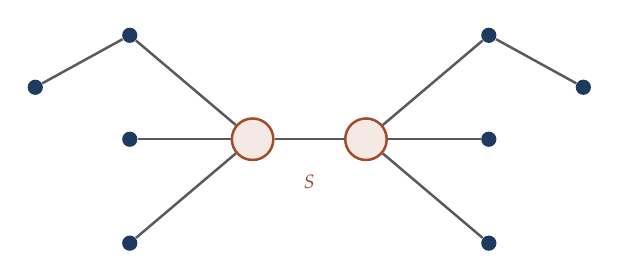
\begin{tikzpicture}[scale=1.2]
\node[knotenr] (m1) at (-0.6,0) {};
\node[knotenr] (m2) at (0.6,0) {};
\foreach \i/\y in {0/1.1, 1/0.0, 2/-1.1} {
  \node[knoten] (l\i) at (-1.9,\y) {};
  \node[knoten] (r\i) at (1.9,\y) {};
}
\node[knoten] (l3) at (-2.9,0.55) {};
\node[knoten] (r3) at (2.9,0.55) {};
\draw[kante] (m1)--(l0);\draw[kante] (m1)--(l1);\draw[kante] (m1)--(l2);
\draw[kante] (m2)--(r0);\draw[kante] (m2)--(r1);\draw[kante] (m2)--(r2);
\draw[kante] (m1)--(m2);
\draw[kante] (l0)--(l3);\draw[kante] (r0)--(r3);
\node[font=\scriptsize, color=akzent] at (0,-0.45) {$S$};
\end{tikzpicture}
\end{center}

\schritt{Beispiel}
Wählt man $S$ als die beiden roten Ecken, so zerfällt der Rest in sechs Teile: links drei (die drei Zweige, von denen einer zwei Ecken hat), rechts drei. Also
\[ c(G-S) = 6 \;>\; 2 = |S| . \]
Der Graph ist nicht hamiltonsch.

\begin{center}
\begin{minipage}{0.88\textwidth}
\kursiv{Als Sonderfall enthält der Satz: Ein hamiltonscher Graph hat keine Schnittecke. Denn für $S = \{v\}$ mit einer Schnittecke $v$ wäre $c(G-v) \ge 2 > 1$. Anschaulich: Ein Rundgang, der zurückkehren muss, kann keinen Engpass nur einmal durchqueren.}
\end{minipage}
\end{center}
\end{merksatz}

\begin{warnung}
\boxtitelr{Die Bedingung ist notwendig, aber nicht hinreichend}
Es gibt Graphen, die die Komponentenbedingung für \kursiv{jedes} $S$ erfüllen und trotzdem keinen Hamiltonkreis haben. Der Petersen-Graph ist so einer --- Abschnitt 7.5.

Das ist kein Mangel dieses Satzes, sondern die Regel: Alle bekannten notwendigen Bedingungen sind unvollständig, und alle bekannten hinreichenden Bedingungen sind zu stark. Dazwischen bleibt eine Lücke, die niemand schließen konnte.
\end{warnung}

\section{Zwei hinreichende Bedingungen}

Wenn schon kein vollständiges Kriterium, dann wenigstens Bedingungen, die den Hamiltonkreis \kursiv{garantieren}. Die berühmteste stammt von Ore; die bekanntere von Dirac folgt daraus.

\begin{merksatz}
\boxtitel{Satz 7.3 (Ore 1960)}
Sei $G$ ein Graph mit $n \ge 3$ Ecken. Gilt für je zwei \kursiv{nicht benachbarte} Ecken $u,v$
\[ \deg(u) + \deg(v) \;\ge\; n , \]
so ist $G$ hamiltonsch.
\end{merksatz}

\begin{merksatz}
\boxtitel{Beweis --- Schritt 1: den schlimmsten Fall betrachten}
Angenommen, der Satz wäre falsch. Dann gibt es einen Graphen $G$ auf $n \ge 3$ Ecken, der die Bedingung erfüllt und keinen Hamiltonkreis hat.

Wir fügen zu $G$ so lange Kanten hinzu, wie dabei kein Hamiltonkreis entsteht, und nennen das Ergebnis $G'$. Das Verfahren endet, weil man höchstens $\binom{n}{2}$ Kanten hat.

\schritt{Was $G'$ leistet}
\begin{center}
\renewcommand{\arraystretch}{1.5}
\begin{tabular}{@{}P{1.4cm}P{7.0cm}@{}}
\toprule
(a) & $G'$ erfüllt die Ore-Bedingung. Denn Hinzufügen von Kanten kann Grade nur erhöhen, und die Bedingung ist eine Mindestforderung.\\
(b) & $G'$ hat keinen Hamiltonkreis --- nach Konstruktion.\\
(c) & $G'$ ist nicht vollständig. Denn $K_n$ mit $n \ge 3$ hat einen Hamiltonkreis: Man läuft die Ecken in beliebiger Reihenfolge ab, alle nötigen Kanten sind vorhanden.\\
(d) & Fügt man zu $G'$ irgendeine fehlende Kante hinzu, so \kursiv{entsteht} ein Hamiltonkreis --- sonst hätte man weiter hinzugefügt.\\
\bottomrule
\end{tabular}
\end{center}
\end{merksatz}

\begin{merksatz}
\boxtitel{Beweis --- Schritt 2: ein Hamiltonweg entsteht}
Nach (c) gibt es zwei nicht benachbarte Ecken $u$ und $v$ in $G'$. Nach (d) hat $G' + \{u,v\}$ einen Hamiltonkreis $H$.

\schritt{$H$ muss die neue Kante benutzen}
Andernfalls läge $H$ ganz in $G'$, im Widerspruch zu (b).

\schritt{Die neue Kante herausnehmen}
$H$ ist ein Kreis durch alle $n$ Ecken. Entfernt man daraus die Kante $\{u,v\}$, so bleibt ein Weg durch alle Ecken, der bei $u$ beginnt und bei $v$ endet. Wir schreiben ihn
\[ u = v_1,\ v_2,\ v_3,\ \ldots,\ v_{n-1},\ v_n = v . \]
Das ist ein Hamiltonweg von $u$ nach $v$ in $G'$.
\end{merksatz}

\begin{merksatz}
\boxtitel{Beweis --- Schritt 3: der Zählkniff}
Jetzt kommt der Kern. Wir definieren zwei Indexmengen:
\[ S = \{\, i \;:\; 1 \le i \le n-1,\ \{u, v_{i+1}\} \in E(G') \,\}, \]
\[ T = \{\, i \;:\; 1 \le i \le n-1,\ \{v, v_{i}\} \in E(G') \,\} . \]

In Worten: $S$ sammelt die Stellen, an denen der \kursiv{Nachfolger} auf dem Weg ein Nachbar von $u$ ist; $T$ die Stellen, an denen die Ecke \kursiv{selbst} ein Nachbar von $v$ ist.

\schritt{Die Größen von $S$ und $T$}
Jeder Nachbar von $u$ ist eine der Ecken $v_2, \ldots, v_n$ (nicht $v_1 = u$ selbst). Schreibt man ihn als $v_{i+1}$, so ist $1 \le i \le n-1$. Verschiedene Nachbarn liefern verschiedene $i$. Also
\[ |S| = \deg(u) . \]
Ebenso ist jeder Nachbar von $v$ eine der Ecken $v_1, \ldots, v_{n-1}$, also
\[ |T| = \deg(v) . \]

\schritt{Beide liegen in derselben kleinen Menge}
$S$ und $T$ sind Teilmengen von $\{1, 2, \ldots, n-1\}$, einer Menge mit $n-1$ Elementen.

\schritt{Sie müssen sich überschneiden}
Wären $S$ und $T$ disjunkt, so wäre
\[ |S| + |T| = |S \cup T| \le n-1 . \]
Nach Voraussetzung ist aber $u \not\sim v$, also
\[ |S| + |T| = \deg(u) + \deg(v) \;\ge\; n \;>\; n - 1 . \]
Widerspruch. Also gibt es ein $i \in S \cap T$.
\end{merksatz}

\begin{merksatz}
\boxtitel{Beweis --- Schritt 4: der Kreis wird geschlossen}
Für dieses $i$ gilt:
\[ \{u, v_{i+1}\} \in E(G') \quad \text{und} \quad \{v, v_i\} \in E(G') . \]

Nun bauen wir einen Hamiltonkreis in $G'$:
\[ \underbrace{v_1 \to v_2 \to \cdots \to v_i}_{\text{vorwärts}} \;\to\; \underbrace{v_n \to v_{n-1} \to \cdots \to v_{i+1}}_{\text{rückwärts}} \;\to\; v_1 . \]

\begin{center}
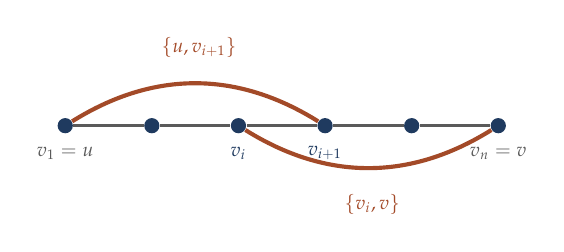
\begin{tikzpicture}[scale=1.0]
\foreach \i/\x in {1/0, 2/1.1, 3/2.2, 4/3.3, 5/4.4, 6/5.5}
  \node[knoten] (w\i) at (\x,0) {};
\foreach \i/\j in {1/2,2/3,4/5,5/6} \draw[kante] (w\i) -- (w\j);
\draw[kante] (w3) -- (w4);
\node[font=\scriptsize, color=grau] at (0,-0.35) {$v_1=u$};
\node[font=\scriptsize, color=tief] at (2.2,-0.35) {$v_i$};
\node[font=\scriptsize, color=tief] at (3.3,-0.35) {$v_{i+1}$};
\node[font=\scriptsize, color=grau] at (5.5,-0.35) {$v_n=v$};
\draw[kanted] (w1) to[bend left=32] (w4);
\draw[kanted] (w3) to[bend right=32] (w6);
\node[font=\scriptsize, color=akzent] at (1.7,1.0) {$\{u,v_{i+1}\}$};
\node[font=\scriptsize, color=akzent] at (3.9,-1.0) {$\{v_i,v\}$};
\end{tikzpicture}
\end{center}

\schritt{Warum das ein Kreis durch alle Ecken ist}
Der erste Abschnitt durchläuft $v_1, \ldots, v_i$; der zweite $v_n, v_{n-1}, \ldots, v_{i+1}$. Zusammen sind das alle $n$ Ecken, jede genau einmal.

Die benutzten Kanten: die Wegkanten $\{v_1,v_2\}, \ldots, \{v_{i-1},v_i\}$ und $\{v_{i+1},v_{i+2}\}, \ldots, \{v_{n-1},v_n\}$ --- sie gehören zum Hamiltonweg. Dazu die Übergangskante $\{v_i, v_n\} = \{v_i, v\}$ und die Schlusskante $\{v_{i+1}, v_1\} = \{v_{i+1}, u\}$ --- beide liegen nach Wahl von $i$ in $G'$.

\schritt{Der Widerspruch}
$G'$ hat also einen Hamiltonkreis --- im Widerspruch zu (b). Die Annahme war falsch. $\blacksquare$
\end{merksatz}

\begin{merksatz}
\boxtitel{Folgerung 7.4 (Dirac 1952)}
Hat jede Ecke eines Graphen mit $n \ge 3$ Ecken mindestens den Grad $n/2$, so ist $G$ hamiltonsch.

\schritt{Beweis}
Für nicht benachbarte $u, v$ gilt
\[ \deg(u) + \deg(v) \;\ge\; \frac{n}{2} + \frac{n}{2} = n . \]
Das ist die Ore-Bedingung. $\blacksquare$

\begin{center}
\begin{minipage}{0.88\textwidth}
\kursiv{Historisch war es umgekehrt: Dirac kam acht Jahre früher, Ore verallgemeinerte. Dass die stärkere Aussage den kürzeren Beweis hat, ist in der Mathematik nicht selten --- eine schärfere Formulierung zeigt oft erst, worauf es wirklich ankommt.}
\end{minipage}
\end{center}
\end{merksatz}

\begin{warnung}
\boxtitelr{Die Schranke $n/2$ ist scharf --- und die Bedingung ist weit von notwendig entfernt}
\schritt{Scharf}
Nimmt man zwei vollständige Graphen $K_{(n+1)/2}$, die genau eine Ecke gemeinsam haben (für ungerades $n$), so hat jede Ecke mindestens Grad $\frac{n-1}{2}$ --- knapp unter $n/2$. Der Graph hat eine Schnittecke und ist nach Satz 7.2 nicht hamiltonsch.

\schritt{Weit von notwendig}
Der Kreis $C_{100}$ ist hamiltonsch --- er \kursiv{ist} sein eigener Hamiltonkreis. Jede Ecke hat aber nur Grad $2$, und $n/2 = 50$. Dirac ist also meilenweit verfehlt.

\begin{center}
\begin{minipage}{0.88\textwidth}
\kursiv{Das ist die Lage bei allen bekannten hinreichenden Bedingungen: Sie verlangen sehr dichte Graphen. Die schwierigen Fälle --- dünne Graphen wie der Petersen-Graph --- werden von keiner erfasst.}
\end{minipage}
\end{center}
\end{warnung}

\section{Der Würfelgraph und die Gray-Codes}

\begin{definition}
\boxtitelm{Definition 7.5 --- Würfelgraph}
Der \Begriff{Würfelgraph} $Q_d$ hat als Ecken alle $2^d$ Folgen aus Nullen und Einsen der Länge $d$. Zwei Ecken sind benachbart, wenn sie sich an genau einer Stelle unterscheiden.
\end{definition}

\begin{merksatz}
\boxtitel{Satz 7.6 --- $Q_d$ ist hamiltonsch für $d \ge 2$}
\schritt{Beweis durch Induktion über $d$}
\textbf{Anfang $d = 2$:} $Q_2$ hat die vier Ecken $00, 01, 11, 10$, und je zwei aufeinanderfolgende unterscheiden sich an einer Stelle. Das ist ein Viereck --- der Hamiltonkreis ist der Graph selbst.

\textbf{Schritt.} Sei $d \ge 3$ und $C$ ein Hamiltonkreis in $Q_{d-1}$.

\schritt{Die Zerlegung}
$Q_d$ besteht aus zwei Kopien von $Q_{d-1}$: der Menge aller Folgen, die mit $0$ beginnen, und der Menge aller, die mit $1$ beginnen. Innerhalb jeder Kopie sind die Nachbarschaften dieselben wie in $Q_{d-1}$ --- die erste Stelle ändert sich ja nicht. Zusätzlich ist jede Ecke $0w$ mit $1w$ benachbart, denn sie unterscheiden sich genau an der ersten Stelle.

\schritt{Der Zusammenbau}
Sei $\{x, y\}$ eine beliebige Kante des Hamiltonkreises $C$. Wir bilden:
\begin{center}
\renewcommand{\arraystretch}{1.45}
\begin{tabular}{@{}P{3.2cm}P{5.4cm}@{}}
\toprule
Kopie $0$ & der Kreis $C$, mit vorangestellter $0$, ohne die Kante $\{0x, 0y\}$ --- ein Weg von $0x$ nach $0y$\\
Kopie $1$ & derselbe Kreis mit vorangestellter $1$, ohne $\{1x, 1y\}$ --- ein Weg von $1x$ nach $1y$\\
Verbindung & die Kanten $\{0x, 1x\}$ und $\{0y, 1y\}$\\
\bottomrule
\end{tabular}
\end{center}

\begin{center}
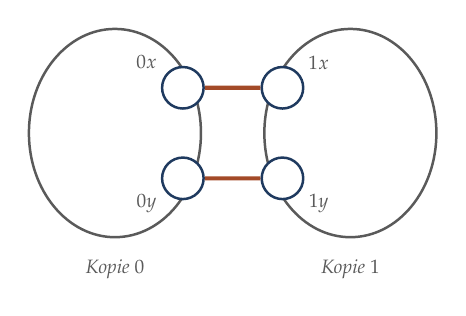
\begin{tikzpicture}[scale=1.15]
\draw[kante] (-1.3,0) ellipse (0.95 and 1.15);
\draw[kante] (1.3,0) ellipse (0.95 and 1.15);
\node[knotenb] (a) at (-0.55,0.5) {};
\node[knotenb] (b) at (-0.55,-0.5) {};
\node[knotenb] (c) at (0.55,0.5) {};
\node[knotenb] (d) at (0.55,-0.5) {};
\draw[kanted] (a)--(c); \draw[kanted] (b)--(d);
\node[font=\scriptsize, color=grau] at (-0.95,0.78) {$0x$};
\node[font=\scriptsize, color=grau] at (-0.95,-0.78) {$0y$};
\node[font=\scriptsize, color=grau] at (0.95,0.78) {$1x$};
\node[font=\scriptsize, color=grau] at (0.95,-0.78) {$1y$};
\node[font=\scriptsize\itshape, color=grau] at (-1.3,-1.5) {Kopie $0$};
\node[font=\scriptsize\itshape, color=grau] at (1.3,-1.5) {Kopie $1$};
\end{tikzpicture}
\end{center}

\schritt{Warum das ein Hamiltonkreis ist}
Wir laufen: von $0x$ über den Weg in Kopie $0$ nach $0y$, dann über $\{0y, 1y\}$ nach $1y$, dann über den Weg in Kopie $1$ nach $1x$, dann über $\{1x, 0x\}$ zurück.

Jede Ecke von Kopie $0$ kommt genau einmal vor (der Weg ist ein Hamiltonweg dieser Kopie), ebenso jede von Kopie $1$. Zusammen alle $2^d$ Ecken, jede genau einmal. $\blacksquare$
\end{merksatz}

\begin{merksatz}
\boxtitel{Was das praktisch bedeutet: Gray-Codes}
Ein Hamiltonkreis in $Q_d$ ist dasselbe wie eine Anordnung aller $2^d$ Bitfolgen der Länge $d$, bei der sich aufeinanderfolgende Folgen an genau einer Stelle unterscheiden --- und die letzte wieder an einer Stelle von der ersten. So etwas heißt \Begriff{Gray-Code}.

\schritt{Der Fall $d = 3$, aus dem Beweis gewonnen}
$Q_2$-Kreis: $00 \to 01 \to 11 \to 10 \to 00$. Wir entfernen die Kante $\{10, 00\}$ und erhalten den Weg $00 \to 01 \to 11 \to 10$.

\begin{center}
\renewcommand{\arraystretch}{1.4}
\begin{tabular}{@{}P{4.2cm}P{4.2cm}@{}}
\toprule
\textbf{Kopie $0$ (vorwärts)} & \textbf{Kopie $1$ (rückwärts)}\\
\midrule
$000, 001, 011, 010$ & $110, 111, 101, 100$\\
\bottomrule
\end{tabular}
\end{center}

Der Gesamtkreis lautet
\[ 000 \to 001 \to 011 \to 010 \to 110 \to 111 \to 101 \to 100 \to 000 . \]

\schritt{Probe}
Wir prüfen jeden Übergang auf genau eine geänderte Stelle:
\begin{center}
{\small
\renewcommand{\arraystretch}{1.32}
\begin{tabular}{@{}P{2.4cm}P{1.8cm}P{2.4cm}P{1.8cm}@{}}
\toprule
\textbf{Übergang} & \textbf{Stelle} & \textbf{Übergang} & \textbf{Stelle}\\
\midrule
$000 \to 001$ & $3$ & $110 \to 111$ & $3$\\
$001 \to 011$ & $2$ & $111 \to 101$ & $2$\\
$011 \to 010$ & $3$ & $101 \to 100$ & $3$\\
$010 \to 110$ & $1$ & $100 \to 000$ & $1$\\
\bottomrule
\end{tabular}}
\end{center}
Acht Übergänge, jeder ändert genau eine Stelle. \checkmark

\begin{center}
\begin{minipage}{0.88\textwidth}
\kursiv{Gray-Codes werden bei Drehgebern verwendet --- etwa in der Winkelmessung. Beim Übergang von einer Stellung zur nächsten ändert sich nur ein einziges Bit; ein Ablesefehler kann daher höchstens eine Stellung danebenliegen. Bei gewöhnlicher Binärzählung geht $011 \to 100$ über drei Bits gleichzeitig, und ein ungünstiger Ablesezeitpunkt liefert einen völlig falschen Wert.}
\end{minipage}
\end{center}
\end{merksatz}

\section{Der Petersen-Graph ist nicht hamiltonsch}

Jetzt die versprochene Abrechnung mit dem Petersen-Graphen. Er erfüllt die Komponentenbedingung, hat keine Schnittecke, ist $3$-regulär und hochsymmetrisch --- und hat trotzdem keinen Hamiltonkreis. Der Beweis ist der erste in diesem Band, der eine Fallunterscheidung über mehrere Seiten braucht.

\begin{merksatz}
\boxtitel{Die Bezeichnungen}
\begin{center}
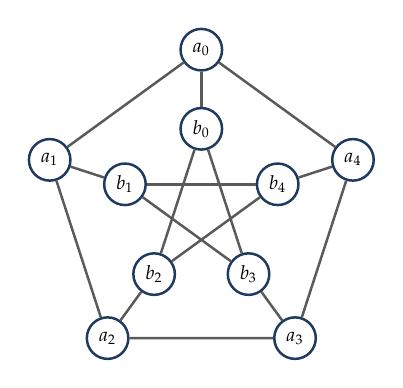
\begin{tikzpicture}[scale=1.5]
\foreach \i in {0,...,4} {
  \node[knotenb] (a\i) at (90+72*\i:1.35) {$a_{\i}$};
  \node[knotenb] (b\i) at (90+72*\i:0.68) {$b_{\i}$};
  \draw[kante] (a\i) -- (b\i);
}
\foreach \i/\j in {0/1,1/2,2/3,3/4,4/0} \draw[kante] (a\i) -- (a\j);
\foreach \i/\j in {0/2,1/3,2/4,3/0,4/1} \draw[kante] (b\i) -- (b\j);
\end{tikzpicture}
\end{center}

\begin{center}
\renewcommand{\arraystretch}{1.45}
\begin{tabular}{@{}P{2.4cm}P{3.0cm}P{2.2cm}@{}}
\toprule
\textbf{Sorte} & \textbf{Kanten} & \textbf{Anzahl}\\
\midrule
Außenkreis & $a_i a_{i+1}$ & $5$\\
Speichen & $a_i b_i$ & $5$\\
Innenstern & $b_i b_{i+2}$ & $5$\\
\bottomrule
\end{tabular}
\end{center}
Alle Indizes werden modulo $5$ gerechnet: $a_5$ bedeutet $a_0$.
\end{merksatz}

\begin{merksatz}
\boxtitel{Hilfssatz 7.7 --- Kreise überqueren einen Schnitt gerade oft}
Sei $C$ ein Kreis in einem Graphen und $A \subseteq V$. Dann ist die Anzahl der Kanten von $C$, die eine Ecke in $A$ und eine außerhalb haben, gerade.

\schritt{Beweis}
Wir laufen den Kreis einmal ab und notieren bei jedem Schritt, ob wir in $A$ oder außerhalb sind. Jede Überquerungskante wechselt die Seite, jede andere nicht.

Da wir am Ende wieder am Ausgangspunkt sind --- also auf derselben Seite wie zu Beginn ---, muss die Anzahl der Seitenwechsel gerade sein. $\blacksquare$
\end{merksatz}

\begin{merksatz}
\boxtitel{Satz 7.8 --- Der Petersen-Graph hat keinen Hamiltonkreis}
\schritt{Annahme}
Sei $H$ ein Hamiltonkreis. Er hat $10$ Ecken und daher $10$ Kanten, und jede Ecke hat in $H$ genau den Grad $2$.

\schritt{Schritt 1 --- Wie viele Speichen benutzt $H$?}
Sei $A = \{a_0, \ldots, a_4\}$ die Außenmenge. Die Kanten zwischen $A$ und dem Rest sind genau die fünf Speichen. Nach Hilfssatz 7.7 benutzt $H$ eine \kursiv{gerade} Anzahl davon. Sei $s$ diese Anzahl; also $s \in \{0, 2, 4\}$.

\schritt{Schritt 2 --- Die Kantenbilanz}
Wir zählen die Grade der Außenecken in $H$. Jede hat Grad $2$, also
\[ \sum_{i} \deg_H(a_i) = 10 . \]
Andererseits setzt sich diese Summe zusammen aus den Enden der benutzten Außenkanten (jede liefert $2$) und den Enden der benutzten Speichen (jede liefert $1$ an der Außenseite):
\[ 2 \cdot |{\text{Außenkanten in } H}| + s = 10 . \]
Also
\[ |{\text{Außenkanten in } H}| = \frac{10 - s}{2} . \]
Dieselbe Rechnung für die Innenecken ergibt denselben Wert für die Innenkanten.

\begin{center}
\renewcommand{\arraystretch}{1.45}
\begin{tabular}{@{}P{1.4cm}P{2.4cm}P{2.4cm}P{1.6cm}@{}}
\toprule
$s$ & \textbf{Außenkanten} & \textbf{Innenkanten} & \textbf{Summe}\\
\midrule
$0$ & $5$ & $5$ & $10$\\
$2$ & $4$ & $4$ & $10$\\
$4$ & $3$ & $3$ & $10$\\
\bottomrule
\end{tabular}
\end{center}
In allen Fällen kommt $10$ heraus, wie es sein muss.
\end{merksatz}

\begin{merksatz}
\boxtitel{Fall $s = 0$}
Dann benutzt $H$ alle fünf Außenkanten und alle fünf Innenkanten, aber keine Speiche.

Die fünf Außenkanten bilden den Kreis $a_0 a_1 a_2 a_3 a_4 a_0$ --- einen geschlossenen Kreis auf nur fünf Ecken. $H$ enthielte damit einen echten Teilkreis, was für einen Kreis mit zehn Ecken unmöglich ist: Ein Kreis hat an jeder Ecke genau zwei Kanten, und wenn fünf Ecken bereits untereinander geschlossen sind, kann keine Kante mehr nach außen führen.

Also ist $s = 0$ ausgeschlossen.
\end{merksatz}

\begin{merksatz}
\boxtitel{Fall $s = 2$}
$H$ benutzt $4$ der $5$ Außenkanten, $4$ der $5$ Innenkanten und $2$ Speichen.

\schritt{Was die Außenkanten bilden}
Vier der fünf Kanten des Kreises $a_0 \ldots a_4$: Das ist der Kreis ohne eine Kante, also ein \kursiv{Weg} durch alle fünf Außenecken. Sei $\{a_k, a_{k+1}\}$ die weggelassene Kante; dann sind die beiden Endecken des Weges genau $a_k$ und $a_{k+1}$.

\schritt{Wo die Speichen ansetzen müssen}
Die Ecken im Inneren des Weges haben schon Grad $2$ durch Außenkanten. Die beiden Endecken $a_k$ und $a_{k+1}$ haben erst Grad $1$ und brauchen je eine weitere Kante --- das können nur Speichen sein.

Die beiden benutzten Speichen sind also $\{a_k, b_k\}$ und $\{a_{k+1}, b_{k+1}\}$.

\schritt{Was innen passieren muss}
Nach demselben Argument bilden die vier Innenkanten einen Weg durch alle fünf Innenecken, und seine beiden Endecken müssen genau die von den Speichen getroffenen sein: $b_k$ und $b_{k+1}$.

\schritt{Der Widerspruch}
Der Innenstern ist der Kreis $b_0 b_2 b_4 b_1 b_3 b_0$. Lässt man daraus eine Kante weg, etwa $\{b_j, b_{j+2}\}$, so sind die Endecken des entstehenden Weges genau $b_j$ und $b_{j+2}$ --- zwei Ecken, deren Indizes sich um $2$ unterscheiden.

Gefordert waren aber $b_k$ und $b_{k+1}$ --- Indizes, die sich um $1$ unterscheiden. Es müsste also
\[ 1 \equiv \pm 2 \pmod 5 \]
gelten. Das ist falsch: $1 \neq 2$ und $1 \neq 3$ modulo $5$.

Also ist $s = 2$ ausgeschlossen.
\end{merksatz}

\begin{merksatz}
\boxtitel{Fall $s = 4$}
$H$ benutzt $3$ Außenkanten, $3$ Innenkanten und $4$ Speichen. Genau eine Speiche fehlt; sei es $\{a_k, b_k\}$. Wir setzen ohne Einschränkung $k = 0$ --- der Graph ist symmetrisch genug, dass man die Nummerierung so drehen darf.

\schritt{Schritt 1 --- Was an $a_0$ und $b_0$ geschieht}
$a_0$ benutzt keine Speiche, hat aber Grad $2$. Die einzigen anderen Kanten an $a_0$ sind $\{a_4, a_0\}$ und $\{a_0, a_1\}$. Beide müssen also in $H$ liegen.

Ebenso muss $b_0$ beide Innenkanten benutzen: $\{b_0, b_2\}$ und $\{b_0, b_3\}$.

\schritt{Schritt 2 --- Die übrigen Außenecken}
$a_1$ benutzt die Speiche $\{a_1,b_1\}$ und hat bereits $\{a_0,a_1\}$. Damit ist Grad $2$ erreicht --- die Kante $\{a_1, a_2\}$ liegt \kursiv{nicht} in $H$.

Ebenso hat $a_4$ die Speiche und $\{a_4,a_0\}$; also liegt $\{a_3,a_4\}$ nicht in $H$.

\schritt{Schritt 3 --- Die dritte Außenkante ist erzwungen}
Bisher zwei Außenkanten ($a_4a_0$ und $a_0a_1$); es müssen drei sein. Von den restlichen drei Außenkanten sind $a_1a_2$ und $a_3a_4$ ausgeschlossen. Bleibt nur $\{a_2, a_3\}$.

Kontrolle: $a_2$ hat dann Speiche und $\{a_2,a_3\}$ --- Grad $2$. \checkmark\ $a_3$ ebenso. \checkmark

\schritt{Schritt 4 --- Die übrigen Innenecken}
$b_2$ hat bereits $\{b_0,b_2\}$ und die Speiche $\{a_2,b_2\}$ --- Grad $2$ erreicht. Ebenso $b_3$.

Bleiben $b_1$ und $b_4$: Beide haben ihre Speiche und brauchen je genau eine Innenkante. Und es fehlt genau eine Innenkante an der Zahl $3$.

Diese eine Kante muss also $b_1$ mit $b_4$ verbinden. Ist $\{b_1, b_4\}$ überhaupt eine Kante? Der Innenstern verbindet $b_i$ mit $b_{i\pm2}$; und $4 \equiv 1 - 2 \pmod 5$. Ja, sie existiert.

\schritt{Schritt 5 --- Alles ist festgelegt --- und falsch}
Es gibt also genau eine Möglichkeit. Die zehn Kanten von $H$ wären:
\begin{center}
\renewcommand{\arraystretch}{1.42}
\begin{tabular}{@{}P{2.4cm}P{5.8cm}@{}}
\toprule
Außen & $a_4a_0$, $a_0a_1$, $a_2a_3$\\
Speichen & $a_1b_1$, $a_2b_2$, $a_3b_3$, $a_4b_4$\\
Innen & $b_0b_2$, $b_0b_3$, $b_1b_4$\\
\bottomrule
\end{tabular}
\end{center}

Jede Ecke hat darin Grad $2$ --- das lässt sich nachprüfen. Aber ist es ein \kursiv{Kreis}?

Wir laufen los bei $a_0$:
\[ a_0 \to a_1 \to b_1 \to b_4 \to a_4 \to a_0 . \]
Nach fünf Schritten sind wir zurück. Das ist ein Kreis der Länge $5$, nicht $10$.

Die übrigen fünf Ecken bilden den zweiten Kreis:
\[ a_2 \to a_3 \to b_3 \to b_0 \to b_2 \to a_2 . \]

\begin{center}
\begin{tikzpicture}[scale=1.5]
\foreach \i in {0,...,4} {
  \node[knotenb] (a\i) at (90+72*\i:1.35) {$a_{\i}$};
  \node[knotenb] (b\i) at (90+72*\i:0.68) {$b_{\i}$};
}
\foreach \i/\j in {0/1,1/2,2/3,3/4,4/0} \draw[kante, grau!35] (a\i) -- (a\j);
\foreach \i/\j in {0/2,1/3,2/4,3/0,4/1} \draw[kante, grau!35] (b\i) -- (b\j);
\foreach \i in {0,...,4} \draw[kante, grau!35] (a\i) -- (b\i);
\draw[kanted] (a4)--(a0); \draw[kanted] (a0)--(a1);
\draw[kanted] (a1)--(b1); \draw[kanted] (b1)--(b4); \draw[kanted] (b4)--(a4);
\draw[kante, gruen, line width=1.5pt] (a2)--(a3);
\draw[kante, gruen, line width=1.5pt] (a3)--(b3); \draw[kante, gruen, line width=1.5pt] (b3)--(b0);
\draw[kante, gruen, line width=1.5pt] (b0)--(b2); \draw[kante, gruen, line width=1.5pt] (b2)--(a2);
\end{tikzpicture}
\end{center}

Es entstehen zwei getrennte Fünfkreise, kein Hamiltonkreis. Also ist auch $s = 4$ ausgeschlossen.

\schritt{Schluss}
Alle drei möglichen Werte von $s$ führen auf einen Widerspruch. Der Petersen-Graph besitzt keinen Hamiltonkreis. $\blacksquare$
\end{merksatz}

\begin{merksatz}
\boxtitel{Und doch fast}
Der Petersen-Graph besitzt einen Hamilton\kursiv{weg}, zum Beispiel
\[ a_0 \to a_1 \to a_2 \to a_3 \to a_4 \to b_4 \to b_1 \to b_3 \to b_0 \to b_2 . \]
Prüfen Sie die Kanten: die vier Außenkanten, die Speiche $a_4b_4$, dann $b_4b_1$ (Differenz $2$), $b_1b_3$ (Differenz $2$), $b_3b_0$ (Differenz $2$), $b_0b_2$ (Differenz $2$). Alle vorhanden, alle zehn Ecken genau einmal. \checkmark

Mehr noch: Entfernt man aus dem Petersen-Graphen eine \kursiv{beliebige} Ecke, so ist der Rest hamiltonsch. Solche Graphen heißen \Begriff{hypohamiltonsch} --- sie sind es selbst nicht, aber jeder ihrer Eckenrestgraphen ist es. Der Petersen-Graph ist der kleinste.
\end{merksatz}

\section{Übungsaufgaben}

\begin{aufgabe}
\boxtitel{Aufgabe 7.1 --- Bipartite Graphen und Hamiltonkreise}
Zeigen Sie: Ist $G$ bipartit mit Bipartition $(A,B)$ und hamiltonsch, so gilt $|A| = |B|$. Folgern Sie, dass $K_{3,4}$ nicht hamiltonsch ist.

\loesung
\schritt{Schritt 1 --- Der Hamiltonkreis wechselt die Seiten}
Sei $H = (v_1, v_2, \ldots, v_n, v_1)$ ein Hamiltonkreis. Jede Kante von $H$ ist eine Kante von $G$, verbindet also eine Ecke aus $A$ mit einer aus $B$.

Aufeinanderfolgende Ecken liegen daher stets auf verschiedenen Seiten. Die Ecken wechseln entlang des Kreises also ab: $A, B, A, B, \ldots$

\schritt{Schritt 2 --- Der Kreis hat gerade Länge}
Nach Satz 2.12 enthält ein bipartiter Graph keinen ungeraden Kreis. Also ist $n$ gerade, sagen wir $n = 2r$.

\schritt{Schritt 3 --- Abzählen}
Bei striktem Abwechseln über $2r$ Ecken liegen genau $r$ Ecken in $A$ und $r$ in $B$. Da der Hamiltonkreis \kursiv{alle} Ecken enthält, ist
\[ |A| = r = |B| . \]

\schritt{Schritt 4 --- Anwendung auf $K_{3,4}$}
Hier ist $|A| = 3$ und $|B| = 4$, also $|A| \neq |B|$. Nach dem Bewiesenen ist $K_{3,4}$ nicht hamiltonsch.

\schritt{Gegenprobe über Satz 7.2}
Wählt man $S = A$ (die drei Ecken), so zerfällt $K_{3,4} - S$ in vier isolierte Ecken:
\[ c(G - S) = 4 \;>\; 3 = |S| . \]
Auch die Komponentenbedingung ist verletzt. Beide Wege führen zum selben Ergebnis. \checkmark

\schritt{Nachbemerkung}
$K_{4,4}$ dagegen \kursiv{ist} hamiltonsch: $a_1 b_1 a_2 b_2 a_3 b_3 a_4 b_4 a_1$. Die Bedingung $|A| = |B|$ ist bei vollständig bipartiten Graphen also nicht nur notwendig, sondern auch hinreichend.
\end{aufgabe}

\begin{aufgabe}
\boxtitel{Aufgabe 7.2 --- Ore prüfen}
Sei $G$ der Graph auf $\{1,\ldots,6\}$ mit den Kanten
\[ 12,\ 13,\ 14,\ 23,\ 25,\ 34,\ 36,\ 45,\ 46,\ 56 . \]
Prüfen Sie die Bedingungen von Dirac und Ore und entscheiden Sie über Hamiltonizität.

\loesung
\schritt{Schritt 1 --- Grade bestimmen}
\begin{center}
\renewcommand{\arraystretch}{1.42}
\begin{tabular}{@{}P{1.2cm}P{3.4cm}P{1.4cm}@{}}
\toprule
\textbf{Ecke} & \textbf{Nachbarn} & $\deg$\\
\midrule
$1$ & $2,3,4$ & $3$\\
$2$ & $1,3,5$ & $3$\\
$3$ & $1,2,4,6$ & $4$\\
$4$ & $1,3,5,6$ & $4$\\
$5$ & $2,4,6$ & $3$\\
$6$ & $3,4,5$ & $3$\\
\bottomrule
\end{tabular}
\end{center}
Probe: $3+3+4+4+3+3 = 20 = 2 \cdot 10$. \checkmark

\schritt{Schritt 2 --- Dirac}
Verlangt: $\deg(v) \ge n/2 = 3$ für alle $v$. Der kleinste Grad ist $3$. \textbf{Dirac ist erfüllt.}

\schritt{Schritt 3 --- Also ist $G$ hamiltonsch}
Nach Folgerung 7.4 besitzt $G$ einen Hamiltonkreis. Das Ergebnis steht damit schon fest; wir suchen ihn trotzdem.

\schritt{Schritt 4 --- Ore zur Kontrolle}
Die nicht benachbarten Paare sind $15$, $16$, $24$, $26$, $35$. Wir prüfen jedes:
\begin{center}
\renewcommand{\arraystretch}{1.4}
\begin{tabular}{@{}P{1.6cm}P{2.8cm}P{1.6cm}@{}}
\toprule
\textbf{Paar} & $\deg + \deg$ & $\ge 6$?\\
\midrule
$1,5$ & $3+3 = 6$ & \checkmark\\
$1,6$ & $3+3 = 6$ & \checkmark\\
$2,4$ & $3+4 = 7$ & \checkmark\\
$2,6$ & $3+3 = 6$ & \checkmark\\
$3,5$ & $4+3 = 7$ & \checkmark\\
\bottomrule
\end{tabular}
\end{center}
Ore ist ebenfalls erfüllt --- wie es sein muss, da Dirac schärfer ist.

\schritt{Schritt 5 --- Einen Hamiltonkreis angeben}
Versuch: $1 \to 2 \to 5 \to 6 \to 3 \to 4 \to 1$.

Kantenprüfung: $12$ \checkmark, $25$ \checkmark, $56$ \checkmark, $63$ \checkmark (in der Liste als $36$), $34$ \checkmark, $41$ \checkmark (als $14$).

Alle sechs Ecken genau einmal, sechs Kanten. \checkmark
\end{aufgabe}

\begin{aufgabe}
\boxtitel{Aufgabe 7.3 --- Ein Graph, den keine der Bedingungen erfasst}
Der Kreis $C_8$ ist hamiltonsch. Zeigen Sie, dass weder Dirac noch Ore das erkennen, und erklären Sie, was das über die Reichweite solcher Sätze aussagt.

\loesung
\schritt{Schritt 1 --- Dirac}
In $C_8$ hat jede Ecke Grad $2$. Verlangt wäre $n/2 = 4$. Also $2 < 4$: \textbf{Dirac greift nicht.}

\schritt{Schritt 2 --- Ore}
Nehmen wir zwei gegenüberliegende Ecken, etwa $v_1$ und $v_5$. Sie sind nicht benachbart, und
\[ \deg(v_1) + \deg(v_5) = 2 + 2 = 4 \;<\; 8 = n . \]
\textbf{Ore greift ebenfalls nicht.}

\schritt{Schritt 3 --- Trotzdem hamiltonsch}
$C_8$ \kursiv{ist} sein eigener Hamiltonkreis: $v_1 v_2 \ldots v_8 v_1$ enthält alle acht Ecken genau einmal.

\schritt{Schritt 4 --- Was daraus folgt}
\begin{center}
\begin{minipage}{0.9\textwidth}
Dirac und Ore sind \kursiv{hinreichende}, nicht notwendige Bedingungen. Sie sagen: \enquote{Wenn dicht genug, dann ja.} Sie sagen nichts über dünne Graphen --- und die interessanten Fälle sind meist dünn.

Zahlenmäßig: Dirac verlangt mindestens $n^2/4$ Kanten. $C_8$ hat $8$. Für $n = 8$ verlangt Dirac $16$. Der Abstand ist ein Faktor $2$, und er wächst mit $n$: Bei $n = 100$ verlangt Dirac $2500$ Kanten, $C_{100}$ hat $100$.
\end{minipage}
\end{center}

\begin{center}
\begin{minipage}{0.86\textwidth}
\kursiv{Man kennt keine hinreichende Bedingung, die \kursiv{alle} hamiltonschen Graphen erfasst und zugleich leicht prüfbar ist --- denn eine solche wäre ein vollständiges Kriterium. Kapitel~15 erklärt, warum das vermutlich unmöglich ist.}
\end{minipage}
\end{center}
\end{aufgabe}

\begin{geschichte}
\boxtitelg{Ein Spielzeug, das sich nicht verkaufte}
\Person{William Rowan Hamilton} (1805--1865) entwickelte 1856 eine algebraische Struktur, die er \kursiv{Icosian Calculus} nannte. Um sie anschaulich zu machen, entwarf er ein Spiel: einen hölzernen Dodekaeder mit zwanzig nummerierten Ecken, an denen Stifte steckten. Die Aufgabe war, mit einer Schnur einen Rundgang durch alle zwanzig Ecken zu legen.

Hamilton verkaufte die Rechte 1859 für fünfundzwanzig Pfund an einen Londoner Spielehändler. Das Spiel war ein Ladenhüter --- es galt als zu leicht. Für den Dodekaeder ist es das auch.

\begin{center}
\begin{minipage}{0.9\textwidth}
\kursiv{Die Frage nach solchen Rundgängen war schon vorher gestellt worden. \Person{Thomas Kirkman} untersuchte 1855 --- ein Jahr vor Hamilton --- systematisch, welche Polyeder einen Rundgang durch alle Ecken zulassen. Sein Aufsatz erschien in den Philosophical Transactions und ist die eigentliche erste Behandlung des Problems. Der Name blieb dennoch an Hamilton hängen.}
\end{minipage}
\end{center}

Der Fairness halber: Hamiltons Beitrag lag weniger im Problem als im algebraischen Rahmen, aus dem es entstand. Der Icosian Calculus ist ein früher Vorläufer der Gruppentheorie --- Band 11, Kapitel~3.
\end{geschichte}

\begin{forschung}
\boxtitelp{Warum es vermutlich kein Kriterium gibt}
Die Frage \enquote{Hat dieser Graph einen Hamiltonkreis?} gehört zu den ersten Problemen, für die \Person{Richard Karp} 1972 die \Begriff{NP-Vollständigkeit} nachwies. Was das bedeutet, entwickelt Band 3 der Informatikreihe; die kurze Fassung lautet:

\begin{center}
\renewcommand{\arraystretch}{1.5}
\begin{tabular}{@{}P{3.0cm}P{5.6cm}@{}}
\toprule
\textbf{Prüfen} & Ist ein Kreis vorgelegt, kann man in wenigen Schritten nachrechnen, ob er passt.\\
\textbf{Finden} & Kein Verfahren bekannt, das ihn in vertretbarer Zeit findet.\\
\textbf{Die Kopplung} & Gäbe es eines, so gäbe es zugleich schnelle Verfahren für Tausende anderer Probleme --- das ist die Frage \enquote{P gleich NP?}.\\
\bottomrule
\end{tabular}
\end{center}

Ein einfaches Kriterium vom Typ des Satzes 6.4 wäre genau so ein Verfahren. Wer eines fände, hätte damit eines der sieben Millenniumsprobleme gelöst.

\begin{center}
\begin{minipage}{0.88\textwidth}
\kursiv{Die Forschung geht deshalb andere Wege. Man untersucht eingeschränkte Graphenklassen, in denen es doch geht, und man untersucht \kursiv{typische} Graphen: In einem Zufallsgraphen mit $n$ Ecken ist ein Hamiltonkreis mit hoher Wahrscheinlichkeit vorhanden, sobald keine Ecke mehr den Grad $0$ oder $1$ hat --- ein Ergebnis von Komlós und Szemerédi (1983), auf das Kapitel~14 zurückkommt. Der schwierige Fall ist also nicht der Regelfall, sondern die Ausnahme.}
\end{minipage}
\end{center}
\end{forschung}

\begin{merksatz}
\boxtitel{Was Sie jetzt können}
\begin{center}
\renewcommand{\arraystretch}{1.5}
\begin{tabular}{@{}P{3.0cm}P{5.6cm}@{}}
\toprule
\textbf{Der Unterschied} & Euler betrifft Kanten und ist gelöst; Hamilton betrifft Ecken und ist es nicht\\
\textbf{Satz 7.2} & Komponentenbedingung --- das Werkzeug zum Widerlegen\\
\textbf{Satz 7.3} & Ore: $\deg(u) + \deg(v) \ge n$ genügt\\
\textbf{Folgerung 7.4} & Dirac als Sonderfall\\
\textbf{Satz 7.6} & $Q_d$ ist hamiltonsch --- Gray-Codes\\
\textbf{Satz 7.8} & Der Petersen-Graph ist es nicht\\
\bottomrule
\end{tabular}
\end{center}

\begin{center}
\begin{minipage}{0.88\textwidth}
\kursiv{Damit endet Teil~III. Ab Kapitel~8 geht es nicht mehr ums Durchlaufen, sondern ums Zeichnen: Wann lässt sich ein Graph ohne Überkreuzungen aufs Papier bringen?}
\end{minipage}
\end{center}
\end{merksatz}

\part{Zeichnen und Färben}

\chapter{Planare Graphen}

\section{Drei Häuser und drei Brunnen}

\begin{merksatz}
\boxtitel{Ein Rätsel aus dem 19. Jahrhundert}
Drei Häuser sollen mit drei Versorgungswerken verbunden werden --- Wasser, Gas, Strom. Jedes Haus braucht eine Leitung zu jedem Werk, also neun Leitungen. Die Leitungen liegen alle in derselben Ebene und dürfen sich nicht kreuzen.

\begin{center}
\begin{tikzpicture}[scale=1.25]
\foreach \i in {0,1,2} {
  \node[knotenb] (h\i) at (-1.2+1.2*\i,0.9) {};
  \node[knotenr] (w\i) at (-1.2+1.2*\i,-0.9) {};
}
\foreach \i in {0,1,2} \foreach \j in {0,1,2} \draw[kante, grau!45] (h\i) -- (w\j);
\node[font=\scriptsize\itshape, color=grau] at (0,1.35) {Häuser};
\node[font=\scriptsize\itshape, color=grau] at (0,-1.35) {Werke};
\end{tikzpicture}
\end{center}

\textbf{Die Frage:} Geht das?
\end{merksatz}

Wer es probiert, kommt regelmäßig bis zur achten Leitung und scheitert an der neunten. Das Rätsel wurde jahrzehntelang in Zeitschriften abgedruckt, ohne dass jemand die Auflösung gab.

Der Graph ist $K_{3,3}$. Am Ende dieses Kapitels werden wir wissen: Es geht nicht --- und zwar aus einem Grund, der sich in vier Zeilen hinschreiben lässt, sobald man die Eulersche Polyederformel hat.

\section{Ebene Zeichnungen}

\begin{definition}
\boxtitelm{Definition 8.1 --- planar, ebene Zeichnung}
Eine \Begriff{ebene Zeichnung} eines Graphen $G$ ordnet
\begin{itemize}[leftmargin=1.4em, itemsep=3pt]
\item jeder Ecke einen Punkt der Ebene zu, verschiedenen Ecken verschiedene Punkte;
\item jeder Kante $\{u,v\}$ eine überschneidungsfreie Kurve, die den Punkt von $u$ mit dem von $v$ verbindet und keinen weiteren Eckenpunkt enthält,
\end{itemize}
so dass sich zwei Kanten\-kurven höchstens in gemeinsamen Endpunkten treffen.

$G$ heißt \Begriff{planar}, wenn er eine ebene Zeichnung besitzt. Ein Graph zusammen mit einer festen ebenen Zeichnung heißt \Begriff{ebener Graph}.
\end{definition}

\begin{warnung}
\boxtitelr{Planar ist eine Eigenschaft des Graphen, nicht der Zeichnung}
Ein Graph ist planar, sobald \kursiv{mindestens eine} kreuzungsfreie Zeichnung existiert. Dass eine bestimmte Zeichnung Kreuzungen hat, sagt gar nichts.

\begin{center}
\begin{tikzpicture}[scale=1.15]
\begin{scope}
\node[knoten] (a1) at (-0.9,0.9) {};
\node[knoten] (a2) at (0.9,0.9) {};
\node[knoten] (a3) at (0.9,-0.9) {};
\node[knoten] (a4) at (-0.9,-0.9) {};
\draw[kante] (a1)--(a2);\draw[kante] (a2)--(a3);\draw[kante] (a3)--(a4);\draw[kante] (a4)--(a1);
\draw[kante] (a1)--(a3);\draw[kante] (a2)--(a4);
\node[font=\scriptsize\itshape, color=akzent] at (0,-1.5) {sieht nach Kreuzung aus};
\end{scope}
\begin{scope}[xshift=5.0cm]
\node[knoten] (b1) at (-0.9,0.9) {};
\node[knoten] (b2) at (0.9,0.9) {};
\node[knoten] (b3) at (0.9,-0.9) {};
\node[knoten] (b4) at (0,0.0) {};
\draw[kante] (b1)--(b2);\draw[kante] (b2)--(b3);
\draw[kante] (b1)--(b4);\draw[kante] (b2)--(b4);\draw[kante] (b3)--(b4);
\draw[kante] (b1) to[bend right=60] (b3);
\node[font=\scriptsize\itshape, color=gruen] at (0,-1.5) {derselbe $K_4$, kreuzungsfrei};
\end{scope}
\end{tikzpicture}
\end{center}

Der $K_4$ ist planar. Man muss nur eine Ecke ins Innere legen.

\begin{center}
\begin{minipage}{0.88\textwidth}
\kursiv{Deshalb ist der Nachweis der \kursiv{Nicht}-Planarität die schwierige Richtung: Man muss zeigen, dass \kursiv{keine} Zeichnung funktioniert --- und davon gibt es unendlich viele. Genau dafür brauchen wir die Polyederformel.}
\end{minipage}
\end{center}
\end{warnung}

\begin{definition}
\boxtitelm{Definition 8.2 --- Gebiete}
Sei eine ebene Zeichnung von $G$ gegeben. Entfernt man alle Eckenpunkte und Kantenkurven aus der Ebene, so zerfällt der Rest in zusammenhängende Stücke. Diese heißen die \Begriff{Gebiete} (oder \Begriff{Flächen}) der Zeichnung. Ihre Anzahl bezeichnen wir mit $f$.
\end{definition}

\begin{merksatz}
\boxtitel{Das äußere Gebiet zählt mit}
Genau ein Gebiet ist unbeschränkt --- das \Begriff{äußere Gebiet}, das sich ins Unendliche erstreckt. Es wird mitgezählt.

\begin{center}
\begin{tikzpicture}[scale=1.3]
\node[knoten] (a) at (-1.0,0.8) {};
\node[knoten] (b) at (1.0,0.8) {};
\node[knoten] (c) at (1.0,-0.8) {};
\node[knoten] (d) at (-1.0,-0.8) {};
\node[knoten] (e) at (0,0) {};
\draw[kante] (a)--(b);\draw[kante] (b)--(c);\draw[kante] (c)--(d);\draw[kante] (d)--(a);
\draw[kante] (a)--(e);\draw[kante] (c)--(e);
\node[font=\scriptsize, color=mittel] at (-0.35,0.35) {$1$};
\node[font=\scriptsize, color=mittel] at (0.35,-0.35) {$2$};
\node[font=\scriptsize, color=mittel] at (1.7,1.1) {$3$};
\node[font=\scriptsize\itshape, color=grau] at (0,-1.3) {$n=5$, $m=6$, $f=3$};
\end{tikzpicture}
\end{center}

Probe: $5 - 6 + 3 = 2$.
\end{merksatz}

\section{Die Eulersche Polyederformel}

\begin{merksatz}
\boxtitel{Satz 8.3 (Euler 1750)}
Für jede ebene Zeichnung eines \kursiv{zusammenhängenden} Graphen mit $n$ Ecken, $m$ Kanten und $f$ Gebieten gilt
\[ n \;-\; m \;+\; f \;=\; 2 . \]
\end{merksatz}

\begin{merksatz}
\boxtitel{Beweis durch Induktion über die Kantenzahl}
\schritt{Induktionsanfang --- der Graph ist ein Baum}
Der Fall mit den wenigsten Kanten bei gegebenem $n$ ist der Baum: $m = n-1$ nach Satz 4.2.

Ein Baum hat genau ein Gebiet, nämlich das äußere. Warum? Ein zusätzliches Gebiet entstünde nur, wenn eine geschlossene Kurve die Ebene zerteilt --- und dafür bräuchte man einen Kreis, den ein Baum nicht hat.

Also
\[ n - m + f = n - (n-1) + 1 = 2 . \quad \checkmark \]

\schritt{Induktionsschritt --- ein Graph mit einem Kreis}
Sei $G$ zusammenhängend und nicht kreisfrei, und sei die Formel für alle zusammenhängenden ebenen Graphen mit weniger Kanten bewiesen.

Sei $e$ eine Kante auf einem Kreis $C$ von $G$.

\schritt{Was das Entfernen von $e$ bewirkt --- die Ecken}
Nichts. $n$ bleibt gleich.

\schritt{Was es bewirkt --- die Kanten}
Eine weniger: $m-1$.

\schritt{Was es bewirkt --- der Zusammenhang}
Nach Satz 2.14 ist $e$ keine Brücke, denn $e$ liegt auf einem Kreis. Also bleibt $G - e$ zusammenhängend.

\schritt{Was es bewirkt --- die Gebiete}
Hier steckt der eigentliche Inhalt. Die Kante $e$ liegt auf dem Kreis $C$. Eine geschlossene, überschneidungsfreie Kurve teilt die Ebene in ein Inneres und ein Äußeres --- das ist der \Begriff{Jordansche Kurvensatz}.

Daraus folgt: Die beiden Seiten von $e$ gehören zu \kursiv{verschiedenen} Gebieten. Denn $e$ ist ein Stück der geschlossenen Kurve $C$; auf der einen Seite liegt Inneres, auf der anderen Äußeres von $C$, und man kann nicht von der einen zur anderen gelangen, ohne $C$ zu überqueren.

Entfernt man $e$, so verschmelzen genau diese beiden Gebiete zu einem. Alle übrigen bleiben unberührt. Also $f - 1$.

\schritt{Zusammenrechnen}
Nach Induktionsannahme gilt für $G-e$:
\[ n - (m-1) + (f-1) = 2 . \]
Ausmultiplizieren:
\[ n - m + 1 + f - 1 = n - m + f = 2 . \qquad \blacksquare \]
\end{merksatz}

\begin{warnung}
\boxtitelr{Was hier ehrlicherweise vorausgesetzt wurde}
Der Beweis benutzt den Jordanschen Kurvensatz: \kursiv{Jede geschlossene, überschneidungsfreie Kurve in der Ebene teilt diese in genau zwei Gebiete.}

Diese Aussage klingt wie eine Selbstverständlichkeit und ist keine. Ihr Beweis ist erheblich schwieriger als alles in diesem Band; \Person{Camille Jordan} gab 1887 einen, der als lückenhaft galt, und ein vollständiger Beweis stammt von \Person{Oswald Veblen} (1905).

\begin{center}
\begin{minipage}{0.88\textwidth}
\kursiv{Nach der Regel dieses Werkes müsste ich ihn führen. Ich tue es nicht --- er gehört in die Topologie und würde den Band sprengen; Band 8 der Reihe behandelt ihn. Was ich stattdessen tue, ist ihn zu \kursiv{benennen}: Sie wissen jetzt, an welcher Stelle dieses Kapitel auf fremdem Boden steht. Ein verschwiegener Schritt wäre schlimmer als ein ausgewiesener.}
\end{minipage}
\end{center}
\end{warnung}

\begin{merksatz}
\boxtitel{Die Formel an Beispielen}
\begin{center}
{\small
\renewcommand{\arraystretch}{1.42}
\begin{tabular}{@{}P{2.6cm}P{1.2cm}P{1.2cm}P{1.2cm}P{1.8cm}@{}}
\toprule
\textbf{Graph} & $n$ & $m$ & $f$ & $n-m+f$\\
\midrule
Dreieck $C_3$ & $3$ & $3$ & $2$ & $2$\\
$K_4$ & $4$ & $6$ & $4$ & $2$\\
Würfel $Q_3$ & $8$ & $12$ & $6$ & $2$\\
Weg $P_5$ & $5$ & $4$ & $1$ & $2$\\
Oktaeder & $6$ & $12$ & $8$ & $2$\\
Dodekaeder & $20$ & $30$ & $12$ & $2$\\
\bottomrule
\end{tabular}}
\end{center}

\begin{center}
\begin{minipage}{0.88\textwidth}
\kursiv{Die Zeilen $3$, $5$ und $6$ betreffen Körper, nicht Zeichnungen. Der Zusammenhang: Die Oberfläche eines konvexen Körpers lässt sich auf die Ebene ausbreiten --- man denke an einen Drahtkäfig, den man an einer Fläche aufschneidet und flach drückt. Diese Fläche wird zum äußeren Gebiet. Deshalb heißt die Formel \enquote{Polyederformel}, obwohl sie hier über Zeichnungen spricht.}
\end{minipage}
\end{center}
\end{merksatz}

\section{Wie viele Kanten passen in die Ebene?}

\begin{merksatz}
\boxtitel{Satz 8.4 --- Die Kantenschranke}
Für jeden planaren Graphen mit $n \ge 3$ Ecken gilt
\[ m \;\le\; 3n - 6 . \]
Ist $G$ zusätzlich dreiecksfrei, so gilt sogar
\[ m \;\le\; 2n - 4 . \]
\end{merksatz}

\begin{merksatz}
\boxtitel{Beweis der ersten Ungleichung}
\schritt{Schritt 0 --- Auf den zusammenhängenden Fall zurückführen}
Ist $G$ unzusammenhängend, so kann man Kanten hinzufügen, bis er zusammenhängend ist, ohne die Planarität zu verlieren (man verbindet zwei Komponenten durch eine Kante durch das äußere Gebiet). Die Kantenzahl wächst dabei; gilt die Schranke für den vollen Graphen, so erst recht für den ursprünglichen. Wir dürfen also $G$ als zusammenhängend annehmen.

Ferner dürfen wir $m \ge 2$ annehmen, sonst ist die Behauptung für $n \ge 3$ trivial.

\schritt{Schritt 1 --- Jedes Gebiet zählen}
Wir zählen Paare $(g, e)$ aus einem Gebiet $g$ und einer Kante $e$, die an $g$ angrenzt. Nennen wir die Anzahl $Z$ --- wieder eine Doppelzählung.

\schritt{Schritt 2 --- Zählung nach Kanten}
Jede Kante grenzt an höchstens zwei Gebiete: an die eine und an die andere Seite. (Bei einer Brücke ist es auf beiden Seiten dasselbe Gebiet; dann grenzt sie nur an eines, zählt aber wegen der zwei Seiten doppelt --- wir zählen Seiten, und davon hat jede Kante genau zwei.)
\[ Z = 2m . \]

\schritt{Schritt 3 --- Zählung nach Gebieten}
Behauptung: Jedes Gebiet wird von mindestens $3$ Kantenseiten begrenzt.

Warum? Der Rand eines Gebiets ist ein geschlossener Kantenzug. Ein solcher hat Länge $\ge 3$, denn:
\begin{itemize}[leftmargin=1.4em, itemsep=2pt]
\item Länge $1$ bräuchte eine Schlinge --- gibt es nicht;
\item Länge $2$ bräuchte zwei parallele Kanten --- gibt es nicht.
\end{itemize}
Bei einer Brücke wird sie beim Umrunden zweimal gezählt, was zulässig ist, weil wir Seiten zählen. Also
\[ Z \;\ge\; 3f . \]

\schritt{Schritt 4 --- Verbinden}
\[ 2m = Z \ge 3f \quad\Longrightarrow\quad f \le \frac{2m}{3} . \]

\schritt{Schritt 5 --- In die Polyederformel einsetzen}
\[ 2 = n - m + f \;\le\; n - m + \frac{2m}{3} = n - \frac{m}{3} . \]
Umstellen:
\[ \frac{m}{3} \le n - 2 \quad\Longrightarrow\quad m \le 3n - 6 . \qquad \blacksquare \]

\schritt{Die zweite Ungleichung --- was sich ändert}
Ist $G$ dreiecksfrei, so hat jeder Gebietsrand Länge $\ge 4$: Länge $3$ wäre ein Dreieck. Also $Z \ge 4f$, somit $f \le m/2$, und
\[ 2 \le n - m + \frac{m}{2} = n - \frac{m}{2} \quad\Longrightarrow\quad m \le 2n - 4 . \qquad \blacksquare \]
\end{merksatz}

\begin{merksatz}
\boxtitel{Satz 8.5 --- $K_5$ und $K_{3,3}$ sind nicht planar}
\schritt{$K_5$}
\begin{center}
\renewcommand{\arraystretch}{1.45}
\begin{tabular}{@{}P{2.4cm}P{2.0cm}P{3.4cm}@{}}
\toprule
Ecken & $n = 5$ & \\
Kanten & $m = \binom{5}{2} = 10$ & \\
Schranke & $3n-6 = 9$ & \\
\midrule
\textbf{Vergleich} & $10 > 9$ & \textcolor{akzent}{\textbf{verletzt}}\\
\bottomrule
\end{tabular}
\end{center}
Nach Satz 8.4 kann $K_5$ nicht planar sein.

\schritt{$K_{3,3}$}
$K_{3,3}$ ist bipartit, enthält also nach Satz 2.12 keinen ungeraden Kreis --- insbesondere kein Dreieck. Die zweite Schranke ist anwendbar:
\begin{center}
\renewcommand{\arraystretch}{1.45}
\begin{tabular}{@{}P{2.4cm}P{2.0cm}P{3.4cm}@{}}
\toprule
Ecken & $n = 6$ & \\
Kanten & $m = 3 \cdot 3 = 9$ & \\
Schranke & $2n-4 = 8$ & \\
\midrule
\textbf{Vergleich} & $9 > 8$ & \textcolor{akzent}{\textbf{verletzt}}\\
\bottomrule
\end{tabular}
\end{center}
$\blacksquare$

\begin{center}
\begin{minipage}{0.9\textwidth}
\textbf{Damit ist das Rätsel der drei Häuser gelöst.} Die neunte Leitung lässt sich nicht kreuzungsfrei legen --- nicht, weil man ungeschickt wäre, sondern weil acht das Maximum ist.
\end{minipage}
\end{center}

\begin{center}
\begin{minipage}{0.88\textwidth}
\kursiv{Beachten Sie, wie kurz der Nachweis am Ende ist: eine Zeile Rechnung je Graph. Die ganze Arbeit steckt in der Polyederformel und in Satz 8.4 --- und die wurden ein für alle Mal erledigt.}
\end{minipage}
\end{center}
\end{merksatz}

\begin{warnung}
\boxtitelr{Die Umkehrung von Satz 8.4 gilt nicht}
Aus $m \le 3n-6$ folgt \kursiv{nicht}, dass $G$ planar ist.

\schritt{Gegenbeispiel}
Man nehme $K_5$ und hänge an eine seiner Ecken einen langen Weg an, sagen wir mit $10$ zusätzlichen Ecken. Dann ist
\[ n = 15, \qquad m = 10 + 10 = 20, \qquad 3n - 6 = 39 . \]
Die Schranke ist bequem erfüllt. Der Graph ist trotzdem nicht planar --- er enthält ja $K_5$.

\begin{center}
\begin{minipage}{0.88\textwidth}
\kursiv{Satz 8.4 ist also ein \kursiv{Ausschlusswerkzeug}, kein Kriterium. Es fängt nur die Graphen, die insgesamt zu viele Kanten haben --- nicht die, bei denen das Problem lokal sitzt.}
\end{minipage}
\end{center}
\end{warnung}

\begin{merksatz}
\boxtitel{Folgerung 8.6 --- Jeder planare Graph hat eine dünne Ecke}
In jedem planaren Graphen gibt es eine Ecke vom Grad höchstens $5$.

\schritt{Beweis}
Für $n \le 6$ ist das klar: Jeder Grad ist höchstens $n - 1 \le 5$.

Sei also $n \ge 7$ und angenommen, jede Ecke hätte Grad $\ge 6$. Dann liefert das Handschlaglemma
\[ 2m = \sum_v \deg(v) \;\ge\; 6n \quad\Longrightarrow\quad m \ge 3n . \]
Nach Satz 8.4 ist aber $m \le 3n-6 < 3n$. Widerspruch. $\blacksquare$

\begin{center}
\begin{minipage}{0.88\textwidth}
\kursiv{Diese unscheinbare Folgerung ist der Angelpunkt des nächsten Kapitels. Der gesamte Fünffarbensatz beruht darauf, dass man immer eine Ecke mit höchstens fünf Nachbarn findet, sie wegnimmt und den Rest per Induktion behandelt.}
\end{minipage}
\end{center}
\end{merksatz}

\section{Der Satz von Kuratowski}

Satz 8.5 zeigt: $K_5$ und $K_{3,3}$ sind die beiden kleinsten nicht planaren Graphen. Kuratowskis Satz sagt, dass sie die \kursiv{einzigen} Hindernisse sind --- jedes andere Hindernis enthält eines der beiden in verkleideter Form.

\begin{definition}
\boxtitelm{Definition 8.7 --- Unterteilung}
Eine \Begriff{Unterteilung} eines Graphen $H$ entsteht, indem man einzelne Kanten von $H$ durch Wege ersetzt: Statt der Kante $\{u,v\}$ setzt man neue Ecken $w_1, \ldots, w_k$ ein und die Kanten $uw_1, w_1w_2, \ldots, w_kv$.
\end{definition}

\begin{merksatz}
\boxtitel{Warum Unterteilungen für die Planarität gleichgültig sind}
\begin{center}
\begin{tikzpicture}[scale=1.2]
\begin{scope}
\node[knoten] (u) at (-0.8,0) {};
\node[knoten] (v) at (0.8,0) {};
\draw[kante] (u)--(v);
\node[font=\scriptsize\itshape, color=grau] at (0,-0.7) {eine Kante};
\end{scope}
\node[font=\large, color=grau] at (1.9,0) {$\rightsquigarrow$};
\begin{scope}[xshift=3.9cm]
\node[knoten] (p) at (-0.9,0) {};
\node[knoten] (q1) at (-0.3,0) {};
\node[knoten] (q2) at (0.3,0) {};
\node[knoten] (r) at (0.9,0) {};
\draw[kante] (p)--(q1);\draw[kante] (q1)--(q2);\draw[kante] (q2)--(r);
\node[font=\scriptsize\itshape, color=grau] at (0,-0.7) {ein Weg};
\end{scope}
\end{tikzpicture}
\end{center}

Eine Kante ist in einer Zeichnung ohnehin eine Kurve. Ob auf dieser Kurve noch zusätzliche Punkte als Ecken markiert sind, ändert an den Kreuzungen nichts.

\textbf{Also:} Ein Graph ist genau dann planar, wenn jede seiner Unterteilungen es ist.
\end{merksatz}

\begin{merksatz}
\boxtitel{Satz 8.8 (Kuratowski 1930)}
Ein Graph ist genau dann planar, wenn er \kursiv{keinen} Teilgraphen enthält, der eine Unterteilung von $K_5$ oder von $K_{3,3}$ ist.
\end{merksatz}

\begin{warnung}
\boxtitelr{Diesen Satz beweise ich nicht}
Die eine Richtung ist leicht --- sie folgt aus Satz 8.5 und der Bemerkung über Unterteilungen: Enthält $G$ eine Unterteilung von $K_5$ oder $K_{3,3}$, so kann $G$ nicht planar sein, weil sonst auch dieser Teilgraph planar wäre.

Die andere Richtung ist schwer. Der kürzeste bekannte Beweis füllt mehrere Seiten und arbeitet mit einer Induktion über die Kantenzahl, in der man sorgfältig durch dreifach zusammenhängende Teile hindurchgehen muss.

\begin{center}
\begin{minipage}{0.88\textwidth}
\kursiv{Ich gebe ihn hier nicht wieder, und ich sage das ausdrücklich, statt es zu verschweigen. Wer ihn sehen will, findet ihn bei Diestel\zit{7}, Kapitel 4 --- vollständig und lesbar. Das Ergebnis selbst brauchen wir im Folgenden nur als Werkzeug.}
\end{minipage}
\end{center}
\end{warnung}

\begin{merksatz}
\boxtitel{Der Satz von Wagner --- dieselbe Aussage, anders formuliert}
Eine \Begriff{Kontraktion} einer Kante $\{u,v\}$ verschmilzt die beiden Ecken zu einer, die mit allen bisherigen Nachbarn von $u$ und $v$ verbunden ist. Ein \Begriff{Minor} von $G$ entsteht durch beliebiges Weglassen von Ecken und Kanten und Kontrahieren von Kanten.

\begin{center}
\begin{tikzpicture}[scale=1.2]
\begin{scope}
\node[knotenb] (u) at (-0.6,0.5) {$u$};
\node[knotenb] (v) at (0.6,0.5) {$v$};
\node[knoten] (x) at (-1.2,-0.6) {};
\node[knoten] (y) at (0,-0.8) {};
\node[knoten] (z) at (1.2,-0.6) {};
\draw[kanted] (u)--(v);
\draw[kante] (u)--(x);\draw[kante] (u)--(y);
\draw[kante] (v)--(y);\draw[kante] (v)--(z);
\end{scope}
\node[font=\large, color=grau] at (2.2,0) {$\rightsquigarrow$};
\begin{scope}[xshift=4.4cm]
\node[knotenr] (w) at (0,0.5) {$w$};
\node[knoten] (x2) at (-1.2,-0.6) {};
\node[knoten] (y2) at (0,-0.8) {};
\node[knoten] (z2) at (1.2,-0.6) {};
\draw[kante] (w)--(x2);\draw[kante] (w)--(y2);\draw[kante] (w)--(z2);
\end{scope}
\end{tikzpicture}
\end{center}

\textbf{Satz (Wagner 1937).} Ein Graph ist genau dann planar, wenn er weder $K_5$ noch $K_{3,3}$ als Minor enthält.

\begin{center}
\begin{minipage}{0.88\textwidth}
\kursiv{Die beiden Fassungen sind gleichwertig, aber die Minor-Fassung erwies sich als die tragfähigere: Sie ist der Ausgangspunkt der Graphenminorentheorie von Robertson und Seymour, einem der umfangreichsten Beweiswerke der Mathematik überhaupt. Kapitel~15 berichtet davon.}
\end{minipage}
\end{center}
\end{merksatz}

\section{Übungsaufgaben}

\begin{aufgabe}
\boxtitel{Aufgabe 8.1 --- Der Petersen-Graph}
Ist der Petersen-Graph planar?

\loesung
\schritt{Schritt 1 --- Die Kantenschranke prüfen}
$n = 10$, $m = 15$. Die Schranke lautet $3n-6 = 24$. Wegen $15 \le 24$ ist \kursiv{nichts} ausgeschlossen.

\schritt{Schritt 2 --- Die schärfere Schranke prüfen}
In Aufgabe 2.2 wurde gezeigt: Der Petersen-Graph hat Taille $5$, ist also insbesondere dreiecksfrei. Damit greift die zweite Schranke:
\[ 2n - 4 = 20 . \]
Wegen $15 \le 20$ wieder kein Ausschluss.

\schritt{Schritt 3 --- Noch schärfer: die Taille ausnutzen}
Wir wiederholen den Beweis von Satz 8.4 mit Taille $5$. Jeder Gebietsrand hat dann Länge $\ge 5$, also
\[ 2m \ge 5f \quad\Longrightarrow\quad f \le \frac{2m}{5} . \]
Einsetzen in die Polyederformel:
\[ 2 = n - m + f \le n - m + \frac{2m}{5} = n - \frac{3m}{5} . \]
Umstellen:
\[ \frac{3m}{5} \le n-2 \quad\Longrightarrow\quad m \le \frac{5(n-2)}{3} . \]

Für $n = 10$:
\[ m \le \frac{5 \cdot 8}{3} = \frac{40}{3} = 13{,}33\ldots \]
Da $m$ ganzzahlig ist: $m \le 13$.

\schritt{Schritt 4 --- Der Widerspruch}
Der Petersen-Graph hat $m = 15 > 13$. \textbf{Er ist nicht planar.}

\schritt{Schritt 5 --- Kontrolle über Kuratowski}
Der Petersen-Graph enthält tatsächlich eine Unterteilung des $K_{3,3}$. Man kann sie so finden: Die drei Ecken $a_0, b_1, b_4$ bilden die eine Seite, die drei Ecken $a_1, a_4, b_0$ die andere; die neun Verbindungen laufen teils direkt, teils über je eine Zwischenecke. Die Ausarbeitung ist mühsam --- und genau deshalb ist die Rechnung aus Schritt 3 der bessere Weg.

\begin{center}
\begin{minipage}{0.86\textwidth}
\kursiv{Die Verschärfung in Schritt 3 lohnt sich zu merken: \textbf{Bei Taille $g$ gilt $m \le \frac{g(n-2)}{g-2}$.} Für $g=3$ ergibt das $3n-6$, für $g=4$ ergibt es $2n-4$ --- beide Schranken aus Satz 8.4 sind Sonderfälle.}
\end{minipage}
\end{center}
\end{aufgabe}

\begin{aufgabe}
\boxtitel{Aufgabe 8.2 --- Ein Polyeder aus Fünfecken}
Ein konvexer Körper habe nur fünfeckige Flächen, und an jeder Ecke sollen genau drei Flächen zusammenstoßen. Wie viele Ecken, Kanten und Flächen hat er?

\loesung
\schritt{Schritt 1 --- Die Kanten aus den Flächen}
Jede Fläche wird von $5$ Kanten begrenzt, und jede Kante grenzt an genau $2$ Flächen. Zählen wir Paare (Fläche, angrenzende Kante):
\[ 5f = 2m \quad\Longrightarrow\quad m = \frac{5f}{2} . \]

\schritt{Schritt 2 --- Die Kanten aus den Ecken}
An jeder Ecke stoßen $3$ Flächen zusammen, also auch $3$ Kanten. Jede Kante hat $2$ Enden:
\[ 3n = 2m \quad\Longrightarrow\quad n = \frac{2m}{3} . \]

\schritt{Schritt 3 --- In die Polyederformel}
\[ n - m + f = 2 \]
Wir drücken alles durch $m$ aus. Aus Schritt 1: $f = \frac{2m}{5}$. Aus Schritt 2: $n = \frac{2m}{3}$.
\[ \frac{2m}{3} - m + \frac{2m}{5} = 2 \]

\schritt{Schritt 4 --- Auflösen}
Hauptnenner $15$:
\[ \frac{10m}{15} - \frac{15m}{15} + \frac{6m}{15} = 2 \]
\[ \frac{10m - 15m + 6m}{15} = \frac{m}{15} = 2 \]
\[ m = 30 . \]

\schritt{Schritt 5 --- Die übrigen Größen}
\[ n = \frac{2 \cdot 30}{3} = 20, \qquad f = \frac{2 \cdot 30}{5} = 12 . \]

\schritt{Probe}
$20 - 30 + 12 = 2$. \checkmark\quad Und $5 \cdot 12 = 60 = 2 \cdot 30$ \checkmark,\quad $3 \cdot 20 = 60 = 2 \cdot 30$ \checkmark

\schritt{Antwort}
$20$ Ecken, $30$ Kanten, $12$ Fünfecke --- das ist der \textbf{Dodekaeder}. Und es ist der einzige Körper dieser Bauart: Die Rechnung hatte keine Freiheit, das Ergebnis war erzwungen.

\begin{center}
\begin{minipage}{0.86\textwidth}
\kursiv{Genau so beweist man, dass es nur fünf platonische Körper gibt: Man setzt \enquote{alle Flächen sind $k$-Ecke, an jeder Ecke stoßen $r$ zusammen} an und rechnet nach, für welche Paare $(k,r)$ die Polyederformel eine positive Lösung hat. Es sind fünf.}
\end{minipage}
\end{center}
\end{aufgabe}

\begin{aufgabe}
\boxtitel{Aufgabe 8.3 --- $K_{3,3}$ ohne eine Kante}
Ist $K_{3,3}$ minus einer beliebigen Kante planar? Zeichnen Sie gegebenenfalls.

\loesung
\schritt{Schritt 1 --- Die Zahlen}
$n = 6$, $m = 8$. Dreiecksfrei (Teilgraph eines bipartiten Graphen ist bipartit). Schranke: $2n-4 = 8$.

Wegen $8 \le 8$ ist nichts ausgeschlossen --- die Schranke wird exakt erreicht. Das ist ein Hinweis, dass es gehen könnte, aber kein Beweis.

\schritt{Schritt 2 --- Eine Zeichnung angeben}
Wir lassen die Kante $\{h_3, w_3\}$ weg.

\begin{center}
\begin{tikzpicture}[scale=1.4]
\node[knotenb] (h1) at (-1.3,0.9) {$h_1$};
\node[knotenb] (w1) at (0,1.5) {$w_1$};
\node[knotenb] (h2) at (1.3,0.9) {$h_2$};
\node[knotenb] (w2) at (1.3,-0.7) {$w_2$};
\node[knotenb] (h3) at (0,-1.3) {$h_3$};
\node[knotenb] (w3) at (-1.3,-0.7) {$w_3$};
\draw[kante] (h1)--(w1); \draw[kante] (w1)--(h2); \draw[kante] (h2)--(w2);
\draw[kante] (w2)--(h3); \draw[kante] (h3)--(w3); \draw[kante] (w3)--(h1);
\draw[kante] (h1) to[bend right=18] (w2);
\draw[kante] (h2) to[bend right=18] (w3);
\end{tikzpicture}
\end{center}

\schritt{Schritt 3 --- Nachprüfen, dass alles da ist}
Verlangt sind alle Paare $h_i w_j$ außer $h_3w_3$:
\begin{center}
{\small
\renewcommand{\arraystretch}{1.35}
\begin{tabular}{@{}P{1.6cm}P{2.6cm}P{2.6cm}@{}}
\toprule
& $w_1$ & $w_2$\\
\midrule
$h_1$ & Außenkante & Sehne\\
$h_2$ & Außenkante & Außenkante\\
$h_3$ & \multicolumn{2}{@{}l}{$h_3 w_1$? --- \textcolor{akzent}{fehlt!}}\\
\bottomrule
\end{tabular}}
\end{center}

Halt. Im Sechseck $h_1 w_1 h_2 w_2 h_3 w_3$ sind die Nachbarn von $h_3$ nur $w_2$ und $w_3$; die Kante $h_3w_1$ fehlt, und die haben wir nicht weggelassen.

\schritt{Schritt 4 --- Korrektur}
Wir zählen neu. Das Sechseck liefert $6$ Kanten, die beiden Sehnen $2$ weitere --- zusammen $8$. Gebraucht werden $8$. Es fehlt also genau eine der neun, und wir müssen prüfen \kursiv{welche}.

Vorhanden sind: $h_1w_1$, $w_1h_2$, $h_2w_2$, $w_2h_3$, $h_3w_3$, $w_3h_1$ (Sechseck) sowie $h_1w_2$ und $h_2w_3$ (Sehnen).

Fehlend ist somit $h_3w_1$ --- nicht $h_3w_3$, wie in Schritt 2 angekündigt.

Das macht nichts: Die Frage lautete, ob $K_{3,3}$ minus \kursiv{einer beliebigen} Kante planar ist, und $K_{3,3}$ ist so symmetrisch, dass alle neun Kanten gleichwertig sind. Die Zeichnung zeigt $K_{3,3} - h_3w_1$, und das beantwortet die Frage.

\schritt{Antwort}
\textbf{Ja, planar.} Die Zeichnung hat $n=6$, $m=8$ und --- nach der Polyederformel --- $f = 2 - n + m = 4$ Gebiete: das Äußere und drei innere.

\begin{center}
\begin{minipage}{0.86\textwidth}
\kursiv{Die Korrektur in Schritt 4 habe ich stehen lassen, statt sie stillschweigend auszubessern. So läuft mathematisches Arbeiten wirklich ab: Man zeichnet, prüft nach, findet eine Abweichung von der Ankündigung und schaut, ob sie schadet. Hier schadet sie nicht --- aber das musste geprüft werden.}
\end{minipage}
\end{center}
\end{aufgabe}

\begin{geschichte}
\boxtitelg{Descartes, Euler und eine Formel mit zwei Vätern}
Euler teilte die Formel 1750 in einem Brief an Christian Goldbach mit und veröffentlichte sie 1752. Sein Beweis war unvollständig; einen tragfähigen gab \Person{Adrien-Marie Legendre} 1794 mit einem Argument über Kugelflächen.

Etwa hundert Jahre vor Euler hatte \Person{René Descartes} in einem unveröffentlichten Manuskript eine gleichwertige Aussage über Winkelsummen an Polyederecken notiert. Das Manuskript ging verloren; eine Abschrift von Leibniz wurde erst 1860 wiedergefunden.

\begin{center}
{\small
\renewcommand{\arraystretch}{1.42}
\begin{tabular}{@{}P{1.6cm}P{2.4cm}P{3.8cm}@{}}
\toprule
\textbf{um 1630} & Descartes & gleichwertige Fassung, unveröffentlicht\\
\textbf{1750} & Euler & die Formel, Beweis lückenhaft\\
\textbf{1794} & Legendre & erster tragfähiger Beweis\\
\textbf{1813} & Cauchy & der heute übliche Beweis\\
\bottomrule
\end{tabular}}
\end{center}

\begin{center}
\begin{minipage}{0.9\textwidth}
\kursiv{Bemerkenswert ist der lange Weg von der Formel zum Beweis --- über sechzig Jahre. Der Grund ist derselbe wie bei Hierholzer in Kapitel~6: Die Aussage ist anschaulich so überzeugend, dass die Lücke lange niemandem auffiel.}
\end{minipage}
\end{center}
\end{geschichte}

\begin{forschung}
\boxtitelp{Planarität erkennen und Kreuzungen zählen}
\begin{center}
{\small
\renewcommand{\arraystretch}{1.45}
\begin{tabular}{@{}P{3.0cm}P{2.2cm}P{3.0cm}@{}}
\toprule
\textbf{Frage} & \textbf{Aufwand} & \textbf{Stand}\\
\midrule
Ist $G$ planar? & \textcolor{gruen}{$\Oh(n)$} & Hopcroft/Tarjan 1974\\
Ebene Zeichnung finden & \textcolor{gruen}{$\Oh(n)$} & dasselbe Verfahren\\
\textbf{Kleinste Kreuzungszahl} & \textcolor{akzent}{NP-schwer} & Garey/Johnson 1983\\
Kreuzungszahl von $K_n$ & \textcolor{akzent}{offen} & Vermutung seit 1960\\
\bottomrule
\end{tabular}}
\end{center}

Die dritte und vierte Zeile überraschen im Kontrast zur ersten. Ob ein Graph \kursiv{ohne} Kreuzungen gezeichnet werden kann, entscheidet man in linearer Zeit. Wie viele Kreuzungen mindestens nötig sind, wenn es nicht geht, ist eine der hartnäckigsten offenen Fragen des Gebiets.

Für den vollständigen Graphen lautet die Vermutung von Hill und Guy (1960): Die kleinste Kreuzungszahl von $K_n$ beträgt
\[ \frac{1}{4}\Bigl\lfloor \frac{n}{2}\Bigr\rfloor \Bigl\lfloor \frac{n-1}{2}\Bigr\rfloor \Bigl\lfloor \frac{n-2}{2}\Bigr\rfloor \Bigl\lfloor \frac{n-3}{2}\Bigr\rfloor . \]
Bewiesen ist sie bis $n = 12$; die Zeichnungen, die den vermuteten Wert erreichen, sind bekannt --- niemand konnte bisher zeigen, dass es nicht besser geht.

\begin{center}
\begin{minipage}{0.88\textwidth}
\kursiv{Die Kreuzungszahl ist keine Spielerei. Beim Entwurf von Schaltkreisen bestimmt sie, wie viele Ebenen eine Platine braucht, und in der Netzwerkdarstellung entscheidet sie über die Lesbarkeit eines Diagramms.}
\end{minipage}
\end{center}
\end{forschung}

\begin{merksatz}
\boxtitel{Was Sie jetzt können}
\begin{center}
\renewcommand{\arraystretch}{1.5}
\begin{tabular}{@{}P{3.0cm}P{5.6cm}@{}}
\toprule
\textbf{Satz 8.3} & $n - m + f = 2$ für zusammenhängende ebene Graphen\\
\textbf{Satz 8.4} & $m \le 3n-6$, dreiecksfrei $m \le 2n-4$, allgemein $m \le \frac{g(n-2)}{g-2}$\\
\textbf{Satz 8.5} & $K_5$ und $K_{3,3}$ sind nicht planar --- das Rätsel ist gelöst\\
\textbf{Folgerung 8.6} & Jeder planare Graph hat eine Ecke vom Grad $\le 5$\\
\textbf{Satz 8.8} & Kuratowski: nur diese beiden Hindernisse\\
\bottomrule
\end{tabular}
\end{center}

\begin{center}
\begin{minipage}{0.88\textwidth}
\kursiv{Folgerung 8.6 ist der Schlüssel zum nächsten Kapitel --- dort wird sie den Fünffarbensatz tragen.}
\end{minipage}
\end{center}
\end{merksatz}

\chapter{Färbungen}

\section{Der Dienstplan, endlich beantwortet}

In Kapitel 1 stand die zweite Frage: Fünf Ärztinnen, sechs unverträgliche Paare, wie viele Schichten braucht man mindestens? Jetzt haben wir die Mittel.

\begin{definition}
\boxtitelm{Definition 9.1 --- Färbung, chromatische Zahl}
Sei $G = (V,E)$ ein Graph und $k$ eine natürliche Zahl. Eine \Begriff{$k$-Färbung} von $G$ ist eine Abbildung
\[ c : V \longrightarrow \{1, 2, \ldots, k\} \]
mit der Eigenschaft
\[ \{u,v\} \in E \;\Longrightarrow\; c(u) \neq c(v) . \]
Existiert eine solche, so heißt $G$ \Begriff{$k$-färbbar}. Die \Begriff{chromatische Zahl} $\chi(G)$ ist das kleinste $k$, für das $G$ $k$-färbbar ist.
\end{definition}

\begin{warnung}
\boxtitelr{Was die Definition \kursiv{nicht} verlangt}
\begin{center}
\renewcommand{\arraystretch}{1.5}
\begin{tabular}{@{}P{3.4cm}P{5.2cm}@{}}
\toprule
Alle Farben benutzen & nein --- eine $5$-Färbung darf mit drei Farben auskommen\\
Nachbarn verschieden & \textcolor{gruen}{ja, das ist die einzige Forderung}\\
Nichtnachbarn gleich & nein --- sie \kursiv{dürfen} gleich sein, müssen aber nicht\\
\bottomrule
\end{tabular}
\end{center}

Insbesondere ist jede $k$-Färbung auch eine $(k+1)$-Färbung. Die Eigenschaft \enquote{$k$-färbbar} vererbt sich nach oben, und deshalb ist die Frage nach dem \kursiv{kleinsten} $k$ die einzig interessante.
\end{warnung}

\begin{merksatz}
\boxtitel{Der Dienstplan}
Graph: $V = \{A,B,C,D,E\}$, Kanten $AB$, $AC$, $BC$, $BD$, $CE$, $DE$.

\schritt{Schritt 1 --- Eine untere Schranke}
Die drei Ecken $A$, $B$, $C$ sind paarweise benachbart. In jeder Färbung müssen sie drei verschiedene Farben tragen. Also
\[ \chi \ge 3 . \]

\schritt{Schritt 2 --- Eine Färbung mit drei Farben angeben}
\begin{center}
\renewcommand{\arraystretch}{1.42}
\begin{tabular}{@{}P{1.4cm}P{1.4cm}P{1.4cm}P{1.4cm}P{1.4cm}@{}}
\toprule
$A$ & $B$ & $C$ & $D$ & $E$\\
\midrule
$1$ & $2$ & $3$ & $1$ & $2$\\
\bottomrule
\end{tabular}
\end{center}

\schritt{Schritt 3 --- Jede Kante prüfen}
\begin{center}
{\small
\renewcommand{\arraystretch}{1.35}
\begin{tabular}{@{}P{1.4cm}P{1.8cm}P{1.4cm}P{1.8cm}@{}}
\toprule
\textbf{Kante} & \textbf{Farben} & \textbf{Kante} & \textbf{Farben}\\
\midrule
$AB$ & $1 \neq 2$ \checkmark & $BD$ & $2 \neq 1$ \checkmark\\
$AC$ & $1 \neq 3$ \checkmark & $CE$ & $3 \neq 2$ \checkmark\\
$BC$ & $2 \neq 3$ \checkmark & $DE$ & $1 \neq 2$ \checkmark\\
\bottomrule
\end{tabular}}
\end{center}

\schritt{Antwort}
$\chi = 3$: \textbf{Drei Schichten genügen und drei sind nötig.}

\begin{center}
\begin{tikzpicture}[scale=1.35]
\node[knotenb] (A) at (90:1.2) {$A$};
\node[knotenr] (B) at (162:1.2) {$B$};
\node[knoteng] (C) at (18:1.2) {$C$};
\node[knotenb] (D) at (234:1.2) {$D$};
\node[knotenr] (E) at (306:1.2) {$E$};
\draw[kante] (A)--(B);\draw[kante] (A)--(C);\draw[kante] (B)--(C);
\draw[kante] (B)--(D);\draw[kante] (C)--(E);\draw[kante] (D)--(E);
\end{tikzpicture}
\end{center}

\begin{center}
\begin{minipage}{0.88\textwidth}
\kursiv{Beachten Sie den Aufbau der Antwort. Für eine chromatische Zahl braucht man \kursiv{immer zwei Dinge}: eine Färbung, die zeigt, dass es reicht --- und ein Argument, das zeigt, dass weniger nicht geht. Nur eines von beiden genügt nie.}
\end{minipage}
\end{center}
\end{merksatz}

\section{Erste Werte und erste Schranken}

\begin{merksatz}
\boxtitel{Was man sofort ausrechnen kann}
\begin{center}
{\small
\renewcommand{\arraystretch}{1.48}
\begin{tabular}{@{}P{2.4cm}P{1.6cm}P{4.4cm}@{}}
\toprule
\textbf{Graph} & $\chi$ & \textbf{Begründung}\\
\midrule
Leerer Graph & $1$ & keine Kante, alles eine Farbe\\
$K_n$ & $n$ & alle paarweise benachbart\\
Baum ($n\ge2$) & $2$ & bipartit --- Satz 2.12, kein Kreis\\
$C_n$, $n$ gerade & $2$ & bipartit\\
$C_n$, $n$ ungerade & $\mathbf{3}$ & siehe unten\\
$K_{r,s}$ & $2$ & bipartit\\
Petersen & $3$ & siehe Aufgabe 9.2\\
\bottomrule
\end{tabular}}
\end{center}

\schritt{Der ungerade Kreis, nachgerechnet}
Sei $n$ ungerade. Zwei Farben genügen nicht: Nach Satz 2.12 ist $\chi(G) = 2$ gleichbedeutend mit Bipartitheit --- eine $2$-Färbung \kursiv{ist} eine Bipartition ---, und ein ungerader Kreis ist nicht bipartit.

Drei genügen: Man färbt $v_1, v_2, \ldots, v_{n-1}$ abwechselnd mit $1, 2, 1, 2, \ldots$ Da $n-1$ gerade ist, endet das mit $c(v_{n-1}) = 2$. Für $v_n$ nimmt man Farbe $3$; seine Nachbarn $v_{n-1}$ und $v_1$ tragen $2$ und $1$. \checkmark
\end{merksatz}

\begin{definition}
\boxtitelm{Definition 9.2 --- Clique und Unabhängigkeit}
\begin{itemize}[leftmargin=1.4em, itemsep=3pt]
\item Eine \Begriff{Clique} ist eine Eckenmenge, deren Ecken paarweise benachbart sind. Die \Begriff{Cliquenzahl} $\omega(G)$ ist die Größe einer größten Clique.
\item Eine \Begriff{unabhängige Menge} ist eine Eckenmenge ohne Kante dazwischen. Die \Begriff{Unabhängigkeitszahl} $\alpha(G)$ ist die Größe einer größten unabhängigen Menge.
\end{itemize}
\end{definition}

\begin{merksatz}
\boxtitel{Satz 9.3 --- Zwei untere Schranken}
Für jeden Graphen gilt
\[ \chi(G) \;\ge\; \omega(G) \qquad \text{und} \qquad \chi(G) \;\ge\; \frac{n}{\alpha(G)} . \]

\schritt{Beweis der ersten}
Sei $S$ eine Clique der Größe $\omega$. Je zwei Ecken von $S$ sind benachbart, tragen also verschiedene Farben. Somit braucht man mindestens $\omega$ Farben.

\schritt{Beweis der zweiten}
Sei eine $\chi$-Färbung gegeben. Für jede Farbe $i$ sei $V_i$ die Menge der Ecken dieser Farbe.

$V_i$ ist unabhängig: Zwei Ecken darin haben dieselbe Farbe, dürfen also nach Definition 9.1 nicht benachbart sein. Damit ist $|V_i| \le \alpha$.

Jede Ecke liegt in genau einem $V_i$, also
\[ n = \sum_{i=1}^{\chi} |V_i| \;\le\; \chi \cdot \alpha \quad\Longrightarrow\quad \chi \ge \frac{n}{\alpha} . \qquad \blacksquare \]
\end{merksatz}

\begin{warnung}
\boxtitelr{Die erste Schranke kann beliebig schlecht sein}
Man könnte hoffen: $\chi = \omega$. Das wäre bequem, denn Cliquen sieht man.

Es stimmt nicht. Der ungerade Kreis $C_5$ hat $\omega = 2$ (keine drei paarweise benachbarten Ecken) und $\chi = 3$.

Schlimmer: \Person{Jan Mycielski} gab 1955 ein Verfahren an, das aus einem dreiecksfreien Graphen mit chromatischer Zahl $k$ einen dreiecksfreien mit $k+1$ macht. Es gibt also dreiecksfreie Graphen --- $\omega = 2$ --- mit beliebig großer chromatischer Zahl.

\begin{center}
\begin{minipage}{0.88\textwidth}
\kursiv{Das ist eine der überraschendsten Tatsachen des Gebiets. Man würde erwarten, dass eine hohe chromatische Zahl von dicht verwobenen Stellen herrührt. Sie kann aber auch aus großräumiger Struktur kommen, ohne dass irgendwo drei Ecken paarweise benachbart wären.}
\end{minipage}
\end{center}
\end{warnung}

\section{Das gierige Verfahren}

\begin{merksatz}
\boxtitel{Das Verfahren}
\begin{center}
\renewcommand{\arraystretch}{1.5}
\begin{tabular}{@{}P{1.2cm}P{7.2cm}@{}}
\toprule
1. & Bringe die Ecken in eine Reihenfolge $v_1, v_2, \ldots, v_n$.\\
2. & Gehe sie der Reihe nach durch. Gib $v_i$ die kleinste Farbe, die noch bei keinem bereits gefärbten Nachbarn vorkommt.\\
\bottomrule
\end{tabular}
\end{center}
\end{merksatz}

\begin{merksatz}
\boxtitel{Satz 9.4 --- Die Gradschranke}
Sei $\Delta(G)$ der größte in $G$ vorkommende Grad. Dann gilt
\[ \chi(G) \;\le\; \Delta(G) + 1 . \]

\schritt{Beweis}
Wir wenden das gierige Verfahren mit beliebiger Reihenfolge an und behaupten: Es benutzt nie eine Farbe größer als $\Delta + 1$.

Betrachte den Schritt, in dem $v_i$ gefärbt wird. Die Ecke $v_i$ hat höchstens $\Delta$ Nachbarn, also erst recht höchstens $\Delta$ bereits gefärbte Nachbarn. Diese belegen höchstens $\Delta$ verschiedene Farben.

Unter den $\Delta + 1$ Farben $1, 2, \ldots, \Delta+1$ bleibt somit mindestens eine frei. Das Verfahren wählt die kleinste freie und kommt also mit $\Delta+1$ Farben aus.

Dass das Ergebnis eine zulässige Färbung ist, liegt an der Vorschrift: $v_i$ bekommt keine Farbe eines bereits gefärbten Nachbarn, und die später gefärbten Nachbarn meiden ihrerseits die Farbe von $v_i$. $\blacksquare$
\end{merksatz}

\begin{warnung}
\boxtitelr{Die Reihenfolge entscheidet über die Güte}
Das gierige Verfahren liefert \kursiv{immer} eine zulässige Färbung, aber nicht immer eine sparsame.

\begin{center}
\begin{tikzpicture}[scale=1.3]
\node[knotenb] (a1) at (-1.2,0.7) {$1$};
\node[knotenb] (a2) at (-1.2,-0.7) {$3$};
\node[knotenb] (b1) at (0,0.7) {$2$};
\node[knotenb] (b2) at (0,-0.7) {$4$};
\node[knotenb] (c1) at (1.2,0.7) {$5$};
\node[knotenb] (c2) at (1.2,-0.7) {$6$};
\draw[kante] (a1)--(b2); \draw[kante] (a1)--(c2);
\draw[kante] (a2)--(b1); \draw[kante] (a2)--(c1);
\draw[kante] (b1)--(c2); \draw[kante] (b2)--(c1);
\node[font=\scriptsize\itshape, color=grau] at (0,-1.3) {$K_{3,3}$ ohne die \enquote{senkrechten} Kanten};
\end{tikzpicture}
\end{center}

Der Graph ist bipartit --- obere Reihe gegen untere ---, also $\chi = 2$.

\schritt{Ungünstige Reihenfolge}
Nimmt man die Ecken in der Reihenfolge $1,2,3,4,5,6$ wie beschriftet, so ergibt sich:
\begin{center}
{\small
\renewcommand{\arraystretch}{1.35}
\begin{tabular}{@{}P{1.2cm}P{3.0cm}P{1.6cm}@{}}
\toprule
\textbf{Ecke} & \textbf{gefärbte Nachbarn} & \textbf{Farbe}\\
\midrule
$1$ & --- & $1$\\
$2$ & --- & $1$\\
$3$ & $2$ (Farbe $1$) & $2$\\
$4$ & $1$ (Farbe $1$) & $2$\\
$5$ & $3$ (Farbe $2$), $4$ (Farbe $2$) & $1$\\
$6$ & $1$ ($1$), $2$ ($1$) & $2$\\
\bottomrule
\end{tabular}}
\end{center}
Hier ging es gut: zwei Farben. Bei anderer Anordnung derselben Kantenmenge kann das gierige Verfahren jedoch beliebig viele Farben verbrauchen --- es gibt bipartite Graphen, bei denen eine ungeschickte Reihenfolge $n/2$ Farben erzwingt.

\begin{center}
\begin{minipage}{0.88\textwidth}
\kursiv{Es gibt \kursiv{immer} eine Reihenfolge, bei der das gierige Verfahren genau $\chi(G)$ Farben verbraucht --- man ordne die Ecken einer optimalen Färbung nach Farbklassen. Diese Reihenfolge zu finden setzt aber voraus, dass man die optimale Färbung schon kennt. Der Satz ist wahr und nutzlos.}
\end{minipage}
\end{center}
\end{warnung}

\begin{merksatz}
\boxtitel{Satz 9.5 (Brooks 1941)}
Sei $G$ zusammenhängend. Ist $G$ weder ein vollständiger Graph noch ein Kreis ungerader Länge, so gilt
\[ \chi(G) \;\le\; \Delta(G) . \]

\schritt{Warum die beiden Ausnahmen nötig sind}
\begin{center}
\renewcommand{\arraystretch}{1.45}
\begin{tabular}{@{}P{2.2cm}P{1.6cm}P{1.6cm}P{2.4cm}@{}}
\toprule
& $\Delta$ & $\chi$ & \\
\midrule
$K_n$ & $n-1$ & $n$ & \textcolor{akzent}{$\chi = \Delta+1$}\\
$C_5$ & $2$ & $3$ & \textcolor{akzent}{$\chi = \Delta+1$}\\
Petersen & $3$ & $3$ & \textcolor{gruen}{$\chi = \Delta$}\\
$C_6$ & $2$ & $2$ & \textcolor{gruen}{$\chi = \Delta$}\\
\bottomrule
\end{tabular}
\end{center}

Bei den beiden Ausnahmen wird die Schranke aus Satz 9.4 tatsächlich erreicht. Brooks sagt: Sonst nie.
\end{merksatz}

\begin{warnung}
\boxtitelr{Auch diesen Satz beweise ich nicht}
Der Beweis ist nicht schwer im Sinne von tief, aber er zerfällt in eine größere Zahl von Fällen: Man unterscheidet nach $\Delta \le 2$, nach dem Vorhandensein einer Schnittecke und danach, ob der Graph dreifach zusammenhängend ist. Jeder Fall braucht eine eigene Reihenfolge für das gierige Verfahren.

Ich verweise auf Diestel\zit{7}, Kapitel 5. Wie bei Kuratowski gilt: Das Ergebnis brauchen wir nur als Werkzeug, und ein ausgewiesener Verweis ist ehrlicher als ein zusammengeschnurrter Beweis.

\begin{center}
\begin{minipage}{0.88\textwidth}
\kursiv{Das Folgende --- der Fünffarbensatz --- beweise ich dagegen vollständig. Er ist der Höhepunkt dieses Kapitels, und er kommt ohne fremde Hilfsmittel aus.}
\end{minipage}
\end{center}
\end{warnung}

\section{Der Fünffarbensatz}

\begin{merksatz}
\boxtitel{Satz 9.6 (Heawood 1890)}
Jeder planare Graph ist $5$-färbbar.
\end{merksatz}

\begin{merksatz}
\boxtitel{Vorbereitung --- die Kempe-Kette}
Sei eine Färbung eines Graphen gegeben und seien $i \neq j$ zwei Farben. Der \Begriff{$(i,j)$-Teilgraph} ist der von allen Ecken der Farbe $i$ oder $j$ induzierte Teilgraph.

\schritt{Die entscheidende Beobachtung}
Sei $K$ eine Zusammenhangskomponente des $(i,j)$-Teilgraphen. Vertauscht man \kursiv{innerhalb von $K$} die Farben $i$ und $j$ --- also: jede Ecke von $K$ mit Farbe $i$ bekommt $j$ und umgekehrt ---, so bleibt die Färbung zulässig.

\schritt{Warum}
Zu prüfen ist jede Kante $\{x,y\}$.
\begin{center}
\renewcommand{\arraystretch}{1.5}
\begin{tabular}{@{}P{2.6cm}P{6.0cm}@{}}
\toprule
Beide außerhalb $K$ & Nichts ändert sich.\\
Beide in $K$ & Beide werden umgefärbt. Waren sie vorher verschieden ($i$ und $j$), sind sie es nachher auch ($j$ und $i$).\\
$x \in K$, $y \notin K$ & Dann trägt $y$ weder $i$ noch $j$. Denn hätte $y$ eine dieser Farben, so läge $y$ im $(i,j)$-Teilgraphen und wäre über die Kante mit $x$ verbunden --- also in derselben Komponente $K$. Die neue Farbe von $x$ ist $i$ oder $j$, also verschieden von der von $y$.\\
\bottomrule
\end{tabular}
\end{center}
$\blacksquare$

\begin{center}
\begin{tikzpicture}[scale=1.1]
\draw[kante, grau!40] (-0.9,0) ellipse (1.3 and 0.95);
\node[knotenb] (p) at (-1.6,0.25) {$i$};
\node[knotenr] (q) at (-0.9,-0.35) {$j$};
\node[knotenb] (r) at (-0.2,0.25) {$i$};
\draw[kante] (p)--(q); \draw[kante] (q)--(r);
\node[knoteng] (s) at (1.5,0) {$k$};
\draw[kante] (r)--(s);
\node[font=\scriptsize\itshape, color=grau] at (-0.9,-1.35) {Komponente $K$ --- hier wird getauscht};
\node[font=\scriptsize\itshape, color=grau] at (1.5,-1.35) {außerhalb: Farbe $\neq i,j$};
\end{tikzpicture}
\end{center}
\end{merksatz}

\begin{merksatz}
\boxtitel{Beweis des Fünffarbensatzes --- Induktion über $n$}
\schritt{Induktionsanfang}
Für $n \le 5$ färbt man jede Ecke anders; fünf Farben reichen.

\schritt{Induktionsschritt --- die dünne Ecke}
Sei $n \ge 6$ und $G$ planar, und sei der Satz für alle planaren Graphen mit weniger Ecken bewiesen.

Nach Folgerung 8.6 gibt es eine Ecke $v$ mit $\deg(v) \le 5$.

Der Graph $G - v$ ist planar (ein Teilgraph eines planaren Graphen ist planar) und hat $n-1$ Ecken. Nach Induktionsannahme besitzt er eine $5$-Färbung $c$.

\schritt{Fall 1 --- die Nachbarn benutzen höchstens vier Farben}
Dann ist eine der fünf Farben bei den Nachbarn von $v$ unbenutzt. Wir geben $v$ diese Farbe und sind fertig.

Das erledigt insbesondere alle Fälle mit $\deg(v) \le 4$.

\schritt{Fall 2 --- die Vorbereitung}
Bleibt: $\deg(v) = 5$ und die fünf Nachbarn tragen fünf verschiedene Farben.

Wir fixieren eine ebene Zeichnung von $G$. Um $v$ herum liegen die fünf Nachbarn in einer bestimmten zyklischen Reihenfolge; wir nennen sie im Uhrzeigersinn
\[ v_1,\ v_2,\ v_3,\ v_4,\ v_5 \]
und dürfen die Farben so benennen, dass $c(v_i) = i$ gilt.

\begin{center}
\begin{tikzpicture}[scale=1.35]
\node[knotenr] (v) at (0,0) {$v$};
\foreach \i in {1,...,5} {
  \pgfmathsetmacro{\ang}{90-72*(\i-1)}
  \node[knotenb] (n\i) at (\ang:1.35) {$v_{\i}$};
  \draw[kante] (v) -- (n\i);
}
\node[font=\scriptsize, color=grau] at (90:1.75) {Farbe $1$};
\node[font=\scriptsize, color=grau] at (18:1.85) {Farbe $2$};
\node[font=\scriptsize, color=grau] at (-54:1.85) {Farbe $3$};
\node[font=\scriptsize, color=grau] at (-126:1.85) {Farbe $4$};
\node[font=\scriptsize, color=grau] at (162:1.85) {Farbe $5$};
\end{tikzpicture}
\end{center}
\end{merksatz}

\begin{merksatz}
\boxtitel{Beweis --- Fall 2, erster Versuch}
Betrachte den $(1,3)$-Teilgraphen von $G-v$, also alle Ecken der Farben $1$ und $3$.

\schritt{Unterfall 2a --- $v_1$ und $v_3$ liegen in verschiedenen Komponenten}
Sei $K$ die Komponente, die $v_1$ enthält. Wir vertauschen in $K$ die Farben $1$ und $3$. Nach der Vorbereitung bleibt die Färbung zulässig.

Was ist jetzt anders? $v_1$ trägt nun Farbe $3$. Und $v_3$? Es liegt \kursiv{nicht} in $K$, wurde also nicht umgefärbt und trägt weiterhin $3$.

Die Nachbarn von $v$ tragen nun die Farben $3, 2, 3, 4, 5$ --- die Farbe $1$ kommt bei keinem mehr vor. Wir geben $v$ die Farbe $1$. Fertig.

\begin{center}
\begin{minipage}{0.88\textwidth}
\kursiv{Das ist der Kern des Kempe-Tricks: Man ändert die Färbung des Restes so, dass eine Farbe frei wird --- ohne die Zulässigkeit zu zerstören.}
\end{minipage}
\end{center}
\end{merksatz}

\begin{merksatz}
\boxtitel{Beweis --- Fall 2, der schwierige Unterfall}
\schritt{Unterfall 2b --- $v_1$ und $v_3$ liegen in derselben Komponente}
Dann gibt es in $G-v$ einen Weg $P$ von $v_1$ nach $v_3$, auf dem sich die Farben $1$ und $3$ abwechseln --- eine \Begriff{Kempe-Kette}.

\schritt{Der Kreis, der entsteht}
Fügen wir zu $P$ die beiden Kanten $\{v, v_1\}$ und $\{v, v_3\}$ hinzu, so entsteht ein Kreis
\[ C = v \to v_1 \to \cdots \to v_3 \to v . \]

\begin{center}
\begin{tikzpicture}[scale=1.4]
\node[knotenr] (v) at (0,0) {$v$};
\foreach \i in {1,...,5} {
  \pgfmathsetmacro{\ang}{90-72*(\i-1)}
  \node[knotenb] (n\i) at (\ang:1.3) {$v_{\i}$};
}
\draw[kante] (v)--(n2); \draw[kante] (v)--(n4); \draw[kante] (v)--(n5);
\draw[kanted] (v)--(n1); \draw[kanted] (v)--(n3);
\draw[kanted] (n1) to[bend left=55] (n3);
\node[font=\scriptsize, color=akzent] at (2.0,0.35) {Kempe-Kette $P$};
\node[font=\scriptsize\itshape, color=gruen] at (-1.55,-0.9) {$v_4$ liegt außerhalb};
\end{tikzpicture}
\end{center}

\schritt{Was der Kreis trennt}
Nach dem Jordanschen Kurvensatz teilt $C$ die Ebene in ein Inneres und ein Äußeres.

Die Ecke $v_2$ liegt --- in der zyklischen Anordnung um $v$ --- \kursiv{zwischen} $v_1$ und $v_3$; die Ecken $v_4$ und $v_5$ liegen auf der anderen Seite. Da die Kanten $\{v,v_2\}$, $\{v,v_4\}$, $\{v,v_5\}$ von $v$ ausgehen und sich nicht mit $C$ kreuzen dürfen, liegt $v_2$ auf der einen Seite von $C$ und $v_4$ auf der anderen.

\schritt{Der zweite Kempe-Griff}
Betrachte nun den $(2,4)$-Teilgraphen. Läge $v_2$ mit $v_4$ in derselben Komponente, so gäbe es einen Weg $Q$ von $v_2$ nach $v_4$, dessen Ecken abwechselnd die Farben $2$ und $4$ tragen.

Dieser Weg müsste von der einen Seite von $C$ auf die andere gelangen, also $C$ überqueren. Das geht nur über eine Ecke von $C$ --- Kanten dürfen sich in einer ebenen Zeichnung nicht kreuzen.

Die Ecken von $C$ sind aber $v$ (nicht gefärbt, gehört nicht zu $G-v$) und die Ecken von $P$, die alle Farbe $1$ oder $3$ tragen. Keine davon hat Farbe $2$ oder $4$, kann also nicht auf $Q$ liegen.

Widerspruch. Also liegen $v_2$ und $v_4$ in \kursiv{verschiedenen} Komponenten des $(2,4)$-Teilgraphen.

\schritt{Der Abschluss}
Wir vertauschen die Farben $2$ und $4$ in der Komponente, die $v_2$ enthält. Danach trägt $v_2$ die Farbe $4$, während $v_4$ unverändert $4$ trägt.

Die Nachbarn von $v$ tragen nun $1, 4, 3, 4, 5$. Die Farbe $2$ ist frei. Wir geben sie $v$. $\blacksquare$
\end{merksatz}

\begin{merksatz}
\boxtitel{Was dieser Beweis geleistet hat}
\begin{center}
\renewcommand{\arraystretch}{1.5}
\begin{tabular}{@{}P{3.0cm}P{5.6cm}@{}}
\toprule
Aus Kapitel 8 & Folgerung 8.6: eine Ecke vom Grad $\le 5$\\
Aus Kapitel 8 & Der Jordansche Kurvensatz --- schon dort ausgewiesen\\
Neu & Die Kempe-Kette und der doppelte Farbtausch\\
\bottomrule
\end{tabular}
\end{center}

\begin{center}
\begin{minipage}{0.88\textwidth}
\kursiv{Der Beweis ist kurz, vollständig und benutzt kein Hilfsmittel, das nicht in diesem Band steht. Umso bemerkenswerter ist, dass der Schritt von fünf auf vier Farben über hundert Jahre gekostet hat --- und am Ende ganz anders aussah.}
\end{minipage}
\end{center}
\end{merksatz}

\section{Der Vierfarbensatz}

\begin{merksatz}
\boxtitel{Satz 9.7 (Appel und Haken 1976)}
Jeder planare Graph ist $4$-färbbar.
\end{merksatz}

\begin{geschichte}
\boxtitelg{Ein Beweis, der elf Jahre lang für richtig gehalten wurde}
\begin{center}
{\small
\renewcommand{\arraystretch}{1.42}
\begin{tabular}{@{}P{1.6cm}P{2.2cm}P{4.0cm}@{}}
\toprule
\textbf{Jahr} & \textbf{Person} & \textbf{Ereignis}\\
\midrule
$1852$ & Guthrie & stellt die Frage beim Kartenfärben\\
$1879$ & Kempe & veröffentlicht einen \enquote{Beweis}\\
$1890$ & Heawood & findet den Fehler --- rettet den Fünffarbensatz\\
$1913$ & Birkhoff & Methode der reduziblen Konfigurationen\\
$1976$ & Appel, Haken & Beweis mit Rechnerhilfe\\
$1997$ & Robertson u.\,a. & vereinfachter Beweis, $633$ Konfigurationen\\
$2005$ & Gonthier & vollständige maschinelle Verifikation\\
\bottomrule
\end{tabular}}
\end{center}

\Person{Alfred Kempe} führte 1879 genau die Kette vor, die wir eben benutzt haben --- und wandte sie auf den Fall $\deg(v) = 5$ mit vier Farben an. Dort muss man \kursiv{zwei} Vertauschungen nacheinander vornehmen, und Kempe übersah, dass die zweite die erste zunichtemachen kann.

\Person{Percy Heawood} fand den Fehler elf Jahre später. Er konnte ihn nicht reparieren --- aber er bemerkte, dass Kempes Argument für \kursiv{fünf} Farben einwandfrei durchgeht. So entstand der Satz, den wir eben bewiesen haben: als Rettungsstück aus einem gescheiterten Beweis.

\begin{center}
\begin{minipage}{0.9\textwidth}
\kursiv{Kempes Fehler steckte nicht in einer Rechnung, sondern in einer unausgesprochenen Annahme --- er hielt für unabhängig, was es nicht war. Genau davor warnt das Vorwort dieses Bandes.}
\end{minipage}
\end{center}
\end{geschichte}

\begin{forschung}
\boxtitelp{Ein Beweis, den kein Mensch nachlesen kann}
Appel und Haken zeigten 1976: Es gibt eine endliche Liste von \enquote{unvermeidbaren} Konfigurationen --- jeder minimale Gegenbeispielgraph müsste eine davon enthalten --- und jede davon ist \enquote{reduzibel}, führt also auf einen kleineren Gegenbeispielgraphen. Damit kann es keinen minimalen Gegenbeispielgraphen geben.

\begin{center}
{\small
\renewcommand{\arraystretch}{1.45}
\begin{tabular}{@{}P{3.0cm}P{2.2cm}P{2.8cm}@{}}
\toprule
& \textbf{1976} & \textbf{1997}\\
\midrule
Konfigurationen & $1482$ & $633$\\
Rechenzeit & $\approx 1200$ h & $\approx 3$ h\\
Von Hand prüfbar & \textcolor{akzent}{nein} & \textcolor{akzent}{nein}\\
\bottomrule
\end{tabular}}
\end{center}

Das löste eine Debatte aus, die bis heute nachwirkt: Ist ein Beweis, den kein Mensch vollständig durchsehen kann, ein Beweis?

\begin{center}
\renewcommand{\arraystretch}{1.5}
\begin{tabular}{@{}P{2.4cm}P{6.2cm}@{}}
\toprule
\textbf{Dagegen} & Ein Beweis soll Einsicht verschaffen, nicht bloß Gewissheit. Hier versteht man am Ende nicht, \kursiv{warum} vier Farben genügen.\\
\textbf{Dafür} & Die Fehleranfälligkeit langer Handrechnungen ist nachweislich höher als die geprüfter Programme. Kempes Beweis stand elf Jahre.\\
\bottomrule
\end{tabular}
\end{center}

\Person{Georges Gonthier} beendete 2005 den technischen Teil der Debatte: Er formalisierte den gesamten Beweis im Beweisassistenten Coq --- einschließlich der kombinatorischen Argumente und der Fallprüfungen. Die Korrektheit hängt seither nur noch am Kern des Prüfsystems, nicht mehr an einzelnen Programmen.

\begin{center}
\begin{minipage}{0.88\textwidth}
\kursiv{Der philosophische Teil der Debatte bleibt offen. Bis heute kennt niemand einen Beweis des Vierfarbensatzes, den man in einer Vorlesung führen könnte --- und viele Fachleute halten es für möglich, dass es keinen gibt.}
\end{minipage}
\end{center}
\end{forschung}

\section{Übungsaufgaben}

\begin{aufgabe}
\boxtitel{Aufgabe 9.1 --- Chromatische Zahl bestimmen}
Bestimmen Sie $\chi$ für den abgebildeten Graphen und begründen Sie beide Richtungen.

\begin{center}
\begin{tikzpicture}[scale=1.3]
\node[knotenb] (1) at (90:1.2) {$1$};
\node[knotenb] (2) at (162:1.2) {$2$};
\node[knotenb] (3) at (234:1.2) {$3$};
\node[knotenb] (4) at (306:1.2) {$4$};
\node[knotenb] (5) at (18:1.2) {$5$};
\node[knotenb] (6) at (0,0) {$6$};
\draw[kante] (1)--(2);\draw[kante] (2)--(3);\draw[kante] (3)--(4);
\draw[kante] (4)--(5);\draw[kante] (5)--(1);
\draw[kante] (6)--(1);\draw[kante] (6)--(2);\draw[kante] (6)--(3);
\draw[kante] (6)--(4);\draw[kante] (6)--(5);
\end{tikzpicture}
\end{center}

\loesung
\schritt{Schritt 1 --- Was der Graph ist}
Ein Fünfeck $C_5$ mit einer zusätzlichen Ecke $6$, die mit allen fünf verbunden ist. Solche Graphen heißen \Begriff{Rad}.

\schritt{Schritt 2 --- Untere Schranke über eine Clique}
Die Ecken $1$, $2$ und $6$ sind paarweise benachbart: $12$ \checkmark, $16$ \checkmark, $26$ \checkmark. Also $\omega \ge 3$ und damit $\chi \ge 3$ nach Satz 9.3.

\schritt{Schritt 3 --- Die Schranke $3$ genügt nicht}
Angenommen, es gäbe eine $3$-Färbung. Die Ecke $6$ trage Farbe $3$.

Alle fünf Ecken $1, \ldots, 5$ sind mit $6$ benachbart, dürfen also die Farbe $3$ nicht tragen. Sie müssen mit den Farben $1$ und $2$ auskommen.

Die Ecken $1, \ldots, 5$ bilden aber einen $C_5$, und der ist nach Satz 2.12 nicht bipartit --- er braucht drei Farben. Zwei genügen nicht.

Widerspruch. Also $\chi \ge 4$.

\schritt{Schritt 4 --- Vier Farben genügen}
\begin{center}
\renewcommand{\arraystretch}{1.42}
\begin{tabular}{@{}P{1.2cm}P{1.2cm}P{1.2cm}P{1.2cm}P{1.2cm}P{1.2cm}@{}}
\toprule
$1$ & $2$ & $3$ & $4$ & $5$ & $6$\\
\midrule
$1$ & $2$ & $1$ & $2$ & $3$ & $4$\\
\bottomrule
\end{tabular}
\end{center}

Prüfung der Fünfeckskanten: $12$: $1\neq2$ \checkmark; $23$: $2\neq1$ \checkmark; $34$: $1\neq2$ \checkmark; $45$: $2\neq3$ \checkmark; $51$: $3\neq1$ \checkmark.\\
Prüfung der Speichen: Ecke $6$ trägt $4$, alle anderen tragen $1$, $2$ oder $3$. \checkmark

\schritt{Antwort}
$\chi = \mathbf{4}$.

\schritt{Kontrolle über Brooks}
$\Delta = 5$ (die Ecke $6$). Der Graph ist zusammenhängend, kein vollständiger Graph (etwa $\{1,3\}$ ist keine Kante) und kein ungerader Kreis. Brooks liefert $\chi \le 5$ --- richtig, aber nicht scharf. Unsere Rechnung ist genauer.
\end{aufgabe}

\begin{aufgabe}
\boxtitel{Aufgabe 9.2 --- Der Petersen-Graph}
Zeigen Sie $\chi(\text{Petersen}) = 3$.

\loesung
\schritt{Schritt 1 --- Untere Schranke}
Der Petersen-Graph hat Taille $5$ (Aufgabe 2.2), enthält also kein Dreieck --- somit $\omega = 2$, und Satz 9.3 liefert nur $\chi \ge 2$.

Wir brauchen die zweite Schranke. Gilt $\chi = 2$, so wäre der Graph bipartit, hätte also nach Satz 2.12 keinen ungeraden Kreis. Er hat aber Fünfkreise, etwa den Außenkreis. Also $\chi \ge 3$.

\schritt{Schritt 2 --- Drei Farben genügen}
Wir färben mit den Farben $1,2,3$:
\begin{center}
{\small
\renewcommand{\arraystretch}{1.4}
\begin{tabular}{@{}P{1.6cm}P{0.9cm}P{0.9cm}P{0.9cm}P{0.9cm}P{0.9cm}@{}}
\toprule
& $0$ & $1$ & $2$ & $3$ & $4$\\
\midrule
außen $a_i$ & $1$ & $2$ & $1$ & $2$ & $3$\\
innen $b_i$ & $2$ & $3$ & $3$ & $1$ & $1$\\
\bottomrule
\end{tabular}}
\end{center}

\schritt{Schritt 3 --- Alle fünfzehn Kanten prüfen}
\kursiv{Außenkreis $a_ia_{i+1}$:}
\begin{center}
{\small
\renewcommand{\arraystretch}{1.32}
\begin{tabular}{@{}P{1.6cm}P{1.6cm}P{1.6cm}P{1.6cm}P{1.6cm}@{}}
\toprule
$a_0a_1$ & $a_1a_2$ & $a_2a_3$ & $a_3a_4$ & $a_4a_0$\\
$1\neq2$ & $2\neq1$ & $1\neq2$ & $2\neq3$ & $3\neq1$\\
\bottomrule
\end{tabular}}
\end{center}

\kursiv{Speichen $a_ib_i$:}
\begin{center}
{\small
\renewcommand{\arraystretch}{1.32}
\begin{tabular}{@{}P{1.6cm}P{1.6cm}P{1.6cm}P{1.6cm}P{1.6cm}@{}}
\toprule
$a_0b_0$ & $a_1b_1$ & $a_2b_2$ & $a_3b_3$ & $a_4b_4$\\
$1\neq2$ & $2\neq3$ & $1\neq3$ & $2\neq1$ & $3\neq1$\\
\bottomrule
\end{tabular}}
\end{center}

\kursiv{Innenstern $b_ib_{i+2}$:}
\begin{center}
{\small
\renewcommand{\arraystretch}{1.32}
\begin{tabular}{@{}P{1.6cm}P{1.6cm}P{1.6cm}P{1.6cm}P{1.6cm}@{}}
\toprule
$b_0b_2$ & $b_1b_3$ & $b_2b_4$ & $b_3b_0$ & $b_4b_1$\\
$2\neq3$ & $3\neq1$ & $3\neq1$ & $1\neq2$ & $1\neq3$\\
\bottomrule
\end{tabular}}
\end{center}

Alle fünfzehn Kanten in Ordnung. \checkmark

\schritt{Antwort}
$\chi(\text{Petersen}) = \mathbf{3}$.

\begin{center}
\begin{minipage}{0.86\textwidth}
\kursiv{Beachten Sie: Der Petersen-Graph ist \kursiv{nicht} planar (Aufgabe 8.1). Dass er trotzdem mit drei Farben auskommt, ist kein Widerspruch --- der Vierfarbensatz gibt eine obere Schranke für planare Graphen, sagt aber nichts über nichtplanare in die eine oder andere Richtung.}
\end{minipage}
\end{center}
\end{aufgabe}

\begin{aufgabe}
\boxtitel{Aufgabe 9.3 --- Wo Kempes Beweis scheitert}
Erklären Sie genau, warum das Argument aus dem Fünffarbensatz mit \kursiv{vier} Farben nicht durchgeht.

\loesung
\schritt{Schritt 1 --- Die Ausgangslage bei vier Farben}
Man nimmt eine Ecke $v$ mit $\deg(v) \le 5$. Bei $\deg(v) \le 3$ oder wenn die Nachbarn höchstens drei Farben benutzen, ist man fertig.

Der schwierige Fall ist $\deg(v) = 5$ mit vier verschiedenen Farben bei fünf Nachbarn --- eine Farbe kommt also doppelt vor. Sagen wir, die Nachbarn im Uhrzeigersinn tragen
\[ v_1: 1, \quad v_2: 2, \quad v_3: 3, \quad v_4: 4, \quad v_5: 2 . \]

\schritt{Schritt 2 --- Der erste Griff}
Man betrachtet den $(1,3)$-Teilgraphen. Liegen $v_1$ und $v_3$ in verschiedenen Komponenten, tauscht man und macht Farbe $1$ frei. Fertig.

Andernfalls gibt es eine $(1,3)$-Kette von $v_1$ nach $v_3$, die zusammen mit $v$ einen Kreis $C_{13}$ bildet.

\schritt{Schritt 3 --- Der zweite Griff}
Ebenso betrachtet man den $(1,4)$-Teilgraphen. Liegen $v_1$ und $v_4$ in verschiedenen Komponenten, tauscht man dort und ist fertig.

Andernfalls gibt es eine $(1,4)$-Kette von $v_1$ nach $v_4$ mit Kreis $C_{14}$.

\schritt{Schritt 4 --- Kempes Schluss}
Kempe argumentierte: $C_{13}$ trennt $v_2$ von $v_4$, und $C_{14}$ trennt $v_3$ von $v_5$. Also liegen $v_2$ und $v_4$ in verschiedenen Komponenten des $(2,4)$-Teilgraphen, und ebenso $v_3$ und $v_5$ im $(3,2)$-Teilgraphen. Er vertauschte in \kursiv{beiden} Komponenten --- bei $v_2$ die Farben $2$ und $4$, bei $v_3$ die Farben $3$ und $2$ --- und schloss, dass danach Farbe $2$ frei sei.

\schritt{Schritt 5 --- Der Fehler}
Die beiden Vertauschungen sind nicht unabhängig voneinander.

Die erste Vertauschung ändert Farben von $2$ auf $4$ und umgekehrt. Sie kann dadurch den $(3,2)$-Teilgraphen \kursiv{verändern}: Eine Ecke, die vorher Farbe $2$ trug und den Weg von $v_3$ zu $v_5$ blockierte, trägt nachher Farbe $4$ --- und der Weg ist offen. Die zweite Vertauschung setzt dann auf einer Lage auf, die nicht mehr gilt.

\begin{center}
\begin{minipage}{0.88\textwidth}
\kursiv{Heawood konstruierte 1890 genau ein solches Beispiel und zeigte damit, dass Kempes Argument nicht trägt.}
\end{minipage}
\end{center}

\schritt{Schritt 6 --- Warum der Fünffarbenfall verschont bleibt}
Bei fünf Farben und fünf Nachbarn tragen alle fünf \kursiv{verschiedene} Farben. Man braucht dann nur \kursiv{eine} Vertauschung: Entweder die $(1,3)$-Ketten sind getrennt --- dann tauscht man dort ---, oder sie sind es nicht, und daraus folgt zwingend, dass die $(2,4)$-Ketten getrennt sind. Man tauscht genau einmal, und es gibt keine zweite Vertauschung, die die erste zerstören könnte.

\begin{center}
\begin{minipage}{0.86\textwidth}
\kursiv{Der ganze Unterschied zwischen einem hundertjährigen offenen Problem und einem Beweis auf zwei Seiten liegt also darin, ob man einmal oder zweimal vertauschen muss.}
\end{minipage}
\end{center}
\end{aufgabe}

\begin{merksatz}
\boxtitel{Was Sie jetzt können}
\begin{center}
\renewcommand{\arraystretch}{1.5}
\begin{tabular}{@{}P{3.0cm}P{5.6cm}@{}}
\toprule
\textbf{Definition 9.1} & Färbung und chromatische Zahl\\
\textbf{Satz 9.3} & $\chi \ge \omega$ und $\chi \ge n/\alpha$\\
\textbf{Satz 9.4} & Gierig: $\chi \le \Delta+1$\\
\textbf{Satz 9.5} & Brooks: $\chi \le \Delta$ außer bei $K_n$ und ungeraden Kreisen\\
\textbf{Satz 9.6} & \textbf{Fünffarbensatz --- vollständig bewiesen}\\
\textbf{Satz 9.7} & Vierfarbensatz --- und warum sein Beweis anders ist\\
\bottomrule
\end{tabular}
\end{center}

\begin{center}
\begin{minipage}{0.88\textwidth}
\kursiv{Im nächsten Kapitel zählen wir Färbungen, statt nur nach ihrer Existenz zu fragen --- und stoßen dabei auf ein Polynom, wo man keines erwartet.}
\end{minipage}
\end{center}
\end{merksatz}

\chapter{Das chromatische Polynom}

\section{Von der Existenz zur Anzahl}

Kapitel 9 fragte: \kursiv{Gibt es} eine $k$-Färbung? Jetzt fragen wir: \kursiv{Wie viele} gibt es?

Das ist zunächst nur eine Verschärfung. Es stellt sich aber heraus, dass die Antwort eine überraschende Gestalt hat --- und dass die Existenzfrage aus ihr abfällt.

\begin{definition}
\boxtitelm{Definition 10.1 --- chromatisches Polynom}
Für einen Graphen $G$ und eine natürliche Zahl $k$ sei
\[ P(G, k) \;=\; \#\{\text{$k$-Färbungen von } G\} , \]
also die Anzahl der Abbildungen $c : V \to \{1,\ldots,k\}$ mit $c(u) \neq c(v)$ für jede Kante $\{u,v\}$.
\end{definition}

\begin{warnung}
\boxtitelr{Gezählt werden \kursiv{beschriftete} Färbungen}
Zwei Färbungen gelten als verschieden, sobald irgendeine Ecke eine andere Farbe trägt --- auch wenn sie sich nur durch Umbenennen der Farben unterscheiden.

\begin{center}
\begin{tikzpicture}[scale=1.2]
\begin{scope}
\node[knotenb] (a) at (-0.6,0) {$1$};
\node[knotenr] (b) at (0.6,0) {$2$};
\draw[kante] (a)--(b);
\end{scope}
\begin{scope}[xshift=3.0cm]
\node[knotenr] (c) at (-0.6,0) {$2$};
\node[knotenb] (d) at (0.6,0) {$1$};
\draw[kante] (c)--(d);
\end{scope}
\node[font=\scriptsize\itshape, color=grau] at (1.2,-0.75) {zwei verschiedene Färbungen};
\end{tikzpicture}
\end{center}

Für den Graphen mit einer Kante und $k = 2$ ist also $P = 2$, nicht $1$.

\begin{center}
\begin{minipage}{0.88\textwidth}
\kursiv{Diese Zählweise sieht großzügig aus, ist aber die einzige, mit der man rechnen kann. Zählte man Färbungen \enquote{bis auf Umbenennung}, so ginge die gleich zu beweisende Rekursion kaputt.}
\end{minipage}
\end{center}
\end{warnung}

\begin{merksatz}
\boxtitel{Vier Beispiele, direkt abgezählt}
\schritt{Der leere Graph $\overline{K_n}$ --- $n$ Ecken, keine Kante}
Jede Ecke darf jede Farbe bekommen, unabhängig von den anderen. Nach der Produktregel
\[ P(\overline{K_n}, k) = k^n . \]

\schritt{Der vollständige Graph $K_n$}
Alle Ecken müssen verschiedene Farben tragen. Für die erste hat man $k$ Möglichkeiten, für die zweite $k-1$, für die dritte $k-2$ und so fort:
\[ P(K_n, k) = k(k-1)(k-2)\cdots(k-n+1) . \]
Für $k < n$ ist einer der Faktoren null --- richtig, denn dann gibt es keine Färbung.

\schritt{Ein Baum mit $n$ Ecken}
Wir wurzeln den Baum an einer Ecke $r$ und färben von der Wurzel nach außen. Für $r$ gibt es $k$ Möglichkeiten. Jede weitere Ecke hat genau einen bereits gefärbten Nachbarn --- ihren Vorgänger --- und muss nur dessen Farbe meiden: $k-1$ Möglichkeiten.

Da es $n-1$ Ecken außer der Wurzel gibt:
\[ P(T, k) = k\,(k-1)^{\,n-1} . \]

\schritt{Der Weg $P_3$ --- zur Kontrolle}
Nach der Baumformel: $k(k-1)^2$. Für $k=2$: $2 \cdot 1 = 2$. Nachzählen: Die Färbungen sind $1,2,1$ und $2,1,2$. Zwei. \checkmark
\end{merksatz}

\begin{merksatz}
\boxtitel{Was an diesen Ergebnissen auffällt}
\begin{center}
\renewcommand{\arraystretch}{1.48}
\begin{tabular}{@{}P{2.4cm}P{3.4cm}P{2.6cm}@{}}
\toprule
\textbf{Graph} & $P(G,k)$ & \textbf{Gestalt}\\
\midrule
$\overline{K_n}$ & $k^n$ & Polynom in $k$\\
$K_3$ & $k(k-1)(k-2)$ & Polynom in $k$\\
Baum & $k(k-1)^{n-1}$ & Polynom in $k$\\
\bottomrule
\end{tabular}
\end{center}

In allen Fällen ist $P(G,k)$ ein \kursiv{Polynom} in $k$ vom Grad $n$ --- also ein Ausdruck der Form $a_nk^n + a_{n-1}k^{n-1} + \cdots + a_0$.

Das ist keineswegs selbstverständlich. $P(G,k)$ war zunächst nur für natürliche Zahlen $k$ definiert, als eine Anzahl. Dass sich diese Anzahlen durch eine feste Polynomformel beschreiben lassen, ist der Inhalt von Satz 10.3.
\end{merksatz}

\section{Weglassen und Zusammenziehen}

\begin{definition}
\boxtitelm{Definition 10.2 --- $G-e$ und $G/e$}
Sei $e = \{u,v\}$ eine Kante von $G$.
\begin{itemize}[leftmargin=1.4em, itemsep=4pt]
\item $G - e$ entsteht durch \Begriff{Weglassen} von $e$; die Ecken bleiben.
\item $G / e$ entsteht durch \Begriff{Zusammenziehen} von $e$: Die beiden Ecken $u$ und $v$ werden zu einer einzigen Ecke $w$ verschmolzen, die mit allen bisherigen Nachbarn von $u$ und von $v$ verbunden ist. Entstehende Mehrfachkanten werden zu einer zusammengefasst.
\end{itemize}
\end{definition}

\begin{merksatz}
\boxtitel{An einem Beispiel}
\begin{center}
\begin{tikzpicture}[scale=1.25]
\begin{scope}
\node[knotenb] (u) at (-0.7,0.6) {$u$};
\node[knotenb] (v) at (0.7,0.6) {$v$};
\node[knotenb] (x) at (-0.7,-0.6) {$x$};
\node[knotenb] (y) at (0.7,-0.6) {$y$};
\draw[kanted] (u)--(v);
\draw[kante] (u)--(x);\draw[kante] (v)--(y);\draw[kante] (x)--(y);
\draw[kante] (u)--(y);
\node[font=\scriptsize\itshape, color=grau] at (0,-1.3) {$G$: $n=4$, $m=5$};
\end{scope}
\begin{scope}[xshift=3.6cm]
\node[knotenb] (u2) at (-0.7,0.6) {$u$};
\node[knotenb] (v2) at (0.7,0.6) {$v$};
\node[knotenb] (x2) at (-0.7,-0.6) {$x$};
\node[knotenb] (y2) at (0.7,-0.6) {$y$};
\draw[kante] (u2)--(x2);\draw[kante] (v2)--(y2);\draw[kante] (x2)--(y2);
\draw[kante] (u2)--(y2);
\node[font=\scriptsize\itshape, color=grau] at (0,-1.3) {$G-e$: $n=4$, $m=4$};
\end{scope}
\begin{scope}[xshift=7.2cm]
\node[knotenr] (w) at (0,0.6) {$w$};
\node[knotenb] (x3) at (-0.7,-0.6) {$x$};
\node[knotenb] (y3) at (0.7,-0.6) {$y$};
\draw[kante] (w)--(x3);\draw[kante] (w)--(y3);\draw[kante] (x3)--(y3);
\node[font=\scriptsize\itshape, color=grau] at (0,-1.3) {$G/e$: $n=3$, $m=3$};
\end{scope}
\end{tikzpicture}
\end{center}

Beim Zusammenziehen entstanden zwei Kanten von $w$ nach $y$ --- eine von $v$, eine von $u$. Sie wurden zu einer zusammengefasst.
\end{merksatz}

\begin{merksatz}
\boxtitel{Satz 10.3 --- die Rekursion}
Für jede Kante $e$ von $G$ gilt
\[ P(G, k) \;=\; P(G-e,\, k) \;-\; P(G/e,\, k) . \]
\end{merksatz}

\begin{merksatz}
\boxtitel{Beweis --- durch Aufteilen einer Menge}
Sei $e = \{u,v\}$.

\schritt{Schritt 1 --- Die Menge, die wir aufteilen}
Sei $\mathcal{F}$ die Menge aller $k$-Färbungen von $G - e$. Es ist $|\mathcal{F}| = P(G-e,k)$.

\schritt{Schritt 2 --- Die Aufteilung}
Wir teilen $\mathcal{F}$ nach dem Verhältnis der Farben von $u$ und $v$:
\[ \mathcal{F}_{\neq} = \{\, c \in \mathcal{F} : c(u) \neq c(v) \,\}, \qquad
   \mathcal{F}_{=} = \{\, c \in \mathcal{F} : c(u) = c(v) \,\} . \]
Jede Färbung liegt in genau einer der beiden Mengen, also
\[ P(G-e,k) = |\mathcal{F}_{\neq}| + |\mathcal{F}_{=}| . \]

\schritt{Schritt 3 --- Was $\mathcal{F}_{\neq}$ ist}
Behauptung: $\mathcal{F}_{\neq}$ ist genau die Menge der $k$-Färbungen von $G$.

\kursiv{Jede $k$-Färbung von $G$ liegt in $\mathcal{F}_{\neq}$:} Sie erfüllt die Bedingung für alle Kanten von $G$, also erst recht für die von $G-e$; und für die Kante $e$ verlangt sie $c(u) \neq c(v)$.

\kursiv{Jedes Element von $\mathcal{F}_{\neq}$ ist eine $k$-Färbung von $G$:} Es erfüllt die Bedingung für alle Kanten von $G-e$, und für die einzige zusätzliche Kante $e$ gilt $c(u) \neq c(v)$ nach Definition von $\mathcal{F}_{\neq}$.

Also $|\mathcal{F}_{\neq}| = P(G,k)$.

\schritt{Schritt 4 --- Was $\mathcal{F}_{=}$ ist}
Behauptung: Es gibt eine Bijektion zwischen $\mathcal{F}_{=}$ und den $k$-Färbungen von $G/e$.

\kursiv{Von $\mathcal{F}_{=}$ nach $G/e$:} Sei $c \in \mathcal{F}_{=}$, also $c(u) = c(v)$. Wir definieren eine Färbung $\tilde{c}$ von $G/e$ durch
\[ \tilde{c}(w) = c(u) = c(v), \qquad \tilde{c}(z) = c(z) \ \text{ für alle übrigen Ecken } z . \]

\kursiv{Ist $\tilde{c}$ zulässig?} Zu prüfen sind die Kanten von $G/e$. Eine Kante zwischen zwei Ecken $\neq w$ war schon in $G-e$ vorhanden, und dort war $c$ zulässig. Eine Kante $\{w, z\}$ entstand aus $\{u,z\}$ oder $\{v,z\}$ in $G-e$; in beiden Fällen war dort $c(u) \neq c(z)$ bzw. $c(v) \neq c(z)$, und wegen $c(u)=c(v)=\tilde c(w)$ folgt $\tilde{c}(w) \neq \tilde{c}(z)$. \checkmark

\kursiv{Von $G/e$ nach $\mathcal{F}_{=}$:} Ist umgekehrt eine Färbung $\tilde{c}$ von $G/e$ gegeben, so setze $c(u) = c(v) = \tilde{c}(w)$ und $c(z) = \tilde{c}(z)$ sonst. Mit demselben Argument rückwärts ist $c$ eine zulässige Färbung von $G-e$ mit $c(u)=c(v)$, liegt also in $\mathcal{F}_{=}$.

Die beiden Zuordnungen sind offensichtlich zueinander invers. Also $|\mathcal{F}_{=}| = P(G/e, k)$.

\schritt{Schritt 5 --- Zusammensetzen}
\[ P(G-e,k) = P(G,k) + P(G/e,k) , \]
und Umstellen ergibt die Behauptung. $\blacksquare$

\begin{center}
\begin{minipage}{0.88\textwidth}
\kursiv{An Schritt 4 sieht man, warum in Definition 10.2 Mehrfachkanten zusammengefasst werden: Für die Färbung ist es gleichgültig, ob zwei Ecken durch eine oder durch zwei Kanten verbunden sind --- die Forderung \enquote{verschiedene Farben} steht so oder so genau einmal da.}
\end{minipage}
\end{center}
\end{merksatz}

\begin{merksatz}
\boxtitel{Satz 10.4 --- $P(G,k)$ ist ein Polynom}
Für jeden Graphen $G$ mit $n$ Ecken und $m$ Kanten ist $P(G,k)$ ein Polynom in $k$ vom Grad $n$ mit ganzzahligen Koeffizienten. Sein höchster Koeffizient ist $1$, der nächste ist $-m$:
\[ P(G,k) = k^n - m\,k^{n-1} + \cdots \]

\schritt{Beweis durch Induktion über $m$}
\textbf{Anfang $m = 0$:} Dann ist $G$ der leere Graph, und $P(G,k) = k^n$. Grad $n$, höchster Koeffizient $1$, zweiter Koeffizient $0 = -m$. \checkmark

\textbf{Schritt.} Sei $m \ge 1$ und die Behauptung für alle Graphen mit weniger Kanten bewiesen. Wähle eine Kante $e$.

\kursiv{Der Graph $G-e$} hat $n$ Ecken und $m-1$ Kanten. Nach Induktionsannahme
\[ P(G-e,k) = k^n - (m-1)k^{n-1} + \cdots \]

\kursiv{Der Graph $G/e$} hat $n-1$ Ecken (zwei wurden zu einer) und höchstens $m-1$ Kanten. Nach Induktionsannahme ist $P(G/e,k)$ ein Polynom vom Grad $n-1$ mit höchstem Koeffizienten $1$:
\[ P(G/e,k) = k^{n-1} + \cdots \]

\kursiv{Die Differenz.} Nach Satz 10.3
\[ P(G,k) = \bigl(k^n - (m-1)k^{n-1} + \cdots\bigr) - \bigl(k^{n-1} + \cdots\bigr) . \]
Der Term $k^n$ kommt nur aus dem ersten Summanden --- Grad $n$, Koeffizient $1$. Der Term $k^{n-1}$ bekommt Beiträge von beiden:
\[ -(m-1) - 1 = -m . \]
Ganzzahligkeit bleibt erhalten, weil Differenzen ganzer Zahlen ganz sind. $\blacksquare$
\end{merksatz}

\begin{merksatz}
\boxtitel{Folgerung 10.5 --- die chromatische Zahl steckt darin}
\[ \chi(G) = \min\{\, k \ge 1 : P(G,k) > 0 \,\} . \]

\schritt{Warum}
$P(G,k) > 0$ bedeutet, dass mindestens eine $k$-Färbung existiert --- also dass $G$ $k$-färbbar ist. Das kleinste solche $k$ ist nach Definition 9.1 gerade $\chi(G)$. $\blacksquare$

\begin{center}
\begin{minipage}{0.88\textwidth}
\kursiv{Kennt man das chromatische Polynom, so kennt man auch die chromatische Zahl --- man setzt $k=1,2,3,\ldots$ ein und schaut, wann zum ersten Mal etwas Positives herauskommt. Man kennt sogar mehr: die Anzahl der Möglichkeiten.}
\end{minipage}
\end{center}
\end{merksatz}

\section{Ein vollständig durchgerechnetes Beispiel}

\begin{merksatz}
\boxtitel{Das chromatische Polynom des Kreises $C_4$}
\schritt{Schritt 1 --- Eine Kante wählen}
$C_4$ mit den Ecken $1,2,3,4$ und den Kanten $12$, $23$, $34$, $41$. Wir wählen $e = \{1,2\}$.

\schritt{Schritt 2 --- $C_4 - e$ bestimmen}
Es bleiben die Kanten $23$, $34$, $41$ --- ein Weg $4$ Ecken lang, also der Baum $P_4$.
\[ P(C_4 - e, k) = k(k-1)^3 . \]

\schritt{Schritt 3 --- $C_4 / e$ bestimmen}
Verschmelzen wir $1$ und $2$ zu $w$. Die Kante $12$ verschwindet. Es bleiben: $w3$ (aus $23$), $34$, $4w$ (aus $41$). Das ist ein Dreieck.
\[ P(C_4 / e, k) = P(K_3, k) = k(k-1)(k-2) . \]

\schritt{Schritt 4 --- Die Differenz}
\begin{align*}
P(C_4,k) &= k(k-1)^3 - k(k-1)(k-2)\\
&= k(k-1)\bigl[(k-1)^2 - (k-2)\bigr]\\
&= k(k-1)\bigl[k^2 - 2k + 1 - k + 2\bigr]\\
&= k(k-1)(k^2 - 3k + 3)
\end{align*}

\schritt{Schritt 5 --- Ausmultiplizieren zur Kontrolle}
\begin{align*}
k(k-1) &= k^2 - k\\
(k^2-k)(k^2-3k+3) &= k^4 - 3k^3 + 3k^2 - k^3 + 3k^2 - 3k\\
&= k^4 - 4k^3 + 6k^2 - 3k
\end{align*}

\schritt{Schritt 6 --- Die Proben}
\begin{center}
\renewcommand{\arraystretch}{1.48}
\begin{tabular}{@{}P{2.4cm}P{2.4cm}P{3.6cm}@{}}
\toprule
\textbf{Prüfung} & \textbf{Erwartet} & \textbf{Gefunden}\\
\midrule
Grad & $n = 4$ & $4$ \checkmark\\
Höchster Koeffizient & $1$ & $1$ \checkmark\\
Zweiter Koeffizient & $-m = -4$ & $-4$ \checkmark\\
$k=1$ & $0$ & $1-4+6-3 = 0$ \checkmark\\
$k=2$ & $2$ (bipartit) & $16-32+24-6 = 2$ \checkmark\\
\bottomrule
\end{tabular}
\end{center}

Die vorletzte Zeile: Für $k=1$ muss null herauskommen, sobald es eine Kante gibt. Die letzte: $C_4$ ist bipartit, hat also genau zwei $2$-Färbungen --- die beiden Seiten in beiden Rollen. \checkmark

\schritt{Schritt 7 --- Die chromatische Zahl ablesen}
$P(C_4,1) = 0$, $P(C_4,2) = 2 > 0$. Also $\chi(C_4) = 2$. \checkmark
\end{merksatz}

\begin{merksatz}
\boxtitel{Satz 10.6 --- Die Formel für alle Kreise}
Für $n \ge 3$ gilt
\[ P(C_n, k) = (k-1)^n + (-1)^n (k-1) . \]

\schritt{Beweis durch Induktion über $n$}
\textbf{Anfang $n=3$:} $C_3 = K_3$, also $P = k(k-1)(k-2)$. Die Formel behauptet
\[ (k-1)^3 - (k-1) = (k-1)\bigl[(k-1)^2 - 1\bigr] = (k-1)(k^2-2k) = (k-1)\cdot k(k-2) . \]
Dasselbe. \checkmark

\textbf{Schritt.} Sei $n \ge 4$ und die Formel für $n-1$ bewiesen. Wir wenden Satz 10.3 auf eine Kante $e$ von $C_n$ an.

\kursiv{$C_n - e$} ist der Weg mit $n$ Ecken, also ein Baum:
\[ P(C_n - e, k) = k(k-1)^{n-1} . \]

\kursiv{$C_n / e$} ist der Kreis mit $n-1$ Ecken: Verschmilzt man zwei benachbarte Ecken eines Kreises, so bleibt ein Kreis, der um eine Ecke kürzer ist.

\schritt{Einsetzen}
\begin{align*}
P(C_n,k) &= k(k-1)^{n-1} - P(C_{n-1},k)\\
&= k(k-1)^{n-1} - \bigl[(k-1)^{n-1} + (-1)^{n-1}(k-1)\bigr]\\
&= (k-1)^{n-1}\bigl[k - 1\bigr] - (-1)^{n-1}(k-1)\\
&= (k-1)^{n} + (-1)^{n}(k-1) .
\end{align*}
Im letzten Schritt wurde $-(-1)^{n-1} = (-1)^n$ benutzt. $\blacksquare$

\schritt{Probe für $n=4$}
\[ (k-1)^4 + (k-1) = k^4 - 4k^3 + 6k^2 - 4k + 1 + k - 1 = k^4 - 4k^3 + 6k^2 - 3k . \]
Genau das Ergebnis aus Schritt 5 oben. \checkmark

\schritt{Probe für ungerades $n$}
Für $n = 5$ und $k = 2$:
\[ (2-1)^5 + (-1)^5(2-1) = 1 - 1 = 0 . \]
Null $2$-Färbungen --- richtig, denn $C_5$ ist nicht bipartit. \checkmark
\end{merksatz}

\begin{warnung}
\boxtitelr{Verschiedene Graphen können dasselbe Polynom haben}
Das chromatische Polynom bestimmt den Graphen nicht.

Alle Bäume mit $n$ Ecken haben dasselbe Polynom $k(k-1)^{n-1}$ --- unabhängig davon, ob sie ein Weg oder ein Stern sind. Für $n=4$ gibt es zwei nicht isomorphe Bäume mit identischem Polynom.

\begin{center}
\begin{tikzpicture}[scale=1.1]
\begin{scope}
\foreach \i in {0,...,3} \node[knoten] (p\i) at (\i*0.7,0) {};
\foreach \i/\j in {0/1,1/2,2/3} \draw[kante] (p\i)--(p\j);
\node[font=\scriptsize\itshape, color=grau] at (1.05,-0.6) {$P_4$};
\end{scope}
\begin{scope}[xshift=4.6cm]
\node[knoten] (z) at (0,0) {};
\node[knoten] (s1) at (-0.7,0.6) {};
\node[knoten] (s2) at (0.7,0.6) {};
\node[knoten] (s3) at (0,-0.7) {};
\draw[kante] (z)--(s1);\draw[kante] (z)--(s2);\draw[kante] (z)--(s3);
\node[font=\scriptsize\itshape, color=grau] at (0,-1.2) {$K_{1,3}$};
\end{scope}
\end{tikzpicture}
\end{center}

Beide haben $P = k(k-1)^3$. Sie sind nicht isomorph --- die Gradfolgen sind $(2,2,1,1)$ und $(3,1,1,1)$.

\begin{center}
\begin{minipage}{0.88\textwidth}
\kursiv{Das chromatische Polynom ist also eine Invariante im Sinne von Definition 1.8 --- verschiedene Werte beweisen Nicht-Isomorphie --- aber keine vollständige. Es reiht sich damit in die Liste aus Kapitel~1 ein.}
\end{minipage}
\end{center}
\end{warnung}

\section{Übungsaufgaben}

\begin{aufgabe}
\boxtitel{Aufgabe 10.1 --- Ein Polynom von Hand}
Bestimmen Sie das chromatische Polynom des abgebildeten Graphen.

\begin{center}
\begin{tikzpicture}[scale=1.25]
\node[knotenb] (1) at (-0.9,0.7) {$1$};
\node[knotenb] (2) at (0.9,0.7) {$2$};
\node[knotenb] (3) at (0.9,-0.7) {$3$};
\node[knotenb] (4) at (-0.9,-0.7) {$4$};
\draw[kante] (1)--(2);\draw[kante] (2)--(3);\draw[kante] (3)--(4);\draw[kante] (4)--(1);
\draw[kante] (1)--(3);
\end{tikzpicture}
\end{center}

\loesung
\schritt{Schritt 1 --- Den Graphen erkennen}
Ein Viereck mit einer Diagonalen. Das sind zwei Dreiecke, die sich eine Kante teilen.

\schritt{Schritt 2 --- Die Rekursion auf $e = \{1,3\}$ anwenden}
Wir nehmen die Diagonale, weil danach beide Teile bekannt sind.

\kursiv{$G - e$:} Es bleiben $12$, $23$, $34$, $41$ --- der Kreis $C_4$. Nach Satz 10.6
\[ P(G-e,k) = (k-1)^4 + (k-1) . \]

\kursiv{$G/e$:} Verschmelzen wir $1$ und $3$ zu $w$. Kanten: aus $12$ wird $w2$, aus $23$ wird $2w$ --- dieselbe, also zusammengefasst. Aus $34$ wird $w4$, aus $41$ wird $4w$ --- ebenfalls dieselbe. Es bleiben die Ecken $w$, $2$, $4$ und die Kanten $w2$, $w4$. Das ist ein Weg mit drei Ecken.
\[ P(G/e,k) = k(k-1)^2 . \]

\schritt{Schritt 3 --- Die Differenz}
\begin{align*}
P(G,k) &= (k-1)^4 + (k-1) - k(k-1)^2\\
&= (k-1)\bigl[(k-1)^3 + 1 - k(k-1)\bigr]
\end{align*}
Die Klammer ausrechnen:
\begin{align*}
(k-1)^3 &= k^3 - 3k^2 + 3k - 1\\
k(k-1) &= k^2 - k\\
(k-1)^3 + 1 - k(k-1) &= k^3 - 3k^2 + 3k - 1 + 1 - k^2 + k\\
&= k^3 - 4k^2 + 4k
\end{align*}
Also
\[ P(G,k) = (k-1)\cdot k \cdot (k^2 - 4k + 4) = k(k-1)(k-2)^2 . \]

\schritt{Schritt 4 --- Proben}
\begin{center}
\renewcommand{\arraystretch}{1.45}
\begin{tabular}{@{}P{2.4cm}P{2.2cm}P{3.4cm}@{}}
\toprule
\textbf{Prüfung} & \textbf{Erwartet} & \textbf{Gefunden}\\
\midrule
Grad & $4$ & $1+1+2 = 4$ \checkmark\\
Zweiter Koeffizient & $-m = -5$ & siehe unten\\
$k=2$ & $0$ (Dreieck!) & $2\cdot1\cdot0 = 0$ \checkmark\\
$k=3$ & $>0$ & $3\cdot2\cdot1 = 6$ \checkmark\\
\bottomrule
\end{tabular}
\end{center}

Für den zweiten Koeffizienten multiplizieren wir aus:
\begin{align*}
k(k-1) &= k^2-k\\
(k-2)^2 &= k^2-4k+4\\
(k^2-k)(k^2-4k+4) &= k^4 - 4k^3 + 4k^2 - k^3 + 4k^2 - 4k\\
&= k^4 - 5k^3 + 8k^2 - 4k
\end{align*}
Zweiter Koeffizient $-5 = -m$. \checkmark

\schritt{Schritt 5 --- Die chromatische Zahl}
$P(G,1) = 0$, $P(G,2) = 0$, $P(G,3) = 6 > 0$. Also $\chi(G) = \mathbf{3}$, und es gibt genau $6$ Färbungen mit drei Farben.

\schritt{Kontrolle durch Nachdenken}
Der Graph enthält das Dreieck $1,2,3$, also $\chi \ge 3$. Und drei Farben genügen: $1 \to a$, $3 \to b$, dann müssen $2$ und $4$ beide die dritte Farbe $c$ bekommen (beide sind mit $1$ und $3$ benachbart). Für das Paar $(a,b)$ gibt es $3 \cdot 2 = 6$ Möglichkeiten. \checkmark
\end{aufgabe}

\begin{aufgabe}
\boxtitel{Aufgabe 10.2 --- Was die Koeffizienten verraten}
Ein Graph habe das chromatische Polynom
\[ P(G,k) = k^5 - 7k^4 + 18k^3 - 20k^2 + 8k . \]
Bestimmen Sie $n$, $m$ und $\chi(G)$, und entscheiden Sie, ob $G$ zusammenhängend ist.

\loesung
\schritt{Schritt 1 --- Ecken und Kanten}
Nach Satz 10.4 ist der Grad gleich $n$ und der zweite Koeffizient gleich $-m$:
\[ n = 5, \qquad m = 7 . \]

\schritt{Schritt 2 --- Die chromatische Zahl}
Wir setzen ein.
\begin{center}
\renewcommand{\arraystretch}{1.42}
\begin{tabular}{@{}P{1.2cm}P{5.0cm}P{1.4cm}@{}}
\toprule
$k$ & \textbf{Rechnung} & $P$\\
\midrule
$1$ & $1 - 7 + 18 - 20 + 8$ & $0$\\
$2$ & $32 - 112 + 144 - 80 + 16$ & $0$\\
$3$ & $243 - 567 + 486 - 180 + 24$ & $6$\\
\bottomrule
\end{tabular}
\end{center}

Nachrechnung der dritten Zeile: $3^5 = 243$; $7 \cdot 3^4 = 7 \cdot 81 = 567$; $18 \cdot 27 = 486$; $20 \cdot 9 = 180$; $8 \cdot 3 = 24$. Summe: $243 - 567 = -324$; $-324 + 486 = 162$; $162 - 180 = -18$; $-18 + 24 = 6$.

Also $\chi(G) = \mathbf{3}$, und es gibt genau $6$ Färbungen mit $3$ Farben.

\schritt{Schritt 3 --- Zusammenhang}
Hier hilft eine Beobachtung, die wir bisher nicht formuliert haben. Zerfällt $G$ in Komponenten $G_1, \ldots, G_c$, so lässt sich jede unabhängig färben, also
\[ P(G,k) = P(G_1,k)\cdots P(G_c,k) . \]
Jeder Faktor hat den Faktor $k$ (setzt man $k=0$, gibt es keine Färbung), also ist $k^c$ ein Teiler von $P(G,k)$.

Unser Polynom: $P(G,k) = k(k^4 - 7k^3 + 18k^2 - 20k + 8)$. Setzt man in die Klammer $k=0$ ein, erhält man $8 \neq 0$ --- der Faktor $k$ kommt also genau einmal vor.

Wäre $G$ unzusammenhängend, so wäre $c \ge 2$ und $k^2$ ein Teiler. Ist es nicht.

\textbf{Also ist $G$ zusammenhängend.}

\schritt{Probe an der Kantenzahl}
Ein zusammenhängender Graph mit $5$ Ecken hat mindestens $4$ Kanten (Satz 2.8) und höchstens $\binom{5}{2} = 10$. Der Wert $7$ liegt dazwischen. \checkmark

\begin{center}
\begin{minipage}{0.86\textwidth}
\kursiv{Der Graph ist übrigens der $K_5$ ohne ein Dreieck an Kanten --- aber das lässt sich aus dem Polynom allein nicht schließen, wie der Warnkasten oben zeigt.}
\end{minipage}
\end{center}
\end{aufgabe}

\begin{geschichte}
\boxtitelg{Ein Polynom, erfunden zur Lösung des Vierfarbenproblems}
\Person{George David Birkhoff} führte das chromatische Polynom 1912 mit einer klaren Absicht ein: Er wollte den Vierfarbensatz beweisen, indem er zeigt, dass $P(G,4) > 0$ für jeden planaren Graphen gilt.

Der Gedanke war gut. Aus einer Anzahl lässt sich mit analytischen Mitteln oft mehr herausholen als aus einer bloßen Existenzaussage --- man kann abschätzen, Nullstellen untersuchen, Ungleichungen aufstellen. Birkhoff und später \Person{Hassler Whitney} entwickelten daraus eine umfangreiche Theorie.

Für den Vierfarbensatz half sie nicht. Das Polynom erwies sich als zu grob: Es unterscheidet planare Graphen nicht hinreichend von nichtplanaren, und die Nullstellen liegen nicht dort, wo man sie bräuchte.

\begin{center}
\begin{minipage}{0.9\textwidth}
\kursiv{Der Fall ist typisch für die Mathematik. Ein Werkzeug wird für ein bestimmtes Problem gebaut, versagt dort --- und erweist sich anderswo als tragfähig. Das chromatische Polynom ist heute ein Spezialfall des Tutte-Polynoms und verbindet Graphentheorie mit statistischer Physik, Knotentheorie und Matroidtheorie. Nur der Vierfarbensatz ließ sich damit nicht beweisen.}
\end{minipage}
\end{center}
\end{geschichte}

\begin{forschung}
\boxtitelp{Eine Vermutung von 1968 und eine Fields-Medaille}
\Person{Ronald Read} vermutete 1968, dass die Beträge der Koeffizienten eines chromatischen Polynoms stets \Begriff{log-konkav} sind. Schreibt man
\[ P(G,k) = \sum_{i} (-1)^{n-i} a_i k^i \quad \text{mit } a_i \ge 0, \]
so soll gelten
\[ a_{i-1}\, a_{i+1} \;\le\; a_i^2 \quad \text{für alle } i . \]

\schritt{Probe an unserem Beispiel}
Für $C_4$ war $P = k^4 - 4k^3 + 6k^2 - 3k$, also $a_4 = 1$, $a_3 = 4$, $a_2 = 6$, $a_1 = 3$.
\begin{center}
\renewcommand{\arraystretch}{1.42}
\begin{tabular}{@{}P{2.8cm}P{2.6cm}P{1.6cm}@{}}
\toprule
\textbf{Bedingung} & \textbf{Rechnung} & \\
\midrule
$a_4 a_2 \le a_3^2$ & $1 \cdot 6 = 6 \le 16$ & \checkmark\\
$a_3 a_1 \le a_2^2$ & $4 \cdot 3 = 12 \le 36$ & \checkmark\\
\bottomrule
\end{tabular}
\end{center}

Die Vermutung blieb über vierzig Jahre offen. \Person{June Huh} bewies sie 2012 --- mit Methoden aus der algebraischen Geometrie, die mit Graphen zunächst nichts zu tun haben: Er übersetzte das Problem in Aussagen über Schnittzahlen auf gewissen algebraischen Varietäten und benutzte dort die Hodge-Riemann-Relationen.

Zusammen mit \Person{Karim Adiprasito} und \Person{Eric Katz} verallgemeinerte Huh das Ergebnis 2018 auf beliebige Matroide. Huh erhielt dafür 2022 die Fields-Medaille.

\begin{center}
\begin{minipage}{0.88\textwidth}
\kursiv{Das ist die zweite Wendung in der Geschichte dieses Polynoms. Birkhoff baute es, um ein graphentheoretisches Problem zu lösen; es scheiterte daran. Hundert Jahre später erwies sich ausgerechnet die Frage nach seinen Koeffizienten als so tief, dass ihre Beantwortung eine der höchsten Auszeichnungen der Mathematik einbrachte.}
\end{minipage}
\end{center}
\end{forschung}

\begin{merksatz}
\boxtitel{Was Sie jetzt können}
\begin{center}
\renewcommand{\arraystretch}{1.5}
\begin{tabular}{@{}P{3.0cm}P{5.6cm}@{}}
\toprule
\textbf{Definition 10.1} & $P(G,k)$ zählt die $k$-Färbungen\\
\textbf{Satz 10.3} & $P(G) = P(G-e) - P(G/e)$\\
\textbf{Satz 10.4} & Es ist ein Polynom vom Grad $n$; zweiter Koeffizient $-m$\\
\textbf{Folgerung 10.5} & $\chi$ ist das kleinste $k$ mit $P(G,k) > 0$\\
\textbf{Satz 10.6} & $P(C_n,k) = (k-1)^n + (-1)^n(k-1)$\\
\bottomrule
\end{tabular}
\end{center}

\begin{center}
\begin{minipage}{0.88\textwidth}
\kursiv{Damit endet Teil~IV. Ab Kapitel~11 geht es um eine ganz andere Frage: Wie viel passt gleichzeitig durch einen Graphen hindurch?}
\end{minipage}
\end{center}
\end{merksatz}

\part{Paarungen und Flüsse}

\chapter{Paarungen}

\section{Die Zuteilungsfrage}

\begin{merksatz}
\boxtitel{Vier Ärztinnen, vier Rotationsstellen}
An einer Klinik sind vier Rotationsstellen zu besetzen. Jede Ärztin hat angegeben, für welche Stellen sie die Voraussetzungen mitbringt.

\begin{center}
{\small
\renewcommand{\arraystretch}{1.45}
\begin{tabular}{@{}P{2.0cm}P{5.2cm}@{}}
\toprule
\textbf{Ärztin} & \textbf{Mögliche Stellen}\\
\midrule
$A$ & Intensiv, Notaufnahme\\
$B$ & Intensiv\\
$C$ & Intensiv, Ambulanz\\
$D$ & Notaufnahme, Ambulanz, Sonografie\\
\bottomrule
\end{tabular}}
\end{center}

\textbf{Die Frage:} Lassen sich alle vier gleichzeitig auf verschiedene Stellen setzen?
\end{merksatz}

Man kann probieren. Aber die eigentlich interessante Frage lautet: Woran erkennt man, dass es \kursiv{nicht} geht --- ohne alle Möglichkeiten durchzugehen?

Die Antwort gibt der Satz von Hall, und sie ist von einer Klarheit, die man nicht erwartet.

\begin{definition}
\boxtitelm{Definition 11.1 --- Paarung}
Sei $G = (V,E)$ ein Graph. Eine \Begriff{Paarung} (englisch \kursiv{matching}) ist eine Kantenmenge $M \subseteq E$, in der keine zwei Kanten eine gemeinsame Ecke haben.

\begin{itemize}[leftmargin=1.4em, itemsep=3pt]
\item Eine Ecke heißt \Begriff{gesättigt} durch $M$, wenn eine Kante aus $M$ sie berührt; sonst \Begriff{frei}.
\item $M$ heißt \Begriff{perfekt}, wenn jede Ecke gesättigt ist.
\item $M$ heißt \Begriff{größte Paarung}, wenn es keine Paarung mit mehr Kanten gibt.
\end{itemize}
\end{definition}

\begin{warnung}
\boxtitelr{\enquote{Maximal} und \enquote{größt} sind nicht dasselbe}
Eine Paarung heißt \Begriff{maximal}, wenn man keine Kante mehr hinzufügen kann. Sie heißt \Begriff{größt}, wenn keine andere Paarung mehr Kanten hat. Das erste folgt aus dem zweiten, aber nicht umgekehrt.

\begin{center}
\begin{tikzpicture}[scale=1.25]
\begin{scope}
\node[knoten] (a) at (0,0) {};
\node[knoten] (b) at (1,0) {};
\node[knoten] (c) at (2,0) {};
\node[knoten] (d) at (3,0) {};
\draw[kanted, line width=2pt] (b)--(c);
\draw[kante] (a)--(b); \draw[kante] (c)--(d);
\node[font=\scriptsize\itshape, color=akzent] at (1.5,-0.55) {maximal: eine Kante};
\end{scope}
\begin{scope}[yshift=-1.5cm]
\node[knoten] (e) at (0,0) {};
\node[knoten] (f) at (1,0) {};
\node[knoten] (g) at (2,0) {};
\node[knoten] (h) at (3,0) {};
\draw[kanted, line width=2pt] (e)--(f);
\draw[kanted, line width=2pt] (g)--(h);
\draw[kante] (f)--(g);
\node[font=\scriptsize\itshape, color=gruen] at (1.5,-0.55) {größt: zwei Kanten};
\end{scope}
\end{tikzpicture}
\end{center}

Im oberen Bild lässt sich keine Kante mehr hinzufügen --- alle übrigen berühren $b$ oder $c$. Trotzdem gibt es eine bessere Paarung.

\begin{center}
\begin{minipage}{0.88\textwidth}
\kursiv{Diese Unterscheidung erklärt, warum ein gieriges Verfahren hier nicht genügt: Es liefert eine maximale, aber nicht notwendig eine größte Paarung. Der nächste Satz sagt, woran man den Unterschied erkennt.}
\end{minipage}
\end{center}
\end{warnung}

\section{Vergrößernde Wege}

\begin{definition}
\boxtitelm{Definition 11.2 --- alternierender und vergrößernder Weg}
Sei $M$ eine Paarung.
\begin{itemize}[leftmargin=1.4em, itemsep=3pt]
\item Ein Weg heißt \Begriff{alternierend}, wenn seine Kanten abwechselnd zu $M$ und nicht zu $M$ gehören.
\item Ein alternierender Weg heißt \Begriff{vergrößernd}, wenn seine \kursiv{beiden} Endecken frei sind.
\end{itemize}
\end{definition}

\begin{merksatz}
\boxtitel{Warum der Name}
\begin{center}
\begin{tikzpicture}[scale=1.2]
\node[knoten] (v0) at (0,0) {};
\node[knoten] (v1) at (1.1,0) {};
\node[knoten] (v2) at (2.2,0) {};
\node[knoten] (v3) at (3.3,0) {};
\node[knoten] (v4) at (4.4,0) {};
\draw[kante] (v0)--(v1);
\draw[kanted, line width=2pt] (v1)--(v2);
\draw[kante] (v2)--(v3);
\draw[kanted, line width=2pt] (v3)--(v4);
\node[font=\scriptsize, color=grau] at (0,-0.4) {frei};
\node[font=\scriptsize, color=grau] at (4.4,-0.4) {};
\end{tikzpicture}
\end{center}

Ein vergrößernder Weg beginnt und endet mit einer Nicht-Paarungskante. Er hat also eine ungerade Länge, und die Nicht-Paarungskanten sind um eine zahlreicher als die Paarungskanten.

\schritt{Der Tausch}
Vertauscht man auf dem Weg die Rollen --- jede Paarungskante wird gelöst, jede andere aufgenommen ---, so entsteht wieder eine Paarung, und zwar mit \kursiv{einer Kante mehr}.

\schritt{Warum das wieder eine Paarung ist}
Die inneren Ecken des Weges waren vorher durch je eine Paarungskante gesättigt und sind es nachher wieder --- nur durch eine andere. Die beiden Endecken waren frei und sind nun gesättigt. Ecken außerhalb des Weges sind unberührt.
\end{merksatz}

\begin{merksatz}
\boxtitel{Satz 11.3 (Berge 1957)}
Eine Paarung $M$ ist genau dann eine größte Paarung, wenn es keinen bezüglich $M$ vergrößernden Weg gibt.
\end{merksatz}

\begin{merksatz}
\boxtitel{Beweis}
\schritt{Richtung 1 --- gibt es einen, so ist $M$ nicht größt}
Das ist der Tausch oben: Er liefert eine Paarung mit mehr Kanten.

\schritt{Richtung 2 --- ist $M$ nicht größt, so gibt es einen}
Sei $M'$ eine Paarung mit $|M'| > |M|$.

\schritt{Die symmetrische Differenz}
Wir betrachten
\[ D = (M \setminus M') \cup (M' \setminus M) , \]
also die Kanten, die in genau einer der beiden Paarungen liegen. Sei $H$ der Graph mit Eckenmenge $V$ und Kantenmenge $D$.

\schritt{Welche Grade in $H$ vorkommen}
Eine Ecke $v$ liegt in $M$ auf höchstens einer Kante und in $M'$ auf höchstens einer. Also berühren sie in $H$ höchstens zwei Kanten:
\[ \deg_H(v) \le 2 . \]

\schritt{Wie $H$ aussieht}
Ein Graph mit lauter Graden $\le 2$ zerfällt in Wege und Kreise. (Begründung: Jede Komponente ist zusammenhängend mit Maximalgrad $2$; hat sie eine Ecke vom Grad $\le 1$, so ist sie ein Weg, sonst sind alle Grade genau $2$ und sie ist ein Kreis --- das folgt aus Satz 4.2 und Satz 2.8.)

\schritt{Was auf diesen Wegen und Kreisen steht}
In $H$ liegen keine zwei benachbarten Kanten aus derselben Paarung --- sonst hätten diese eine gemeinsame Ecke innerhalb von $M$ oder innerhalb von $M'$. Also alternieren die Kanten entlang jedes Weges und jedes Kreises zwischen $M$ und $M'$.

\schritt{Der Zählschluss}
Auf einem Kreis alternierender Kanten liegen gleich viele aus $M$ wie aus $M'$ --- die Länge ist gerade.

Auf einem Weg alternierender Kanten sind die Anzahlen gleich (gerade Länge) oder unterscheiden sich um genau eins (ungerade Länge).

Da insgesamt $|M' \setminus M| > |M \setminus M'|$ gilt --- das folgt aus $|M'| > |M|$, weil die gemeinsamen Kanten auf beiden Seiten gleich zählen ---, muss es eine Komponente geben, in der mehr $M'$-Kanten als $M$-Kanten liegen. Das kann nur ein Weg ungerader Länge sein, der mit $M'$-Kanten beginnt und endet.

\schritt{Dieser Weg ist vergrößernd}
Seine beiden Endecken werden in $H$ nur von einer $M'$-Kante berührt. Läge an einer solchen Endecke eine $M$-Kante, so wäre sie entweder in $D$ (dann hätte die Ecke Grad $2$ in $H$ und der Weg wäre dort nicht zu Ende) oder in $M \cap M'$ --- aber dann wäre die Endecke schon durch diese Kante in $M'$ gesättigt und könnte nicht zusätzlich auf einer $M'$-Kante aus $D$ liegen.

Also sind beide Endecken bezüglich $M$ frei, und der Weg alterniert. Er ist vergrößernd. $\blacksquare$
\end{merksatz}

\section{Der Satz von Hall}

Nun der Hauptsatz für den bipartiten Fall --- die Antwort auf die Zuteilungsfrage.

\begin{merksatz}
\boxtitel{Satz 11.4 (Hall 1935)}
Sei $G$ bipartit mit Bipartition $(A,B)$. Dann gibt es genau dann eine Paarung, die \kursiv{alle} Ecken von $A$ sättigt, wenn
\[ |N(S)| \;\ge\; |S| \qquad \text{für jede Teilmenge } S \subseteq A \]
gilt. Dabei ist $N(S) = \bigcup_{v \in S} N(v)$ die Menge aller Nachbarn von Ecken aus $S$.
\end{merksatz}

\begin{merksatz}
\boxtitel{Die Bedingung in Worten}
\begin{center}
\begin{minipage}{0.9\textwidth}
\textbf{Je $k$ Ärztinnen müssen zusammen mindestens $k$ verschiedene Stellen zur Auswahl haben.}
\end{minipage}
\end{center}

Diese Forderung ist offensichtlich \kursiv{notwendig}: Sollen $k$ Ärztinnen auf verschiedene Stellen, so braucht man mindestens $k$ Stellen, und diese müssen für die $k$ Ärztinnen infrage kommen.

Die Leistung des Satzes liegt darin, dass sie auch \kursiv{genügt}. Das ist keineswegs selbstverständlich: Die Bedingung schaut nur auf Teilmengen und Nachbarschaftsgrößen, nicht darauf, wie die Kanten verlaufen.
\end{merksatz}

\begin{merksatz}
\boxtitel{Beweis der notwendigen Richtung}
Sei $M$ eine Paarung, die $A$ sättigt, und sei $S \subseteq A$.

Jede Ecke $a \in S$ ist durch eine Kante $\{a, m(a)\} \in M$ gesättigt. Die Ecke $m(a)$ ist ein Nachbar von $a$, liegt also in $N(S)$.

Verschiedene Ecken $a \neq a'$ liefern verschiedene Partner: Wäre $m(a) = m(a')$, so hätten zwei Kanten von $M$ eine gemeinsame Ecke --- das verbietet Definition 11.1.

Die Zuordnung $a \mapsto m(a)$ ist somit eine injektive Abbildung von $S$ nach $N(S)$, also $|S| \le |N(S)|$. $\blacksquare$
\end{merksatz}

\begin{merksatz}
\boxtitel{Beweis der hinreichenden Richtung --- Induktion über $|A|$}
\schritt{Induktionsanfang $|A| = 1$}
Sei $A = \{a\}$. Die Bedingung für $S = \{a\}$ lautet $|N(a)| \ge 1$, also hat $a$ einen Nachbarn $b$. Die Paarung $\{\{a,b\}\}$ sättigt $A$.

\schritt{Induktionsschritt --- die Fallunterscheidung}
Sei $|A| \ge 2$ und die Behauptung für kleinere $A$ bewiesen. Wir unterscheiden danach, ob die Bedingung irgendwo \kursiv{knapp} erfüllt ist.

\schritt{Fall 1 --- überall Luft}
Angenommen, für jede nichtleere echte Teilmenge $S \subsetneq A$ gilt sogar
\[ |N(S)| \;\ge\; |S| + 1 . \]

Wir wählen eine beliebige Ecke $a \in A$ und einen ihrer Nachbarn $b$ (er existiert nach der Bedingung für $S = \{a\}$). Diese Kante nehmen wir in die Paarung auf.

Nun betrachten wir $G' = G - a - b$ mit $A' = A \setminus \{a\}$.

\kursiv{Erfüllt $G'$ die Hall-Bedingung?} Sei $S \subseteq A'$ nichtleer. In $G'$ fehlt gegenüber $G$ höchstens die Ecke $b$ aus der Nachbarschaft:
\[ |N_{G'}(S)| \;\ge\; |N_G(S)| - 1 \;\ge\; (|S| + 1) - 1 \;=\; |S| . \]
Dabei wurde benutzt, dass $S$ eine nichtleere echte Teilmenge von $A$ ist --- echt, weil $a \notin S$.

Nach Induktionsannahme gibt es eine Paarung $M'$ in $G'$, die $A'$ sättigt. Zusammen mit $\{a,b\}$ sättigt sie ganz $A$.

\schritt{Fall 2 --- irgendwo ist es knapp}
Angenommen, es gibt eine nichtleere echte Teilmenge $S_0 \subsetneq A$ mit
\[ |N(S_0)| = |S_0| . \]

\kursiv{Der erste Teilgraph.} Sei $G_1$ der von $S_0 \cup N(S_0)$ induzierte Teilgraph. Für $S \subseteq S_0$ ist $N_{G_1}(S) = N_G(S)$ --- alle Nachbarn von Ecken aus $S_0$ liegen ja in $N(S_0)$. Die Hall-Bedingung gilt also in $G_1$.

Da $|S_0| < |A|$, liefert die Induktionsannahme eine Paarung $M_1$, die $S_0$ sättigt. Wegen $|N(S_0)| = |S_0|$ sättigt sie sogar ganz $N(S_0)$.

\kursiv{Der zweite Teilgraph.} Sei $G_2$ der von $(A \setminus S_0) \cup (B \setminus N(S_0))$ induzierte Teilgraph, mit $A_2 = A \setminus S_0$.

\kursiv{Erfüllt $G_2$ die Hall-Bedingung?} Sei $T \subseteq A_2$. Wir betrachten $T \cup S_0 \subseteq A$ und wenden die Bedingung in $G$ an:
\[ |N_G(T \cup S_0)| \;\ge\; |T \cup S_0| = |T| + |S_0| , \]
wobei die letzte Gleichheit gilt, weil $T$ und $S_0$ disjunkt sind.

Weiter ist $N_G(T \cup S_0) = N_G(T) \cup N_G(S_0)$, und die Nachbarn von $T$ in $G_2$ sind genau diejenigen Nachbarn in $G$, die nicht in $N(S_0)$ liegen. Also
\[ |N_{G_2}(T)| = |N_G(T \cup S_0)| - |N_G(S_0)| \;\ge\; \bigl(|T| + |S_0|\bigr) - |S_0| = |T| . \]

Da $S_0$ nichtleer ist, gilt $|A_2| < |A|$. Nach Induktionsannahme gibt es eine Paarung $M_2$, die $A_2$ sättigt.

\schritt{Zusammensetzen}
$M_1$ benutzt nur Ecken aus $S_0 \cup N(S_0)$, $M_2$ nur Ecken außerhalb davon. Die Vereinigung $M_1 \cup M_2$ ist daher eine Paarung, und sie sättigt $S_0 \cup A_2 = A$. $\blacksquare$
\end{merksatz}

\begin{merksatz}
\boxtitel{Die Zuteilungsfrage beantwortet}
\schritt{Der Graph}
$A = \{A, B, C, D\}$ (Ärztinnen), $B = \{$Int, Not, Amb, Son$\}$.

\begin{center}
\begin{tikzpicture}[scale=1.25]
\node[knotenb] (a) at (-2.4,0.9) {$A$};
\node[knotenb] (b) at (-0.8,0.9) {$B$};
\node[knotenb] (c) at (0.8,0.9) {$C$};
\node[knotenb] (d) at (2.4,0.9) {$D$};
\node[knotenr] (i) at (-2.4,-0.9) {I};
\node[knotenr] (n) at (-0.8,-0.9) {N};
\node[knotenr] (m) at (0.8,-0.9) {A};
\node[knotenr] (s) at (2.4,-0.9) {S};
\draw[kante] (a)--(i); \draw[kante] (a)--(n);
\draw[kante] (b)--(i);
\draw[kante] (c)--(i); \draw[kante] (c)--(m);
\draw[kante] (d)--(n); \draw[kante] (d)--(m); \draw[kante] (d)--(s);
\end{tikzpicture}
\end{center}

\schritt{Die Hall-Bedingung an der kritischen Stelle prüfen}
Man prüft nicht alle $2^4 = 16$ Teilmengen, sondern sucht gezielt nach knappen Stellen --- also nach Gruppen mit wenigen gemeinsamen Möglichkeiten.

\begin{center}
{\small
\renewcommand{\arraystretch}{1.42}
\begin{tabular}{@{}P{2.0cm}P{2.4cm}P{1.2cm}P{1.4cm}@{}}
\toprule
$S$ & $N(S)$ & $|S|$ & $|N(S)|$\\
\midrule
$\{B\}$ & Int & $1$ & $1$\\
$\{A,B\}$ & Int, Not & $2$ & $2$\\
$\{B,C\}$ & Int, Amb & $2$ & $2$\\
$\{A,B,C\}$ & Int, Not, Amb & $3$ & $3$\\
$\{A,B,C,D\}$ & alle vier & $4$ & $4$\\
\bottomrule
\end{tabular}}
\end{center}

Alle geprüften Teilmengen erfüllen $|N(S)| \ge |S|$; die übrigen erst recht, da sie größere Nachbarschaften haben. \textbf{Die Zuteilung ist möglich.}

\schritt{Eine Zuteilung angeben}
$B \to$ Intensiv (die einzige Möglichkeit), $A \to$ Notaufnahme, $C \to$ Ambulanz, $D \to$ Sonografie.

\schritt{Was passiert, wenn $D$ ausfällt?}
Dann bleiben $A$, $B$, $C$ mit den Möglichkeiten Int, Not / Int / Int, Amb. Prüfung: $|N(\{A,B,C\})| = 3 = |S|$. Es geht noch --- gerade eben.

\schritt{Und wenn zusätzlich die Ambulanz wegfällt?}
Dann hat $C$ nur noch Intensiv, ebenso $B$. Für $S = \{B,C\}$ ist $|N(S)| = 1 < 2$. \textbf{Unmöglich} --- und man kann genau angeben, warum: Zwei Ärztinnen bewerben sich um eine einzige Stelle.

\begin{center}
\begin{minipage}{0.88\textwidth}
\kursiv{Das ist der praktische Wert des Satzes. Er sagt nicht nur \enquote{geht nicht}, sondern liefert die Begründung in Gestalt einer konkreten Gruppe --- ein Argument, das man einem Vorgesetzten vorlegen kann.}
\end{minipage}
\end{center}
\end{merksatz}

\begin{merksatz}
\boxtitel{Folgerung 11.5 --- reguläre bipartite Graphen}
Ist $G$ bipartit und $r$-regulär mit $r \ge 1$ --- also hat jede Ecke genau den Grad $r$ ---, so besitzt $G$ eine perfekte Paarung.

\schritt{Beweis, Schritt 1: die Seiten sind gleich groß}
Wir zählen die Kanten auf zwei Weisen. Jede Kante hat genau ein Ende in $A$ und eines in $B$, also
\[ m = \sum_{a \in A}\deg(a) = r|A| \qquad \text{und} \qquad m = \sum_{b \in B}\deg(b) = r|B| . \]
Wegen $r \ge 1$ folgt $|A| = |B|$.

\schritt{Schritt 2: die Hall-Bedingung}
Sei $S \subseteq A$. Wir zählen die Kanten, die in $S$ beginnen, auf zwei Weisen.

\kursiv{Von $S$ aus:} Es sind genau $r|S|$ Kanten.

\kursiv{Von $N(S)$ aus:} Jede dieser Kanten endet in $N(S)$. Jede Ecke von $N(S)$ hat insgesamt $r$ Kanten, von denen höchstens alle nach $S$ führen können. Also enden höchstens $r|N(S)|$ Kanten dort.

Somit
\[ r|S| \;\le\; r|N(S)| \quad\Longrightarrow\quad |S| \le |N(S)| . \]

\schritt{Schritt 3: Schluss}
Nach Hall gibt es eine Paarung, die $A$ sättigt. Sie hat $|A|$ Kanten und sättigt damit $|A| = |B|$ Ecken in $B$ --- also alle. Sie ist perfekt. $\blacksquare$

\begin{center}
\begin{minipage}{0.88\textwidth}
\kursiv{Diese Folgerung hat eine hübsche Anwendung: Ein Kartenspiel mit $52$ Karten wird in $13$ Stapel zu je $4$ Karten geteilt. Dann kann man stets aus jedem Stapel eine Karte so wählen, dass alle dreizehn Werte --- Zwei bis Ass --- genau einmal vorkommen. Man setze Stapel gegen Werte und verbinde, wenn der Wert im Stapel vorkommt; der Graph ist $4$-regulär.}
\end{minipage}
\end{center}
\end{merksatz}

\section{Der Satz von König}

\begin{definition}
\boxtitelm{Definition 11.6 --- Eckenüberdeckung}
Eine \Begriff{Eckenüberdeckung} ist eine Eckenmenge $C \subseteq V$, so dass jede Kante mindestens eine ihrer Endecken in $C$ hat.
\end{definition}

\begin{merksatz}
\boxtitel{Der einfache Zusammenhang}
Für jeden Graphen gilt: Ist $M$ eine Paarung und $C$ eine Eckenüberdeckung, so ist
\[ |M| \;\le\; |C| . \]

\schritt{Warum}
Jede Kante von $M$ muss von $C$ überdeckt werden, braucht also mindestens eine Ecke aus $C$. Verschiedene Kanten von $M$ haben keine gemeinsame Ecke, brauchen also verschiedene Ecken aus $C$. $\blacksquare$

\begin{center}
\begin{minipage}{0.88\textwidth}
\kursiv{Die Ungleichung gilt immer. Die Frage ist, wann Gleichheit eintritt. Im Dreieck $K_3$ ist die größte Paarung $1$ und die kleinste Überdeckung $2$ --- Gleichheit gilt also nicht allgemein.}
\end{minipage}
\end{center}
\end{merksatz}

\begin{merksatz}
\boxtitel{Satz 11.7 (Kőnig 1931, Egerváry 1931)}
In einem bipartiten Graphen ist die Größe einer größten Paarung gleich der Größe einer kleinsten Eckenüberdeckung.
\end{merksatz}

\begin{merksatz}
\boxtitel{Beweis --- die Konstruktion}
Sei $M$ eine größte Paarung, Bipartition $(A,B)$.

\schritt{Schritt 1 --- Die erreichbaren Ecken}
Sei $U \subseteq A$ die Menge der bezüglich $M$ freien Ecken in $A$.

Sei $Z$ die Menge aller Ecken, die von einer Ecke aus $U$ über einen \kursiv{alternierenden} Weg erreichbar sind (einschließlich $U$ selbst, über Wege der Länge $0$). Dabei beginnt jeder solche Weg mit einer Nicht-Paarungskante, weil die Startecken frei sind.

Wir setzen
\[ Z_A = Z \cap A, \qquad Z_B = Z \cap B . \]

\schritt{Schritt 2 --- Die vorgeschlagene Überdeckung}
\[ C = (A \setminus Z_A) \;\cup\; Z_B . \]

\begin{center}
\begin{tikzpicture}[scale=1.15]
\draw[kante, grau!45] (-1.6,0.9) ellipse (1.5 and 0.55);
\draw[kante, grau!45] (1.6,0.9) ellipse (1.5 and 0.55);
\draw[kante, grau!45] (-1.6,-0.9) ellipse (1.5 and 0.55);
\draw[kante, grau!45] (1.6,-0.9) ellipse (1.5 and 0.55);
\node[font=\scriptsize, color=grau] at (-1.6,0.9) {$Z_A$};
\node[font=\scriptsize, color=akzent] at (1.6,0.9) {$A \setminus Z_A$};
\node[font=\scriptsize, color=akzent] at (-1.6,-0.9) {$Z_B$};
\node[font=\scriptsize, color=grau] at (1.6,-0.9) {$B \setminus Z_B$};
\node[font=\scriptsize\itshape, color=akzent] at (0,-1.75) {rot: die Überdeckung $C$};
\end{tikzpicture}
\end{center}

\schritt{Schritt 3 --- $C$ ist wirklich eine Überdeckung}
Angenommen, eine Kante $\{a,b\}$ mit $a \in A$, $b \in B$ wäre nicht überdeckt. Dann ist $a \notin A \setminus Z_A$, also $a \in Z_A$; und $b \notin Z_B$.

$a \in Z_A$ heißt: Es gibt einen alternierenden Weg $P$ von einer freien Ecke aus $U$ nach $a$. Dieser Weg endet in $a \in A$; da er mit einer Nicht-Paarungskante beginnt und alterniert, endet er mit einer \kursiv{Paarungs}kante (oder hat Länge $0$, falls $a$ selbst frei ist).

In beiden Fällen können wir $P$ um die Kante $\{a,b\}$ verlängern --- sie ist keine Paarungskante, denn wäre sie eine, so wäre $b$ über $P$ erreichbar und läge in $Z_B$. Der verlängerte Weg ist alternierend und erreicht $b$. Also $b \in Z_B$ --- Widerspruch. \checkmark

\schritt{Schritt 4 --- $|C| \le |M|$}
Wir zeigen: Jede Ecke von $C$ ist durch $M$ gesättigt, und verschiedene Ecken von $C$ werden durch \kursiv{verschiedene} Kanten von $M$ gesättigt.

\kursiv{Ecken in $A \setminus Z_A$ sind gesättigt.} Wäre eine solche Ecke frei, so läge sie in $U \subseteq Z_A$ --- Widerspruch.

\kursiv{Ecken in $Z_B$ sind gesättigt.} Wäre $b \in Z_B$ frei, so wäre der alternierende Weg von $U$ nach $b$ ein \kursiv{vergrößernder} Weg: Er beginnt an einer freien Ecke in $A$ und endet an einer freien Ecke in $B$. Nach Satz 11.3 wäre $M$ dann nicht größt --- Widerspruch.

\kursiv{Keine Paarungskante hat beide Enden in $C$.} Sei $\{a,b\} \in M$ mit $b \in Z_B$. Der alternierende Weg von $U$ nach $b$ endet mit einer Nicht-Paarungskante (er beginnt mit einer solchen und alterniert, und $b \in B$). Verlängern wir ihn um die Paarungskante $\{b,a\}$, so erreichen wir $a$ auf alternierendem Weg. Also $a \in Z_A$, und damit $a \notin A \setminus Z_A$.

Somit liefert jede Ecke von $C$ eine eigene Kante von $M$, und
\[ |C| \le |M| . \]

\schritt{Schritt 5 --- Schluss}
Zusammen mit der allgemeinen Ungleichung $|M| \le |C'|$ für jede Überdeckung $C'$ folgt: $C$ ist eine kleinste Überdeckung und $|C| = |M|$. $\blacksquare$
\end{merksatz}

\begin{merksatz}
\boxtitel{Satz 11.8 (Tutte 1947) --- der allgemeine Fall}
Ein Graph $G$ besitzt genau dann eine perfekte Paarung, wenn für jede Eckenmenge $S \subseteq V$ gilt:
\[ \text{Die Anzahl der Komponenten \kursiv{ungerader} Eckenzahl von } G - S \ \text{ ist } \le |S| . \]

\begin{center}
\begin{minipage}{0.88\textwidth}
\kursiv{Auch diesen Satz beweise ich nicht --- wie Kuratowski und Brooks. Die notwendige Richtung ist leicht (jede ungerade Komponente muss eine Ecke nach $S$ hinausheiraten), die hinreichende verlangt eine sorgfältige Induktion über mehrere Seiten. Diestel\zit{7}, Kapitel~2 führt sie aus.}
\end{minipage}
\end{center}

\schritt{Warum der Satz wichtig ist}
Hall gilt nur bipartit. Tutte gilt allgemein --- und liefert sofort, dass der Petersen-Graph eine perfekte Paarung hat: Man müsste ein $S$ finden, das den Satz verletzt, und für $3$-reguläre, zusammenhängende Graphen ohne Brücke lässt sich zeigen, dass keines existiert (Satz von Petersen 1891).
\end{merksatz}

\section{Übungsaufgaben}

\begin{aufgabe}
\boxtitel{Aufgabe 11.1 --- Hall anwenden}
Sechs Studierende sollen sechs Prüfungsthemen zugeteilt werden. Die Wünsche:
\begin{center}
{\small
\renewcommand{\arraystretch}{1.38}
\begin{tabular}{@{}P{1.4cm}P{2.6cm}P{1.4cm}P{2.6cm}@{}}
\toprule
$S_1$ & $T_1, T_2$ & $S_4$ & $T_3, T_4$\\
$S_2$ & $T_1, T_2$ & $S_5$ & $T_3, T_4$\\
$S_3$ & $T_1, T_2$ & $S_6$ & $T_5, T_6$\\
\bottomrule
\end{tabular}}
\end{center}
Ist eine Zuteilung möglich?

\loesung
\schritt{Schritt 1 --- Nach knappen Stellen suchen}
Die drei Studierenden $S_1$, $S_2$, $S_3$ haben zusammen nur die Themen $T_1$ und $T_2$ zur Auswahl.

\schritt{Schritt 2 --- Die Bedingung prüfen}
Für $S = \{S_1, S_2, S_3\}$:
\[ N(S) = \{T_1, T_2\}, \qquad |N(S)| = 2 \;<\; 3 = |S| . \]

\schritt{Antwort}
\textbf{Nein.} Die Hall-Bedingung ist verletzt, also gibt es keine Zuteilung.

\schritt{Die Begründung in Worten}
Drei Studierende bewerben sich um zwei Themen. Einer von ihnen muss leer ausgehen --- unabhängig davon, wie man die übrigen verteilt.

\schritt{Schritt 3 --- Die kleinste Reparatur}
Gibt man einem der drei ein zusätzliches Thema, etwa $S_3$ auch $T_5$, so prüfen wir neu:
\begin{center}
{\small
\renewcommand{\arraystretch}{1.38}
\begin{tabular}{@{}P{2.6cm}P{2.6cm}P{1.0cm}P{1.2cm}@{}}
\toprule
$S$ & $N(S)$ & $|S|$ & $|N(S)|$\\
\midrule
$\{S_1,S_2\}$ & $T_1,T_2$ & $2$ & $2$\\
$\{S_1,S_2,S_3\}$ & $T_1,T_2,T_5$ & $3$ & $3$\\
$\{S_4,S_5\}$ & $T_3,T_4$ & $2$ & $2$\\
$\{S_3,S_6\}$ & $T_1,T_2,T_5,T_6$ & $2$ & $4$\\
alle sechs & alle sechs & $6$ & $6$\\
\bottomrule
\end{tabular}}
\end{center}
Kein Verstoß mehr. Eine Zuteilung: $S_1 \to T_1$, $S_2 \to T_2$, $S_3 \to T_5$, $S_4 \to T_3$, $S_5 \to T_4$, $S_6 \to T_6$. \checkmark
\end{aufgabe}

\begin{aufgabe}
\boxtitel{Aufgabe 11.2 --- König nachrechnen}
Bestimmen Sie im abgebildeten bipartiten Graphen eine größte Paarung und eine kleinste Eckenüberdeckung.

\begin{center}
\begin{tikzpicture}[scale=1.25]
\node[knotenb] (a1) at (-1.8,0.9) {$a_1$};
\node[knotenb] (a2) at (-0.6,0.9) {$a_2$};
\node[knotenb] (a3) at (0.6,0.9) {$a_3$};
\node[knotenb] (a4) at (1.8,0.9) {$a_4$};
\node[knotenr] (b1) at (-1.8,-0.9) {$b_1$};
\node[knotenr] (b2) at (-0.6,-0.9) {$b_2$};
\node[knotenr] (b3) at (0.6,-0.9) {$b_3$};
\node[knotenr] (b4) at (1.8,-0.9) {$b_4$};
\draw[kante] (a1)--(b1); \draw[kante] (a1)--(b2);
\draw[kante] (a2)--(b1);
\draw[kante] (a3)--(b1); \draw[kante] (a3)--(b3);
\draw[kante] (a4)--(b3); \draw[kante] (a4)--(b4);
\end{tikzpicture}
\end{center}

\loesung
\schritt{Schritt 1 --- Eine Paarung suchen}
Wir versuchen es gierig: $a_1b_1$, dann $a_3b_3$, dann $a_4b_4$. Die Ecke $a_2$ hat nur $b_1$ als Nachbarn, und $b_1$ ist belegt.

Paarung $M = \{a_1b_1,\ a_3b_3,\ a_4b_4\}$ mit $|M| = 3$.

\schritt{Schritt 2 --- Gibt es einen vergrößernden Weg?}
Freie Ecken in $A$: nur $a_2$. Freie Ecken in $B$: nur $b_2$.

Ein vergrößernder Weg müsste von $a_2$ nach $b_2$ laufen und alternieren. Von $a_2$ führt nur die Kante zu $b_1$ (keine Paarungskante \checkmark). Von $b_1$ geht es über die Paarungskante zu $a_1$. Von $a_1$ über eine Nicht-Paarungskante --- das ist $a_1b_2$. Und $b_2$ ist frei.

\textbf{Gefunden:} $a_2 - b_1 - a_1 - b_2$.

\schritt{Schritt 3 --- Tauschen}
Wir nehmen $a_2b_1$ und $a_1b_2$ auf, entfernen $a_1b_1$:
\[ M' = \{a_2b_1,\ a_1b_2,\ a_3b_3,\ a_4b_4\}, \qquad |M'| = 4 . \]

\schritt{Schritt 4 --- Ist $M'$ größt?}
$|A| = 4$ und alle vier Ecken sind gesättigt. Mehr als $4$ Kanten kann keine Paarung haben, denn jede Kante verbraucht eine Ecke aus $A$. Also ja.

\schritt{Schritt 5 --- Die Überdeckung}
Nach König muss die kleinste Überdeckung ebenfalls Größe $4$ haben. Eine solche: $C = \{a_1, a_2, a_3, a_4\}$ --- jede Kante hat ihr $A$-Ende darin.

\schritt{Probe}
Kleiner geht es nicht: Nach dem einfachen Zusammenhang ist $|C| \ge |M'| = 4$ für jede Überdeckung. \checkmark

\begin{center}
\begin{minipage}{0.86\textwidth}
\kursiv{Beachten Sie, dass die gierige Paarung aus Schritt 1 maximal, aber nicht größt war --- genau der Fall aus dem Warnkasten zu Beginn. Der vergrößernde Weg hat sie repariert.}
\end{minipage}
\end{center}
\end{aufgabe}

\begin{aufgabe}
\boxtitel{Aufgabe 11.3 --- Ein Satz über Paarungen in Bäumen}
Zeigen Sie: Ein Baum hat höchstens eine perfekte Paarung.

\loesung
\schritt{Schritt 1 --- Annahme}
Seien $M_1 \neq M_2$ zwei perfekte Paarungen eines Baumes $T$.

\schritt{Schritt 2 --- Die symmetrische Differenz}
Wie im Beweis von Satz 11.3 betrachten wir $D = (M_1 \setminus M_2) \cup (M_2 \setminus M_1)$. Da $M_1 \neq M_2$, ist $D$ nicht leer.

\schritt{Schritt 3 --- Grade in $D$}
Jede Ecke liegt in $M_1$ auf genau einer Kante (perfekt!) und in $M_2$ ebenfalls auf genau einer.

Ist eine Ecke $v$ überhaupt an $D$ beteiligt, so sind ihre beiden Kanten verschieden --- sonst läge die gemeinsame Kante in $M_1 \cap M_2$ und käme in $D$ nicht vor. Beide gehören dann zu $D$, also
\[ \deg_D(v) = 2 \quad \text{für jede von } D \text{ berührte Ecke.} \]

\schritt{Schritt 4 --- Der Widerspruch}
Ein nichtleerer Graph, in dem jede berührte Ecke Grad $2$ hat, enthält einen Kreis. (Das ist der Hilfssatz aus dem Beweis von Satz 6.4.)

Ein Baum ist kreisfrei. Widerspruch.

\schritt{Schritt 5 --- Schluss}
Also $M_1 = M_2$. $\blacksquare$

\schritt{Nachbemerkung --- die Existenz ist eine andere Frage}
Der Satz sagt nur \enquote{höchstens eine}. Viele Bäume haben gar keine: Der Stern $K_{1,3}$ etwa hat vier Ecken, aber jede Paarung kann höchstens eine Kante enthalten --- alle Kanten treffen sich in der Mitte.
\end{aufgabe}

\begin{geschichte}
\boxtitelg{Ein Satz mit vier Vätern und einem irreführenden Namen}
Der Satz von Hall heißt im Englischen \kursiv{marriage theorem} --- Heiratssatz. Die Einkleidung stammt von \Person{Hermann Weyl} (1949): $n$ Damen und $n$ Herren, jede Dame kennt einige Herren, wann lassen sich alle verheiraten?

\begin{center}
{\small
\renewcommand{\arraystretch}{1.42}
\begin{tabular}{@{}P{1.4cm}P{2.4cm}P{4.0cm}@{}}
\toprule
\textbf{1912} & Frobenius & äquivalente Determinantenaussage\\
\textbf{1931} & Kőnig, Egerváry & Paarung $=$ Überdeckung, bipartit\\
\textbf{1935} & Hall & die Bedingung in heutiger Form\\
\textbf{1949} & Weyl & die Einkleidung als Heiratsproblem\\
\bottomrule
\end{tabular}}
\end{center}

\Person{Philip Hall} stellte den Satz nicht als Zuteilungsproblem, sondern als Frage über \kursiv{Repräsentantensysteme}: Gegeben endlich viele Mengen --- wann kann man aus jeder ein Element so wählen, dass alle Gewählten verschieden sind?

\begin{center}
\begin{minipage}{0.9\textwidth}
\kursiv{Die Heiratseinkleidung hat dem Satz zu Bekanntheit verholfen und ihm zugleich geschadet. Sie legt nahe, es gehe um Paare und Symmetrie --- tatsächlich ist die Aussage unsymmetrisch: Sie sättigt \kursiv{eine} Seite und sagt über die andere nichts. In der Zuteilungsfrage dieses Kapitels ist genau das der Punkt.}
\end{minipage}
\end{center}
\end{geschichte}

\begin{forschung}
\boxtitelp{Von Edmonds zur Nierenlebendspende}
\begin{center}
{\small
\renewcommand{\arraystretch}{1.45}
\begin{tabular}{@{}P{1.4cm}P{2.6cm}P{3.8cm}@{}}
\toprule
\textbf{1965} & Edmonds & Verfahren für größte Paarungen in beliebigen Graphen, $\Oh(n^3)$\\
\textbf{1962} & Gale, Shapley & stabile Paarungen mit Präferenzen\\
\textbf{2012} & --- & Wirtschaftsnobelpreis an Shapley und Roth\\
\textbf{seit 2004} & Roth u.\,a. & Überkreuz-Nierenspende\\
\bottomrule
\end{tabular}}
\end{center}

\Person{Jack Edmonds} löste 1965 den allgemeinen Fall. Der Kern seines Verfahrens ist der Umgang mit ungeraden Kreisen --- den \enquote{Blüten} ---, an denen die einfache Suche nach vergrößernden Wegen scheitert. In bipartiten Graphen gibt es solche Kreise nicht, weshalb dort das Verfahren aus Satz 11.3 direkt funktioniert.

Der praktisch folgenreichste Zweig betrifft die Nierenlebendspende. Ein Spender ist oft mit seinem Angehörigen nicht verträglich, aber mit einem fremden Empfänger --- und umgekehrt. Man baut den Graphen der Verträglichkeiten und sucht eine größte Paarung oder, bei längeren Ketten, größte Kreiszerlegungen.

\begin{center}
\begin{minipage}{0.88\textwidth}
\kursiv{Programme dieser Art laufen seit 2004 in den USA und seit 2017 in mehreren europäischen Ländern; die längste dokumentierte Kette umfasste über dreißig Transplantationen. Die zugrundeliegende Mathematik ist die dieses Kapitels --- mit dem Zusatz, dass Kreise fester Länge zugelassen werden müssen, was das Problem NP-schwer macht.}
\end{minipage}
\end{center}
\end{forschung}

\begin{merksatz}
\boxtitel{Was Sie jetzt können}
\begin{center}
\renewcommand{\arraystretch}{1.5}
\begin{tabular}{@{}P{3.0cm}P{5.6cm}@{}}
\toprule
\textbf{Satz 11.3} & Berge: größt $\iff$ kein vergrößernder Weg\\
\textbf{Satz 11.4} & Hall: $|N(S)| \ge |S|$ für alle $S \subseteq A$\\
\textbf{Folgerung 11.5} & Reguläre bipartite Graphen haben perfekte Paarungen\\
\textbf{Satz 11.7} & Kőnig: Paarung $=$ Überdeckung im bipartiten Fall\\
\textbf{Satz 11.8} & Tutte: der allgemeine Fall\\
\bottomrule
\end{tabular}
\end{center}

\begin{center}
\begin{minipage}{0.88\textwidth}
\kursiv{Im nächsten Kapitel zeigt sich, dass Hall und König Sonderfälle eines einzigen, umfassenderen Satzes sind --- und dass derselbe Satz auch die Frage nach Engpässen aus Kapitel~2 beantwortet.}
\end{minipage}
\end{center}
\end{merksatz}

\chapter{Flüsse und Schnitte}

\section{Wie viel passt gleichzeitig hindurch?}

\begin{merksatz}
\boxtitel{Die Frage}
Bei einem Großschadensereignis sollen Verletzte vom Sammelplatz $s$ in die Zentralklinik $t$ gebracht werden. Zwischen den Knotenpunkten des Straßennetzes gibt es Verbindungen mit begrenzter Kapazität --- so viele Fahrzeuge je Stunde und nicht mehr.

\textbf{Die Frage:} Wie viele Fahrzeuge je Stunde erreichen höchstens die Klinik?

\begin{center}
\begin{minipage}{0.88\textwidth}
\kursiv{Und eine zweite, die überraschenderweise dieselbe Antwort hat: An welcher Stelle des Netzes sitzt der Engpass?}
\end{minipage}
\end{center}
\end{merksatz}

Für dieses Kapitel brauchen wir zum ersten und einzigen Mal in diesem Band \kursiv{gerichtete} Kanten. Sie waren in Kapitel~1 ausdrücklich ausgeschlossen worden; hier werden sie nachgereicht.

\begin{definition}
\boxtitelm{Definition 12.1 --- gerichteter Graph, Netzwerk}
Ein \Begriff{gerichteter Graph} $D = (V, E)$ besteht aus einer Eckenmenge $V$ und einer Menge $E$ von \kursiv{geordneten} Paaren $(u,v)$ mit $u \neq v$. Man schreibt $u \to v$ und nennt $u$ den Anfang, $v$ das Ende.

Ein \Begriff{Netzwerk} ist ein Tupel $N = (D, c, s, t)$ aus
\begin{itemize}[leftmargin=1.4em, itemsep=3pt]
\item einem gerichteten Graphen $D$,
\item einer \Begriff{Kapazität} $c(e) \ge 0$ für jede Kante, hier stets ganzzahlig,
\item zwei ausgezeichneten Ecken: der \Begriff{Quelle} $s$ und der \Begriff{Senke} $t$ mit $s \neq t$.
\end{itemize}
\end{definition}

\begin{definition}
\boxtitelm{Definition 12.2 --- Fluss}
Ein \Begriff{Fluss} in $N$ ist eine Zuordnung $f(e) \ge 0$ für jede Kante mit
\begin{center}
\renewcommand{\arraystretch}{1.5}
\begin{tabular}{@{}P{2.4cm}P{6.2cm}@{}}
\toprule
\textbf{Kapazität} & $f(e) \le c(e)$ für jede Kante $e$\\
\textbf{Erhaltung} & für jede Ecke $v \neq s,t$: was hineinfließt, fließt heraus\\
\bottomrule
\end{tabular}
\end{center}
In Zeichen lautet die zweite Bedingung
\[ \sum_{e \text{ endet in } v} f(e) \;=\; \sum_{e \text{ beginnt in } v} f(e) . \]

Der \Begriff{Wert} des Flusses ist der Nettoausstoß der Quelle:
\[ w(f) \;=\; \sum_{e \text{ beginnt in } s} f(e) \;-\; \sum_{e \text{ endet in } s} f(e) . \]
\end{definition}

\begin{merksatz}
\boxtitel{Ein Beispiel}
\begin{center}
\begin{tikzpicture}[scale=1.5,every node/.style={font=\scriptsize}]
\node[knotenb] (s) at (-2.2,0) {$s$};
\node[knotenb] (a) at (-0.8,0.9) {$a$};
\node[knotenb] (b) at (-0.8,-0.9) {$b$};
\node[knotenb] (c) at (0.8,0.9) {$c$};
\node[knotenb] (d) at (0.8,-0.9) {$d$};
\node[knotenb] (t) at (2.2,0) {$t$};
\draw[kante,-{Stealth[length=5pt]}] (s)--(a) node[midway,above left,color=grau] {$3$};
\draw[kante,-{Stealth[length=5pt]}] (s)--(b) node[midway,below left,color=grau] {$2$};
\draw[kante,-{Stealth[length=5pt]}] (a)--(c) node[midway,above,color=grau] {$2$};
\draw[kante,-{Stealth[length=5pt]}] (a)--(d) node[pos=0.35,right,color=grau] {$2$};
\draw[kante,-{Stealth[length=5pt]}] (b)--(d) node[midway,below,color=grau] {$3$};
\draw[kante,-{Stealth[length=5pt]}] (c)--(t) node[midway,above right,color=grau] {$3$};
\draw[kante,-{Stealth[length=5pt]}] (d)--(t) node[midway,below right,color=grau] {$2$};
\end{tikzpicture}
\end{center}

\schritt{Ein Fluss vom Wert $4$}
\begin{center}
{\small
\renewcommand{\arraystretch}{1.38}
\begin{tabular}{@{}P{1.2cm}P{1.0cm}P{1.0cm}P{1.2cm}P{1.0cm}P{1.0cm}@{}}
\toprule
\textbf{Kante} & $c$ & $f$ & \textbf{Kante} & $c$ & $f$\\
\midrule
$sa$ & $3$ & $2$ & $bd$ & $3$ & $2$\\
$sb$ & $2$ & $2$ & $ct$ & $3$ & $2$\\
$ac$ & $2$ & $2$ & $dt$ & $2$ & $2$\\
$ad$ & $2$ & $0$ & & &\\
\bottomrule
\end{tabular}}
\end{center}

\schritt{Erhaltung prüfen}
\begin{center}
\renewcommand{\arraystretch}{1.42}
\begin{tabular}{@{}P{1.2cm}P{2.0cm}P{2.0cm}P{1.4cm}@{}}
\toprule
\textbf{Ecke} & \textbf{hinein} & \textbf{hinaus} & \\
\midrule
$a$ & $2$ (aus $s$) & $2+0 = 2$ & \checkmark\\
$b$ & $2$ & $2$ & \checkmark\\
$c$ & $2$ & $2$ & \checkmark\\
$d$ & $0+2 = 2$ & $2$ & \checkmark\\
\bottomrule
\end{tabular}
\end{center}

\schritt{Der Wert}
Aus $s$ heraus: $2 + 2 = 4$. In $s$ hinein: $0$. Also $w(f) = 4$.

\begin{center}
\begin{minipage}{0.88\textwidth}
\kursiv{Geht es besser? Die Kante $ad$ ist noch frei, und $sa$ hat noch Luft. Aber $dt$ ist bereits ausgelastet, und $ct$ hat nur noch $1$ frei --- während $ac$ voll ist. Es sieht nach $4$ als Höchstwert aus. Der nächste Abschnitt macht daraus einen Beweis.}
\end{minipage}
\end{center}
\end{merksatz}

\section{Schnitte}

\begin{definition}
\boxtitelm{Definition 12.3 --- Schnitt und Kapazität}
Ein \Begriff{Schnitt} ist eine Aufteilung $V = S \cup T$ mit $S \cap T = \varnothing$, $s \in S$ und $t \in T$.

Die \Begriff{Kapazität} des Schnitts ist
\[ c(S,T) \;=\; \sum_{\substack{e = (u,v) \\ u \in S,\ v \in T}} c(e) , \]
also die Summe der Kapazitäten aller Kanten, die \kursiv{von $S$ nach $T$} führen. Kanten in der Gegenrichtung zählen nicht mit.
\end{definition}

\begin{merksatz}
\boxtitel{Satz 12.4 --- Jeder Fluss ist durch jeden Schnitt beschränkt}
Für jeden Fluss $f$ und jeden Schnitt $(S,T)$ gilt
\[ w(f) \;\le\; c(S,T) . \]
\end{merksatz}

\begin{merksatz}
\boxtitel{Beweis}
\schritt{Schritt 1 --- Den Wert über die ganze Menge $S$ ausdrücken}
Für jede Ecke $v$ sei
\[ \text{netto}(v) \;=\; \sum_{e \text{ beginnt in } v} f(e) \;-\; \sum_{e \text{ endet in } v} f(e) . \]
Nach der Erhaltungsbedingung ist $\text{netto}(v) = 0$ für alle $v \neq s,t$, und $\text{netto}(s) = w(f)$.

Also
\[ w(f) \;=\; \sum_{v \in S} \text{netto}(v) , \]
denn alle Summanden außer dem für $s$ sind null ($t$ liegt nicht in $S$).

\schritt{Schritt 2 --- Die Summe auseinandernehmen}
In $\sum_{v \in S} \text{netto}(v)$ kommt jede Kante $e = (u,v)$ vor, sobald $u$ oder $v$ in $S$ liegt. Wir unterscheiden:

\begin{center}
{\small
\renewcommand{\arraystretch}{1.48}
\begin{tabular}{@{}P{2.6cm}P{2.6cm}P{3.0cm}@{}}
\toprule
\textbf{Lage von $e=(u,v)$} & \textbf{Beitrag} & \\
\midrule
$u \in S$, $v \in S$ & $+f(e)$ bei $u$, $-f(e)$ bei $v$ & \textcolor{grau}{hebt sich auf}\\
$u \in S$, $v \in T$ & $+f(e)$ bei $u$ & \textcolor{gruen}{zählt positiv}\\
$u \in T$, $v \in S$ & $-f(e)$ bei $v$ & \textcolor{akzent}{zählt negativ}\\
$u \in T$, $v \in T$ & --- & \textcolor{grau}{kommt nicht vor}\\
\bottomrule
\end{tabular}}
\end{center}

Also
\[ w(f) \;=\; \underbrace{\sum_{u \in S,\, v \in T} f(e)}_{=: f(S,T)} \;-\; \underbrace{\sum_{u \in T,\, v \in S} f(e)}_{=: f(T,S)} . \]

\schritt{Schritt 3 --- Abschätzen}
Der zweite Summand ist $\ge 0$, weil alle Flusswerte nichtnegativ sind. Der erste ist höchstens $c(S,T)$, weil $f(e) \le c(e)$ für jede Kante gilt. Also
\[ w(f) \;\le\; f(S,T) \;\le\; c(S,T) . \qquad \blacksquare \]
\end{merksatz}

\begin{merksatz}
\boxtitel{Was Satz 12.4 sofort liefert}
Findet man \kursiv{einen} Fluss und \kursiv{einen} Schnitt mit demselben Wert, so ist beides optimal: Der Fluss ist größtmöglich, der Schnitt kleinstmöglich.

\schritt{Am Beispiel}
Wir wählen $S = \{s, a, b, c, d\}$, $T = \{t\}$. Die Kanten von $S$ nach $T$ sind $ct$ (Kapazität $3$) und $dt$ (Kapazität $2$). Also $c(S,T) = 5$.

Das passt nicht zu unserem Fluss vom Wert $4$. Wir suchen einen besseren Schnitt.

Versuch $S = \{s, a, b\}$, $T = \{c,d,t\}$: Kanten von $S$ nach $T$ sind $ac$ ($2$), $ad$ ($2$), $bd$ ($3$). Kapazität $7$. Schlechter.

Versuch $S = \{s,b\}$, $T = \{a,c,d,t\}$: Kanten von $S$ nach $T$ sind $sa$ ($3$) und $bd$ ($3$). Kapazität $6$.

\schritt{Der richtige Schnitt}
$S = \{s, a, b, d\}$, $T = \{c, t\}$: Kanten von $S$ nach $T$ sind $ac$ ($2$) und $dt$ ($2$). Kapazität $\mathbf{4}$.

Damit ist bewiesen: Der Fluss vom Wert $4$ ist größtmöglich, und $4$ ist der Engpass. \checkmark
\end{merksatz}

\section{Der Hauptsatz}

\begin{merksatz}
\boxtitel{Satz 12.5 (Ford und Fulkerson 1956)}
In jedem Netzwerk mit ganzzahligen Kapazitäten gilt
\[ \max_f w(f) \;=\; \min_{(S,T)} c(S,T) . \]
Der größte Flusswert ist gleich der kleinsten Schnittkapazität. Überdies gibt es einen größten Fluss mit lauter ganzzahligen Werten.
\end{merksatz}

\begin{definition}
\boxtitelm{Definition 12.6 --- Restnetzwerk und vergrößernder Weg}
Sei $f$ ein Fluss. Das \Begriff{Restnetzwerk} $N_f$ enthält für jede Kante $e = (u,v)$ des Netzwerks
\begin{itemize}[leftmargin=1.4em, itemsep=3pt]
\item eine \Begriff{Vorwärtskante} $u \to v$ mit Restkapazität $c(e) - f(e)$, falls diese positiv ist;
\item eine \Begriff{Rückwärtskante} $v \to u$ mit Restkapazität $f(e)$, falls diese positiv ist.
\end{itemize}
Ein \Begriff{vergrößernder Weg} ist ein gerichteter Weg von $s$ nach $t$ im Restnetzwerk.
\end{definition}

\begin{merksatz}
\boxtitel{Warum es Rückwärtskanten gibt}
Die Vorwärtskanten sind einleuchtend: Wo noch Kapazität frei ist, kann mehr fließen.

Die Rückwärtskanten sind der eigentliche Kunstgriff. Sie erlauben, eine frühere Entscheidung \kursiv{zurückzunehmen}: Fließt über $e = (u,v)$ bereits etwas, so darf man diesen Anteil verringern --- was sich wie ein Fluss von $v$ nach $u$ auswirkt.

\begin{center}
\begin{tikzpicture}[scale=1.35,every node/.style={font=\scriptsize}]
\node[knotenb] (u) at (0,0) {$u$};
\node[knotenb] (v) at (2.0,0) {$v$};
\draw[kante,-{Stealth[length=5pt]}] (u) to[bend left=25] node[midway,above,color=grau] {$f=2$, $c=5$} (v);
\node[font=\scriptsize\itshape, color=grau] at (1.0,-1.4) {im Netzwerk};
\begin{scope}[xshift=4.6cm]
\node[knotenb] (u2) at (0,0) {$u$};
\node[knotenb] (v2) at (2.0,0) {$v$};
\draw[kanted,-{Stealth[length=5pt]}] (u2) to[bend left=30] node[midway,above,color=akzent] {Rest $3$} (v2);
\draw[kanted,-{Stealth[length=5pt]}] (v2) to[bend left=30] node[midway,below,color=akzent] {Rest $2$} (u2);
\node[font=\scriptsize\itshape, color=grau] at (1.0,-1.4) {im Restnetzwerk};
\end{scope}
\end{tikzpicture}
\end{center}

\begin{center}
\begin{minipage}{0.88\textwidth}
\kursiv{Ohne Rückwärtskanten wäre der Satz falsch. Ein gieriges Verfahren, das nur vorwärts schiebt, kann sich in eine Sackgasse manövrieren --- Aufgabe 12.2 zeigt ein Beispiel.}
\end{minipage}
\end{center}
\end{merksatz}

\begin{merksatz}
\boxtitel{Beweis von Satz 12.5 --- Teil 1: das Verfahren}
\schritt{Schritt 1 --- Start}
Wir beginnen mit dem Nullfluss $f(e) = 0$ für alle $e$. Er erfüllt beide Bedingungen und hat Wert $0$.

\schritt{Schritt 2 --- Vergrößern}
Solange es im Restnetzwerk einen Weg $P$ von $s$ nach $t$ gibt: Sei
\[ \delta = \min\{\text{Restkapazität der Kanten von } P\} > 0 . \]
Wir erhöhen den Fluss um $\delta$ entlang der Vorwärtskanten von $P$ und verringern ihn um $\delta$ entlang der Rückwärtskanten.

\schritt{Schritt 3 --- Das Ergebnis ist wieder ein Fluss}
\kursiv{Kapazität:} Bei einer Vorwärtskante war die Restkapazität $c(e)-f(e) \ge \delta$, also bleibt $f(e)+\delta \le c(e)$. Bei einer Rückwärtskante war $f(e) \ge \delta$, also bleibt $f(e)-\delta \ge 0$.

\kursiv{Erhaltung:} Sei $v$ eine innere Ecke von $P$. Der Weg kommt über eine Kante an und geht über eine weiter. Man prüft die vier Kombinationen aus Vor- und Rückwärtskante; in jeder ändern sich Zufluss und Abfluss von $v$ um denselben Betrag $\delta$.

Etwa: Kommt der Weg über eine Vorwärtskante an ($\delta$ mehr Zufluss) und geht über eine Vorwärtskante weiter ($\delta$ mehr Abfluss), so bleibt die Bilanz. Kommt er über eine Vorwärtskante an und geht über eine Rückwärtskante weiter, so wird eine hineinführende Kante um $\delta$ verringert --- ebenfalls $\delta$ weniger Zufluss, was den zusätzlichen Zufluss ausgleicht.

\kursiv{Der Wert wächst:} An $s$ hat der Weg genau eine Kante. Ist sie vorwärts, steigt der Ausstoß um $\delta$; ist sie rückwärts, sinkt der Einstoß um $\delta$. Beides erhöht $w(f)$ um $\delta$.

\schritt{Schritt 4 --- Das Verfahren endet}
Alle Kapazitäten sind ganzzahlig. Beginnt man mit dem ganzzahligen Nullfluss, so ist $\delta$ in jedem Schritt eine positive ganze Zahl, also $\delta \ge 1$. Der Wert wächst somit bei jedem Durchgang um mindestens $1$.

Nach Satz 12.4 ist der Wert durch die Kapazität irgendeines Schnitts nach oben beschränkt. Also endet das Verfahren nach endlich vielen Schritten --- und liefert dabei einen ganzzahligen Fluss.
\end{merksatz}

\begin{merksatz}
\boxtitel{Beweis von Satz 12.5 --- Teil 2: der Schnitt}
Sei $f$ der Fluss, bei dem das Verfahren stehenbleibt. Dann gibt es im Restnetzwerk keinen Weg von $s$ nach $t$.

\schritt{Schritt 1 --- Den Schnitt bilden}
Sei
\[ S = \{\, v \in V : \text{es gibt einen Weg von } s \text{ nach } v \text{ im Restnetzwerk} \,\} , \qquad T = V \setminus S . \]
Es ist $s \in S$ (Weg der Länge $0$) und $t \in T$ (sonst gäbe es einen vergrößernden Weg). $(S,T)$ ist also ein Schnitt.

\schritt{Schritt 2 --- Kanten von $S$ nach $T$ sind voll}
Sei $e = (u,v)$ mit $u \in S$, $v \in T$. Wäre $f(e) < c(e)$, so hätte das Restnetzwerk die Vorwärtskante $u \to v$ mit positiver Restkapazität. Dann wäre $v$ von $s$ aus erreichbar --- über den Weg nach $u$ und diese Kante --- also $v \in S$. Widerspruch.

Also $f(e) = c(e)$ für alle diese Kanten:
\[ f(S,T) = c(S,T) . \]

\schritt{Schritt 3 --- Kanten von $T$ nach $S$ sind leer}
Sei $e = (u,v)$ mit $u \in T$, $v \in S$. Wäre $f(e) > 0$, so hätte das Restnetzwerk die Rückwärtskante $v \to u$ mit positiver Restkapazität. Dann wäre $u$ von $s$ aus erreichbar, also $u \in S$. Widerspruch.

Also $f(T,S) = 0$.

\schritt{Schritt 4 --- Zusammensetzen}
Nach Schritt 2 des Beweises von Satz 12.4 gilt allgemein
\[ w(f) = f(S,T) - f(T,S) . \]
Einsetzen:
\[ w(f) = c(S,T) - 0 = c(S,T) . \]

\schritt{Schritt 5 --- Schluss}
Wir haben einen Fluss und einen Schnitt mit gleichem Wert. Nach Satz 12.4 ist jeder Fluss höchstens so groß wie jeder Schnitt; also ist dieser Fluss größtmöglich und dieser Schnitt kleinstmöglich, und die beiden Optima stimmen überein. $\blacksquare$
\end{merksatz}

\begin{merksatz}
\boxtitel{Folgerung 12.7 --- Ganzzahligkeit}
Sind alle Kapazitäten ganzzahlig, so gibt es einen größten Fluss, dessen sämtliche Werte $f(e)$ ganze Zahlen sind.

Das steht schon in Schritt 4 von Teil 1: Das Verfahren erzeugt aus einem ganzzahligen Fluss durch Addition oder Subtraktion einer ganzen Zahl $\delta$ wieder einen ganzzahligen.

\begin{center}
\begin{minipage}{0.88\textwidth}
\kursiv{Diese unscheinbare Aussage ist der Grund, warum sich die Sätze des vorigen Kapitels aus dem Flusssatz gewinnen lassen. Bei einer Paarung kann man eine Kante nicht \enquote{zur Hälfte} nehmen --- man braucht eine ganzzahlige Lösung.}
\end{minipage}
\end{center}
\end{merksatz}

\section{Der Satz von Menger und die Ernte}

\begin{merksatz}
\boxtitel{Satz 12.8 (Menger 1927, Kantenfassung)}
Seien $s \neq t$ zwei Ecken eines Graphen $G$. Dann ist die größte Anzahl paarweise \kursiv{kantendisjunkter} Wege von $s$ nach $t$ gleich der kleinsten Anzahl von Kanten, deren Entfernung $s$ von $t$ trennt.
\end{merksatz}

\begin{merksatz}
\boxtitel{Beweis --- durch Übersetzung in ein Netzwerk}
\schritt{Schritt 1 --- Das Netzwerk bauen}
Wir ersetzen jede Kante $\{u,v\}$ von $G$ durch zwei gerichtete Kanten $(u,v)$ und $(v,u)$ und geben jeder die Kapazität $1$. Quelle $s$, Senke $t$.

\schritt{Schritt 2 --- Größter Fluss $=$ Anzahl kantendisjunkter Wege}
\kursiv{Von den Wegen zum Fluss.} Hat man $k$ kantendisjunkte Wege, so schicke man über jeden eine Einheit. Da die Wege keine Kante teilen, wird keine Kapazität überschritten. Der Wert ist $k$.

\kursiv{Vom Fluss zu den Wegen.} Sei $f$ ein ganzzahliger Fluss vom Wert $k$ (nach Folgerung 12.7 gibt es einen). Jede Kante trägt $0$ oder $1$. Man verfolgt von $s$ aus eine Kante mit $f = 1$, dann von der erreichten Ecke wieder eine, und so fort; die Erhaltung garantiert, dass es weitergeht, solange man nicht bei $t$ ist. So erhält man einen Weg von $s$ nach $t$; man entfernt ihn und wiederholt das Verfahren mit dem Rest, der wieder ein Fluss ist, nun vom Wert $k-1$. Nach $k$ Durchgängen hat man $k$ kantendisjunkte Wege.

\schritt{Schritt 3 --- Kleinster Schnitt $=$ kleinste trennende Kantenmenge}
Ist $(S,T)$ ein Schnitt der Kapazität $\ell$, so verlaufen genau $\ell$ gerichtete Kanten von $S$ nach $T$. Entfernt man die zugehörigen Kanten von $G$, so gibt es keinen Weg mehr von $s$ nach $t$ --- jeder solche Weg müsste irgendwann von $S$ nach $T$ übertreten.

Umgekehrt liefert jede trennende Kantenmenge $F$ einen Schnitt: Man setze $S$ als die Menge der Ecken, die in $G - F$ noch von $s$ erreichbar sind. Alle Kanten von $S$ nach $T$ liegen dann in $F$, also ist $c(S,T) \le |F|$.

\schritt{Schritt 4 --- Schluss}
Nach Satz 12.5 sind größter Fluss und kleinster Schnitt gleich. Nach den Schritten 2 und 3 sind das genau die beiden gesuchten Zahlen. $\blacksquare$
\end{merksatz}

\begin{merksatz}
\boxtitel{Die Eckenfassung}
Entsprechend gilt: Für nicht benachbarte $s,t$ ist die größte Anzahl paarweise \kursiv{eckendisjunkter} Wege von $s$ nach $t$ (bis auf $s$ und $t$ selbst) gleich der kleinsten Anzahl von Ecken, deren Entfernung $s$ von $t$ trennt.

\schritt{Der Kunstgriff}
Man spaltet jede Ecke $v \neq s,t$ in zwei Ecken $v_{\text{ein}}$ und $v_{\text{aus}}$ auf, verbunden durch eine Kante der Kapazität $1$. Alle hineinführenden Kanten enden bei $v_{\text{ein}}$, alle herausführenden beginnen bei $v_{\text{aus}}$.

\begin{center}
\begin{tikzpicture}[scale=1.25,every node/.style={font=\scriptsize}]
\begin{scope}
\node[knotenb] (v) at (0,0) {$v$};
\draw[kante,-{Stealth[length=5pt]}] (-1.1,0.6)--(v);
\draw[kante,-{Stealth[length=5pt]}] (-1.1,-0.6)--(v);
\draw[kante,-{Stealth[length=5pt]}] (v)--(1.1,0.6);
\draw[kante,-{Stealth[length=5pt]}] (v)--(1.1,-0.6);
\end{scope}
\node[font=\large, color=grau] at (2.1,0) {$\rightsquigarrow$};
\begin{scope}[xshift=4.4cm]
\node[knotenb] (ve) at (-0.5,0) {};
\node[knotenb] (va) at (0.7,0) {};
\draw[kanted,-{Stealth[length=5pt]}] (ve)--(va) node[midway,above,color=akzent] {$1$};
\draw[kante,-{Stealth[length=5pt]}] (-1.6,0.6)--(ve);
\draw[kante,-{Stealth[length=5pt]}] (-1.6,-0.6)--(ve);
\draw[kante,-{Stealth[length=5pt]}] (va)--(1.8,0.6);
\draw[kante,-{Stealth[length=5pt]}] (va)--(1.8,-0.6);
\end{scope}
\end{tikzpicture}
\end{center}

Jeder Weg durch $v$ muss nun die Kante $v_{\text{ein}} \to v_{\text{aus}}$ benutzen, deren Kapazität $1$ beträgt. Damit übersetzt sich \enquote{eckendisjunkt} in \enquote{kantendisjunkt}, und die Kantenfassung liefert die Behauptung.
\end{merksatz}

\begin{merksatz}
\boxtitel{Folgerung 12.9 --- König aus Menger}
Der Satz von Kőnig (Satz 11.7) ist ein Sonderfall.

\schritt{Die Übersetzung}
Sei $G$ bipartit mit Bipartition $(A,B)$. Wir fügen zwei neue Ecken hinzu: $s$ mit Kanten zu allen Ecken von $A$, und $t$ mit Kanten von allen Ecken von $B$. Alle Kanten werden von $s$ Richtung $t$ gerichtet.

\begin{center}
\begin{tikzpicture}[scale=1.2,every node/.style={font=\scriptsize}]
\node[knotenr] (s) at (-2.6,0) {$s$};
\node[knotenb] (a1) at (-1.2,0.9) {};
\node[knotenb] (a2) at (-1.2,0) {};
\node[knotenb] (a3) at (-1.2,-0.9) {};
\node[knotenb] (b1) at (0.6,0.9) {};
\node[knotenb] (b2) at (0.6,0) {};
\node[knotenb] (b3) at (0.6,-0.9) {};
\node[knotenr] (t) at (2.0,0) {$t$};
\foreach \i in {1,2,3} \draw[kante,-{Stealth[length=4pt]}] (s)--(a\i);
\foreach \i in {1,2,3} \draw[kante,-{Stealth[length=4pt]}] (b\i)--(t);
\draw[kante,-{Stealth[length=4pt]}] (a1)--(b1);
\draw[kante,-{Stealth[length=4pt]}] (a1)--(b2);
\draw[kante,-{Stealth[length=4pt]}] (a2)--(b2);
\draw[kante,-{Stealth[length=4pt]}] (a3)--(b3);
\end{tikzpicture}
\end{center}

\schritt{Was ein Fluss bedeutet}
Gibt man den Kanten von $s$ und den Kanten nach $t$ die Kapazität $1$ und den mittleren Kanten die Kapazität $\infty$ (oder ebenfalls $1$, das ändert nichts), so entspricht ein ganzzahliger Fluss vom Wert $k$ genau einer Paarung mit $k$ Kanten: Jede Ecke aus $A$ bekommt höchstens eine Einheit, jede aus $B$ gibt höchstens eine ab.

\schritt{Was ein Schnitt bedeutet}
Ein kleinster Schnitt besteht aus Kanten der Form $(s,a)$ und $(b,t)$ --- die mittleren sind zu teuer. Die zugehörige Eckenmenge $\{a : (s,a) \text{ im Schnitt}\} \cup \{b : (b,t) \text{ im Schnitt}\}$ ist genau eine Eckenüberdeckung: Jede mittlere Kante $\{a,b\}$ muss durch mindestens eine der beiden abgeschnitten sein, sonst gäbe es einen Weg von $s$ nach $t$.

\schritt{Schluss}
Größter Fluss $=$ größte Paarung; kleinster Schnitt $=$ kleinste Überdeckung. Satz 12.5 liefert die Gleichheit. $\blacksquare$
\end{merksatz}

\begin{merksatz}
\boxtitel{Die Landkarte der Dualität}
\begin{center}
{\small
\renewcommand{\arraystretch}{1.5}
\begin{tabular}{@{}P{2.4cm}P{2.6cm}P{3.0cm}@{}}
\toprule
\textbf{Satz} & \textbf{Maximum} & \textbf{Minimum}\\
\midrule
Ford--Fulkerson & Flusswert & Schnittkapazität\\
Menger (Kanten) & kantendisjunkte Wege & trennende Kanten\\
Menger (Ecken) & eckendisjunkte Wege & trennende Ecken\\
Kőnig & Paarung & Ecken\-überdeckung\\
Hall & --- & \textcolor{grau}{Sonderfall von Kőnig}\\
\bottomrule
\end{tabular}}
\end{center}

\begin{center}
\begin{minipage}{0.88\textwidth}
\kursiv{Alle diese Sätze haben dieselbe Gestalt: Ein Maximum ist gleich einem Minimum. Solche Paare heißen \Begriff{Dualitätssätze}. Sie sind in der Optimierung die Regel und nicht die Ausnahme --- der allgemeine Rahmen ist die Dualität der linearen Programmierung.}
\end{minipage}
\end{center}

\begin{center}
\begin{minipage}{0.88\textwidth}
\kursiv{Und sie haben denselben praktischen Wert: Man kann die Optimalität einer Lösung \kursiv{nachweisen}, ohne alle Alternativen zu prüfen --- man legt einfach das passende Gegenstück vor. Beim Netzwerk aus Abschnitt 12.1 waren das der Fluss vom Wert $4$ und der Schnitt der Kapazität $4$.}
\end{minipage}
\end{center}
\end{merksatz}

\section{Übungsaufgaben}

\begin{aufgabe}
\boxtitel{Aufgabe 12.1 --- Größter Fluss bestimmen}
Bestimmen Sie im abgebildeten Netzwerk den größten Fluss und einen kleinsten Schnitt.

\begin{center}
\begin{tikzpicture}[scale=1.5,every node/.style={font=\scriptsize}]
\node[knotenb] (s) at (-2.0,0) {$s$};
\node[knotenb] (a) at (-0.7,0.9) {$a$};
\node[knotenb] (b) at (-0.7,-0.9) {$b$};
\node[knotenb] (c) at (0.7,0.9) {$c$};
\node[knotenb] (d) at (0.7,-0.9) {$d$};
\node[knotenb] (t) at (2.0,0) {$t$};
\draw[kante,-{Stealth[length=5pt]}] (s)--(a) node[midway,above left,color=grau] {$4$};
\draw[kante,-{Stealth[length=5pt]}] (s)--(b) node[midway,below left,color=grau] {$5$};
\draw[kante,-{Stealth[length=5pt]}] (a)--(c) node[midway,above,color=grau] {$3$};
\draw[kante,-{Stealth[length=5pt]}] (a)--(b) node[pos=0.4,left,color=grau] {$2$};
\draw[kante,-{Stealth[length=5pt]}] (b)--(d) node[midway,below,color=grau] {$4$};
\draw[kante,-{Stealth[length=5pt]}] (c)--(t) node[midway,above right,color=grau] {$5$};
\draw[kante,-{Stealth[length=5pt]}] (d)--(t) node[midway,below right,color=grau] {$3$};
\draw[kante,-{Stealth[length=5pt]}] (d)--(c) node[pos=0.45,right,color=grau] {$2$};
\end{tikzpicture}
\end{center}

\loesung
\schritt{Schritt 1 --- Erster vergrößernder Weg}
$s \to a \to c \to t$. Restkapazitäten: $4$, $3$, $5$. Also $\delta = 3$.

Fluss: $sa = 3$, $ac = 3$, $ct = 3$. Wert $3$.

\schritt{Schritt 2 --- Zweiter Weg}
$s \to b \to d \to t$. Restkapazitäten: $5$, $4$, $3$. Also $\delta = 3$.

Fluss zusätzlich: $sb = 3$, $bd = 3$, $dt = 3$. Wert $6$.

\schritt{Schritt 3 --- Dritter Weg}
$s \to b \to d \to c \to t$. Restkapazitäten: $sb$ hat $5-3=2$, $bd$ hat $4-3=1$, $dc$ hat $2$, $ct$ hat $5-3=2$. Also $\delta = 1$.

Fluss zusätzlich: $sb = 4$, $bd = 4$, $dc = 1$, $ct = 4$. Wert $7$.

\schritt{Schritt 4 --- Gibt es einen weiteren Weg?}
Wir bestimmen, was von $s$ aus im Restnetzwerk erreichbar ist.

\begin{center}
{\small
\renewcommand{\arraystretch}{1.38}
\begin{tabular}{@{}P{1.4cm}P{1.4cm}P{1.4cm}P{3.0cm}@{}}
\toprule
\textbf{Kante} & $c$ & $f$ & \textbf{Rest vorwärts}\\
\midrule
$sa$ & $4$ & $3$ & $1$ \textcolor{gruen}{offen}\\
$sb$ & $5$ & $4$ & $1$ \textcolor{gruen}{offen}\\
$ac$ & $3$ & $3$ & $0$ \textcolor{akzent}{voll}\\
$ab$ & $2$ & $0$ & $2$ \textcolor{gruen}{offen}\\
$bd$ & $4$ & $4$ & $0$ \textcolor{akzent}{voll}\\
$dc$ & $2$ & $1$ & $1$ \textcolor{gruen}{offen}\\
$ct$ & $5$ & $4$ & $1$ \textcolor{gruen}{offen}\\
$dt$ & $3$ & $3$ & $0$ \textcolor{akzent}{voll}\\
\bottomrule
\end{tabular}}
\end{center}

Von $s$ aus: erreichbar sind $a$ (über $sa$) und $b$ (über $sb$ oder über $ab$).

Von $a$ aus: $ac$ ist voll; als Rückwärtskante wäre $c \to a$ möglich, aber wir stehen bei $a$. Es geht nur $ab$ vorwärts.

Von $b$ aus: $bd$ ist voll. Rückwärtskante von $b$ wäre $b \to s$ oder $b \to a$ --- führt nicht weiter.

\textbf{Erreichbar:} $S = \{s, a, b\}$. Die Senke $t$ ist nicht dabei.

\schritt{Schritt 5 --- Der Schnitt}
$S = \{s,a,b\}$, $T = \{c,d,t\}$. Kanten von $S$ nach $T$: $ac$ (Kapazität $3$) und $bd$ (Kapazität $4$).
\[ c(S,T) = 3 + 4 = 7 . \]

\schritt{Antwort}
Größter Flusswert $= \mathbf{7}$, kleinste Schnittkapazität $= \mathbf{7}$. \checkmark

\schritt{Probe --- die Erhaltung nachrechnen}
\begin{center}
\renewcommand{\arraystretch}{1.4}
\begin{tabular}{@{}P{1.2cm}P{2.2cm}P{2.2cm}P{1.2cm}@{}}
\toprule
\textbf{Ecke} & \textbf{hinein} & \textbf{hinaus} & \\
\midrule
$a$ & $3$ & $3+0 = 3$ & \checkmark\\
$b$ & $4+0 = 4$ & $4$ & \checkmark\\
$c$ & $3+1 = 4$ & $4$ & \checkmark\\
$d$ & $4$ & $3+1 = 4$ & \checkmark\\
\bottomrule
\end{tabular}
\end{center}
Aus $s$ heraus: $3+4 = 7$. \checkmark
\end{aufgabe}

\begin{aufgabe}
\boxtitel{Aufgabe 12.2 --- Warum es Rückwärtskanten braucht}
Zeigen Sie an einem Beispiel, dass ein Verfahren ohne Rückwärtskanten steckenbleiben kann.

\loesung
\schritt{Schritt 1 --- Das Netzwerk}
\begin{center}
\begin{tikzpicture}[scale=1.5,every node/.style={font=\scriptsize}]
\node[knotenb] (s) at (-1.6,0) {$s$};
\node[knotenb] (a) at (0,0.9) {$a$};
\node[knotenb] (b) at (0,-0.9) {$b$};
\node[knotenb] (t) at (1.6,0) {$t$};
\draw[kante,-{Stealth[length=5pt]}] (s)--(a) node[midway,above left,color=grau] {$1$};
\draw[kante,-{Stealth[length=5pt]}] (s)--(b) node[midway,below left,color=grau] {$1$};
\draw[kante,-{Stealth[length=5pt]}] (a)--(t) node[midway,above right,color=grau] {$1$};
\draw[kante,-{Stealth[length=5pt]}] (b)--(t) node[midway,below right,color=grau] {$1$};
\draw[kante,-{Stealth[length=5pt]}] (a)--(b) node[midway,right,color=grau] {$1$};
\end{tikzpicture}
\end{center}

\schritt{Schritt 2 --- Eine ungeschickte erste Wahl}
Wir wählen den Weg $s \to a \to b \to t$ mit $\delta = 1$.

Danach: $sa = 1$, $ab = 1$, $bt = 1$. Wert $1$.

\schritt{Schritt 3 --- Ohne Rückwärtskanten geht nichts mehr}
Freie Vorwärtskapazität besteht nur noch auf $sb$ und $at$. Ein Weg von $s$ nach $t$ müsste über $sb$ beginnen; von $b$ führt nur $bt$ weiter, und die ist voll. Oder er müsste über $sa$ beginnen --- die ist voll.

\textbf{Steckengeblieben bei Wert $1$.}

\schritt{Schritt 4 --- Mit Rückwärtskanten}
Das Restnetzwerk enthält die Rückwärtskante $b \to a$ (Restkapazität $1$, weil $f(ab) = 1$).

Damit gibt es den Weg
\[ s \to b \;\xrightarrow{\ \text{rückwärts}\ }\; a \to t . \]
Restkapazitäten: $sb$ hat $1$, die Rückwärtskante $b \to a$ hat $1$, $at$ hat $1$. Also $\delta = 1$.

Wir erhöhen $sb$ auf $1$, \kursiv{verringern} $ab$ auf $0$ und erhöhen $at$ auf $1$.

\schritt{Schritt 5 --- Das Ergebnis}
$sa = 1$, $at = 1$, $sb = 1$, $bt = 1$, $ab = 0$. Wert $\mathbf{2}$.

\schritt{Probe über einen Schnitt}
$S = \{s\}$, $T = \{a,b,t\}$: Kanten $sa$ und $sb$, Kapazität $1+1 = 2$. \checkmark

\begin{center}
\begin{minipage}{0.86\textwidth}
\kursiv{Die Rückwärtskante hat die erste Entscheidung teilweise zurückgenommen: Der Anteil, der über $a \to b$ lief, wird nun über $a \to t$ geleitet, und $b$ wird stattdessen direkt von $s$ versorgt. Genau das kann ein gieriges Verfahren nicht.}
\end{minipage}
\end{center}
\end{aufgabe}

\begin{aufgabe}
\boxtitel{Aufgabe 12.3 --- Menger anwenden}
Wie viele kantendisjunkte Wege gibt es im Würfelgraphen $Q_3$ zwischen zwei gegenüberliegenden Ecken?

\loesung
\schritt{Schritt 1 --- Die Ecken benennen}
$Q_3$ hat als Ecken die Bitfolgen der Länge $3$. Wir nehmen $s = 000$ und $t = 111$.

\schritt{Schritt 2 --- Eine obere Schranke}
Jeder Weg von $s$ nach $t$ muss die erste Kante an $s$ benutzen. Die Ecke $s$ hat den Grad $3$. Kantendisjunkte Wege benutzen verschiedene erste Kanten, also gibt es höchstens $\mathbf{3}$.

Anders gesagt: Die drei Kanten an $s$ bilden eine trennende Kantenmenge der Größe $3$, und nach Menger ist die Wegzahl höchstens so groß.

\schritt{Schritt 3 --- Drei Wege angeben}
\begin{center}
{\small
\renewcommand{\arraystretch}{1.4}
\begin{tabular}{@{}P{1.0cm}P{5.6cm}@{}}
\toprule
$P_1$ & $000 \to 100 \to 110 \to 111$\\
$P_2$ & $000 \to 010 \to 011 \to 111$\\
$P_3$ & $000 \to 001 \to 101 \to 111$\\
\bottomrule
\end{tabular}}
\end{center}

\schritt{Schritt 4 --- Kantendisjunktheit prüfen}
Wir listen alle neun benutzten Kanten:
\begin{center}
{\small
\renewcommand{\arraystretch}{1.32}
\begin{tabular}{@{}P{2.4cm}P{2.4cm}P{2.4cm}@{}}
\toprule
$\{000,100\}$ & $\{000,010\}$ & $\{000,001\}$\\
$\{100,110\}$ & $\{010,011\}$ & $\{001,101\}$\\
$\{110,111\}$ & $\{011,111\}$ & $\{101,111\}$\\
\bottomrule
\end{tabular}}
\end{center}
Alle neun sind verschieden --- jede Zeile ändert eine andere Bitstelle, jede Spalte startet mit einer anderen. \checkmark

\schritt{Antwort}
Genau $\mathbf{3}$ kantendisjunkte Wege, und die drei Kanten an $s$ bilden eine kleinste trennende Menge.

\begin{center}
\begin{minipage}{0.86\textwidth}
\kursiv{Die Wege sind sogar eckendisjunkt bis auf $s$ und $t$ --- die Eckenfassung von Menger liefert also ebenfalls $3$. Allgemein gilt für $Q_d$ die Zahl $d$: Der Würfelgraph ist $d$-regulär und $d$-fach zusammenhängend.}
\end{minipage}
\end{center}
\end{aufgabe}

\begin{geschichte}
\boxtitelg{Ein Netzwerk, das eigentlich geheim war}
Der Satz von Ford und Fulkerson entstand 1955 in einem Auftragsbericht der RAND Corporation. Die Aufgabe kam vom US-Militär: Man wollte wissen, wie viel Nachschub das sowjetische Eisenbahnnetz von der Sowjetunion nach Osteuropa transportieren könnte --- und, im Kriegsfall, an welcher Stelle man es am wirksamsten unterbrechen würde.

\Person{Ted Harris} und \Person{Frank Ross} bearbeiteten diese Frage; ihr Bericht enthielt eine Karte des Netzes mit dem gefundenen Engpass, den sie \kursiv{the bottleneck} nannten. Der Bericht wurde erst 1999 freigegeben.

\Person{Lester Ford} und \Person{Delbert Fulkerson} lösten dasselbe Problem im selben Jahr allgemein und veröffentlichten 1956 den Satz und das Verfahren.

\begin{center}
\begin{minipage}{0.9\textwidth}
\kursiv{\Person{Karl Menger} hatte den kombinatorischen Kern bereits 1927 bewiesen --- als Aussage über Wege und trennende Mengen, ohne jeden Bezug zu Kapazitäten oder Transport. Dass sein Satz und der Flusssatz dasselbe sind, wurde erst dreißig Jahre später bemerkt.}
\end{minipage}
\end{center}
\end{geschichte}

\begin{forschung}
\boxtitelp{Der Flusssatz und seine Verfahren heute}
Das Verfahren aus dem Beweis ist korrekt, aber langsam: Bei ungeschickter Wegwahl kann es so viele Durchgänge brauchen, wie der Flusswert groß ist.

\begin{center}
{\small
\renewcommand{\arraystretch}{1.45}
\begin{tabular}{@{}P{1.6cm}P{2.4cm}P{3.6cm}@{}}
\toprule
\textbf{Jahr} & \textbf{Autoren} & \textbf{Schranke}\\
\midrule
$1956$ & Ford, Fulkerson & $\Oh(m \cdot w)$\\
$1972$ & Edmonds, Karp & $\Oh(m^2 n)$ --- kürzeste Wege zuerst\\
$1998$ & Goldberg, Rao & $\Oh(m^{3/2}\log\ldots)$\\
$\mathbf{2022}$ & Chen u.\,a. & $\Oh(m^{1+o(1)})$ --- \textbf{nahezu linear}\\
\bottomrule
\end{tabular}}
\end{center}

Die letzte Zeile war eine Überraschung. Ein Team um \Person{Li Chen}, \Person{Rasmus Kyng}, \Person{Yang Liu}, \Person{Richard Peng}, \Person{Maximilian Probst Gutenberg} und \Person{Sushant Sachdeva} zeigte 2022, dass sich der größte Fluss in einer Zeit bestimmen lässt, die kaum über der Zeit liegt, die man allein zum Einlesen des Netzwerks braucht. Die Arbeit erhielt den Best-Paper-Preis der FOCS 2022.

\begin{center}
\begin{minipage}{0.88\textwidth}
\kursiv{Bemerkenswert am Verfahren ist, dass es nicht mehr graphentheoretisch argumentiert, sondern mit Methoden der konvexen Optimierung und der Datenstrukturtheorie. Der Weg zur Lösung führt hier aus dem Gebiet heraus --- ein Muster, das wir schon beim chromatischen Polynom in Kapitel~10 gesehen haben.}
\end{minipage}
\end{center}
\end{forschung}

\begin{merksatz}
\boxtitel{Was Sie jetzt können}
\begin{center}
\renewcommand{\arraystretch}{1.5}
\begin{tabular}{@{}P{3.0cm}P{5.6cm}@{}}
\toprule
\textbf{Satz 12.4} & Jeder Fluss ist durch jeden Schnitt beschränkt\\
\textbf{Satz 12.5} & Größter Fluss $=$ kleinster Schnitt\\
\textbf{Folgerung 12.7} & Ganzzahligkeit --- der Schlüssel zu allem Weiteren\\
\textbf{Satz 12.8} & Menger in beiden Fassungen\\
\textbf{Folgerung 12.9} & Kőnig und Hall als Sonderfälle\\
\bottomrule
\end{tabular}
\end{center}

\begin{center}
\begin{minipage}{0.88\textwidth}
\kursiv{Damit endet Teil~V. Ab Kapitel~13 wechseln wir die Blickrichtung: Statt einzelne Graphen zu untersuchen, fragen wir, was \kursiv{viele Kanten} unausweichlich erzwingen.}
\end{minipage}
\end{center}
\end{merksatz}

\part{Grenzen und Zufall}

\chapter{Extremale Graphentheorie}

\section{Die Frage nach dem Unvermeidlichen}

Bisher haben wir gegebene Graphen untersucht. Jetzt drehen wir die Frage um:

\begin{merksatz}
\boxtitel{Die Leitfrage}
\begin{center}
\begin{minipage}{0.9\textwidth}
\textbf{Wie viele Kanten muss ein Graph auf $n$ Ecken haben, damit er eine bestimmte Struktur \kursiv{unvermeidlich} enthält?}
\end{minipage}
\end{center}

Die einfachste Fassung: Wie viele Kanten erzwingen ein Dreieck?

\schritt{Eine erste Beobachtung}
Der vollständig bipartite Graph $K_{r,s}$ enthält kein Dreieck --- er ist bipartit, hat also nach Satz 2.12 keinen ungeraden Kreis. Er hat $r \cdot s$ Kanten.

Bei $n$ Ecken wählt man $r + s = n$ und will $r\cdot s$ möglichst groß. Aus der Schulmathematik (Band 0, Kapitel 5) ist bekannt: Das Produkt zweier Zahlen fester Summe wird maximal, wenn sie gleich sind.

\begin{center}
\renewcommand{\arraystretch}{1.42}
\begin{tabular}{@{}P{1.4cm}P{2.0cm}P{1.8cm}P{2.2cm}@{}}
\toprule
$n$ & \textbf{Aufteilung} & $r \cdot s$ & $\lfloor n^2/4 \rfloor$\\
\midrule
$4$ & $2 + 2$ & $4$ & $4$\\
$5$ & $2+3$ & $6$ & $6$\\
$6$ & $3+3$ & $9$ & $9$\\
$7$ & $3+4$ & $12$ & $12$\\
\bottomrule
\end{tabular}
\end{center}

Es gibt also dreiecksfreie Graphen mit $\lfloor n^2/4 \rfloor$ Kanten. Die Frage ist, ob eine Kante mehr schon ein Dreieck erzwingt.
\end{merksatz}

\begin{merksatz}
\boxtitel{Satz 13.1 (Mantel 1907)}
Hat ein Graph auf $n$ Ecken mehr als $\dfrac{n^2}{4}$ Kanten, so enthält er ein Dreieck.
\end{merksatz}

\begin{merksatz}
\boxtitel{Ein Hilfssatz über Quadratsummen}
Für beliebige reelle Zahlen $d_1, \ldots, d_n$ gilt
\[ \sum_{i=1}^n d_i^2 \;\ge\; \frac{1}{n}\Bigl(\sum_{i=1}^n d_i\Bigr)^2 . \]

\schritt{Beweis}
Sei $\bar{d} = \frac{1}{n}\sum_i d_i$ der Mittelwert. Wir betrachten die Summe der Abweichungsquadrate, die als Summe von Quadraten nichtnegativ ist:
\[ 0 \;\le\; \sum_{i=1}^n (d_i - \bar{d})^2 . \]
Ausmultiplizieren:
\begin{align*}
\sum_i (d_i - \bar d)^2 &= \sum_i d_i^2 - 2\bar d \sum_i d_i + n \bar d^2\\
&= \sum_i d_i^2 - 2\bar d \cdot (n\bar d) + n\bar d^2\\
&= \sum_i d_i^2 - n\bar d^2 .
\end{align*}
Aus $0 \le \sum_i d_i^2 - n\bar d^2$ folgt
\[ \sum_i d_i^2 \;\ge\; n \bar d^2 = n \cdot \frac{1}{n^2}\Bigl(\sum_i d_i\Bigr)^2 = \frac{1}{n}\Bigl(\sum_i d_i\Bigr)^2 . \qquad \blacksquare \]
\end{merksatz}

\begin{merksatz}
\boxtitel{Beweis von Satz 13.1}
Sei $G$ dreiecksfrei mit $n$ Ecken und $m$ Kanten. Wir zeigen $m \le n^2/4$.

\schritt{Schritt 1 --- Was Dreiecksfreiheit für eine Kante bedeutet}
Sei $\{u,v\}$ eine Kante. Behauptung:
\[ \deg(u) + \deg(v) \;\le\; n . \]

Warum? Hätten $u$ und $v$ einen gemeinsamen Nachbarn $w$, so wären $u$, $v$, $w$ paarweise benachbart --- ein Dreieck. Also ist
\[ N(u) \cap N(v) = \varnothing . \]
Beide Nachbarschaften sind Teilmengen von $V$, und disjunkte Teilmengen haben zusammen höchstens $|V| = n$ Elemente:
\[ \deg(u) + \deg(v) = |N(u)| + |N(v)| = |N(u) \cup N(v)| \le n . \]

\schritt{Schritt 2 --- Über alle Kanten summieren}
\[ \sum_{\{u,v\} \in E} \bigl(\deg(u) + \deg(v)\bigr) \;\le\; \sum_{\{u,v\} \in E} n \;=\; m\,n . \]

\schritt{Schritt 3 --- Dieselbe Summe anders ordnen}
Wir zählen nach Ecken statt nach Kanten. In der linken Summe kommt der Term $\deg(v)$ genau einmal für jede Kante an $v$ vor --- also $\deg(v)$ mal. Somit
\[ \sum_{\{u,v\} \in E} \bigl(\deg(u) + \deg(v)\bigr) \;=\; \sum_{v \in V} \deg(v)^2 . \]

\schritt{Schritt 4 --- Den Hilfssatz anwenden}
Mit $d_v = \deg(v)$ und $\sum_v \deg(v) = 2m$ (Handschlaglemma) liefert der Hilfssatz
\[ \sum_{v} \deg(v)^2 \;\ge\; \frac{(2m)^2}{n} = \frac{4m^2}{n} . \]

\schritt{Schritt 5 --- Zusammensetzen}
\[ \frac{4m^2}{n} \;\le\; \sum_v \deg(v)^2 \;\le\; m\,n . \]
Für $m \ge 1$ dürfen wir durch $m$ teilen:
\[ \frac{4m}{n} \le n \quad\Longrightarrow\quad m \le \frac{n^2}{4} . \qquad \blacksquare \]

\schritt{Der Fall $m = 0$}
Dann ist $0 \le n^2/4$ ohnehin richtig.
\end{merksatz}

\begin{merksatz}
\boxtitel{Die Schranke ist scharf --- und die Extremalgraphen sind eindeutig}
Für gerades $n$ hat $K_{n/2, n/2}$ genau $n^2/4$ Kanten und ist dreiecksfrei. Die Schranke wird also erreicht.

Man kann mehr zeigen: Bei $n^2/4$ Kanten \kursiv{und} Dreiecksfreiheit ist $K_{n/2,n/2}$ der einzige Graph --- bis auf Isomorphie. Die Ungleichungen im Beweis werden nur dann zu Gleichungen, wenn alle Grade gleich sind und je zwei Nachbarschaften einer Kante ganz $V$ ausschöpfen.

\begin{center}
\begin{minipage}{0.88\textwidth}
\kursiv{Das ist ein Merkmal der extremalen Graphentheorie: Man bekommt oft nicht nur die Schranke, sondern auch die Auskunft, wie die Graphen aussehen, die sie erreichen.}
\end{minipage}
\end{center}
\end{merksatz}

\section{Der Satz von Turán}

Mantel behandelt das Dreieck, also $K_3$. Was ist mit $K_4$, $K_5$, allgemein $K_{r+1}$?

\begin{definition}
\boxtitelm{Definition 13.2 --- Turán-Graph}
Der \Begriff{Turán-Graph} $T_r(n)$ entsteht, indem man die $n$ Ecken in $r$ möglichst gleich große Teile aufteilt und je zwei Ecken \kursiv{verschiedener} Teile verbindet. Innerhalb eines Teils gibt es keine Kante.

Seine Kantenzahl bezeichnen wir mit $t_r(n)$.
\end{definition}

\begin{merksatz}
\boxtitel{Warum $T_r(n)$ kein $K_{r+1}$ enthält}
Eine Clique der Größe $r+1$ bräuchte $r+1$ paarweise benachbarte Ecken. Zwei Ecken desselben Teils sind nicht benachbart, also müssten alle $r+1$ Ecken in verschiedenen Teilen liegen. Es gibt aber nur $r$ Teile.

\begin{center}
\begin{tikzpicture}[scale=1.25]
\foreach \i/\x in {0/-1.6, 1/0, 2/1.6} {
  \node[knoten] (p\i) at (\x,0.9) {};
  \node[knoten] (q\i) at (\x,0.3) {};
  \draw[kante, grau!35] (\x,0.6) ellipse (0.3 and 0.65);
}
\foreach \i/\j in {0/1,1/2,0/2} {
  \draw[kante] (p\i)--(p\j);
  \draw[kante] (p\i)--(q\j);
  \draw[kante] (q\i)--(p\j);
  \draw[kante] (q\i)--(q\j);
}
\node[font=\scriptsize\itshape, color=grau] at (0,-0.4) {$T_3(6)$: drei Teile zu je zwei Ecken, $12$ Kanten};
\end{tikzpicture}
\end{center}

Für $r = 2$ ist $T_2(n)$ genau der Graph $K_{\lceil n/2\rceil, \lfloor n/2 \rfloor}$ aus dem Mantel-Abschnitt.
\end{merksatz}

\begin{merksatz}
\boxtitel{Satz 13.3 (Turán 1941)}
Enthält ein Graph auf $n$ Ecken keinen $K_{r+1}$, so hat er höchstens $t_r(n)$ Kanten. Insbesondere gilt
\[ m \;\le\; \Bigl(1 - \frac{1}{r}\Bigr)\frac{n^2}{2} . \]
\end{merksatz}

\begin{merksatz}
\boxtitel{Beweis --- Induktion über $n$ in Schritten von $r$}
\schritt{Induktionsanfang $n \le r$}
Dann ist $T_r(n) = K_n$ --- jede Ecke bekommt ihren eigenen Teil ---, und $K_n$ hat die größtmögliche Kantenzahl überhaupt. Die Behauptung ist erfüllt.

\schritt{Induktionsschritt --- Vorbereitung}
Sei $n > r$ und die Behauptung für alle Eckenzahlen kleiner als $n$ bewiesen. Sei $G$ ein $K_{r+1}$-freier Graph auf $n$ Ecken mit größtmöglicher Kantenzahl.

\schritt{Schritt 1 --- $G$ enthält einen $K_r$}
Angenommen nicht. Dann könnte man eine Kante hinzufügen, ohne einen $K_{r+1}$ zu erzeugen --- denn ein neu entstehender $K_{r+1}$ enthielte die neue Kante, und die restlichen $r-1$ Ecken bildeten zusammen mit einem Ende der Kante einen $K_r$ in $G$. Das widerspräche der Maximalität von $G$.

Genauer: Fügt man zu einem $K_{r+1}$-freien Graphen ohne $K_r$ irgendeine fehlende Kante $\{x,y\}$ hinzu und entstünde ein $K_{r+1}$, so enthielte dieser $x$ und $y$; die übrigen $r-1$ Ecken wären mit $x$ paarweise benachbart und untereinander auch --- ein $K_r$ in $G$. Widerspruch.

Sei also $A$ eine Eckenmenge, die einen $K_r$ bildet, und $B = V \setminus A$ mit $|B| = n - r$.

\schritt{Schritt 2 --- Die Kanten zählen}
Wir teilen die Kanten in drei Gruppen.

\kursiv{Innerhalb von $A$:} Da $A$ ein $K_r$ ist, sind es genau $\binom{r}{2}$ Kanten.

\kursiv{Zwischen $A$ und $B$:} Sei $b \in B$. Wäre $b$ mit allen $r$ Ecken von $A$ benachbart, so bildeten $A \cup \{b\}$ einen $K_{r+1}$. Also hat $b$ höchstens $r-1$ Nachbarn in $A$. Insgesamt höchstens
\[ (n-r)(r-1) \ \text{Kanten}. \]

\kursiv{Innerhalb von $B$:} Der von $B$ induzierte Teilgraph ist $K_{r+1}$-frei (er ist ein Teilgraph von $G$) und hat $n-r$ Ecken. Nach Induktionsannahme höchstens $t_r(n-r)$ Kanten.

\schritt{Schritt 3 --- Zusammenrechnen}
\[ m \;\le\; \binom{r}{2} \;+\; (n-r)(r-1) \;+\; t_r(n-r) . \]

\schritt{Schritt 4 --- Die rechte Seite ist genau $t_r(n)$}
Wir prüfen das an der Bauweise des Turán-Graphen. Nimmt man aus jedem der $r$ Teile von $T_r(n)$ eine Ecke heraus, so bilden diese $r$ Ecken einen $K_r$ --- sie liegen ja in verschiedenen Teilen. Übrig bleibt genau $T_r(n-r)$.

Die entfernten $r$ Ecken tragen bei:
\begin{center}
\renewcommand{\arraystretch}{1.45}
\begin{tabular}{@{}P{3.6cm}P{2.4cm}@{}}
\toprule
Untereinander & $\binom{r}{2}$\\
Zu den übrigen $n-r$ Ecken & $(n-r)(r-1)$\\
\bottomrule
\end{tabular}
\end{center}
Die zweite Zeile: Jede der $n-r$ verbliebenen Ecken liegt in genau einem Teil und ist daher mit genau $r-1$ der entfernten Ecken verbunden.

Also
\[ t_r(n) = \binom{r}{2} + (n-r)(r-1) + t_r(n-r) . \]
Zusammen mit Schritt 3 folgt $m \le t_r(n)$. $\blacksquare$
\end{merksatz}

\begin{merksatz}
\boxtitel{Die Zahlenschranke}
Bei gleichmäßiger Aufteilung hat jeder Teil etwa $n/r$ Ecken. Die Anzahl der \kursiv{fehlenden} Kanten gegenüber dem $K_n$ ist die Summe der Kanten innerhalb der Teile:
\[ r \cdot \binom{n/r}{2} = r \cdot \frac{\frac{n}{r}\bigl(\frac{n}{r}-1\bigr)}{2} \approx \frac{n^2}{2r} . \]
Also
\[ t_r(n) \approx \binom{n}{2} - \frac{n^2}{2r} \approx \frac{n^2}{2} - \frac{n^2}{2r} = \Bigl(1-\frac{1}{r}\Bigr)\frac{n^2}{2} . \]

\begin{center}
\renewcommand{\arraystretch}{1.42}
\begin{tabular}{@{}P{1.4cm}P{2.6cm}P{3.2cm}@{}}
\toprule
$r$ & \textbf{Verbotene Clique} & \textbf{Anteil der Kanten}\\
\midrule
$2$ & $K_3$ & $1/2$\\
$3$ & $K_4$ & $2/3$\\
$4$ & $K_5$ & $3/4$\\
$10$ & $K_{11}$ & $9/10$\\
\bottomrule
\end{tabular}
\end{center}

\begin{center}
\begin{minipage}{0.88\textwidth}
\kursiv{Die letzte Spalte gibt an, welcher Anteil aller möglichen Kanten höchstens vorkommen darf. Wer kein Dreieck will, muss die Hälfte weglassen. Wer nur den $K_{11}$ vermeiden will, darf neunzig Prozent behalten.}
\end{minipage}
\end{center}
\end{merksatz}

\begin{warnung}
\boxtitelr{Für nicht vollständige verbotene Graphen ist die Lage völlig anders}
Turán behandelt Cliquen. Verbietet man stattdessen einen \kursiv{bipartiten} Graphen --- etwa den Vierkreis $C_4$ ---, so bricht die Antwort zusammen.

\begin{center}
\renewcommand{\arraystretch}{1.48}
\begin{tabular}{@{}P{2.4cm}P{2.6cm}P{3.0cm}@{}}
\toprule
\textbf{Verboten} & \textbf{Höchstens} & \\
\midrule
$K_3$ & $\approx n^2/4$ & \textcolor{gruen}{genau bekannt}\\
$K_{r+1}$ & $\approx (1-\frac1r)\frac{n^2}{2}$ & \textcolor{gruen}{genau bekannt}\\
$C_4$ & $\approx \frac12 n^{3/2}$ & \textcolor{mittel}{Größenordnung bekannt}\\
$C_6$ & $\Oh(n^{4/3})$ & \textcolor{akzent}{\textbf{Konstante offen}}\\
$K_{4,4}$ & $\Oh(n^{7/4})$ & \textcolor{akzent}{\textbf{Größenordnung offen}}\\
\bottomrule
\end{tabular}
\end{center}

Der Grund: Der Satz von Erdős und Stone (1946) sagt, dass die Antwort für einen verbotenen Graphen $H$ im Wesentlichen nur von der \kursiv{chromatischen Zahl} von $H$ abhängt:
\[ \max m \;=\; \Bigl(1 - \frac{1}{\chi(H)-1}\Bigr)\frac{n^2}{2} \;+\; o(n^2) . \]

Für $\chi(H) \ge 3$ ist der Hauptterm positiv, und die Formel ist aussagekräftig. Für bipartite $H$ ist $\chi(H) = 2$, der Hauptterm wird null --- und die ganze Auskunft steckt im Fehlerterm $o(n^2)$, über den der Satz nichts sagt.

\begin{center}
\begin{minipage}{0.88\textwidth}
\kursiv{Das ist einer der bemerkenswertesten Zustände der Mathematik: Ein Satz löst den Fall $\chi \ge 3$ vollständig und lässt genau die scheinbar einfacheren bipartiten Fälle offen. Sie sind seit achtzig Jahren Gegenstand aktiver Forschung.}
\end{minipage}
\end{center}
\end{warnung}

\section{Ramsey: Ordnung lässt sich nicht vermeiden}

Eine verwandte Frage: Statt Kanten zu zählen, färben wir sie.

\begin{merksatz}
\boxtitel{Das Bekanntschaftsproblem}
\begin{center}
\begin{minipage}{0.9\textwidth}
Auf einer Feier mit sechs Personen gibt es stets \kursiv{drei}, die sich paarweise kennen, oder \kursiv{drei}, die sich paarweise nicht kennen.
\end{minipage}
\end{center}

In Graphensprache: Färbt man die Kanten des $K_6$ mit zwei Farben, so entsteht stets ein einfarbiges Dreieck.
\end{merksatz}

\begin{merksatz}
\boxtitel{Satz 13.4 --- $R(3,3) = 6$}
\schritt{Teil 1 --- Sechs genügen}
Sei jede Kante des $K_6$ rot oder blau gefärbt. Wir wählen eine beliebige Ecke $v$.

\kursiv{Das Schubfachprinzip.} Von $v$ gehen fünf Kanten aus, jede rot oder blau. Bei zwei Farben und fünf Kanten muss eine Farbe mindestens dreimal vorkommen: Kämen beide höchstens zweimal vor, wären es höchstens vier Kanten.

Sagen wir, $v$ hat drei rote Kanten, zu den Ecken $a$, $b$, $c$.

\kursiv{Die Fallunterscheidung.} Wir betrachten die drei Kanten $ab$, $bc$, $ca$.

\textbf{Fall A: Mindestens eine davon ist rot.} Sagen wir $ab$. Dann sind $va$, $vb$ und $ab$ alle rot --- ein rotes Dreieck $v, a, b$.

\textbf{Fall B: Alle drei sind blau.} Dann bilden $a$, $b$, $c$ ein blaues Dreieck.

In beiden Fällen gibt es ein einfarbiges Dreieck. \checkmark

\begin{center}
\begin{tikzpicture}[scale=1.3]
\node[knotenb] (v) at (0,1.1) {$v$};
\node[knotenb] (a) at (-1.1,-0.5) {$a$};
\node[knotenb] (b) at (0,-1.0) {$b$};
\node[knotenb] (c) at (1.1,-0.5) {$c$};
\draw[kanted] (v)--(a); \draw[kanted] (v)--(b); \draw[kanted] (v)--(c);
\draw[kante, mittel, line width=1.3pt, dashed] (a)--(b);
\draw[kante, mittel, line width=1.3pt, dashed] (b)--(c);
\draw[kante, mittel, line width=1.3pt, dashed] (a) to[bend right=35] (c);
\node[font=\scriptsize\itshape, color=grau] at (0,-1.65) {rot durchgezogen, blau gestrichelt};
\end{tikzpicture}
\end{center}

\schritt{Teil 2 --- Fünf genügen nicht}
Wir geben eine Färbung des $K_5$ ohne einfarbiges Dreieck an.

Die fünf Ecken seien $0,1,2,3,4$. Wir färben
\begin{center}
\renewcommand{\arraystretch}{1.5}
\begin{tabular}{@{}P{2.6cm}P{5.4cm}@{}}
\toprule
\textcolor{akzent}{rot} & die fünf Kanten des Außenkreises $01$, $12$, $23$, $34$, $40$\\
\textcolor{mittel}{blau} & die fünf Kanten des Fünfsterns $02$, $13$, $24$, $30$, $41$\\
\bottomrule
\end{tabular}
\end{center}

\begin{center}
\begin{tikzpicture}[scale=1.35]
\foreach \i in {0,...,4} \node[knotenb] (k\i) at (90+72*\i:1.2) {$\i$};
\foreach \i/\j in {0/1,1/2,2/3,3/4,4/0} \draw[kanted] (k\i)--(k\j);
\foreach \i/\j in {0/2,1/3,2/4,3/0,4/1} \draw[kante, mittel, line width=1.3pt, dashed] (k\i)--(k\j);
\end{tikzpicture}
\end{center}

\kursiv{Kein rotes Dreieck:} Die roten Kanten bilden den Kreis $C_5$. Ein Dreieck bräuchte drei paarweise benachbarte Ecken; im $C_5$ hat aber jede Ecke nur zwei Nachbarn, und diese sind untereinander nicht benachbart (sonst gäbe es einen Dreikreis im $C_5$, den es nicht gibt).

\kursiv{Kein blaues Dreieck:} Die blauen Kanten bilden ebenfalls einen $C_5$ --- nämlich $0,2,4,1,3,0$. Dasselbe Argument.

\schritt{Schluss}
$R(3,3) = \mathbf{6}$. $\blacksquare$
\end{merksatz}

\begin{merksatz}
\boxtitel{Was Ramsey allgemein sagt}
Die \Begriff{Ramsey-Zahl} $R(s,t)$ ist die kleinste Zahl $n$, so dass jede Rot-Blau-Färbung der Kanten des $K_n$ einen roten $K_s$ oder einen blauen $K_t$ enthält.

\Person{Frank Ramsey} zeigte 1930, dass $R(s,t)$ überhaupt existiert --- dass also \kursiv{jede} genügend große Struktur unvermeidlich Ordnung enthält. Das ist der Inhalt des Gebiets: Vollständige Unordnung ist unmöglich.

\begin{center}
{\small
\renewcommand{\arraystretch}{1.45}
\begin{tabular}{@{}P{1.8cm}P{2.2cm}P{3.4cm}@{}}
\toprule
$R(s,t)$ & \textbf{Wert} & \textbf{Stand}\\
\midrule
$R(3,3)$ & $6$ & \textcolor{gruen}{Satz 13.4}\\
$R(3,4)$ & $9$ & \textcolor{gruen}{bekannt}\\
$R(4,4)$ & $18$ & \textcolor{gruen}{bekannt}\\
$R(5,5)$ & $43$ bis $46$ & \textcolor{akzent}{\textbf{offen}}\\
$R(6,6)$ & $102$ bis $160$ & \textcolor{akzent}{\textbf{offen}}\\
\bottomrule
\end{tabular}}
\end{center}

\begin{center}
\begin{minipage}{0.88\textwidth}
\kursiv{Erdős' bekanntes Bild dazu: Zwängen uns Außerirdische, $R(5,5)$ zu bestimmen, so sollten wir alle Rechner und Mathematiker der Erde darauf ansetzen --- wir hätten eine Chance. Verlangten sie $R(6,6)$, so wäre es besser, den Kampf aufzunehmen.}
\end{minipage}
\end{center}
\end{merksatz}

\section{Übungsaufgaben}

\begin{aufgabe}
\boxtitel{Aufgabe 13.1 --- Mantel anwenden}
Eine Klasse hat $30$ Schülerinnen. Je zwei sind entweder befreundet oder nicht. Es gibt keine drei, die paarweise befreundet sind. Wie viele Freundschaften kann es höchstens geben, und wie sieht eine solche Verteilung aus?

\loesung
\schritt{Schritt 1 --- Übersetzen}
Ecken $=$ Schülerinnen, Kanten $=$ Freundschaften, $n = 30$. \enquote{Keine drei paarweise befreundet} heißt: dreiecksfrei.

\schritt{Schritt 2 --- Die Schranke}
Nach Satz 13.1
\[ m \;\le\; \frac{n^2}{4} = \frac{900}{4} = 225 . \]

\schritt{Schritt 3 --- Erreichbar?}
$n = 30$ ist gerade. Der Graph $K_{15,15}$ ist dreiecksfrei und hat
\[ 15 \cdot 15 = 225 \ \text{Kanten}. \]

\schritt{Antwort}
Höchstens $\mathbf{225}$ Freundschaften. Erreicht wird das genau dann, wenn sich die Klasse in zwei Gruppen zu je fünfzehn teilt und jede mit allen aus der anderen Gruppe befreundet ist, mit keiner aus der eigenen.

\schritt{Probe an der Gradsumme}
Jede Schülerin hätte dann $15$ Freundinnen. Gradsumme $30 \cdot 15 = 450 = 2 \cdot 225$. \checkmark

\schritt{Nachbemerkung}
Die Zahl ist bemerkenswert: Von den $\binom{30}{2} = 435$ möglichen Freundschaften darf gut die Hälfte bestehen, ohne dass ein Dreierkreis entsteht.
\end{aufgabe}

\begin{aufgabe}
\boxtitel{Aufgabe 13.2 --- Turán für $K_4$}
Wie viele Kanten kann ein Graph auf $10$ Ecken höchstens haben, der keinen $K_4$ enthält?

\loesung
\schritt{Schritt 1 --- Die Parameter}
Verboten ist $K_{r+1}$ mit $r+1 = 4$, also $r = 3$. Gesucht ist $t_3(10)$.

\schritt{Schritt 2 --- Die Aufteilung}
Zehn Ecken auf drei möglichst gleiche Teile: $4 + 3 + 3$.

\schritt{Schritt 3 --- Die Kanten zählen}
Verbunden wird zwischen verschiedenen Teilen. Wir zählen paarweise:
\begin{center}
\renewcommand{\arraystretch}{1.42}
\begin{tabular}{@{}P{2.6cm}P{2.4cm}P{1.8cm}@{}}
\toprule
\textbf{Teilpaar} & \textbf{Rechnung} & \textbf{Kanten}\\
\midrule
$4$ und $3$ & $4 \cdot 3$ & $12$\\
$4$ und $3$ & $4 \cdot 3$ & $12$\\
$3$ und $3$ & $3 \cdot 3$ & $9$\\
\midrule
\textbf{Summe} & & $\mathbf{33}$\\
\bottomrule
\end{tabular}
\end{center}

\schritt{Schritt 4 --- Gegenrechnung über die fehlenden Kanten}
Insgesamt möglich: $\binom{10}{2} = 45$. Innerhalb der Teile fehlen
\[ \binom{4}{2} + \binom{3}{2} + \binom{3}{2} = 6 + 3 + 3 = 12 . \]
Also $45 - 12 = 33$. \checkmark

\schritt{Schritt 5 --- Die Näherungsformel prüfen}
\[ \Bigl(1-\frac13\Bigr)\frac{10^2}{2} = \frac23 \cdot 50 = 33{,}33\ldots \]
Der genaue Wert $33$ liegt knapp darunter --- die Formel ist eine obere Näherung. \checkmark

\schritt{Antwort}
Höchstens $\mathbf{33}$ Kanten.

\schritt{Kontrolle: Warum wäre $4+4+2$ schlechter?}
\[ 4\cdot4 + 4\cdot2 + 4\cdot2 = 16 + 8 + 8 = 32 < 33 . \]
Die gleichmäßige Aufteilung ist tatsächlich die beste --- das ist derselbe Grund wie bei Mantel.
\end{aufgabe}

\begin{aufgabe}
\boxtitel{Aufgabe 13.3 --- Eine untere Schranke für Ramsey}
Zeigen Sie $R(4,4) > 17$, indem Sie die Existenz einer geeigneten Färbung des $K_{17}$ begründen. Zeigen Sie ferner die allgemeine Schranke $R(s,s) > 2^{s/2}$ für $s \ge 3$ mit einem Abzählargument.

\loesung
\schritt{Teil 1 --- Die konkrete Färbung für $n=17$}
Wir nehmen als Ecken die Zahlen $0, 1, \ldots, 16$ und färben die Kante $\{i,j\}$
\begin{center}
\renewcommand{\arraystretch}{1.5}
\begin{tabular}{@{}P{1.8cm}P{6.0cm}@{}}
\toprule
\textcolor{akzent}{rot} & falls $i-j$ modulo $17$ eine der Zahlen $\pm1, \pm2, \pm4, \pm8$ ist\\
\textcolor{mittel}{blau} & sonst\\
\bottomrule
\end{tabular}
\end{center}

Die roten Differenzen $\{1,2,4,8,9,13,15,16\}$ sind genau die \Begriff{quadratischen Reste} modulo $17$. Man rechnet nach:
\[ 1^2 = 1,\quad 2^2 = 4,\quad 3^2 = 9,\quad 4^2 = 16,\quad 5^2 = 8,\quad 6^2 = 2,\quad 7^2 = 15,\quad 8^2 = 13 \]
(alles modulo $17$). Da $17 \equiv 1 \pmod 4$, ist mit $d$ auch $-d$ ein Rest --- die Färbung ist wohldefiniert.

Diese Färbung enthält weder einen roten noch einen blauen $K_4$. Der Nachweis erfordert das Durchgehen der Fälle und beruht darauf, dass die Struktur bei Multiplikation mit einem Rest erhalten bleibt; wir übernehmen ihn hier als bekannt --- er steht in Band 1, Kapitel~7 im Zusammenhang mit quadratischen Resten.

Also $R(4,4) > 17$, und zusammen mit der bekannten oberen Schranke folgt $R(4,4) = 18$.

\schritt{Teil 2 --- Die allgemeine untere Schranke}
Wir zeigen: Für $s \ge 3$ und $n \le 2^{s/2}$ gibt es eine Färbung des $K_n$ ohne einfarbigen $K_s$.

\schritt{Der Gedanke}
Wir färben \kursiv{zufällig}: Jede Kante wird unabhängig mit Wahrscheinlichkeit $\tfrac12$ rot und sonst blau gefärbt. Dann zeigen wir, dass die erwartete Anzahl einfarbiger $K_s$ kleiner als $1$ ist --- also muss es eine Färbung ohne solche geben.

\schritt{Schritt 1 --- Die Wahrscheinlichkeit für eine feste Eckenmenge}
Sei $S$ eine feste $s$-elementige Eckenmenge. Sie enthält $\binom{s}{2}$ Kanten. Damit alle rot sind, müssen $\binom{s}{2}$ unabhängige Ereignisse eintreten:
\[ \Pr[S \text{ ganz rot}] = \Bigl(\frac12\Bigr)^{\binom{s}{2}} = 2^{-\binom{s}{2}} . \]
Ebenso für blau. Zusammen
\[ \Pr[S \text{ einfarbig}] = 2 \cdot 2^{-\binom{s}{2}} = 2^{1-\binom{s}{2}} . \]

\schritt{Schritt 2 --- Der Erwartungswert}
Es gibt $\binom{n}{s}$ solche Mengen. Die erwartete Anzahl einfarbiger ist
\[ X = \binom{n}{s} \cdot 2^{1-\binom{s}{2}} . \]

\schritt{Schritt 3 --- Abschätzen}
Wir benutzen $\binom{n}{s} \le \frac{n^s}{s!}$ und $n \le 2^{s/2}$:
\[ X \;\le\; \frac{n^s}{s!}\, 2^{1-\binom{s}{2}} \;\le\; \frac{2^{s^2/2}}{s!} \cdot 2 \cdot 2^{-\frac{s(s-1)}{2}} = \frac{2}{s!}\cdot 2^{\frac{s^2}{2} - \frac{s^2-s}{2}} = \frac{2}{s!} \cdot 2^{s/2} . \]

\schritt{Schritt 4 --- Für $s \ge 3$ ist das kleiner als $1$}
Für $s = 3$: $\frac{2}{6}\cdot 2^{1{,}5} = \frac13 \cdot 2{,}83 \approx 0{,}94 < 1$. \checkmark

Für größere $s$ wächst $s!$ deutlich schneller als $2^{s/2}$, der Ausdruck wird also noch kleiner.

\schritt{Schritt 5 --- Der Schluss}
Ist der Erwartungswert einer Anzahl kleiner als $1$, so muss es mindestens einen Ausgang geben, bei dem die Anzahl $0$ beträgt --- wäre sie stets $\ge 1$, so wäre auch der Mittelwert $\ge 1$.

Es gibt also eine Färbung ohne einfarbigen $K_s$. Damit $R(s,s) > 2^{s/2}$. $\blacksquare$

\begin{center}
\begin{minipage}{0.86\textwidth}
\kursiv{Dieser Beweis von Erdős (1947) ist der Ursprung der \Begriff{probabilistischen Methode}: Man beweist die Existenz eines Objekts, indem man zeigt, dass ein zufälliges Objekt mit positiver Wahrscheinlichkeit das Gewünschte leistet --- ohne je eines anzugeben. Bis heute kennt niemand ein Verfahren, das für großes $s$ explizit eine solche Färbung konstruiert.}
\end{minipage}
\end{center}
\end{aufgabe}

\begin{geschichte}
\boxtitelg{Turán, im Arbeitslager}
\Person{Pál Turán} (1910--1976) fand seinen Satz 1940 --- als ungarischer Jude in einem Zwangsarbeitslager, wohin er wegen der Judengesetze verschleppt worden war. Er arbeitete dort in einer Ziegelei.

Turán schrieb später, die Mathematik habe ihn am Leben gehalten: Er habe im Kopf gearbeitet, weil Papier nicht verfügbar war, und Ergebnisse auf Zetteln notiert, wenn sich welche fanden. Der Satz erschien 1941 in einer ungarischen Zeitschrift.

Eine Anekdote aus derselben Zeit: Beim Ziegeltransport auf Loren fiel ihm auf, dass die Weichen ungeschickt lagen und viele Umladungen nötig machten. Daraus entstand die Frage nach der kleinsten Kreuzungszahl des vollständig bipartiten Graphen --- das \kursiv{Ziegelfabrikproblem}, das bis heute offen ist (Kapitel~8).

\begin{center}
\begin{minipage}{0.9\textwidth}
\kursiv{Turán überlebte. Er wurde nach dem Krieg Professor in Budapest und war zeitlebens mit Erdős befreundet; die beiden verfassten gemeinsam mehrere Arbeiten. Das Gebiet, das sein Satz begründete --- die extremale Graphentheorie ---, ist heute eines der aktivsten der Kombinatorik.}
\end{minipage}
\end{center}
\end{geschichte}

\begin{forschung}
\boxtitelp{Was heute offen ist}
\begin{center}
{\small
\renewcommand{\arraystretch}{1.45}
\begin{tabular}{@{}P{3.0cm}P{2.4cm}P{2.8cm}@{}}
\toprule
\textbf{Frage} & \textbf{Stand} & \\
\midrule
Turán für Cliquen & \textcolor{gruen}{gelöst 1941} & \\
Erdős--Stone, $\chi(H)\ge3$ & \textcolor{gruen}{gelöst 1946} & bis auf $o(n^2)$\\
\textbf{Bipartite $H$} & \textcolor{akzent}{\textbf{offen}} & seit $80$ Jahren\\
Turán für Hypergraphen & \textcolor{akzent}{\textbf{offen}} & schon für $K_4^{(3)}$\\
$R(5,5)$ & \textcolor{akzent}{offen} & $43 \le R \le 46$\\
\bottomrule
\end{tabular}}
\end{center}

Die vorletzte Zeile ist besonders hartnäckig: Für $3$-elementige Kanten --- also Hypergraphen --- kennt man nicht einmal die Antwort für die kleinste interessante Frage. Erdős setzte darauf einen Preis von $1000$ Dollar aus; er ist bis heute nicht ausgezahlt.

\schritt{Ein Durchbruch in der Nachbarschaft}
Bei der oberen Schranke für die diagonale Ramsey-Zahl geschah 2023 nach siebzig Jahren erstmals eine Verbesserung der Größenordnung: \Person{Marcelo Campos}, \Person{Simon Griffiths}, \Person{Robert Morris} und \Person{Julian Sahasrabudhe} zeigten
\[ R(s,s) \;\le\; (4-\varepsilon)^s \]
für ein festes $\varepsilon > 0$. Die Schranke $4^s$ stammte von Erdős und Szekeres aus dem Jahr 1935.

\begin{center}
\begin{minipage}{0.88\textwidth}
\kursiv{Der Abstand bleibt gewaltig: Die untere Schranke aus Aufgabe 13.3 liegt bei etwa $\sqrt{2}^{\,s}$, die obere nun knapp unter $4^s$. Wo dazwischen die Wahrheit liegt, weiß niemand --- und es ist eine der bekanntesten offenen Fragen der Kombinatorik.}
\end{minipage}
\end{center}
\end{forschung}

\begin{merksatz}
\boxtitel{Was Sie jetzt können}
\begin{center}
\renewcommand{\arraystretch}{1.5}
\begin{tabular}{@{}P{3.0cm}P{5.6cm}@{}}
\toprule
\textbf{Satz 13.1} & Mantel: mehr als $n^2/4$ Kanten erzwingen ein Dreieck\\
\textbf{Satz 13.3} & Turán: die allgemeine Schranke für $K_{r+1}$\\
\textbf{Erdős--Stone} & Die Antwort hängt an $\chi(H)$ --- außer bei bipartiten $H$\\
\textbf{Satz 13.4} & $R(3,3) = 6$, vollständig bewiesen\\
\textbf{Probabilistisch} & Existenz ohne Konstruktion\\
\bottomrule
\end{tabular}
\end{center}

\begin{center}
\begin{minipage}{0.88\textwidth}
\kursiv{Die probabilistische Methode aus Aufgabe 13.3 ist mehr als ein Trick --- sie ist der Zugang des nächsten Kapitels.}
\end{minipage}
\end{center}
\end{merksatz}

\chapter{Spektren und Zufallsgraphen}

\section{Zwei Zugänge, die dasselbe wollen}

Dieses Kapitel bringt zwei Werkzeuge zusammen, die auf den ersten Blick nichts miteinander zu tun haben.

\begin{merksatz}
\boxtitel{Der Plan}
\begin{center}
\renewcommand{\arraystretch}{1.5}
\begin{tabular}{@{}P{2.8cm}P{5.8cm}@{}}
\toprule
\textbf{Spektrum} & Aus der Adjazenzmatrix von Kapitel~3 werden Zahlen gewonnen, die Struktureigenschaften wiedergeben.\\
\textbf{Zufallsgraphen} & Statt einzelne Graphen zu untersuchen, betrachtet man \kursiv{typische} --- und fragt, welche Eigenschaften fast alle haben.\\
\bottomrule
\end{tabular}
\end{center}

\begin{center}
\begin{minipage}{0.88\textwidth}
\kursiv{Beide beantworten dieselbe Art von Frage, die mit den bisherigen Mitteln nicht zugänglich war: nicht \enquote{gibt es} oder \enquote{wie viele}, sondern \enquote{wie ist ein Graph beschaffen}.}
\end{minipage}
\end{center}
\end{merksatz}

\section{Eigenwerte eines Graphen}

\begin{definition}
\boxtitelm{Definition 14.1 --- Eigenwert und Eigenvektor}
Sei $A$ eine $n\times n$-Matrix. Eine Zahl $\lambda$ heißt \Begriff{Eigenwert} von $A$, wenn es einen Vektor $x \neq 0$ gibt mit
\[ A x = \lambda x . \]
Ein solcher $x$ heißt \Begriff{Eigenvektor} zum Eigenwert $\lambda$.
\end{definition}

\begin{merksatz}
\boxtitel{Was das anschaulich bedeutet}
Eine Matrix bildet Vektoren auf Vektoren ab. Im Allgemeinen ändert sich dabei die Richtung. Ein Eigenvektor ist ein Vektor, dessen \kursiv{Richtung} erhalten bleibt --- er wird nur um den Faktor $\lambda$ gestreckt (oder bei negativem $\lambda$ gespiegelt und gestreckt).

\schritt{Für Graphen ausgeschrieben}
Ist $A$ die Adjazenzmatrix und $x = (x_1, \ldots, x_n)$, so lautet die $i$-te Zeile der Gleichung $Ax = \lambda x$:
\[ \sum_{j} a_{ij} x_j = \lambda x_i , \qquad \text{also} \qquad \sum_{j \in N(v_i)} x_j = \lambda\, x_i . \]

\begin{center}
\begin{minipage}{0.88\textwidth}
\kursiv{In Worten: Denkt man sich an jede Ecke eine Zahl geschrieben, so ist $x$ genau dann ein Eigenvektor, wenn an \kursiv{jeder} Ecke gilt: Die Summe der Nachbarzahlen ist das $\lambda$-fache der eigenen Zahl. Das ist eine rein graphentheoretische Bedingung, ohne jede Matrix.}
\end{minipage}
\end{center}
\end{merksatz}

\begin{definition}
\boxtitelm{Definition 14.2 --- Spektrum}
Das \Begriff{Spektrum} eines Graphen ist die Liste der Eigenwerte seiner Adjazenzmatrix, absteigend geordnet und mit Vielfachheiten:
\[ \lambda_1 \ge \lambda_2 \ge \cdots \ge \lambda_n . \]
\end{definition}

\begin{merksatz}
\boxtitel{Warum es überhaupt $n$ reelle Eigenwerte gibt}
Die Adjazenzmatrix ist \kursiv{symmetrisch}: $a_{ij} = a_{ji}$, weil $\{v_i,v_j\} = \{v_j,v_i\}$ dieselbe Kante ist (Kapitel~3).

Für symmetrische Matrizen gilt der \Begriff{Spektralsatz} (Band 2, Teil~V): Alle Eigenwerte sind reell, und es gibt eine Basis aus zueinander senkrechten Eigenvektoren. Insbesondere gibt es genau $n$ Eigenwerte, wenn man Vielfachheiten mitzählt.

\begin{center}
\begin{minipage}{0.88\textwidth}
\kursiv{Diesen Satz beweise ich hier nicht --- er gehört in die lineare Algebra und steht im genannten Band vollständig. Wie bei Kuratowski und Jordan weise ich ihn aber aus, statt ihn stillschweigend zu benutzen. Ohne Symmetrie wäre nichts davon richtig; das ist der zweite Ort in diesem Band, an dem sich die Entscheidung aus Kapitel~1 auszahlt, Kanten als \kursiv{Mengen} zu definieren.}
\end{minipage}
\end{center}
\end{merksatz}

\begin{merksatz}
\boxtitel{Das Spektrum von $K_n$ --- vollständig hergeleitet}
\schritt{Schritt 1 --- Die Matrix}
In $K_n$ ist $a_{ij} = 1$ für $i \neq j$ und $a_{ii} = 0$. Mit $J$ als Matrix aus lauter Einsen und $I$ als Einheitsmatrix:
\[ A = J - I . \]

\schritt{Schritt 2 --- Der erste Eigenvektor}
Sei $\mathbf{1} = (1,1,\ldots,1)$. Jede Zeile von $J$ ist eine Zeile aus Einsen, also
\[ J\mathbf{1} = (n, n, \ldots, n) = n\,\mathbf{1} . \]
Somit
\[ A\mathbf{1} = J\mathbf{1} - I\mathbf{1} = n\mathbf{1} - \mathbf{1} = (n-1)\mathbf{1} . \]
\textbf{Erster Eigenwert:} $\lambda = n-1$.

\schritt{Schritt 3 --- Die übrigen Eigenvektoren}
Sei $x$ ein Vektor, dessen Einträge sich zu null summieren: $\sum_i x_i = 0$. Dann ist jede Zeile von $Jx$ gerade diese Summe, also
\[ Jx = 0 . \]
Somit
\[ Ax = Jx - Ix = 0 - x = (-1)\,x . \]
\textbf{Zweiter Eigenwert:} $\lambda = -1$.

\schritt{Schritt 4 --- Die Vielfachheiten}
Die Vektoren mit Koordinatensumme null bilden einen Raum der Dimension $n-1$ (eine Gleichung, $n$ Unbekannte). Also hat $-1$ die Vielfachheit $n-1$, und $n-1$ die Vielfachheit $1$.

\schritt{Das Spektrum}
\[ \underbrace{n-1}_{1\times}, \quad \underbrace{-1, -1, \ldots, -1}_{(n-1)\times} \]

\schritt{Probe über die Spur}
Die Summe der Eigenwerte ist gleich der Spur der Matrix (Band 2, Teil V). Die Spur von $A$ ist $0$, da alle Diagonaleinträge $0$ sind. Rechnung:
\[ (n-1) + (n-1)\cdot(-1) = (n-1) - (n-1) = 0 . \quad \checkmark \]
\end{merksatz}

\begin{merksatz}
\boxtitel{Satz 14.3 --- Der größte Eigenwert liegt zwischen Durchschnitts- und Maximalgrad}
Für jeden Graphen gilt
\[ \frac{2m}{n} \;\le\; \lambda_1 \;\le\; \Delta . \]
\end{merksatz}

\begin{merksatz}
\boxtitel{Beweis der oberen Schranke --- elementar}
Sei $x$ ein Eigenvektor zu $\lambda_1$. Sei $i$ ein Index, an dem $|x_i|$ am größten ist; wegen $x \neq 0$ ist $|x_i| > 0$.

Die $i$-te Zeile von $Ax = \lambda_1 x$ lautet
\[ \lambda_1 x_i = \sum_{j \in N(v_i)} x_j . \]

Beträge nehmen und die Dreiecksungleichung anwenden:
\[ |\lambda_1|\,|x_i| = \Bigl|\sum_{j \in N(v_i)} x_j\Bigr| \;\le\; \sum_{j \in N(v_i)} |x_j| \;\le\; \sum_{j \in N(v_i)} |x_i| = \deg(v_i)\,|x_i| \;\le\; \Delta\,|x_i| . \]

Dabei wurde im vorletzten Schritt benutzt, dass $|x_j| \le |x_i|$ für alle $j$ gilt --- nach Wahl von $i$.

Teilen durch $|x_i| > 0$ ergibt $|\lambda_1| \le \Delta$, also insbesondere $\lambda_1 \le \Delta$. $\blacksquare$

\begin{center}
\begin{minipage}{0.88\textwidth}
\kursiv{Beachten Sie den Kniff: Man wählt nicht irgendeine Zeile, sondern die zur betragsgrößten Koordinate. Dadurch werden alle Abschätzungen in dieselbe Richtung möglich.}
\end{minipage}
\end{center}
\end{merksatz}

\begin{merksatz}
\boxtitel{Beweis der unteren Schranke}
Hier brauchen wir eine Aussage aus dem Spektralsatz: Für jeden Vektor $x \neq 0$ gilt
\[ \lambda_1 \;\ge\; \frac{x^{\!\top} A x}{x^{\!\top} x} . \]
Das ist der \Begriff{Rayleigh-Quotient}; die Ungleichung folgt daraus, dass man $x$ in der Basis aus Eigenvektoren entwickelt und $\lambda_1$ der größte Eigenwert ist.

\schritt{Den richtigen Testvektor wählen}
Wir setzen $x = \mathbf{1}$.

\kursiv{Der Nenner:} $\mathbf{1}^{\!\top}\mathbf{1} = n$.

\kursiv{Der Zähler:} $\mathbf{1}^{\!\top} A \mathbf{1}$ ist die Summe aller Einträge von $A$. Jede Kante erzeugt zwei Einsen (Kapitel~3), also
\[ \mathbf{1}^{\!\top} A \mathbf{1} = 2m . \]

\schritt{Einsetzen}
\[ \lambda_1 \;\ge\; \frac{2m}{n} . \qquad \blacksquare \]

\schritt{Was das bedeutet}
$2m/n$ ist genau der Durchschnittsgrad (Handschlaglemma). Der größte Eigenwert liegt also stets zwischen Durchschnitts- und Maximalgrad --- und beide Schranken werden bei regulären Graphen zugleich erreicht, weil dort Durchschnitt und Maximum übereinstimmen.
\end{merksatz}

\begin{merksatz}
\boxtitel{Satz 14.4 --- Bipartitheit im Spektrum}
Ist $G$ bipartit, so ist sein Spektrum symmetrisch: Mit $\lambda$ ist auch $-\lambda$ Eigenwert, und beide haben dieselbe Vielfachheit.

\schritt{Beweis}
Sei $(A_1, B_1)$ eine Bipartition, und sei $x$ ein Eigenvektor zu $\lambda$. Wir bilden $y$ durch Vorzeichenwechsel auf einer Seite:
\[ y_v = \begin{cases} x_v, & v \in A_1,\\ -x_v, & v \in B_1. \end{cases} \]

Sei $v \in A_1$. Alle Nachbarn von $v$ liegen in $B_1$, tragen also das umgekehrte Vorzeichen:
\[ \sum_{u \in N(v)} y_u = \sum_{u \in N(v)} (-x_u) = -\lambda x_v = -\lambda\, y_v . \]

Sei $v \in B_1$. Alle Nachbarn liegen in $A_1$, behalten also ihr Vorzeichen:
\[ \sum_{u \in N(v)} y_u = \sum_{u \in N(v)} x_u = \lambda x_v = \lambda \cdot (-y_v) = -\lambda\,y_v . \]

In beiden Fällen ist die Nachbarsumme gleich $-\lambda$ mal dem eigenen Wert. Also ist $y$ ein Eigenvektor zum Eigenwert $-\lambda$.

Da die Zuordnung $x \mapsto y$ umkehrbar ist und Unabhängigkeit erhält, haben $\lambda$ und $-\lambda$ dieselbe Vielfachheit. $\blacksquare$

\schritt{Probe an $K_{1,3}$}
Der Stern mit vier Ecken hat das Spektrum $\sqrt{3}, 0, 0, -\sqrt{3}$ --- symmetrisch. \checkmark

\begin{center}
\begin{minipage}{0.88\textwidth}
\kursiv{Die Umkehrung gilt ebenfalls, ist aber schwerer: Symmetrisches Spektrum erzwingt Bipartitheit. Damit hat man ein Kriterium, das man rein rechnerisch prüfen kann --- eine Alternative zum Verfahren aus Satz 2.12.}
\end{minipage}
\end{center}
\end{merksatz}

\section{Die Laplace-Matrix und der Zusammenhang}

Die Laplace-Matrix $L = D - A$ aus Kapitel~5 hat ebenfalls ein Spektrum, und es ist noch aussagekräftiger.

\begin{merksatz}
\boxtitel{Satz 14.5 --- Die Grundformel}
Für jeden Vektor $x$ gilt
\[ x^{\!\top} L\, x \;=\; \sum_{\{u,v\} \in E} (x_u - x_v)^2 . \]

\schritt{Beweis}
Wir rechnen die linke Seite aus. Mit $L = D - A$:
\[ x^{\!\top} L x = x^{\!\top} D x - x^{\!\top} A x = \sum_{v} \deg(v)\, x_v^2 \;-\; \sum_{u,v} a_{uv} x_u x_v . \]

\kursiv{Der zweite Term.} In der Doppelsumme kommt jede Kante $\{u,v\}$ zweimal vor --- als $(u,v)$ und als $(v,u)$. Also
\[ \sum_{u,v} a_{uv}x_ux_v = 2\sum_{\{u,v\}\in E} x_u x_v . \]

\kursiv{Der erste Term.} Nach der Zählung aus Kapitel~1 kommt jede Ecke $v$ in genau $\deg(v)$ Kanten vor. Also lässt sich die Summe nach Kanten umordnen:
\[ \sum_v \deg(v)\,x_v^2 = \sum_{\{u,v\}\in E} \bigl(x_u^2 + x_v^2\bigr) . \]

\kursiv{Zusammensetzen.}
\[ x^{\!\top}Lx = \sum_{\{u,v\}\in E}\bigl(x_u^2 + x_v^2 - 2x_ux_v\bigr) = \sum_{\{u,v\}\in E}(x_u - x_v)^2 . \qquad \blacksquare \]
\end{merksatz}

\begin{merksatz}
\boxtitel{Satz 14.6 --- Die Vielfachheit der Null zählt die Komponenten}
Die Vielfachheit des Eigenwerts $0$ von $L$ ist gleich der Anzahl der Zusammenhangskomponenten von $G$.

\schritt{Schritt 1 --- Null ist stets Eigenwert}
Jede Zeilensumme von $L$ ist null (Kapitel~5), also $L\mathbf{1} = 0 = 0 \cdot \mathbf{1}$.

\schritt{Schritt 2 --- Wann ist $Lx = 0$?}
Aus $Lx = 0$ folgt $x^{\!\top}Lx = 0$, nach Satz 14.5 also
\[ \sum_{\{u,v\}\in E}(x_u - x_v)^2 = 0 . \]
Eine Summe von Quadraten ist genau dann null, wenn jeder Summand null ist. Also
\[ x_u = x_v \quad \text{für jede Kante } \{u,v\} . \]

\schritt{Schritt 3 --- Was das über Komponenten sagt}
Sind $u$ und $v$ in derselben Komponente, so gibt es einen Weg $u = w_0, w_1, \ldots, w_k = v$. Entlang jeder Kante bleibt der Wert gleich, also $x_u = x_{w_1} = \cdots = x_v$.

$x$ ist somit auf jeder Komponente konstant. Umgekehrt erfüllt jeder solche Vektor die Bedingung aus Schritt 2, und die Rechnung rückwärts liefert $x^{\!\top}Lx=0$; da $L$ nach Satz 14.5 keine negativen Werte annimmt, folgt daraus tatsächlich $Lx=0$.

\schritt{Schritt 4 --- Die Dimension}
Ein Vektor, der auf jeder der $c$ Komponenten konstant ist, wird durch $c$ freie Zahlen festgelegt --- eine je Komponente. Der Lösungsraum hat also die Dimension $c$.

Die Vielfachheit von $0$ ist gleich dieser Dimension. $\blacksquare$

\begin{center}
\begin{minipage}{0.88\textwidth}
\kursiv{Insbesondere: $G$ ist genau dann zusammenhängend, wenn $0$ ein \kursiv{einfacher} Eigenwert ist --- wenn also der zweitkleinste Eigenwert $\mu_2$ positiv ist. Diese Zahl heißt nach \Person{Miroslav Fiedler} die \Begriff{algebraische Zusammenhangszahl}: Sie misst nicht nur \kursiv{ob}, sondern \kursiv{wie stark} der Graph zusammenhängt.}
\end{minipage}
\end{center}
\end{merksatz}

\section{Zufallsgraphen}

\begin{definition}
\boxtitelm{Definition 14.7 --- das Modell $G(n,p)$}
Für $n \in \mathbb{N}$ und $0 \le p \le 1$ ist $G(n,p)$ der Zufallsgraph auf $n$ festen Ecken, bei dem jedes der $\binom{n}{2}$ möglichen Eckenpaare \kursiv{unabhängig} von allen anderen mit Wahrscheinlichkeit $p$ zur Kante wird.
\end{definition}

\begin{merksatz}
\boxtitel{Erste Größen}
\schritt{Die erwartete Kantenzahl}
Für jedes Paar $e$ sei $X_e = 1$, falls $e$ Kante wird, sonst $0$. Dann ist $m = \sum_e X_e$ und nach der Linearität des Erwartungswerts (Band 4, Kapitel~7)
\[ \mathbb{E}[m] = \sum_{e} \mathbb{E}[X_e] = \binom{n}{2}\,p . \]

\schritt{Der erwartete Grad}
Eine feste Ecke hat $n-1$ mögliche Nachbarn, jeder unabhängig mit Wahrscheinlichkeit $p$:
\[ \mathbb{E}[\deg(v)] = (n-1)\,p . \]

\begin{center}
\begin{minipage}{0.88\textwidth}
\kursiv{Die Linearität des Erwartungswerts ist das Arbeitspferd dieses Abschnitts. Sie gilt \kursiv{ohne} jede Unabhängigkeitsannahme --- das macht sie so brauchbar, denn die Ereignisse, die uns interessieren, sind meist voneinander abhängig.}
\end{minipage}
\end{center}
\end{merksatz}

\begin{merksatz}
\boxtitel{Satz 14.8 --- Wann treten Dreiecke auf?}
Sei $p = p(n)$ und $X$ die Anzahl der Dreiecke in $G(n,p)$.
\begin{center}
\renewcommand{\arraystretch}{1.5}
\begin{tabular}{@{}P{2.8cm}P{5.8cm}@{}}
\toprule
Ist $n\,p \to 0$ & so enthält $G(n,p)$ mit Wahrscheinlichkeit gegen $1$ \kursiv{kein} Dreieck.\\
Ist $n\,p \to \infty$ & so enthält $G(n,p)$ mit Wahrscheinlichkeit gegen $1$ ein Dreieck.\\
\bottomrule
\end{tabular}
\end{center}
Die Schwelle liegt also bei $p \approx 1/n$.
\end{merksatz}

\begin{merksatz}
\boxtitel{Beweis der ersten Hälfte --- die erste Momentenmethode}
\schritt{Schritt 1 --- Den Erwartungswert ausrechnen}
Für jede der $\binom{n}{3}$ dreielementigen Eckenmengen sei $Y_S = 1$, falls $S$ ein Dreieck bildet. Dafür müssen drei bestimmte Paare Kanten sein, unabhängig voneinander:
\[ \mathbb{E}[Y_S] = p^3 . \]
Also
\[ \mathbb{E}[X] = \binom{n}{3} p^3 . \]

\schritt{Schritt 2 --- Abschätzen}
Mit $\binom{n}{3} \le \frac{n^3}{6}$:
\[ \mathbb{E}[X] \;\le\; \frac{n^3 p^3}{6} = \frac{(np)^3}{6} . \]

\schritt{Schritt 3 --- Die Markow-Ungleichung}
Für eine Zufallsgröße $X \ge 0$ mit ganzzahligen Werten gilt
\[ \Pr[X \ge 1] \;\le\; \mathbb{E}[X] . \]
\kursiv{Warum:} Der Erwartungswert ist $\sum_{k\ge 0} k \Pr[X=k] \ge \sum_{k \ge 1} 1 \cdot \Pr[X=k] = \Pr[X \ge 1]$.

\schritt{Schritt 4 --- Schluss}
\[ \Pr[\text{Dreieck vorhanden}] = \Pr[X \ge 1] \;\le\; \frac{(np)^3}{6} \;\longrightarrow\; 0, \]
falls $np \to 0$. $\blacksquare$
\end{merksatz}

\begin{merksatz}
\boxtitel{Warum die zweite Hälfte schwerer ist}
Aus $\mathbb{E}[X] \to \infty$ folgt \kursiv{nicht} automatisch, dass $X \ge 1$ wahrscheinlich ist. Es könnte sein, dass $X$ meistens null ist und selten sehr groß --- der Mittelwert wäre trotzdem groß.

\begin{center}
\begin{minipage}{0.88\textwidth}
\kursiv{Beispiel: Eine Zufallsgröße, die mit Wahrscheinlichkeit $1/n$ den Wert $n^2$ annimmt und sonst null ist, hat Erwartungswert $n$ --- und ist trotzdem fast immer null.}
\end{minipage}
\end{center}

Man braucht daher zusätzlich eine Aussage über die \kursiv{Streuung}. Die zweite Momentenmethode schätzt die Varianz ab und zeigt
\[ \Pr[X = 0] \;\le\; \frac{\operatorname{Var}[X]}{\mathbb{E}[X]^2} \;\longrightarrow\; 0 . \]
Die Rechnung ist ausführlich; sie steht in Alon/Spencer\zit{2}, Kapitel 4, und in Frieze/Karoński\zit{11}, Kapitel 5.
\end{merksatz}

\begin{merksatz}
\boxtitel{Satz 14.9 --- Die Schwelle für den Zusammenhang}
Sei $p = \dfrac{\ln n + c_n}{n}$. Dann gilt
\begin{center}
\renewcommand{\arraystretch}{1.5}
\begin{tabular}{@{}P{2.6cm}P{6.0cm}@{}}
\toprule
$c_n \to -\infty$ & $G(n,p)$ ist fast sicher \kursiv{un}zusammenhängend\\
$c_n \to +\infty$ & $G(n,p)$ ist fast sicher zusammenhängend\\
\bottomrule
\end{tabular}
\end{center}

\schritt{Die Rechnung, die das erklärt}
Wir zählen die \kursiv{isolierten} Ecken. Für eine feste Ecke $v$ ist
\[ \Pr[\deg(v) = 0] = (1-p)^{\,n-1} , \]
denn alle $n-1$ möglichen Kanten müssen ausbleiben.

Mit der Abschätzung $1 - p \approx e^{-p}$ für kleines $p$:
\[ (1-p)^{n-1} \approx e^{-p(n-1)} \approx e^{-pn} = e^{-(\ln n + c_n)} = \frac{e^{-c_n}}{n} . \]

Die erwartete Anzahl isolierter Ecken ist also
\[ n \cdot \frac{e^{-c_n}}{n} = e^{-c_n} . \]

\begin{center}
\renewcommand{\arraystretch}{1.45}
\begin{tabular}{@{}P{2.4cm}P{2.6cm}P{3.2cm}@{}}
\toprule
& \textbf{erwartete Anzahl} & \\
\midrule
$c_n \to -\infty$ & $e^{-c_n} \to \infty$ & \textcolor{akzent}{viele isolierte Ecken}\\
$c_n \to +\infty$ & $e^{-c_n} \to 0$ & \textcolor{gruen}{fast sicher keine}\\
\bottomrule
\end{tabular}
\end{center}

\begin{center}
\begin{minipage}{0.88\textwidth}
\kursiv{Bemerkenswert ist, was diese Rechnung nahelegt und was der volle Beweis bestätigt: Das \kursiv{einzige} Hindernis für den Zusammenhang ist die isolierte Ecke. Sobald keine mehr da ist, hängt der Graph fast sicher zusammen --- es gibt keinen Zwischenzustand, in dem er in zwei große Stücke zerfällt.}
\end{minipage}
\end{center}
\end{merksatz}

\begin{merksatz}
\boxtitel{Der Phasenübergang}
Die auffälligste Entdeckung von Erdős und Rényi betrifft die Größe der Komponenten bei $p = c/n$.

\begin{center}
{\small
\renewcommand{\arraystretch}{1.48}
\begin{tabular}{@{}P{1.8cm}P{3.0cm}P{3.2cm}@{}}
\toprule
$c$ & \textbf{größte Komponente} & \\
\midrule
$c < 1$ & $\Oh(\ln n)$ & \textcolor{mittel}{winzig}\\
$c = 1$ & $\approx n^{2/3}$ & \textcolor{akzent}{\textbf{kritisch}}\\
$c > 1$ & $\approx \alpha \cdot n$ & \textcolor{gruen}{\textbf{Riesenkomponente}}\\
\bottomrule
\end{tabular}}
\end{center}

Bei $c < 1$ hat die größte Komponente logarithmische Größe --- also bei $n = 10^6$ etwa zwanzig Ecken. Bei $c > 1$ enthält eine einzige Komponente einen festen Anteil aller Ecken.

\begin{center}
\begin{minipage}{0.88\textwidth}
\kursiv{Der Übergang geschieht schlagartig bei Durchschnittsgrad $1$. Das ist die Rechtfertigung für die Bemerkung aus Kapitel~2 über kleine Durchmesser in großen Netzen: Sobald jede Ecke im Mittel mehr als einen Nachbarn hat, entsteht ein großräumig verbundenes Gebilde.}
\end{minipage}
\end{center}
\end{merksatz}

\section{Übungsaufgaben}

\begin{aufgabe}
\boxtitel{Aufgabe 14.1 --- Das Spektrum des Vierkreises}
Bestimmen Sie das Spektrum von $C_4$.

\loesung
\schritt{Schritt 1 --- Die Matrix}
Ecken $1,2,3,4$ im Kreis:
\[ A = \begin{pmatrix} 0&1&0&1\\ 1&0&1&0\\ 0&1&0&1\\ 1&0&1&0 \end{pmatrix} \]

\schritt{Schritt 2 --- Eigenvektoren raten und prüfen}
Wir benutzen die graphentheoretische Fassung: An jeder Ecke muss die Summe der Nachbarwerte das $\lambda$-fache des eigenen Werts sein.

\kursiv{Versuch $x = (1,1,1,1)$.} Jede Ecke hat zwei Nachbarn mit Wert $1$: Summe $2 = 2 \cdot 1$. Also $\lambda = 2$.

\kursiv{Versuch $x = (1,-1,1,-1)$.} Ecke $1$ hat die Nachbarn $2$ und $4$, beide mit Wert $-1$: Summe $-2 = -2 \cdot 1$. Ecke $2$ hat die Nachbarn $1$ und $3$, beide mit Wert $1$: Summe $2 = -2 \cdot (-1)$. \checkmark\ Also $\lambda = -2$.

\kursiv{Versuch $x = (1,0,-1,0)$.} Ecke $1$: Nachbarn $2$ und $4$, beide $0$, Summe $0 = 0 \cdot 1$. \checkmark\ Ecke $2$: Nachbarn $1$ und $3$, Werte $1$ und $-1$, Summe $0 = 0 \cdot 0$. \checkmark\ Also $\lambda = 0$.

\kursiv{Versuch $x = (0,1,0,-1)$.} Aus Symmetriegründen ebenfalls $\lambda = 0$, und dieser Vektor ist von dem vorigen unabhängig.

\schritt{Schritt 3 --- Das Spektrum}
\[ 2,\quad 0,\quad 0,\quad -2 \]

\schritt{Schritt 4 --- Vier Proben}
\begin{center}
\renewcommand{\arraystretch}{1.45}
\begin{tabular}{@{}P{3.0cm}P{2.2cm}P{2.8cm}@{}}
\toprule
\textbf{Prüfung} & \textbf{Erwartet} & \textbf{Gefunden}\\
\midrule
Anzahl & $n=4$ & $4$ \checkmark\\
Summe $=$ Spur & $0$ & $2+0+0-2=0$ \checkmark\\
$\lambda_1 = \Delta$ (regulär) & $2$ & $2$ \checkmark\\
Symmetrie (bipartit) & ja & $\{2,0,0,-2\}$ \checkmark\\
\bottomrule
\end{tabular}
\end{center}

\schritt{Fünfte Probe --- über die Quadratsumme}
Die Summe der Quadrate der Eigenwerte ist gleich der Spur von $A^2$, also der Anzahl geschlossener Kantenzüge der Länge $2$ --- das sind nach Satz 3.4 genau $2m$:
\[ 2^2 + 0 + 0 + (-2)^2 = 8 = 2 \cdot 4 = 2m . \quad \checkmark \]
\end{aufgabe}

\begin{aufgabe}
\boxtitel{Aufgabe 14.2 --- Wann treten Vierkreise auf?}
Bestimmen Sie mit der ersten Momentenmethode, ab welcher Größenordnung von $p$ der Zufallsgraph $G(n,p)$ Vierkreise enthält.

\loesung
\schritt{Schritt 1 --- Die Anzahl der möglichen Vierkreise}
Wir wählen vier Ecken --- $\binom{n}{4}$ Möglichkeiten --- und ordnen sie zu einem Kreis. Vier Ecken lassen sich auf $4!$ Weisen anordnen; jeder Kreis wird dabei $4 \cdot 2 = 8$ mal gezählt (vier Startpunkte, zwei Richtungen). Also $4!/8 = 3$ verschiedene Kreise je Eckenmenge.

Anzahl möglicher Vierkreise: $3\binom{n}{4}$.

\schritt{Schritt 2 --- Der Erwartungswert}
Jeder Vierkreis braucht vier bestimmte Kanten:
\[ \mathbb{E}[X] = 3\binom{n}{4}p^4 \;\le\; 3\cdot\frac{n^4}{24}\,p^4 = \frac{(np)^4}{8} . \]

\schritt{Schritt 3 --- Die Schwelle ablesen}
Ist $np \to 0$, so geht $\mathbb{E}[X] \to 0$ und nach Markow ist fast sicher kein Vierkreis vorhanden.

Ist $np \to \infty$, so geht $\mathbb{E}[X] \to \infty$ --- und die zweite Momentenmethode zeigt, dass dann fast sicher einer existiert.

\schritt{Antwort}
Die Schwelle liegt wie beim Dreieck bei $p \approx 1/n$.

\schritt{Schritt 4 --- Warum das kein Zufall ist}
Für einen festen Graphen $H$ mit $n_H$ Ecken und $m_H$ Kanten ist der Erwartungswert der Kopienzahl von der Größenordnung
\[ n^{\,n_H}\,p^{\,m_H} . \]
Er strebt gegen null genau dann, wenn $p \ll n^{-n_H/m_H}$.

\begin{center}
\renewcommand{\arraystretch}{1.45}
\begin{tabular}{@{}P{2.0cm}P{1.4cm}P{1.4cm}P{2.4cm}@{}}
\toprule
$H$ & $n_H$ & $m_H$ & $n^{-n_H/m_H}$\\
\midrule
$K_3$ & $3$ & $3$ & $n^{-1}$\\
$C_4$ & $4$ & $4$ & $n^{-1}$\\
$K_4$ & $4$ & $6$ & $n^{-2/3}$\\
Baum, $k$ Ecken & $k$ & $k-1$ & $n^{-k/(k-1)}$\\
\bottomrule
\end{tabular}
\end{center}

Dreieck und Vierkreis haben dieselbe Schwelle, weil beide gleich viele Ecken wie Kanten haben. Der $K_4$ tritt \kursiv{später} auf --- er ist dichter und braucht mehr Kanten.

\begin{center}
\begin{minipage}{0.86\textwidth}
\kursiv{Vorsicht: Die Formel gibt nur den ersten Anhaltspunkt. Der genaue Schwellenwert hängt vom \kursiv{dichtesten Teilgraphen} von $H$ ab, nicht von $H$ selbst --- ein Graph, der einen dichten Teil enthält, kann früher \enquote{blockiert} sein, als die Gesamtrechnung nahelegt.}
\end{minipage}
\end{center}
\end{aufgabe}

\begin{aufgabe}
\boxtitel{Aufgabe 14.3 --- Der Fiedler-Wert}
Bestimmen Sie den zweitkleinsten Laplace-Eigenwert für den Weg $P_3$ und für das Dreieck $K_3$, und deuten Sie den Unterschied.

\loesung
\schritt{Schritt 1 --- Die Laplace-Matrix von $P_3$}
Ecken $1,2,3$ mit Kanten $12$, $23$. Grade: $1, 2, 1$.
\[ L = \begin{pmatrix} 1 & -1 & 0\\ -1 & 2 & -1\\ 0 & -1 & 1 \end{pmatrix} \]

\schritt{Schritt 2 --- Eigenvektoren}
\kursiv{$x = (1,1,1)$:} Zeilensummen sind null, also $\lambda = 0$.

\kursiv{$x = (1,0,-1)$:} Erste Zeile: $1 \cdot 1 + (-1)\cdot 0 + 0 \cdot (-1) = 1 = 1 \cdot x_1$. Zweite: $-1 + 0 + 1 = 0 = 1 \cdot x_2$. Dritte: $0 + 0 + (-1) = -1 = 1 \cdot x_3$. Also $\lambda = 1$.

\kursiv{$x = (1,-2,1)$:} Erste Zeile: $1 + 2 + 0 = 3 = 3 \cdot 1$. Zweite: $-1 - 4 - 1 = -6 = 3 \cdot (-2)$. Dritte: $0 + 2 + 1 = 3 = 3\cdot 1$. Also $\lambda = 3$.

Spektrum: $0, 1, 3$. Also $\mu_2 = \mathbf{1}$.

\schritt{Schritt 3 --- Die Laplace-Matrix von $K_3$}
Grade alle $2$:
\[ L = \begin{pmatrix} 2 & -1 & -1\\ -1 & 2 & -1\\ -1 & -1 & 2 \end{pmatrix} = 3I - J . \]
Nach derselben Rechnung wie beim Spektrum von $K_n$: $J$ hat die Eigenwerte $3$ (einfach) und $0$ (zweifach). Also hat $L = 3I - J$ die Eigenwerte $3 - 3 = 0$ und $3 - 0 = 3$ (zweifach).

Spektrum: $0, 3, 3$. Also $\mu_2 = \mathbf{3}$.

\schritt{Schritt 4 --- Die Deutung}
\begin{center}
\renewcommand{\arraystretch}{1.45}
\begin{tabular}{@{}P{1.8cm}P{1.4cm}P{1.4cm}P{3.0cm}@{}}
\toprule
& $m$ & $\mu_2$ & \\
\midrule
$P_3$ & $2$ & $1$ & leicht zu zerteilen\\
$K_3$ & $3$ & $3$ & fest verbunden\\
\bottomrule
\end{tabular}
\end{center}

Beide Graphen sind zusammenhängend, beide haben $\mu_2 > 0$. Aber $P_3$ zerfällt schon beim Entfernen einer Kante, $K_3$ nicht. Der Fiedler-Wert misst genau diesen Unterschied.

\begin{center}
\begin{minipage}{0.86\textwidth}
\kursiv{Der zugehörige Eigenvektor $(1,0,-1)$ bei $P_3$ zeigt zusätzlich, \kursiv{wo} man teilen würde: Er ist auf der einen Seite positiv, auf der anderen negativ, und die Trennstelle liegt bei der Null in der Mitte. Auf dieser Beobachtung beruht das spektrale Zerlegen großer Netzwerke.}
\end{minipage}
\end{center}
\end{aufgabe}

\begin{geschichte}
\boxtitelg{Erdős, Rényi und ein Modell, das schon existierte}
\Person{Paul Erdős} und \Person{Alfréd Rényi} veröffentlichten 1959 und 1960 zwei Arbeiten, die den Zufallsgraphen als eigenständigen Gegenstand begründeten. Die zweite, \kursiv{On the evolution of random graphs}, enthält den Phasenübergang und gilt als eine der einflussreichsten Arbeiten der Kombinatorik des zwanzigsten Jahrhunderts.

Das Wort \enquote{Evolution} im Titel ist wörtlich gemeint: Die beiden dachten sich den Graphen als etwas, das mit wachsendem $p$ \kursiv{durchläuft} --- erst isolierte Punkte, dann Bäumchen, dann der plötzliche Zusammenschluss zur Riesenkomponente, schließlich Zusammenhang.

\begin{center}
\begin{minipage}{0.9\textwidth}
\kursiv{\Person{Edgar Gilbert} hatte das Modell $G(n,p)$ unabhängig 1959 eingeführt, im selben Jahr. Erdős und Rényi arbeiteten mit einer leicht anderen Fassung --- fester Kantenzahl statt fester Wahrscheinlichkeit. Beide Modelle verhalten sich fast gleich, und die Bezeichnung \enquote{Erdős--Rényi-Graph} hat sich für beide eingebürgert.}
\end{minipage}
\end{center}
\end{geschichte}

\begin{forschung}
\boxtitelp{Expander --- Graphen, die dünn und trotzdem fest sind}
Ein \Begriff{Expander} ist ein Graph mit kleinem Grad, dessen Fiedler-Wert dennoch groß bleibt --- er ist also dünn und lässt sich trotzdem nicht leicht zerteilen. Solche Graphen sind an vielen Stellen unentbehrlich: bei fehlerkorrigierenden Codes, beim Entwurf zuverlässiger Netze und in der Komplexitätstheorie.

Der \Begriff{Alon-Boppana-Satz} setzt eine Grenze: Für $d$-reguläre Graphen kann der zweitgrößte Adjazenzeigenwert im Betrag nicht kleiner werden als
\[ 2\sqrt{d-1} - o(1) . \]
Graphen, die diese Grenze erreichen, heißen \Begriff{Ramanujan-Graphen}. Dass es sie überhaupt gibt, zeigten Lubotzky, Phillips und Sarnak 1988 --- mit Mitteln aus der Zahlentheorie.

\begin{center}
{\small
\renewcommand{\arraystretch}{1.45}
\begin{tabular}{@{}P{1.6cm}P{2.6cm}P{3.6cm}@{}}
\toprule
\textbf{Jahr} & \textbf{Autoren} & \textbf{Ergebnis}\\
\midrule
$1988$ & Lubotzky u.\,a. & explizite Ramanujan-Graphen für bestimmte $d$\\
$2015$ & Marcus, Spielman, Srivastava & Existenz für \kursiv{alle} $d$, bipartit\\
$2021$ & Mohanty u.\,a. & schnelle Konstruktion\\
\bottomrule
\end{tabular}}
\end{center}

\begin{center}
\begin{minipage}{0.88\textwidth}
\kursiv{Die zweite Zeile ist bemerkenswert: Der Beweis von Marcus, Spielman und Srivastava zeigt die Existenz, ohne ein einziges Beispiel anzugeben --- die probabilistische Methode aus Kapitel~13, in einer verfeinerten Gestalt. Dieselbe Arbeit löste nebenbei das Kadison-Singer-Problem, eine seit 1959 offene Frage der Funktionalanalysis.}
\end{minipage}
\end{center}
\end{forschung}

\begin{merksatz}
\boxtitel{Was Sie jetzt können}
\begin{center}
\renewcommand{\arraystretch}{1.5}
\begin{tabular}{@{}P{3.0cm}P{5.6cm}@{}}
\toprule
\textbf{Definition 14.2} & Spektrum eines Graphen\\
\textbf{Satz 14.3} & $\frac{2m}{n} \le \lambda_1 \le \Delta$\\
\textbf{Satz 14.4} & Bipartit $\Rightarrow$ symmetrisches Spektrum\\
\textbf{Satz 14.6} & Vielfachheit von $0$ bei $L$ $=$ Komponentenzahl\\
\textbf{Satz 14.8} & Schwelle für Dreiecke bei $p \approx 1/n$\\
\textbf{Satz 14.9} & Schwelle für Zusammenhang bei $p \approx \ln n / n$\\
\bottomrule
\end{tabular}
\end{center}

\begin{center}
\begin{minipage}{0.88\textwidth}
\kursiv{Damit endet Teil~VI und der Lehrstoff dieses Bandes. Das letzte Kapitel berichtet, wo die Forschung heute steht --- und was von den Fragen, die Sie in diesem Band kennengelernt haben, noch offen ist.}
\end{minipage}
\end{center}
\end{merksatz}

\part{Aktueller Stand}

\chapter{Wo die Forschung heute steht}

\section{Eine Bilanz}

Vierzehn Kapitel sind vergangen. Es lohnt sich, Bilanz zu ziehen: Welche der Fragen, die Sie kennengelernt haben, sind beantwortet --- und welche nicht?

\begin{merksatz}
\boxtitel{Die Bilanz dieses Bandes}
\begin{center}
{\small
\renewcommand{\arraystretch}{1.45}
\begin{tabular}{@{}P{3.4cm}P{2.2cm}P{2.8cm}@{}}
\toprule
\textbf{Frage} & \textbf{Kapitel} & \textbf{Stand}\\
\midrule
Eulerkreis? & $6$ & \textcolor{gruen}{\textbf{vollständig gelöst}}\\
Hamiltonkreis? & $7$ & \textcolor{akzent}{\textbf{kein Kriterium}}\\
Planar? & $8$ & \textcolor{gruen}{gelöst, sogar schnell}\\
Kreuzungszahl? & $8$ & \textcolor{akzent}{NP-schwer, $K_n$ offen}\\
$4$-färbbar (planar)? & $9$ & \textcolor{gruen}{gelöst 1976}\\
$\chi(G)$ allgemein? & $9$ & \textcolor{akzent}{NP-schwer}\\
Größte Paarung? & $11$ & \textcolor{gruen}{gelöst, schnell}\\
Größter Fluss? & $12$ & \textcolor{gruen}{gelöst, fast linear}\\
Turán für Cliquen? & $13$ & \textcolor{gruen}{gelöst 1941}\\
Turán, bipartit? & $13$ & \textcolor{akzent}{\textbf{offen seit 1946}}\\
Ramsey $R(5,5)$? & $13$ & \textcolor{akzent}{offen}\\
Isomorphie? & $1$ & \textcolor{mittel}{Zwischenzustand}\\
\bottomrule
\end{tabular}}
\end{center}

\begin{center}
\begin{minipage}{0.88\textwidth}
\kursiv{Auffällig ist das Muster in der Spalte rechts. Die Fragen nach \kursiv{Kanten} --- Eulerkreise, Paarungen, Flüsse --- sind gelöst. Die Fragen nach \kursiv{Ecken} --- Hamiltonkreise, Färbungen, Cliquen --- sind es meist nicht. Das ist kein Zufall, sondern hängt mit der Verschmelzbarkeit zusammen, die Kapitel~7 herausgearbeitet hat.}
\end{minipage}
\end{center}
\end{merksatz}

\section{Der Satz von Robertson und Seymour}

Der größte Einzelfortschritt des Gebiets in den letzten fünfzig Jahren.

\begin{merksatz}
\boxtitel{Der Graphenminoren-Satz}
Erinnerung an Kapitel~8: Ein \Begriff{Minor} von $G$ entsteht durch Weglassen von Ecken und Kanten und durch Zusammenziehen von Kanten.

\textbf{Satz (Robertson und Seymour, 1983--2004).} In jeder unendlichen Folge von Graphen $G_1, G_2, G_3, \ldots$ gibt es zwei Indizes $i < j$, so dass $G_i$ ein Minor von $G_j$ ist.
\end{merksatz}

\begin{merksatz}
\boxtitel{Warum das so bedeutsam ist}
\schritt{Die Folgerung}
Sei $\mathcal{K}$ eine Graphenklasse, die unter Minorenbildung abgeschlossen ist --- ist $G \in \mathcal{K}$ und $H$ ein Minor von $G$, so auch $H \in \mathcal{K}$.

Dann lässt sich $\mathcal{K}$ durch \kursiv{endlich viele} verbotene Minoren beschreiben.

\schritt{Warum das folgt}
Sei $\mathcal{V}$ die Menge der Graphen, die nicht in $\mathcal{K}$ liegen, aber minimal in dem Sinne, dass alle ihre echten Minoren in $\mathcal{K}$ liegen. Wäre $\mathcal{V}$ unendlich, so gäbe es nach dem Satz zwei Elemente $G_i$, $G_j$ mit $G_i$ als Minor von $G_j$. Da $G_i \notin \mathcal{K}$ und $G_i$ echter Minor von $G_j$ wäre, widerspräche das der Minimalität von $G_j$.

\schritt{Der bekannte Sonderfall}
Planarität ist unter Minorenbildung abgeschlossen. Die verbotenen Minoren sind nach Wagner (Kapitel~8) genau zwei: $K_5$ und $K_{3,3}$.

\begin{center}
{\small
\renewcommand{\arraystretch}{1.45}
\begin{tabular}{@{}P{2.8cm}P{2.4cm}P{3.0cm}@{}}
\toprule
\textbf{Klasse} & \textbf{verbotene Minoren} & \\
\midrule
Wälder & $1$ & $K_3$\\
Planare Graphen & $2$ & $K_5$, $K_{3,3}$\\
In den Torus einbettbar & $\ge 16\,000$ & \textcolor{akzent}{\textbf{unbekannt}}\\
Knotenfrei im Raum & $7$ & bekannt seit 1995\\
\bottomrule
\end{tabular}}
\end{center}
\end{merksatz}

\begin{warnung}
\boxtitelr{Ein Satz, der Existenz zeigt und nichts liefert}
Der Satz von Robertson und Seymour garantiert, dass die Liste der verbotenen Minoren \kursiv{endlich} ist. Er sagt nicht, wie lang sie ist, und liefert kein Verfahren, sie zu finden.

Für die Einbettbarkeit in den Torus --- die nächstkompliziertere Fläche nach der Ebene --- weiß man seit Jahrzehnten, dass eine endliche Liste existiert. Man kennt bis heute weder ihre Länge noch alle ihre Elemente; bekannt sind über sechzehntausend Einträge.

\begin{center}
\begin{minipage}{0.88\textwidth}
\kursiv{Der Beweis umfasst zwanzig Arbeiten mit zusammen über fünfhundert Seiten, erschienen zwischen 1983 und 2004 unter dem gemeinsamen Titel \kursiv{Graph Minors}. Er gilt als einer der längsten Beweise der Mathematik --- und, anders als beim Vierfarbensatz, ist er von Menschen geschrieben und von Menschen geprüft.}
\end{minipage}
\end{center}
\end{warnung}

\section{Das Isomorphieproblem}

Kapitel~1 endete mit einer offenen Frage: Wie schwer ist es zu entscheiden, ob zwei Graphen isomorph sind?

\begin{merksatz}
\boxtitel{Ein Problem im Zwischenzustand}
\begin{center}
{\small
\renewcommand{\arraystretch}{1.45}
\begin{tabular}{@{}P{2.8cm}P{2.6cm}P{2.8cm}@{}}
\toprule
\textbf{Was bekannt ist} & & \\
\midrule
In NP & \textcolor{gruen}{ja} & Isomorphismus vorlegen\\
NP-vollständig? & \textcolor{akzent}{vermutlich nein} & sonst Folgen für ganz NP\\
In P? & \textcolor{akzent}{unbekannt} & \\
Babai 2016 & \textcolor{mittel}{quasi\-polynomiell} & $\exp\bigl((\log n)^{\Oh(1)}\bigr)$\\
\bottomrule
\end{tabular}}
\end{center}

\Person{László Babai} zeigte 2015/2016, dass sich das Isomorphieproblem in quasipolynomieller Zeit lösen lässt --- deutlich schneller als die vorherige Schranke $\exp(\Oh(\sqrt{n\log n}))$ von Luks aus dem Jahr 1983, aber immer noch langsamer als jedes Polynom.

\begin{center}
\begin{minipage}{0.88\textwidth}
\kursiv{Die Geschichte hatte eine Wendung: Kurz nach der Ankündigung fand \Person{Harald Helfgott} beim Nachprüfen einen Fehler in einer Abschätzung. Babai zog die Zeitschranke zurück, reparierte den Beweis binnen weniger Tage und veröffentlichte die berichtigte Fassung. Das Ergebnis steht seither.}
\end{minipage}
\end{center}

\schritt{Für Bäume geht es schnell}
Aufgabe 4.4 zeigte, dass die Gradfolge auch bei Bäumen nicht genügt. Für Bäume gibt es dennoch ein Verfahren mit linearem Aufwand: Man wurzelt beide Bäume an ihrem Zentrum, ordnet jeder Ecke eine Kennung aus den sortierten Kennungen ihrer Nachfolger zu und vergleicht die Wurzelkennungen. Isomorphie ist damit sicher entschieden.
\end{merksatz}

\section{Färbungen: Hadwiger und die Nachbarschaft}

\begin{merksatz}
\boxtitel{Die Hadwigersche Vermutung}
\Person{Hugo Hadwiger} vermutete 1943:

\begin{center}
\begin{minipage}{0.9\textwidth}
\textbf{Enthält ein Graph keinen $K_t$ als Minor, so ist er $(t-1)$-färbbar.}
\end{minipage}
\end{center}

\schritt{Warum das eine Verallgemeinerung des Vierfarbensatzes ist}
Für $t = 5$ lautet die Behauptung: Ein Graph ohne $K_5$-Minor ist $4$-färbbar. Nach dem Satz von Wagner (Kapitel~8) ist ein Graph ohne $K_5$- und ohne $K_{3,3}$-Minor planar --- der Fall $t=5$ ist also mindestens so stark wie der Vierfarbensatz und wurde 1937 von Wagner als gleichwertig dazu nachgewiesen.

\begin{center}
{\small
\renewcommand{\arraystretch}{1.45}
\begin{tabular}{@{}P{1.4cm}P{2.8cm}P{3.4cm}@{}}
\toprule
$t$ & \textbf{Stand} & \\
\midrule
$\le 4$ & \textcolor{gruen}{elementar} & \\
$5$ & \textcolor{gruen}{gelöst} & gleichwertig zum Vierfarbensatz\\
$6$ & \textcolor{gruen}{gelöst 1993} & Robertson, Seymour, Thomas\\
$\ge 7$ & \textcolor{akzent}{\textbf{offen}} & \\
\bottomrule
\end{tabular}}
\end{center}
\end{merksatz}

\begin{forschung}
\boxtitelp{Der Fortschritt der letzten Jahre}
Da die Vermutung selbst unerreichbar scheint, arbeitet man an Schranken der Form: Ein Graph ohne $K_t$-Minor ist $f(t)$-färbbar, mit möglichst kleinem $f$.

\begin{center}
{\small
\renewcommand{\arraystretch}{1.45}
\begin{tabular}{@{}P{1.8cm}P{2.6cm}P{3.0cm}@{}}
\toprule
\textbf{Jahr} & \textbf{Autoren} & \textbf{Schranke $f(t)$}\\
\midrule
$1982/84$ & Kostochka, Thomason & $\Oh(t\sqrt{\log t})$\\
$2019$ & Norin, Postle, Song & $\Oh(t(\log t)^{\beta})$, $\beta > 1/4$\\
$2025$ & Delcourt, Postle & $\Oh(t \log\log t)$\\
$\mathbf{2026}$ & Liu, Luo & $\Oh(t \log\log\log t)$\\
\bottomrule
\end{tabular}}
\end{center}

Die Arbeit von \Person{Michelle Delcourt} und \Person{Luke Postle} erschien 2025 im \kursiv{Journal of the American Mathematical Society}; sie führt die lineare Fassung der Vermutung auf das Färben endlich vieler kleiner Graphen zurück. Darauf aufbauend verbesserten \Person{Chun-Hung Liu} und \Person{Jason Luo} die Schranke im September 2026 nochmals.

\begin{center}
\begin{minipage}{0.88\textwidth}
\kursiv{Die Reihe $\sqrt{\log t}$, $\log\log t$, $\log\log\log t$ zeigt die Bewegungsrichtung: Man nähert sich der vermuteten Schranke $t-1$ in immer flacheren Schritten. Ob man je ankommt, ist offen --- der Abstand ist inzwischen klein, aber jeder weitere Logarithmus kostet mehr Aufwand als der vorige.}
\end{minipage}
\end{center}
\end{forschung}

\section{Das Regularitätslemma und die Graphlimites}

\begin{merksatz}
\boxtitel{Szemerédis Regularitätslemma}
\Person{Endre Szemerédi} bewies 1975 eine Aussage, die zunächst technisch wirkt und sich als eines der mächtigsten Werkzeuge der Kombinatorik erwiesen hat.

\begin{center}
\begin{minipage}{0.9\textwidth}
\textbf{Jeder genügend große Graph lässt sich in beschränkt viele Teile zerlegen, so dass sich die Kanten zwischen fast allen Teilpaaren verhalten wie in einem Zufallsgraphen.}
\end{minipage}
\end{center}

\schritt{Was das bedeutet}
Jeder Graph --- gleichgültig wie er entstand --- sieht auf grober Ebene aus wie ein gewichteter Zufallsgraph auf wenigen Ecken. Man bekommt also eine \kursiv{Landkarte} des Graphen, deren Größe nicht von $n$ abhängt.

\schritt{Der Preis}
Die Anzahl der Teile ist zwar beschränkt, aber die Schranke wächst als Turm von Zweierpotenzen in der geforderten Genauigkeit. \Person{Timothy Gowers} zeigte 1997, dass das unvermeidlich ist. Für praktische Zwecke ist das Lemma daher unbrauchbar --- als Beweiswerkzeug ist es unersetzlich.

\begin{center}
\begin{minipage}{0.88\textwidth}
\kursiv{Aus dem Regularitätslemma folgt unter anderem der Satz von Erdős und Stone aus Kapitel~13, das Dreiecksentfernungslemma und --- über einen längeren Weg --- der Satz von Szemerédi über arithmetische Folgen, für den er 2012 den Abelpreis erhielt.}
\end{minipage}
\end{center}
\end{merksatz}

\begin{forschung}
\boxtitelp{Graphlimites --- Grenzwerte von Graphenfolgen}
Seit etwa 2006 haben \Person{László Lovász} und Mitarbeiter daraus eine Theorie entwickelt, in der Folgen wachsender Graphen einen \kursiv{Grenzwert} haben. Dieser ist kein Graph mehr, sondern eine symmetrische messbare Funktion $W$ auf dem Einheitsquadrat --- ein \Begriff{Graphon}.

\begin{center}
\renewcommand{\arraystretch}{1.5}
\begin{tabular}{@{}P{2.8cm}P{5.8cm}@{}}
\toprule
\textbf{Analogie} & Wie reelle Zahlen die Grenzwerte rationaler Folgen sind, sind Graphonen die Grenzwerte von Graphenfolgen.\\
\textbf{Was erhalten bleibt} & Die relative Häufigkeit jedes festen Teilgraphen.\\
\textbf{Was verlorengeht} & Alles, was nur endlich viele Ecken betrifft.\\
\bottomrule
\end{tabular}
\end{center}

Das Modell $G(n,p)$ aus Kapitel~14 hat als Grenzwert die konstante Funktion $W \equiv p$. Mit anderen $W$ lassen sich Netzwerke mit Gemeinschaftsstruktur beliebig genau beschreiben --- der Gegenstand aktueller Arbeiten über inhomogene Zufallsgraphen, etwa zu Zusammenhang und Hamiltonizität in diesem allgemeineren Modell.
\end{forschung}

\section{Neue Ergebnisse}

\begin{forschung}
\boxtitelp{Perkolation --- ein Durchbruch von 2026}
Die \Begriff{Perkolationstheorie} untersucht, was geschieht, wenn man in einem Graphen jede Kante unabhängig mit Wahrscheinlichkeit $p$ behält --- also genau das Modell aus Kapitel~14, angewandt auf einen vorgegebenen Wirtsgraphen statt auf $K_n$.

Die Leitfrage ist dieselbe wie bei Erdős und Rényi: Ab welchem $p$ entsteht eine Riesenkomponente? Für allgemeine Wirtsgraphen war das lange offen.

Im August 2026 wurde die Lösung eines der zentralen Probleme des Gebiets bekannt. Eine Gruppe um \Person{Sahar Diskin}, \Person{Philip Easo}, \Person{Ritvik Ramanan Radhakrishnan}, \Person{Benny Sudakov} und \Person{Vincent Tassion} an der ETH Zürich klärte, unter welchen Bedingungen der Übergang zur Riesenkomponente scharf ist --- eine Frage, die seit Jahrzehnten offen war.

\begin{center}
\begin{minipage}{0.88\textwidth}
\kursiv{Die Arbeit ist zum Zeitpunkt dieser Niederschrift frisch, und die Fachöffentlichkeit prüft sie noch. Das ist der Normalfall bei neuen Ergebnissen dieser Größenordnung --- man denke an Babais Zeitschranke. Wer den Stand Ende 2026 wissen will, sollte nachschlagen.}
\end{minipage}
\end{center}
\end{forschung}

\begin{forschung}
\boxtitelp{Sublineare Expansion}
\Person{Richard Montgomery} legte im Juli 2026 einen Überblick vor über eine Beweismethode, die in den letzten zehn Jahren mehrere langjährige Probleme gelöst hat: die \Begriff{sublineare Expansion}.

Der Gedanke: Jeder Graph enthält einen Teilgraphen, der sich in einem abgeschwächten Sinne wie ein Expander verhält --- auch dann, wenn der Graph selbst dünn und unregelmäßig ist. Mit dieser Struktur lassen sich Aussagen über dünne Graphen beweisen, die dem Regularitätslemma unzugänglich sind, weil dieses nur bei dichten Graphen greift.

\begin{center}
\begin{minipage}{0.88\textwidth}
\kursiv{Zu den damit gelösten Problemen zählen Fragen über die Existenz großer Minoren und Unterteilungen in Graphen mit gegebenem Durchschnittsgrad --- Fragen, die unmittelbar an die Hadwigersche Vermutung angrenzen.}
\end{minipage}
\end{center}
\end{forschung}

\begin{forschung}
\boxtitelp{Beweise, die Maschinen prüfen}
Ein Zug, der das ganze Fach betrifft: Immer mehr Beweise werden in Beweisassistenten formalisiert.

\begin{center}
{\small
\renewcommand{\arraystretch}{1.45}
\begin{tabular}{@{}P{1.6cm}P{2.6cm}P{3.6cm}@{}}
\toprule
\textbf{Jahr} & \textbf{Gegenstand} & \textbf{System}\\
\midrule
$2005$ & Vierfarbensatz & Coq\\
$2012$ & Satz von Feit--Thompson & Coq\\
$2016$ & Booleansches Pythagoras-Tripel-Problem & SAT-Löser, $200$ TB Beweis\\
$2023$ & mehrere Kombinatorik-Sätze & Lean\\
\bottomrule
\end{tabular}}
\end{center}

Die dritte Zeile ist bemerkenswert: Der Beweis umfasst zweihundert Terabyte und ist damit der längste je erzeugte. Kein Mensch wird ihn je lesen; geprüft wird er von einem Programm, dessen Korrektheit ihrerseits nachgewiesen ist.

\begin{center}
\begin{minipage}{0.88\textwidth}
\kursiv{Die Debatte, die Kapitel~9 beim Vierfarbensatz beschrieben hat, ist damit nicht entschieden, aber verschoben. Die Frage lautet nicht mehr \enquote{Darf man Rechnern trauen?}, sondern \enquote{Was ist ein Beweis, den niemand versteht, aber jeder nachprüfen kann?}}
\end{minipage}
\end{center}
\end{forschung}

\section{Eine Liste offener Fragen}

\begin{merksatz}
\boxtitel{Zwölf Probleme, die Sie jetzt verstehen}
\begin{center}
{\small
\renewcommand{\arraystretch}{1.42}
\begin{tabular}{@{}P{0.7cm}P{5.2cm}P{2.2cm}@{}}
\toprule
& \textbf{Frage} & \textbf{Kapitel}\\
\midrule
$1$ & Hadwigersche Vermutung für $t \ge 7$ & $8$, $9$\\
$2$ & Kreuzungszahl von $K_n$ & $8$\\
$3$ & Ramsey-Zahl $R(5,5)$ & $13$\\
$4$ & Turán-Problem für bipartite $H$ & $13$\\
$5$ & Turán-Problem für Hypergraphen & $13$\\
$6$ & Wachstum von $R(s,s)$: $\sqrt2^{\,s}$ oder $4^s$? & $13$\\
$7$ & Isomorphie in Polynomialzeit? & $1$\\
$8$ & Verbotene Minoren für den Torus & $8$\\
$9$ & Deterministisches $\Oh(m)$-Verfahren für Spannbäume & $5$\\
$10$ & Rekonstruktionsvermutung & $1$\\
$11$ & Vermutung von Erdős--Faber--Lovász & $9$\\
$12$ & Existenz eines lesbaren Vierfarbenbeweises & $9$\\
\bottomrule
\end{tabular}}
\end{center}

\schritt{Zu Nummer 10 --- die Rekonstruktionsvermutung}
Sie ist die anschaulichste der Liste und stammt von Kelly und Ulam (1942): Legt man von einem Graphen mit $n \ge 3$ Ecken alle $n$ Teilgraphen $G - v$ vor --- ohne zu sagen, welche Ecke jeweils entfernt wurde ---, so ist $G$ dadurch bis auf Isomorphie eindeutig bestimmt.

Für Bäume ist das bewiesen, für planare Graphen ebenfalls, für Graphen mit vielen Kanten auch. Im Allgemeinen ist es seit über achtzig Jahren offen.

\schritt{Zu Nummer 11}
Die Vermutung von Erdős, Faber und Lovász von 1972 wurde 2021 von \Person{Dong-yeap Kang}, \Person{Tom Kelly}, \Person{Daniela Kühn}, \Person{Abhishek Methuku} und \Person{Deryk Osthus} für alle hinreichend großen $n$ bewiesen. Für kleine $n$ bleibt sie offen --- ein Zustand, der in der modernen Kombinatorik häufig auftritt.
\end{merksatz}

\section{Was man daraus mitnimmt}

\begin{merksatz}
\boxtitel{Fünf Beobachtungen}
\begin{center}
\renewcommand{\arraystretch}{1.55}
\begin{tabular}{@{}P{3.0cm}P{5.6cm}@{}}
\toprule
\textbf{Alter schützt nicht} & Königsberg ist von 1736 und gelöst; Hadwiger ist von 1943 und offen. Das Alter einer Frage sagt nichts über ihre Schwierigkeit.\\
\textbf{Kanten sind leichter} & Fragen über Kanten haben Lösungen; Fragen über Ecken oft nicht. Der Grund ist die Verschmelzbarkeit.\\
\textbf{Die Werkzeuge wandern} & Das chromatische Polynom scheiterte am Vierfarbensatz und brachte eine Fields-Medaille. Der Flusssatz wurde für Eisenbahnen erfunden und löst Zuteilungsprobleme.\\
\textbf{Existenz ohne Konstruktion} & Von Erdős' Ramsey-Schranke bis zu den Ramanujan-Graphen: Man weiß, dass es sie gibt, und kennt keine.\\
\textbf{Die Grenze verschiebt sich} & Was ein Beweis ist, war 1976 anders als heute --- und wird 2050 wieder anders sein.\\
\bottomrule
\end{tabular}
\end{center}
\end{merksatz}

\begin{merksatz}
\boxtitel{Ein Schlusswort}
\begin{center}
\begin{minipage}{0.9\textwidth}
Dieser Band begann mit vier Landstücken und sieben Brücken. Er endet bei einer Liste von Fragen, an denen die besten Köpfe des Fachs seit Jahrzehnten arbeiten.

Dazwischen liegt kein einziger Schritt, den Sie nicht nachvollziehen konnten. Das ist die Eigenart dieses Gebiets: Der Weg vom Anfang bis zum Rand des Bekannten ist kurz, und er führt über Beweise, die auf zwei Seiten passen.

Wenn Sie jetzt eine der zwölf Fragen aus dem vorigen Abschnitt aufschlagen und den Stand der Dinge nachlesen, werden Sie verstehen, worum es geht. Mehr kann ein Lehrbuch nicht leisten --- und weniger sollte es nicht wollen.
\end{minipage}
\end{center}
\end{merksatz}

\appendix
\part{Anhang}

\newcommand{\lit}[3]{\vspace{5pt}\noindent\textbf{[#1]} #2\par\nopagebreak\vspace{1pt}{\small\itshape\color{grau} #3}\par\vspace{2pt}}

\chapter{Formelsammlung und Übersicht}

\section{Die wichtigsten Formeln}

\begin{merksatz}
\boxtitel{Grundlagen}
\begin{center}
{\small
\renewcommand{\arraystretch}{1.55}
\begin{tabular}{@{}P{4.2cm}P{4.4cm}@{}}
\toprule
$\sum_{v} \deg(v) = 2m$ & Handschlaglemma (1.3)\\
Anzahl ungerader Grade ist gerade & (1.4)\\
$m \le \binom{n}{2} = \frac{n(n-1)}{2}$ & höchstmögliche Kantenzahl\\
$\deg_{\overline G}(v) = n-1-\deg_G(v)$ & Komplement\\
$m \ge n - c$ & $c$ Komponenten (2.8, 4.3)\\
$(A^k)_{ij}$ & Kantenzüge der Länge $k$ (3.4)\\
$\frac16\operatorname{spur}(A^3)$ & Anzahl der Dreiecke (3.5)\\
\bottomrule
\end{tabular}}
\end{center}
\end{merksatz}

\begin{merksatz}
\boxtitel{Bäume und Spannbäume}
\begin{center}
{\small
\renewcommand{\arraystretch}{1.55}
\begin{tabular}{@{}P{4.2cm}P{4.4cm}@{}}
\toprule
Baum $\iff$ zusammenhängend, kreisfrei & fünf Fassungen (4.2)\\
$m = n-1$ & Baum\\
$m = n - c$ & Wald mit $c$ Komponenten\\
$\ge 2$ Blätter für $n \ge 2$ & (4.3)\\
$n^{\,n-2}$ & Bäume auf $n$ Ecken (5.5)\\
$\frac{(n-2)!}{\prod_i (d_i-1)!}$ & mit vorgeschriebenen Graden (5.6)\\
$\det L_i$ & Spannbäume (5.8)\\
$r^{s-1}s^{r-1}$ & Spannbäume von $K_{r,s}$\\
\bottomrule
\end{tabular}}
\end{center}
\end{merksatz}

\begin{merksatz}
\boxtitel{Durchlaufen, Zeichnen, Färben}
\begin{center}
{\small
\renewcommand{\arraystretch}{1.55}
\begin{tabular}{@{}P{4.2cm}P{4.4cm}@{}}
\toprule
Eulerkreis $\iff$ alle Grade gerade & zusammenhängend (6.4)\\
Eulerzug $\iff$ genau zwei ungerade & (6.5)\\
$\deg(u)+\deg(v)\ge n$ $\Rightarrow$ hamiltonsch & Ore (7.3)\\
$\deg(v) \ge n/2$ $\Rightarrow$ hamiltonsch & Dirac (7.4)\\
$c(G-S) \le |S|$ & notwendig (7.2)\\
$n - m + f = 2$ & Polyederformel (8.3)\\
$m \le \frac{g(n-2)}{g-2}$ & Taille $g$, planar (8.4)\\
$\delta(G) \le 5$ & planar (8.6)\\
$\chi \ge \omega$, $\chi \ge n/\alpha$ & (9.3)\\
$\chi \le \Delta + 1$ & gierig (9.4)\\
$P(G,k) = P(G-e,k) - P(G/e,k)$ & (10.3)\\
$P(C_n,k) = (k-1)^n + (-1)^n(k-1)$ & (10.6)\\
\bottomrule
\end{tabular}}
\end{center}
\end{merksatz}

\begin{merksatz}
\boxtitel{Paarungen, Flüsse, Extremales, Spektren}
\begin{center}
{\small
\renewcommand{\arraystretch}{1.55}
\begin{tabular}{@{}P{4.2cm}P{4.4cm}@{}}
\toprule
$|N(S)| \ge |S|$ & Hall (11.4)\\
größte Paarung $=$ kleinste Überdeckung & Kőnig, bipartit (11.7)\\
größter Fluss $=$ kleinster Schnitt & (12.5)\\
Wege $=$ trennende Menge & Menger (12.8)\\
$m \le n^2/4$ & dreiecksfrei, Mantel (13.1)\\
$m \le (1-\frac1r)\frac{n^2}{2}$ & ohne $K_{r+1}$, Turán (13.3)\\
$R(3,3) = 6$ & (13.4)\\
$R(s,s) > 2^{s/2}$ & probabilistisch\\
$\frac{2m}{n} \le \lambda_1 \le \Delta$ & (14.3)\\
$x^{\!\top}Lx = \sum_{uv \in E}(x_u-x_v)^2$ & (14.5)\\
Vielfachheit von $0$ $=$ $c$ & Laplace (14.6)\\
$p \approx 1/n$ & Schwelle Dreieck (14.8)\\
$p \approx \ln n / n$ & Schwelle Zusammenhang (14.9)\\
\bottomrule
\end{tabular}}
\end{center}
\end{merksatz}

\section{Die Landkarte des Bandes}

\begin{merksatz}
\boxtitel{Welcher Satz wo steht --- und worauf er beruht}
\begin{center}
{\small
\renewcommand{\arraystretch}{1.42}
\begin{tabular}{@{}P{3.4cm}P{1.4cm}P{3.4cm}@{}}
\toprule
\textbf{Satz} & \textbf{Kap.} & \textbf{Beruht auf}\\
\midrule
Handschlaglemma & $1$ & Doppelzählung\\
Kantenzug $\to$ Weg & $2$ & Extremalprinzip\\
Bipartit $\iff$ kein ungerader Kreis & $2$ & Abstandsfärbung\\
Brücke $\iff$ kein Kreis & $2$ & ---\\
Potenzen zählen Kantenzüge & $3$ & Induktion\\
Fünf Baumfassungen & $4$ & Ringschluss, Satz 2.14\\
Kruskal & $5$ & Austauschargument\\
Cayley & $5$ & Prüfer-Bijektion\\
Matrix-Baum-Satz & $5$ & Cauchy--Binet\\
Euler/Hierholzer & $6$ & Verschmelzen\\
Ore & $7$ & maximales Gegenbeispiel\\
Petersen nicht hamiltonsch & $7$ & drei Fälle\\
Polyederformel & $8$ & Induktion, Jordan\\
Kantenschranke & $8$ & Doppelzählung\\
Fünffarbensatz & $9$ & Satz 8.6, Kempe-Kette\\
Chromatisches Polynom & $10$ & Mengenaufteilung\\
Hall & $11$ & Induktion, zwei Fälle\\
Kőnig & $11$ & alternierende Wege\\
Max-Fluss-Min-Schnitt & $12$ & Restnetzwerk\\
Menger & $12$ & Übersetzung\\
Mantel & $13$ & Quadratsummen\\
Turán & $13$ & Induktion in $r$-Schritten\\
$R(3,3)=6$ & $13$ & Schubfach\\
Laplace-Nullstellen & $14$ & Satz 14.5\\
\bottomrule
\end{tabular}}
\end{center}
\end{merksatz}

\begin{merksatz}
\boxtitel{Was in diesem Band \kursiv{nicht} bewiesen wurde}
Vier Ergebnisse wurden benutzt, ohne sie herzuleiten. Alle vier sind an ihrer Stelle ausdrücklich als solche gekennzeichnet.

\begin{center}
{\small
\renewcommand{\arraystretch}{1.5}
\begin{tabular}{@{}P{3.0cm}P{1.4cm}P{3.8cm}@{}}
\toprule
\textbf{Ergebnis} & \textbf{Kap.} & \textbf{Wo es steht}\\
\midrule
Jordanscher Kurvensatz & $8$ & Band 8 dieser Reihe\\
Satz von Kuratowski & $8$ & Diestel\zit{7}, Kap. 4\\
Satz von Brooks & $9$ & Diestel\zit{7}, Kap. 5\\
Satz von Tutte & $11$ & Diestel\zit{7}, Kap. 2\\
Spektralsatz & $14$ & Band 2, Teil V\\
Cauchy--Binet & $5$ & Band 2, Teil IV\\
\bottomrule
\end{tabular}}
\end{center}

\begin{center}
\begin{minipage}{0.88\textwidth}
\kursiv{Sechs Auslassungen auf zweihundertfünfzig Seiten. Jede ist im Text benannt, mit Begründung, warum sie dort steht. Das ist die einzige Form, in der die Regel dieses Werkes --- nichts ist selbstverständlich --- gebrochen werden darf: offen und mit Quellenangabe.}
\end{minipage}
\end{center}
\end{merksatz}

\section{Zeittafel}

\begin{merksatz}
\boxtitel{Von Königsberg bis heute}
\begin{center}
{\small
\renewcommand{\arraystretch}{1.38}
\begin{tabular}{@{}P{1.4cm}P{2.8cm}P{4.0cm}@{}}
\toprule
\textbf{Jahr} & \textbf{Person} & \textbf{Ereignis}\\
\midrule
$1736$ & Euler & Königsberger Brücken\\
$1750$ & Euler & Polyederformel\\
$1847$ & Kirchhoff & Inzidenzmatrix, Spannbäume\\
$1852$ & Guthrie & Vierfarbenfrage\\
$1857$ & Cayley & Begriff des Baumes\\
$1859$ & Hamilton & das Icosian-Spiel\\
$1873$ & Hierholzer & Beweis des Eulersatzes\\
$1875$ & Cayley & Zählung der Alkane\\
$1878$ & Sylvester & das Wort \enquote{Graph}\\
$1879$ & Kempe & fehlerhafter Vierfarbenbeweis\\
$1889$ & Cayley & $n^{n-2}$\\
$1890$ & Heawood & Fünffarbensatz\\
$1891$ & Petersen & der Petersen-Graph\\
$1907$ & Mantel & dreiecksfreie Schranke\\
$1912$ & Birkhoff & chromatisches Polynom\\
$1916$ & Kőnig & bipartit, Paarungen\\
$1918$ & Prüfer & der Prüfer-Code\\
$1926$ & Borůvka & minimaler Spannbaum\\
$1927$ & Menger & Wege und Trennmengen\\
$1930$ & Kuratowski & Planaritätskriterium\\
$1930$ & Ramsey & Ramseytheorie\\
$1931$ & Kőnig, Egerváry & Paarung $=$ Überdeckung\\
$1935$ & Hall & Repräsentantensysteme\\
$1936$ & Kőnig & erstes Lehrbuch\\
$1937$ & Wagner & Minorenfassung\\
$1941$ & Turán & extremale Schranke\\
$1943$ & Hadwiger & die Vermutung\\
$1947$ & Erdős & probabilistische Methode\\
$1947$ & Tutte & perfekte Paarungen\\
$1952$ & Dirac & Hamiltonbedingung\\
$1956$ & Ford, Fulkerson & Flusssatz\\
$1956$ & Kruskal & Spannbaumverfahren\\
$1957$ & Berge & vergrößernde Wege\\
$1959$ & Erdős, Rényi & Zufallsgraphen\\
$1960$ & Ore & Verallgemeinerung von Dirac\\
$1965$ & Edmonds & Paarungen allgemein\\
$1972$ & Karp & NP-Vollständigkeit\\
$1975$ & Szemerédi & Regularitätslemma\\
$1976$ & Appel, Haken & Vierfarbensatz\\
$1988$ & Lubotzky u.\,a. & Ramanujan-Graphen\\
$2004$ & Robertson, Seymour & Graphenminoren-Satz\\
$2005$ & Gonthier & Vierfarbensatz formalisiert\\
$2012$ & Huh & Log-Konkavität\\
$2016$ & Babai & Isomorphie quasipolynomiell\\
$2022$ & Chen u.\,a. & Flüsse fast linear\\
$2023$ & Campos u.\,a. & Ramsey-Schranke verbessert\\
$2026$ & Diskin u.\,a. & Perkolationsübergang\\
\bottomrule
\end{tabular}}
\end{center}
\end{merksatz}

\section{Glossar}

\begin{merksatz}
\boxtitel{Begriffe von A bis Z}
\begin{center}
{\small
\renewcommand{\arraystretch}{1.32}
\begin{longtable}{@{}P{3.0cm}P{5.6cm}@{}}
\toprule
\textbf{Begriff} & \textbf{Bedeutung}\\
\midrule
\endhead
Adjazenzmatrix & $n\times n$-Matrix mit Einsen an den Kantenstellen (3.2)\\
Baum & zusammenhängend und kreisfrei (4.1)\\
Bipartit & Ecken in zwei Gruppen ohne innere Kanten (2.11)\\
Blatt & Ecke vom Grad $1$\\
Brücke & Kante, deren Entfernung trennt (2.13)\\
Chromatische Zahl & kleinste Farbenzahl $\chi$ (9.1)\\
Clique & paarweise benachbarte Ecken (9.2)\\
Durchmesser & größter vorkommender Abstand (2.9)\\
Ecke & Element von $V$ (1.1)\\
Eulerkreis & benutzt jede Kante genau einmal (6.2)\\
Expander & dünn und dennoch fest verbunden (14)\\
Gerichteter Graph & Kanten mit Richtung (12.1)\\
Grad & Anzahl der Nachbarn (1.2)\\
Gradfolge & sortierte Liste aller Grade (1.5)\\
Graphon & Grenzwert einer Graphenfolge (15)\\
Hamiltonkreis & besucht jede Ecke genau einmal (7.1)\\
Induzierter Teilgraph & alle Kanten zwischen gewählten Ecken (1.6)\\
Invariante & bei Isomorphie gleichbleibende Größe (1.8)\\
Isomorph & strukturgleich (1.7)\\
Kante & zweielementige Eckenmenge (1.1)\\
Kantenzug & Folge benachbarter Ecken (2.1)\\
Kempe-Kette & Komponente aus zwei Farbklassen (9)\\
Komponente & Äquivalenzklasse der Erreichbarkeit (2.7)\\
Kreis & geschlossener Weg der Länge $\ge 3$ (2.2)\\
Laplace-Matrix & $L = D - A$ (5.7)\\
Minor & durch Löschen und Zusammenziehen (8)\\
Multigraph & mit Schlingen und Parallelen (6.1)\\
Paarung & Kanten ohne gemeinsame Ecke (11.1)\\
Perfekte Paarung & sättigt jede Ecke (11.1)\\
Planar & kreuzungsfrei zeichenbar (8.1)\\
Prüfer-Code & Folge zu einem beschrifteten Baum (5)\\
Schnitt & Aufteilung mit $s$ links, $t$ rechts (12.3)\\
Schnittecke & Ecke, deren Entfernung trennt (2.13)\\
Spannbaum & Baum auf allen Ecken (5.1)\\
Spektrum & Liste der Eigenwerte (14.2)\\
Taille & Länge des kürzesten Kreises (2.9)\\
Turán-Graph & vollständig mehrteilig (13.2)\\
Unabhängige Menge & Ecken ohne Kante dazwischen (9.2)\\
Vergrößernder Weg & alternierend, freie Enden (11.2)\\
Wald & kreisfrei, evtl. mehrere Bäume (4.1)\\
Weg & Kantenzug ohne Eckenwiederholung (2.2)\\
Wurzelbaum & Baum mit ausgezeichneter Ecke (4.6)\\
Zufallsgraph & $G(n,p)$ (14.7)\\
\bottomrule
\end{longtable}}
\end{center}
\end{merksatz}

\chapter{Kommentierte Quellen}

Die folgenden achtundzwanzig Werke sind nicht bloß genannt, sondern eingeordnet: Zu jedem steht, wofür man es aufschlägt und was es leistet, das andere nicht leisten.

\lit{1}{Aigner, M., Ziegler, G.: \textit{Das BUCH der Beweise}. 6.\ Aufl., Springer 2018.}{Eine Sammlung besonders schöner Beweise, mehrere davon graphentheoretisch --- darunter Turán in fünf Fassungen und der Satz von Cayley in vier. Wer sehen will, dass es zu einem Ergebnis verschiedene Wege gibt, findet hier das beste Anschauungsmaterial. Deutsch verfügbar.}

\lit{2}{Alon, N., Spencer, J.: \textit{The Probabilistic Method}. 4.\ Aufl., Wiley 2016.}{\textbf{Das Standardwerk zur Methode aus Kapitel 13 und 14.} Beginnt mit Erdős' Ramsey-Schranke --- genau der Rechnung aus Aufgabe 13.3 --- und führt bis zu den heutigen Verfeinerungen. Der Anhang über Konzentrationsungleichungen ist eigenständig brauchbar.}

\lit{3}{Appel, K., Haken, W.: \textit{Every Planar Map is Four Colorable}. AMS 1989.}{Die vollständige Darstellung des Vierfarbenbeweises von 1976, einschließlich der Konfigurationslisten. Historisch bedeutsam, zum Lernen ungeeignet --- der Wert liegt darin, den Umfang der Fallprüfung mit eigenen Augen zu sehen.}

\lit{4}{Berge, C.: \textit{Théorie des graphes et ses applications}. Dunod 1958.}{Das Buch, das die Graphentheorie in Frankreich begründete und den Satz aus Kapitel 11 über vergrößernde Wege enthält. Bergescher Stil: knapp, elegant, gelegentlich zu knapp. Von historischem Interesse und noch immer lesbar.}

\lit{5}{Bollobás, B.: \textit{Modern Graph Theory}. Springer 1998.}{Deckt mehr Gebiete ab als jedes andere Lehrbuch dieses Umfangs --- Zufallsgraphen, algebraische Methoden, extremale Fragen, Tutte-Polynom. Anspruchsvoll geschrieben; als zweites Buch nach einem Einstieg sehr gut, als erstes zu steil.}

\lit{6}{Bondy, J.\,A., Murty, U.\,S.\,R.: \textit{Graph Theory}. Springer 2008.}{Umfangreich, mit vielen Anwendungen und einem ausführlichen Aufgabenteil. Die Beweise sind vollständiger ausgeschrieben als bei Diestel, dafür ist die Auswahl weniger streng. Gute Wahl, wenn man beim Lesen ungern nachdenkt, was ausgelassen wurde.}

\lit{7}{Diestel, R.: \textit{Graphentheorie}. 5.\ Aufl., Springer 2017.}{\textbf{Das beste Lehrbuch des Gebiets, und die Quelle für alles, was dieser Band nicht bewiesen hat.} Kuratowski in Kapitel 4, Brooks in Kapitel 5, Tutte in Kapitel 2. Deutsch und englisch verfügbar; die englische Fassung ist frei zugänglich. Knapp, aber lückenlos --- Diestel schreibt nie \enquote{man sieht leicht}, wo etwas zu zeigen ist.}

\lit{8}{Erdős, P., Rényi, A.: \textit{On the Evolution of Random Graphs}. Publ.\ Math.\ Inst.\ Hung.\ Acad.\ Sci.\ 5, 1960.}{Die Gründungsarbeit der Zufallsgraphentheorie und der Ort, an dem der Phasenübergang aus Kapitel 14 zuerst beschrieben wird. Vierzig Seiten, gut lesbar, frei verfügbar --- eine der wenigen klassischen Arbeiten, die man ohne Vorbereitung durchgehen kann.}

\lit{9}{Euler, L.: \textit{Solutio problematis ad geometriam situs pertinentis}. Comm.\ Acad.\ Sci.\ Petropol.\ 8, 1741 (vorgetragen 1736).}{Die Geburtsurkunde des Gebiets. Bemerkenswert ist, wie wenig Euler von dem benutzt, was wir heute für nötig halten: kein Graph, keine Kante, kein Grad --- nur eine Buchführung über Brücken und ein Paritätsargument. Lateinisch; Übersetzungen sind leicht zu finden.}

\lit{10}{Ford, L.\,R., Fulkerson, D.\,R.: \textit{Flows in Networks}. Princeton 1962.}{Die Buchfassung des Satzes aus Kapitel 12, mit vielen Folgerungen --- darunter Menger, Hall und Kőnig als Sonderfälle, genau wie in diesem Band. Die Darstellung ist bis heute nicht überholt.}

\lit{11}{Frieze, A., Karoński, M.: \textit{Introduction to Random Graphs}. Cambridge 2016.}{Modernes Lehrbuch zu Kapitel 14, mit vollständigen Beweisen der Schwellenwertsätze --- auch der zweiten Momentenmethode, die dieser Band nur zitiert hat. Frei als Vorabfassung verfügbar.}

\lit{12}{Godsil, C., Royle, G.: \textit{Algebraic Graph Theory}. Springer 2001.}{\textbf{Für Kapitel 14 die richtige Fortsetzung.} Behandelt Spektren, Automorphismengruppen und stark reguläre Graphen. Der Petersen-Graph tritt hier in fast jedem Kapitel auf --- man versteht nach der Lektüre, warum er ein Sonderfall ist.}

\lit{13}{Gonthier, G.: \textit{Formal Proof --- The Four-Color Theorem}. Notices of the AMS 55(11), 2008.}{Elf Seiten darüber, was es heißt, einen Beweis vollständig zu formalisieren. Der Aufsatz ist auch für Leser ohne Vorkenntnisse in Beweisassistenten verständlich und die beste kurze Einführung in die Debatte aus Kapitel 9.}

\lit{14}{Graham, R., Rothschild, B., Spencer, J.: \textit{Ramsey Theory}. 2.\ Aufl., Wiley 1990.}{Das Standardwerk zu dem Gebiet, das Kapitel 13 nur angetippt hat. Enthält die Sätze von van der Waerden, Hales--Jewett und Szemerédi. Anspruchsvoll, aber mit sorgfältigen Beweisen.}

\lit{15}{Hall, P.: \textit{On Representatives of Subsets}. J.\ London Math.\ Soc.\ 10, 1935.}{Drei Seiten. Der Satz aus Kapitel 11, in der ursprünglichen Fassung über Repräsentantensysteme --- ohne Heiratseinkleidung, ohne Graphen. Lesenswert als Beispiel dafür, wie viel sich in wenigen Seiten sagen lässt.}

\lit{16}{Harary, F.: \textit{Graph Theory}. Addison-Wesley 1969.}{Das Lehrbuch, das die englische Terminologie festgelegt hat. Heute inhaltlich überholt, aber als Nachschlagewerk für Begriffsgeschichte nützlich --- wer wissen will, warum eine Sache so heißt, findet hier meist die Antwort.}

\lit{17}{Kőnig, D.: \textit{Theorie der endlichen und un\-end\-li\-chen Graphen}. Akad.\ Verlagsges.\ 1936.}{\textbf{Das erste Lehrbuch der Graphentheorie überhaupt}, auf Deutsch geschrieben. Enthält die Sätze aus Kapitel 2 und 11 in ihrer ursprünglichen Fassung. Die deutsche Grundbegrifflichkeit dieses Bandes --- Ecke, Kante, Grad --- geht darauf zurück.}

\lit{18}{Kuratowski, K.: \textit{Sur le problème des courbes gauches en topologie}. Fund.\ Math.\ 15, 1930.}{Die Arbeit hinter Satz 8.8. Kuratowski behandelt das Problem topologisch, nicht kombinatorisch --- was erklärt, warum der Beweis so viel schwerer ist, als die Aussage vermuten lässt.}

\lit{19}{Lovász, L.: \textit{Combinatorial Problems and Exercises}. 2.\ Aufl., AMS 2007.}{Über sechshundert Aufgaben mit Lösungen, nach Schwierigkeit gestaffelt. Wer diesen Band durchgearbeitet hat und weiterüben will, findet hier den natürlichen Anschluss. Die Lösungen sind knapp, aber vollständig.}

\lit{20}{Menger, K.: \textit{Zur allgemeinen Kurventheorie}. Fund.\ Math.\ 10, 1927.}{Der Satz aus Kapitel 12 --- in einer Arbeit über Kurventheorie, ohne jeden Bezug zu Flüssen oder Netzwerken. Ein Musterbeispiel dafür, dass mathematische Ergebnisse ihre Anwendungen oft um Jahrzehnte vorwegnehmen.}

\lit{21}{Mohar, B., Thomassen, C.: \textit{Graphs on Surfaces}. Johns Hopkins 2001.}{Die Fortsetzung von Kapitel 8 über die Ebene hinaus: Einbettungen in Torus, Kleinsche Flasche und allgemeine Flächen. Enthält auch, was über die verbotenen Minoren des Torus bekannt ist --- und was nicht.}

\lit{22}{Nešetřil, J., Ossona de Mendez, P.: \textit{Sparsity}. Springer 2012.}{Eine Theorie dünner Gra\-phen\-klas\-sen, die das Gebiet in den letzten fünfzehn Jahren geprägt hat. Anspruchsvoll; der Bezug zu diesem Band liegt bei den Kapiteln 8 und 13.}

\lit{23}{Robertson, N., Seymour, P.: \textit{Graph Minors I--XX}. J.\ Combin.\ Theory Ser.\ B, 1983--2004.}{\textbf{Der längste Beweis der Graphentheorie}, über zwanzig Arbeiten und mehr als fünfhundert Seiten. Niemand liest ihn am Stück. Die Arbeiten V und XIII enthalten die zentralen Strukturaussagen; ein Überblick von Lovász (2005) ist der bessere Einstieg.}

\lit{24}{Schrijver, A.: \textit{Combinatorial Optimization}. Springer 2003.}{Drei Bände, über sechzehnhundert Seiten. Die maßgebliche Darstellung zu Paarungen, Flüssen und Matroiden --- alles aus den Kapiteln 11 und 12 in voller Allgemeinheit, mit umfangreichen historischen Anmerkungen, die den Geschichtskästen dieses Bandes zugrunde liegen.}

\lit{25}{Spielman, D.: \textit{Spectral and Algebraic Graph Theory}. Vorlesungsskript, Yale, 2019.}{\textbf{Frei verfügbar und für Kapitel 14 die beste Fortsetzung.} Behandelt Laplace-Spektren, Expander und das spektrale Zerlegen von Netzwerken. Spielmans Stil ist ungewöhnlich zugänglich für ein Gebiet dieser Art.}

\lit{26}{Turán, P.: \textit{Egy gráfelméleti szélsőértékfeladatról}. Mat.\ Fiz.\ Lapok 48, 1941.}{Die Arbeit aus dem Zwangsarbeitslager, ungarisch. Eine deutsche Fassung erschien 1954 unter dem Titel \kursiv{Über ein Extremalproblem der Graphentheorie}. Sieben Seiten, die ein ganzes Teilgebiet begründeten.}

\lit{27}{West, D.: \textit{Introduction to Graph Theory}. 2.\ Aufl., Prentice Hall 2001.}{Der amerikanische Standard für Einführungsvorlesungen. Ausführlicher als Diestel, mit sehr vielen Aufgaben und einer sorgfältigen Behandlung der Beweistechniken. Wenn dieser Band zu knapp war, ist West der nächste Schritt.}

\lit{28}{Wilson, R.: \textit{Four Colors Suffice}. Erweiterte Aufl., Princeton 2013.}{Die Geschichte des Vier\-far\-ben\-pro\-blems über $124$ Jahre, für ein all\-ge\-mei\-nes Publikum geschrieben und dennoch mathematisch genau. Enthält Kempes fehlerhaften Beweis samt Heawoods Gegenbeispiel --- die Vorlage für Aufgabe 9.3.}

\begin{merksatz}
\boxtitel{Wenn Sie nur drei Bücher kaufen}
\begin{center}
\renewcommand{\arraystretch}{1.6}
\begin{tabular}{@{}P{1.0cm}P{2.8cm}P{4.4cm}@{}}
\toprule
\textbf{[7]} & \textbf{Diestel} & \textbf{Für die Theorie}\\
\textbf{[27]} & \textbf{West} & Für die Übung\\
\textbf{[2]} & \textbf{Alon, Spencer} & \textbf{Für die Methode}\\
\bottomrule
\end{tabular}
\end{center}

\begin{center}
\begin{minipage}{0.88\textwidth}
\kursiv{Diestel ist das Buch, zu dem man zurückkehrt --- knapp, streng, vollständig. West ist das Buch, mit dem man arbeitet --- ausführlich, aufgabenreich, geduldig. Alon und Spencer sind das Buch, das die Denkweise ändert: Nach dem ersten Kapitel sieht man Existenzfragen anders als vorher.}
\end{minipage}
\end{center}

\begin{center}
\begin{minipage}{0.88\textwidth}
\kursiv{Zwei Ergänzungen, beide frei verfügbar: [25] Spielman, wenn Kapitel 14 Sie interessiert hat, und [8] Erdős/Rényi --- vierzig Seiten, die man an einem Abend liest und danach anders über Zufall denkt.}
\end{minipage}
\end{center}
\end{merksatz}

\bigskip
\begin{flushright}
\itshape\color{grau}
Vier Landstücke, sieben Brücken,\\
und ein Spaziergang, den es nicht gibt.\\[10pt]
\normalfont\color{grau}\upshape
--- der Anfang dieses Bandes\\
\itshape und sein Maßstab:\\
Nichts ist selbstverständlich.\\
Jeder Schritt wird erklärt.
\end{flushright}


\end{document}
